%%%%%%%%%%%%%%%%%%%%%%%%%%%%%%%%%%%%%%%%%
% Frequently Asked Questions
% LaTeX Template
% Version 1.0 (22/7/13)
%
% This template has been downloaded from:
% http://www.LaTeXTemplates.com
%
% Original author:
% Adam Glesser (adamglesser@gmail.com)
%
% License:
% CC BY-NC-SA 3.0 (http://creativecommons.org/licenses/by-nc-sa/3.0/)
%
%%%%%%%%%%%%%%%%%%%%%%%%%%%%%%%%%%%%%%%%%

\documentclass[11pt,a4paper,oneside,ngerman]{article}

\overfullrule=1mm

\usepackage[ngerman]{babel}
\usepackage{color}

\usepackage[margin=1cm]{geometry} % Required to make the margins smaller to fit more content on each page
\usepackage[compact]{titlesec}
\usepackage[linkcolor=black,pdfborder={0 0 0}]{hyperref} % Required to create hyperlinks to questions from elsewhere in the document
%\hypersetup{pdfborder={0 0 0}, colorlinks=true, urlcolor=blue} % Specify a color for hyperlinks
%\usepackage{todonotes} % Required for the boxes that questions appear in
%\usepackage{tocloft} % Required to give customize the table of contents to display questions
\usepackage{microtype} % Slightly tweak font spacing for aesthetics
%\usepackage{bookman}
\usepackage{palatino} % Use the Palatino font
\usepackage[utf8]{inputenc}
\usepackage[T1]{fontenc}
\usepackage{ifthen}
\usepackage{graphicx}
\usepackage{multicol}
\usepackage{lscape}
\usepackage[table]{xcolor}    % loads also »colortbl«
\usepackage[absolute]{textpos}
\usepackage{calc}
\usepackage{fancyhdr}
\usepackage{layout}
\usepackage[abs]{overpic}

\setlength\parindent{0pt} % Removes all indentation from paragraphs

%% für A5
%\setlength{\hoffset}{-15mm}
%\setlength{\voffset}{-15mm}
\setlength{\headsep}{2mm}
\setlength{\topmargin}{-65pt}
%\setlength{\textwidth}{13cm}
\addtolength{\textheight}{-5mm}
\setlength{\footskip}{12mm}



\definecolor{titlecolor}{rgb}{1.0,0.2,0.1}      % hellgruener Rahmen



\newenvironment{tightcenter}{%
  \setlength\topsep{0pt}
  \setlength\parskip{0pt}
  \begin{center}
}{%
  \end{center}
}

\newcommand{\Uppercase}[1]{\expandafter\MakeUppercase\expandafter{#1}}

\newcommand{\uppercaseEngGer}[2]{\textcolor{titlecolor}{\Uppercase{#1}} \newline \Uppercase{#2}}

\newenvironment{absolutelynopagebreak}
  {\par\nobreak\vfil\penalty0\vfilneg
   \vtop\bgroup}
  {\par\xdef\tpd{\the\prevdepth}\egroup
   \prevdepth=\tpd}


\newcommand{\itemcard}[4]{
    \begin{absolutelynopagebreak}
    \subsection[#1]{\centering \uppercaseEngGer{#1}{#2}}
    \begin{tightcenter}
        \begin{bf}#3\end{bf}
    \end{tightcenter}
    { \parskip5pt #4  }
    \end{absolutelynopagebreak}
}

\newcommand{\event}[4]{
    \begin{absolutelynopagebreak}
    \subsection[#1]{\centering \uppercaseEngGer{#1}{#2}}
    \begin{tightcenter}
        \begin{bf}#3\end{bf}
    \end{tightcenter}
    { \parskip5pt #4  }
    \end{absolutelynopagebreak}
}

\newcommand{\omen}[4]{
    \begin{absolutelynopagebreak}
    \subsection[#1]{\centering \uppercaseEngGer{#1}{#2}}
    \begin{tightcenter}
        \begin{bf}#3\end{bf}
    \end{tightcenter}
    { \parskip5pt #4

    Mache nun einen Spukwurf (Haunt).}
    \end{absolutelynopagebreak}
}

\newcommand{\rolls}{\begin{itemize}
\itemsep-2pt}
\newcommand{\erolls}{\end{itemize}}
\newcommand{\roll}[2]{
\item [\bf #1] #2
}


\newcommand{\sanity}{\emph{Sanity}}
\newcommand{\might}{\emph{Might}}
\newcommand{\speed}{\emph{Speed}}
\newcommand{\know}{\emph{Knowledge}}

\newcommand{\takediementaldamage}[1]{Nehme #1 Würfel mentalen Schaden.}
\newcommand{\takediephysicaldamage}[1]{Nehme #1 Würfel physischen Schaden.}
\newcommand{\takediephysicalmentaldamage}[2]{Nehme #1 Würfel physischen und #2 Würfel mentalen Schaden.}

\newcommand{\gainspeed}[1]{Erhalte #1 \speed}
\newcommand{\gainmight}[1]{Erhalte #1 \might}
\newcommand{\gainsanity}[1]{Erhalte #1 \sanity}
\newcommand{\gainknow}[1]{Erhalte #1 \know}

\newcommand{\loosespeed}[1]{Verliere #1 \speed}
\newcommand{\loosemight}[1]{Verliere #1 \might}
\newcommand{\loosesanity}[1]{Verliere #1 \sanity}
\newcommand{\looseknow}[1]{Verliere #1 \know}

\newcommand{\sanityroll}{\emph{Sanity}-Wurf}
\newcommand{\mightroll}{\emph{Might}-Wurf}
\newcommand{\speedroll}{\emph{Speed}-Wurf}
\newcommand{\knowroll}{\emph{Knowledge}-Wurf}

\newcommand{\chip}[2]{\emph{#1}-Chip (#2)}
\newcommand{\chips}[2]{\emph{#1}-Chips (#2)}
\newcommand{\chipe}[1]{\emph{#1}-Chip}
\newcommand{\chipse}[1]{\emph{#1}-Chips}

\newcommand{\itemcards}{\emph{Item}-Karten}
\newcommand{\itemcardd}{\emph{Item}-Karte}
\newcommand{\eventcard}{\emph{Event}-Karte}
\newcommand{\omencard}{\emph{Omen}-Karte}
\newcommand{\omencards}{\emph{Omen}-Karten}


\newcommand{\nootherweapon}{Du kannst keine andere Waffe verwenden, währ\-end du diese benutzt.}

\newcommand{\haunt}{Spuk (Haunt)}


\newcommand{\mental}{mentale Eigenschaft}
\newcommand{\mentals}{mentale Eigenschaften}
\newcommand{\physical}{physische Eigenschaft}
\newcommand{\physicals}{physische Eigenschaften}
\newcommand{\physicalsn}{physischen Eigenschaften}

\newcommand{\discardcard}{Entferne diese Karte nach Verwendung aus dem Spiel.}
\newcommand{\discarditem}{Entferne diesen Gegenstand nach Verwendung aus dem Spiel.}


\newcommand{\omencantbedts}{Dieses Omen kann nicht fallen gelassen, gehandelt oder gestohlen werden.}


\newcommand{\room}[2]{\expandafter\MakeUppercase\expandafter{#1} / \expandafter\MakeUppercase\expandafter{#2}  }

\newcommand{\iroom}[3]{\item \room{#1}{#2} \ifthenelse{\equal{#3}{}}{}{ \newline #3 } }


%%%%%%%%%%%%%%%%%%% Haut explanaiton macros %%%%%%%%

\newcommand{\haunttitle}[2]{\cleardoublepage\subsection[#1]{\Uppercase{#1} \newline \Uppercase{#2}}}

\newcommand{\survival}[4]{\haunttitle{#2}{#3}
    \setcounter{haunt}{#1}
    \thispagestyle{survivalps}
}

\newcommand{\traitor}[4]{\haunttitle{#2}{#3}
    \setcounter{haunt}{#1}
    \thispagestyle{traitorps}
}

\newcommand{\introduction}[1]{ {\itshape #1 } }
\newcommand{\outro}[1]{\subsubsection*{Wenn ihr gewinnt ...} {\itshape #1 }}
\newcommand{\Toutro}[1]{\subsubsection*{Wenn du gewinnst ...} {\itshape #1 }}

\newcommand{\rightnow}[1]{\subsubsection*{Was ihr jetzt tun müsst} #1}
\newcommand{\Trightnow}[1]{\subsubsection*{Was du jetzt tun musst} #1}
\newcommand{\specialattackrules}[1]{\subsubsection*{Spezielle Angriffsregeln} #1}
\newcommand{\whatyouknowaboutthebadguys}[1]{\subsubsection*{Was ihr über die bösen Jungs wisst} #1}
\newcommand{\whatyouknowabouttheheros}[1]{\subsubsection*{Was du über die Helden weißt} #1}
\newcommand{\youwinwhen}[1]{\subsubsection*{Ihr gewinnt, wenn ...} #1}
\newcommand{\youwhinwhen}[1]{\youwinwhen{#1}}
\newcommand{\Tyouwinwhen}[1]{\subsubsection*{Du gewinnst, wenn ...} #1}

\newcommand{\hauntsection}[1]{\subsubsection*{#1}}

\newcommand{\bitem}{\item}

\newcommand{\monster}[5]{\subsubsection*{\centering #1}
\begin{center}
\ifthenelse{\equal{#2}{}}{}{\textbf{Speed}: #2 \hspace{6pt}}%
\ifthenelse{\equal{#3}{}}{}{\textbf {Might}: #3 \hspace{6pt}}%
\ifthenelse{\equal{#4}{}}{}{\textbf {Sanity}: #4 \hspace{6pt}}%
\ifthenelse{\equal{#5}{}}{}{\textbf {Knowledge}: #5 }%
\end{center}

}

%%%%%%%%%%%%%%%%%%% Silbentrennung %%%%%%%%

\hyphenation{Pen-ta-gramm}
\hyphenation{nimm-st}
\hyphenation{kann-st}
\hyphenation{Frö-sche}
\hyphenation{Zim-mer}
\hyphenation{be-in-hal-tet}
\hyphenation{Wür-fel-wurf}




\newcounter{haunt}


\fancypagestyle{survivalps}{%
    \fancyhf{}
    % Clear the header and footer
    \fancyhead{}
    \fancyfoot{}
    % Set the right side of the footer to be the page number
    \renewcommand{\headrulewidth}{0pt}
    \fancyfoot[R]{\thepage}
    \fancyfoot[C]{\centering
        \begin{overpic}[scale=1,unit=1mm]{resources/sos_footer}
            \put(24.5,2.4){\LARGE \makebox[40pt]{\centering \thehaunt}}
        \end{overpic}
    }
}

\fancypagestyle{traitorps}{%
    \fancyhf{}
    % Clear the header and footer
    \fancyhead{}
    \fancyfoot{}
    % Set the right side of the footer to be the page number
    \renewcommand{\headrulewidth}{0pt}
    \fancyfoot[R]{\thepage}
    \fancyfoot[C]{
    \begin{overpic}[scale=1,unit=1mm]{resources/tr_footer}
        \put(16,1.4){\LARGE \makebox[40pt]{\centering \thehaunt}}
    \end{overpic}
    }
}

\fancypagestyle{default}{%
  \fancyhf{}
  \renewcommand{\headrulewidth}{0pt}
  \fancyfoot[R]{\thepage}
}

\pagestyle{default}

%%%%%%%%%%%%%%%%%%% DOKUMENT %%%%%%%%
\begin{document}



\begin{titlepage}

\begin{center}


% Oberer Teil der Titelseite:
\hspace{2cm}
\vspace{2cm}
\begin{figure}[h!]
    \begin{minipage}[t]{0.4\textwidth}\vspace{0pt}
        \centering
        
\includegraphics[width=2cm]{resources/item2}
    \end{minipage}\hfill%
    \begin{minipage}[t]{0.2\textwidth}\vspace{0pt}
        \centering
        
\includegraphics[width=2cm]{resources/omen2}
    \end{minipage}\hfill%
    \begin{minipage}[t]{0.4\textwidth}\vspace{0pt}
        \centering
        
\includegraphics[width=2cm]{resources/event2}
    \end{minipage}\hfill%
\end{figure}

\\[1.5cm]

\textsc{\LARGE Betrayal at House on the Hill}\\[0.5cm]

\textsc{A Strategy Game by B.G. - 2nd Edition}\\[1.5cm]

\textsc{\Large Deutsche Übersetzung}\\[0.5cm]



\HRule \\[1.5cm]

% Author and supervisor
\begin{minipage}{0.4\textwidth}
\begin{flushleft} \large
\emph{Autoren}\\
\\[0.3cm]
Fleißige \textsc{Mutanten}\\
Rothaarige \textsc{Hexen}\\
Lederhäutige \textsc{Höhlenbewohner}
\\[1.5cm]
\emph{Du willst mithelfen? / Download}
\\[0.3cm]
\url{https://github.com/maxTheOger/betrayal\_2ndedition\_german}\\
\\[1.5cm]
\emph{Dies ist die Version vom}
\\[0.3cm]
{\large \today}


\end{flushleft}
\end{minipage}
\hfill
\begin{minipage}{0.4\textwidth}
\begin{flushright} \large
\emph{Inhalt} \\
\\[0.3cm]
Räume \\
Karten \\
Hauntchart \\
Secrets of survival 1-25 \\
Traitors Tome 1-25 \\
\\[1.5cm]
\emph{Überarbeitete Übersetzungen}\\
\\[0.3cm]
Szenarien 1-2, 13
\end{flushright}
\end{minipage}

\vfill

% Unterer Teil der Seite
{\emph{Auf ins Abenteuer …}}

\end{center}

\end{titlepage}

\tableofcontents



\pagebreak

\section{Regeln}
\setlength\parskip{7pt}
\begin{flushleft}

Die folgenden Regeln gelten für die zweite Edition (2nd Edition) des Spiels. Einige kleinere Abschnitte sind nicht übersetzt und mit drei Punkten … markiert. Diese Abschnitte enthalten aber keine zusätzlichen Regeln, die nicht schon anderswo erwähnt werden.

\subsection{Spielübersicht}

In dem Spiel „Betrayal at House on the Hill“ verkörpert jeder Spieler einen Charakter der ein altes, gruseliges Haus erforscht. Bei der Erforschung entdeckt man neue Räume. Immer wenn ein neuer Raum entdeckt wurde, findet man dort etwas ... oder etwas findet \emph{dich}. Die Abenteurer verbessern oder verschlechtern sich, je nachdem wie sie mit den gefundenen Überraschungen im Haus umgehen. Und in jedem Spiel ist das Haus anders aufgebaut.

Irgendwann während des Spiels löst einer der Spieler ein Ereignis aus, das HAUNT (Spuk) genannt wird. Wenn dieser Punkt eingetreten ist, wird ein Spieler allen anderen in den Rücken fallen. Dieser Charakter wird zum Verräter und wird davon besessen sein seine ehemaligen Gefährten zu bekämpfen. Die restlichen Abenteurer werden zu Helden, die versuchen das ganze Abenteuer einfach nur zu überleben. Von diesem Punkt an ist dieses Spiel ein Kampf zwischen dem Verräter und den Helden... oft auch ein Kampf um Leben und Tod.

Dieses Spiel beinhaltet 50 verschiedene Spuk-Szenarien und jedes erzählt eine andere Geschichte. Diese gilt es von Euch zu erforschen, bis zum Überleben oder Sterben, in dem \textsc{Haus auf dem Hügel}.

\subsection{Spielmaterial}

\begin{itemize}
    \item[1] Regelheft
    \item[2] Spukbücher („Buch des Verräters“ und „Geheimnisse des Überlebens“)
    \item[44] Raum-Felder
    \item[1] Eingangshallen-Feld (beinhaltet 3 Räume)
    \item[6] Charakter-Figuren aus Plastik
    \item[6] beidseitig bedruckte Charakter-Karten
    \item[30] Plastik-Clips
    \item[8] Würfel
    \item[1] Runden/Schadensanzeiger
    \item[13] Omen-Karten
    \item[22] Gegenstand-Karten
    \item[45] Ereignis-Karten
    \item[291] Papp-Marker, im Einzelnen:
    \item[12] große runde Monster-Marker (mit Gattung)
    \item[204] kleine runde Monster-Marker
    \item[14] rechteckige Ereignis- und Raum-Marker
    \item[43] fünfeckige Gegenstand-Marker
    \item[18] dreieckige Verräter-Würfel-Marker
\end{itemize}

\subsection{Ziel des Spiels}

Durchsuche das Haus und stärke Deinen Charakter bis das „Spuk-Szenario“ beginnt. Danach ist es Dein Ziel die Siegbedingung für Deine Seite als erstes zu erfüllen, entweder als Verräter oder als Held.

\subsection{Spielvorbereitung}

\begin{itemize}
    \item Lege die Bücher „Buch des Verräters“ (TRAITORS’S TOME) und „Geheimnisse des Überlebens“ (SECRETS OF SURVIVAL) zur Seite. Sie werden erst nach dem Auslösen des Spuks benötigt.
    \item Jeder Spieler sucht sich eine Charakterkarte aus. Jede Karte hat zwei Seiten. Entscheide dich für eine.
    \item Befestige 4 Plastikclips an der Karte und zwar so, das sie auf die grünen Anfangswerte der jeweiligen Eigenschaft Geschwindigkeit (\speed), Kraft (\might), Wissen (\know) und Gesundheit (\sanity) zeigen.
    \item Die Karten Omen, Item und Event werden getrennt voneinander gemischt und als verdeckte Stapel bereit gelegt.
    \item Suche die Raumkarten BASEMENT LANDING , ENTRANCE HALL / FOYER / GRAND STAIRCASE und UPPER LANDING heraus. Lege sie mit etwas Abstand zueinander auf dem Tisch aus.
    \item Mische alle restlichen Raum-Felder und lege sie als verdeckter Stapel ab. (Die Bezeichnungen auf den Rückseiten der Karten sind hier noch uninteressant.)
    \item Jeder Spieler stellt seine Figur in die ENTRANCE HALL. (Jede Figurenfarbe entspricht der Hintergrundfarbe auf der entsprechenden Charakterkarte.)
    \item Die Würfel werden griffbereit abgelegt.
    \item Ermittelt wer das Spiel beginnt. Der Charakter der als nächster Geburtstag hat beginnt (schaue auf der Charakterkarte deiner Figur nach dem Geburtstag). Danach folgen die Spieler im Uhrzeigersinn.
\end{itemize}


\subsection{Traits / Charakterwerte}

Jeder Entdecker hat vier Charaktereigenschaften (traits), die durch die vier Zahlenreihen auf der Charakterkarte dargestellt werden. Geschwindigkeit (\speed) und Stärke (\might) sind physische / körperliche Eigenschaften (physical traits). Geistige Gesundheit (\sanity) und Wissen (\know) sind mentale Eigenschaften (mental traits.)

Viele Karten beeinflussen deine Werte. Wenn ein Effekt oder Angriff deine Werte beeinflusst, verschiebe den Plastikclip um so viele Felder wie angegeben. Jede Eigenschaft hat einen Maximalwert, der nicht überschritten werden kann, auch wenn ein Effekt ihn erhöhen würde.

\begin{center}
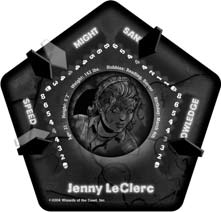
\includegraphics[width=6cm]{resources/traits}
\end{center}

Jede Eigenschaft zeigt auch ein Schädelsymbol. Sinkt eine Eigenschaft auf das Schädelsymbol nachdem der Spuk begonnen hat stirbt dein Charakter. Vor Beginn des Spuks kann niemand sterben. Jede Eigenschaft verbleibt dann immer mindestens auf der Stufe über dem Schädel, auch wenn die Eigenschaft reduziert werden müsste.

Physischer Schaden wird nach belieben zwischen \might\ und \speed\ aufgeteilt. Du bewegst die Clips so viele Stufen nach unten, wie du Schaden erlitten hast.

Mentaler Schaden wird zwischen \sanity\ und \know\ aufgeteilt.

Im Beispielbild hat Jenny 3 physischen Schaden erlitten.

\subsection{Spielablauf}

Angefangen beim Startspieler führt jeder Spieler im Uhrzeigersinn einen Entdeckungszug im Haus durch.

\subsection{Wenn du am Zug bist …}
… kannst du beliebig viele der folgenden Aktionen durchführen, egal in welcher Reihenfolge:

\begin{itemize}
    \item Du kannst dich bewegen.
    \item Du kannst einen neuen Raum entdecken.
    \item Du kannst Item- oder Omenkarten einsetzen.
    \item Du kannst würfeln.
    \item Du kannst angreifen (einmal pro Zug nachdem der Spuk begonnen hat).
\end{itemize}

Solange der Spuk noch nicht begonnen hat, musst du am Ende deines Zuges einen Spuk-Wurf machen (siehe Spuk-Wurf durchführen auf Seite \pageref{kap:rule:makehauntroll}), wenn du zuvor in dieser Runde eine Omenkarte gezogen hast. Das Spiel bekommt einige neue Wendungen sobald der Spuk beginnt (siehe in
„Der Spuk“ auf Seite \pageref{kap:rule:haunt}).


\subsubsection{Bewegen}

Wenn du am Zug bist kannst du so viele Felder weit laufen, wie es deine SPEED-Anzeige auf deiner Charakterkarte anzeigt. Du kannst Aktionen wie Angriffe oder das Benutzen eines Gegenstandes unterwegs ausführen. Wenn es sich im Spiel ergibt, dass du eine Karte ziehen musst, ist deine Bewegung für diese Runde beendet. Anderfalls darfst du weitere Räume entdecken.

\paragraph{Beispiel für eine Bewegung:} … (Stimmt nicht ganz im englischen Orginal :)

\subsubsection{Entdecken eines neuen Raumes}
\label{kap:rule:discoverroom}

Wenn deine Figur eine Tür betritt und sich auf der anderen Seite kein Raum befindet, nimm dir das oberste Feld vom Raum-Stapel. Wenn es die gleiche Etage anzeigt wie die auf der du dich gerade befindest, legst du das Feld einfach an dieser Tür an und betrittst das Feld mit deiner Figur. Lege jedes neue Raumfeld so logisch wie möglich an, so dass immer angrenzende Räume entstehen die durch die Türen verbunden werden. (Verbinde Türöffnungen immer wenn es möglich ist. Türen, die auf Wände zeigen werden zu Scheintüren.)

Falls das gezogene Raum-Feld nicht zu deiner momentanen Etage passt, lege es verdeckt auf einen Ablagestapel. Ziehe auf diese Weise so lange neue Felder nach bis ein passendes gefunden ist. (Einige Felder können auf mehreren Etagen eingesetzt werden.)

Abenteurer können nicht durch Scheintüren gehen. Scheinfenster (falsche Fenster, also Fenster mit dahinterliegender fester Wand) zählen nicht als Fenster im Sinne von offenen Fenstern bei Events oder in einer Spukbeschreibung, es sei denn es steht explizit das Gegenteil geschrieben.

Ein Abenteurer kann jederzeit durch eine Tür gehen wenn sie mit einem angrenzenden Raum verbunden ist. Türen sind immer offen. Die einzige Ausnahme bildet die Eingangstür in der ENTRANCE HALL. Sie ist immer verschlossen. Du kannst das Haus nicht verlassen es sei denn ein Spuk-Szenario erlaubt es dir. (Freiluft-Räume gehören ebenfalls zum Haus.)

Treppen verbinden Etagen miteinander. Die große Treppe im Eingangsbereich führt immer zum Obergeschoß. Die Treppen im Keller führen immer zum und vom Foyer durch eine geheime Tür. (Du kannst die Kellertreppen erst benutzen wenn du sie im Keller entdeckt
hast.)

Einige Räume haben bestimmte Auswirkungen auf deinen Charakter, wenn er diesen Raum betritt. Auf manche Raumkarten sind spezielle Regeln aufgedruckt, die beim Eintreten oder Verlassen aktiviert werden. Gehören zu einem Raum sowohl ein Regeltext als auch ein Symbol, wird die entsprechende Karte zuerst gezogen und ausgeführt.

Manche Räume beeinflussen auch die Bewegung. Einige besondere Räume sind auch noch mal in dem Abschnitt „Spezielle Räume“ auf Seite \pageref{kap:rules:specialrooms} erklärt.


\subsubsection{Kann ich ein Stockwerk durch das Legen eines neuen Raumes abschließen?}

Nein, du darfst Räume nicht so anlegen, dass alle Türen in dem Stockwerk miteinander verbunden sind. Wenn es keine bessere Anlegestelle für einen Raum gibt, ziehe eine andere Raumkarte, solange, bis du eine findest, die eine Tür frei lässt. Gibt es keine Raumkarte mehr, mit der dies möglich ist, ordne die bestehenden Räume so um, dass es wieder offene Türen gibt.

\subsubsection{Was passiert, wenn der Raumstapel leer ist?}

Mische die Karten, die du beim Benutzen des Raumstapels beiseitegelegt hast und fange erneut mit diesen an.

Gibt es überhaupt keine Räume für ein Stockwerk mehr, hast du das Stockwerk / Haus vollständig entdeckt.

\subsubsection{Ziehen von Omen-, Gegenstand- oder Ereigniskarten}

Ein gezogenes Raum-Feld kann ein Kartensymbol enthalten. Wenn du das erste Mal einen Raum mit einem Kartensymbol ziehst, endet dein Zug in diesem Raum und du ziehst die entsprechende Karte. Nur der erste Spieler, der einen Raum betritt, zieht eine Karte.

Wenn der Raum ein Spiral-Symbol hat, ziehst du eine EVENT-Karte. Lese sie laut vor und folge den Anweisungen die auch beinhalten können, dass du würfeln musst. Danach wird die Karte abgelegt falls dort nichts Gegensätzliches angegeben ist oder die Karte noch weiterführende Auswirkungen hat.

Wenn der Raum ein Stierkopf-Symbol hat, ziehst Du eine ITEM-Karte. Sie wird laut vorgelesen und offen vor dir abgelegt; somit hast du diesen Gegenstand in deinem Besitz. Du kannst ihn sofort und pro Zug einmal benutzen wenn nichts anderes auf der Karte
angegeben ist.

Wenn der Raum ein Raben-Symbol hat, ziehst du eine OMEN-Karte. Lies sie laut vor und lege sie dann offen vor dir ab. Es kann sein das du nun sofort etwas tun musst. Am Ende deines Zuges musst Du auf jeden Fall einen „Spuk-Wurf“ durchführen, wenn der Spuk noch nicht begonnen hat (Seite \pageref{kap:rule:makehauntroll}).

Wenn du aufgrund eines Effektes einen neuen Raum ziehen musst, und dieser neue Raum ein Symbol hat, ziehst du die entsprechende Karte. Wird ein Raum aus anderen Gründen angefügt, z.B. wegen Anweisungen im Spukbuch, zieht der erste Spieler, der diesen Raum betritt, keine Karte.

Auch wenn deine Bewegung mit dem Ziehen einer Karte endet, kannst du immer noch Gegenstände benutzen, angreifen, …

\subsubsection{Spezielle Räume}
\label{kap:rules:specialrooms}

Viele Räume haben Besonderheiten die auf dem Feld angegeben sind. Einige von ihnen haben aber auch noch spezielle Eigenschaften die hier aufgelistet werden:

\paragraph{CHASM, CATACOMBS, THE VAULT und TOWER}

Dies sind alles Sperr-Räume. Eine Sperre kann verhindern, dass du den dahinter liegenden Raum betrittst. Um ihn zu durchqueren muss man einen auf dem Feld angegebenen Wurf durchführen. Diesen Wurf kannst du einmal pro Runde versuchen. Das Durchqueren der Sperre kostet keinen Bewegungspunkt. Wenn der Wurf misslingt, musst du stehen bleiben. In deinem nächsten Zug kannst du es erneut versuchen oder du gehst den Weg zurück auf dem du gekommen bist.

Abenteurer können nicht mit anderen Abenteurern, die sich auf der anderen Seite einer Sperre aufhalten, interagieren oder sie angreifen. Monster ignorieren Sperren, aber wenn ein Monster seine Bewegung in einem Sperr-Raum beendet muss der Verräter entscheiden, auf welcher Seite der Sperre das Monster anhält.

Wenn ein Effekt dich in einem Sperr-Raum absetzt, kannst du entscheiden, auf welcher Seite du landest. Wenn ein Marker in dem Raum abgelegt werden muss (z.B. Geheimgang), bleibt dieser Marker dauerhaft auf der gewählten Seite.

\paragraph{ENTRANCE HALL (Die Eingangshalle) \& Co.}

Die Eingangshalle, das Foyer und die große Treppe befinden sich alle auf einem Feld gelten aber trotzdem als drei verschiedene Räume. THE GRAND STAIRCASE und UPPER LANDING gelten als zwei verschiedene Räume.


\paragraph{THE COAL CHUTE (Der Kohlenschacht)}

Betrete den Kohlenschacht, um mit einem Schritt zum BASEMENT LANDING zu kommen. Ein Zug eines Entdeckers oder Monsters kann nicht auf dem Kohlenschacht enden. (Die Figur landet automatisch im BASEMENT LANDING .)

\paragraph{THE COLLAPSED ROOM (Der zusammengefallene Raum)}

Nur der Spieler der als erstes diesen Raum entdeckt muss den dort angegebenen „Geschwindigkeits-Wurf“ ausführen. Danach können alle Spieler die diesen Raum betreten dies ignorieren, allerdings können sie es auch ausführen. In diesem Fall muss der Spieler aber auch den evtl. Schaden in Kauf nehmen. Das Herunterfallen in den Keller zählt nicht als Schritt für die Bewegung, der Spieler nimmt trotzdem Schaden.

Nur der erste Spieler, der in das Loch fällt, wählt ein Keller-Feld und legt es an. Auf dieses Feld wir dann der Marker BELOW COLLAPSED ROOM abgelegt und jeder weitere Spieler der herunterfällt landet in diesem Raum. Lege das neue Keller-Feld an die bestehenden Kellerräume an. Gibt es keine Kellerräume mehr, wähle einen bestehenden Raum als Zielraum aus.

Ist der erste Charakter, der den eingestürzten Raum betritt, ein Monster, setze das Monster in einen beliebigen Kellerraum und ziehe keinen neuen Raum.

\paragraph{JUNK ROOM (Rumpelkammer)}

Bremst dich dieser Raum beim Verlassen und deine verbleibende Bewegung würde dich am Verlassen hindern, kommst du dennoch heraus. Du bleibst im Nachbarraum stehen.

\paragraph{THE MYSTIC ELEVATOR (Der mysteriöse Fahrstuhl)}

Dieses Feld bewegt sich, sobald es betreten wird. Würfel mit zwei Würfeln und lege dieses Feld an eine Tür der erwürfelten Etage an. (Wenn sich dort keine befindet bleibt der Fahrstuhl dort wo er ist.) Wenn du die Etage erwürfelst, auf der du dich gerade befindest, kannst du ihn an eine andere Tür dieser Etage legen. Der Fahrstuhl kann nur einmal pro Zug benutzt werden.

Monster und der Verräter können das Fahrstuhlziel ohne zu würfeln beliebig wählen. Der Fahrstuhl kann sich jedoch nur einmal pro Verräterzug inklusive aller Monsterzüge bewegen. In anderen Worten: Verwendet der Verräter den Fahrstuhl für seine Figur, funktioniert er nicht mehr, wenn Monster im folgenden Monsterzug den Fahrstuhl benutzen wollen.

Ein Held muss den Fahrstuhlwurf ausführen, sobald er den Fahrstuhl betritt oder wenn er seinen Zug ohne Bewegung im Fahrstuhl verharrt hat.

Wenn sich mehrere Spieler im Fahrstuhl aufhalten, und ein anderer Spieler tritt ein und würfelt eine 0, nehmen alle Spieler im Fahrstuhl schaden.

Wenn ein Effekt in den Fahrstuhl führt (z.B. der eingestürzte Raum oder der Geheimgang), verbleibt der entsprechende Marker im Fahrstuhl, auch wenn sich dieser bewegt.

\paragraph{THE VAULT (Der Tresorraum)}

Landet ein Spieler durch einen Effekt in diesem Raum, befindet er sich außerhalb der verschlossenen Tür. Sobald das Gewölbe einmal geöffnet wurde, wird der Marker EMPTY VAULT dort abgelegt. Der Verräter öffnet den Tresor nicht automatisch, er muss zum Öffnen auch den Wurf bestehen.

%\paragraph{THE CRYPT (Die Gruft)}
%
%Monster ignorieren die Auswirkungen dieses Raumes.
%
%\paragraph{THE FURNACE ROOM (Der Heizraum)}
%
%Monster ignorieren die Auswirkungen dieses Raumes.

\subsubsection{Benutzen von Gegenstand- und Omenkarten}
\label{kap:rule:useitemomen}

Alle Abenteurer können ihre Gegenstände einmal pro Zug benutzen. Manche Monster können das ebenfalls, wenn die Spukregeln es erlauben. Die meisten Omen-Karten (ausgenommen der Karte BITE) sind ebenfalls Gegenstände, die man nehmen und benutzen kann wie ITEM-Gegenstände. Es gibt keine maximale Anzahl an gleichzeitig tragbaren Gegenständen.

Einmal während deines Zuges kannst du (oder ein Monster) folgendes tun:
  \begin{itemize}
    \item Einen Gegenstand einem anderen Mitspieler geben, der sich im selben Raum wie du befindet (wenn beide einverstanden sind).
    \item Gegenstände fallen lassen. (Wenn du das tust, musst du einen fünfeckigen ITEM-Marker im Raum ablegen.) Ein anderer Spieler oder auch du selbst, kann diesen Gegenstand (oder auch mehrere gleichzeitig) später aufheben.
    \item Hebe einen oder mehrere Gegenstände aus dem Raum auf. Entferne die Marker entsprechend.
\end{itemize}

Einige Gegenstände können nicht getauscht werden. Sie können jedoch abgelegt und aufgehoben werden. Der Text auf der Karte gibt an, ob eine solche Aktion verboten ist.

Der Hund, der Biss, das Mädchen und der Verrückte sind keine richtigen Gegenstände und können daher nicht getauscht, gestohlen oder abgelegt werden.

Mit jedem Gegenstand kann ein Spieler \emph{eine} der folgenden Aktionen pro Runde durchgeführen:

  \begin{itemize}
        \bitem Den Gegenstand benutzen.
        \bitem Den Gegenstand mit anderen Spieler handeln.
        \bitem Den Gegenstand fallen lassen.
        \bitem Den Gegenstand stehlen (Siehe ``\nameref{kap:rule:specialattack}'' auf Seite \pageref{kap:rule:specialattack}).
        \bitem Den Gegenstand aufheben.
  \end{itemize}

Einen Gegenstand zu benutzen bedeutet zu attackieren oder einen Würfelwurf zu versuchen oder jede andere Aktion, in die der Gegenstand verwickelt ist. Ein Spieler kann z.B. den Speer nicht benutzen und ihn im selben Zug einem anderen Spieler geben.

Wenn ein Gegenstand einen deiner Charakterwerte über seinen Maximalwert hebt, notiere dir, wieviele Stufen der Wert über dem Maximum liegt. Verlierst du im weiteren Spielverlauf Stufen, nehme zunächst von den separat notierten Stufen Schaden.

\paragraph{Item-Marker}

Viele Spukszenarien legen ITEM-Marker ins Haus, für deren Benutzung spezielle Regeln gelten. Bestimmen es die Spukregeln nicht anders, können diese ITEM-Marker wie OMEN und ITEMS gehandelt, abgelegt oder gestohlen werden.

\paragraph{Waffen} Die Axt, der Blutdolch, der Revolver, der Speer und der Opferdolch sind Waffen. Waffen können nur während einer Attacke benutzt werden und nicht zur Verteidigung. Du kannst für eine Attacke nur eine Waffe benutzen, aber du kannst mehr als eine tragen. Eine Waffe zu benutzen ist optional.

\paragraph{Gefährten}
Der Hund, der Biss, das Mädchen und der Verrückte sind Gefährten, die dem Charakter folgen, der die Obhut über sie hat. Gefährten haben keine physischen oder mentalen Eigenschaften.

Kartenanweisungen haben immer Vorrang gegenüber den allgemeinen Regeln!

\subsubsection{Was passiert, wenn sich Regeln wiedersprechen?}

Anweisungen auf Karten haben Vorrang vor Regeln aus dem Regelbuch.

\subsubsection{Durchführung eines Wurfes}

Sehr oft während des Spiels muss gewürfelt werden. Zum Beispiel für eine Karte oder wenn man einen Raum betritt.

Es gibt keine Grenze für Würfelwürfe pro Zug, allerdings kannst du den gleichen Wurf nicht mehrfach probieren. Du kannst beispielsweise nicht mehrfach pro Zug versuchen, den Tresor zu öffen.

Wenn dir eine Karte sagt, eine bestimmte Anzahl von Würfeln zu würfeln, tue es und zähle die Punkte auf den einzelnen Würfeln zusammen. Führe dann aus was die Karte für dieses Ergebnis vorgibt.

\paragraph{Schadenswürfe} Lautet ein Effekt ``Nehme \emph{einen Würfel} physischen Schaden'' (``Take \emph{one die} of physical damage'') würfle einen Würfel. Du nimmst Schaden in \might\ und/oder \speed\ entsprechend der gewürfelten \emph{Augenzahl}. Für Effekte die mehrere Würfel Schaden verursachen addiere die Augen auf allen Würfeln. \emph{Mentaler Schaden} (Mental Damage) funktioniert genauso, nur dass du hier den Schaden nach belieben zwischen \sanity\ und \know\ aufteilen musst.

\paragraph{Charakterwürfe (Trait rolls)} Manchmal sagt dir eine Karte oder ein Raum, dass du auf eine deiner Eigenschaften (Bewegung, Kraft, Gesundheit oder Wissen) würfeln sollst. In diesem Fall nimmst du so viele Würfel wie der momentane Wert deiner geforderten Eigenschaft ist und würfelst.

Wenn du zum Beispiel einen Wurf auf Gesundheit durchführen musst und der Wert deiner Gesundheit vier ist, dann kannst du vier Würfel werfen. Zähle die Punkte zusammen und schaue nach was du aufgrund des Ergebnisses tun musst.

\paragraph{Würfe für Aufgaben} Manche Spukszenarien verlangen Würfe für bestimmte Aufgaben wie z.B. einen Exorzismus. Du kannst einen Aufgabenwurf nur einmal pro Zug versuchen. Das gilt auch, wenn es mehrere Würfe gibt, die die Aufgabe erfüllen würden (z.B. lassen sich Exorzismen sowohl mit \sanity-Würfen als auch mit \know-Würfen durchführen.)

\subsubsection{Einen Angriff durchführen}
\label{kap:rule:attack}

\textbf{Du kannst erst angreifen, wenn der Spuk begonnen hat.}

Einmal während deines Zuges darfst du einen Gegner attackieren, der sich im selben Raum wie du befindet.  (Ein Gegner ist ein Abenteurer oder Monster, das dich aufhalten oder stören will).

Bei einem Angriff würfelst du mit so vielen Würfeln wie es deinem Wert in der Eigenschaft \might\ entspricht. Dein Gegner tut das gleiche. Der Spieler mit der höheren Augenzahl gewinnt und fügt dem Kontrahenten physischen Schaden zu. Die Höhe des Schadens ergibt sich aus der Differenz der beiden Ergebnisse. (Beispiel: Wenn du eine 6 würfelst und dein Gegner nur eine 5, dann erhält er 1 Punkt physischen Schaden.) Bei einem Unentschieden
erhält niemand Schaden.

Es kann vorkommen, dass dir eine Karte oder ein Spuk befiehlt, mit einem anderen Wert als \might\ zu attackieren. Dies wird dann genau so durchgeführt wie vorher beschrieben, dein Gegner und du benutzen einfach nur eine andere Eigenschaft. So müssen bei einer \speed -Attacke z.B. beide Spieler auf ihrem Bewegungswert würfeln. \speed -Attacken verursachen ebenfalls physischen Schaden.

Wenn eine Karte oder ein Spuk eine Attacke mit \sanity\ (Gesundheit) oder \know\ (Wissen) verlangt, verursacht dies \emph{mentalen Schaden}. In diesem Fall müssen die Schadenspunkte im Bereich \sanity\ und/oder \know\ verringert werden.

Bei \emph{physischen Schäden} verringert man seine Werte im Bereich \might\ und/oder \speed\ um so viele Punkte wie die Differenz ergeben hat.

Du kannst einen Gegner nicht in einem Bereich attackieren den er nicht besitzt. Wenn z.B. ein Monster keine \sanity-Eigenschaft hat, kannst du ihn in diesem Bereich nicht angreifen.

In einigen Fällen kann es sein, dass du bei einer Attacke einem Gegner keinen Schaden zufügst sondern ihm z.B. etwas stiehlst (siehe ``Spezial-Attacken'' auf Seite \pageref{kap:rule:specialattack}).

Monster sind lediglich betäubt wenn man sie besiegt, außer ein Spukszenario besagt etwas anderes. (siehe ``Wie Monster funktionieren'' auf Seite \pageref{kap:rules:monsters}). Du kannst ein betäubtes Monster angreifen, wenn es andere Effekte auslöst (z.B. stehlen oder es mit einem speziellen Gegenstand töten). Betäubte Monster werfen immer noch Verteidigungswürfe, aber angreifende Helden tragen im Falle einer Niederlage keinen Schaden mehr davon.

Du kannst während eines Zuges sowohl eine spezielle Spukaktion als auch einen normalen Angriff durchführen.

%% ??
Wenn der Spuk einmal begonnen hat und irgendeiner deiner Werte auf das Totenkopf-Symbol gesunken ist stirbst du. Vor dem Spuk kann niemand sterben –- d.h. kein Wert einer Eigenschaft kann tiefer sinken als die niedrigste Stufe vor dem Totenkopf-Symbol.



\subsubsection{Spezial-Attacken}
\label{kap:rule:specialattack}

\paragraph{Distanz-Angriff} Der Revolver erlaubt es dir, jemanden in einem Raum anzugreifen der sich in deiner Sichtweite befindet – ein Pfad der durch eine ununterbrochene Linie durch Türen führt. Du selbst erleidest keinen Schaden wenn dein Gegner dich beim Würfeln besiegt. Einige Monster können aber auch Distanz-Angriffe durchführen.

\paragraph{Gegenstände stehlen} Wenn du jemanden angreifst und 2 oder mehr Punkte physischen Schaden verursachst, kannst du statt Schaden zu verursachen auch einen handelbaren (tradeable) Gegenstand oder Omen stehlen. Fernangriffe ermöglichen kein Stehlen.

Manche Spukszenarien haben spezielle Diebstahlregeln.

\subsubsection{Beispiel für einen Angriff}

Jenny greift einen Werwolf an. Sie hat einen \might-Wert von 4, also würfelt sie mit 4 Würfeln ihren Angriff. Sie würfelt 5 Augen. Der Verräter würfelt 8 Augen für den Werwolf. Jenny nimmt jetzt 8-5=3 Punkte physischen Schaden. Sie entscheidet sich, ihre Kraft um 2 Stufen und ihre Geschwindigkeit um 1 Stufe zu erniedrigen. Jenny lebt noch, aber sie ist verletzt.

\subsection{Der Spuk}
\label{kap:rule:haunt}

Sobald der Spuk beginnt, ändert sich das Spiel dramatisch. Es wandelt sich in einen verzweifelten Wettkampf um den Sieg.

\subsubsection{Durchführen eines Spuk-Wurfes}
\label{kap:rule:makehauntroll}

Bevor der Spuk beginnt, musst du, wenn du in diesem Zug eine Omen-Karte gezogen hast, immer am Ende deines Zuges mit 6 Würfeln würfeln. Dies nennt man einen Spuk-Wurf. Wenn du weniger Augen würfelst als die Anzahl gezogener Omen-Karten von allen Spielern beginnt der Spuk. Derjenige der den Spuk mit seinem Wurf ausgelöst hat wird „Spuk-Verursacher“ genannt.

Beispiel: Du ziehst in deinem Zug eine Omen-Karte und die anderen Spieler haben bisher 4 Omen-Karten gezogen. Um den Spuk zu beginnen müsstest du 4 Augen oder weniger würfeln.

\subsubsection{Auslösen des Spuks}

Der „Spuk-Verursacher“ nimmt sich nun das „Buch des Verräters“ und schaut dort in der Tabelle nach, welcher Spuk ausgelöst worden ist... und vor allem wer der Verräter ist.

Die Tabelle zeigt oben eine Liste der Omen-Karten und an der Seite eine Aufstellung aller Räume. Suche nun nach der Omen-Karte, bei der der Spuk ausgelöst worden ist und den Raum, in dem sich die Figur des „Spuk-Verursachers“ befand, als der Spuk begann. Dort wo die Spalten/Zeilen sich treffen findet man die Nummer für das zu spielende Spuk-Szenario.

Die Liste unterhalb gibt an, wer zum Verräter wird. Nachdem du auf diese Weise herausgefunden hast wer der Verräter ist, gib demjenigen das „Buch des Verräters“. Der „Spuk-Verursacher“ ist also \emph{nicht} zwangsläufig auch der Verräter.

\paragraph{Sonderfall:} Wenn zwei oder mehr Spieler als Verräter in Frage kommen und einer von ihnen der „Spuk-Verursacher“ ist, dann wird diese Person auch zum Verräter. Wenn keiner der in Frage kommenden der „Spuk-Verursacher“ war, wird es derjenige, der als nächstes im Uhrzeigersinn nach dem „Spuk-Verursacher“ sitzt.

\subsubsection{Spuk-Vorbereitungen}

Folgendes muss beim Start des Spuks getan werden:

\begin{itemize}
    \item Der Verräter nimmt sich das „Buch des Verräters“ und verlässt damit den Raum. Er liest dann \emph{nur} das Szenario, das nun beginnt. Dieser Spieler muss auch die Regeln ``Die neuen Fähigkeiten des Verräters'' (Seite \pageref{kap:rule:newtraitorpowers}) und ``Wie Monster funktionieren'' (Seite \pageref{kap:rules:monsters}) kennen. Kennt er sie noch nicht, sollte er sie sich von einem Mitspieler erklären lassen oder das Regelbuch mitnehmen.
    \item Alle anderen Spieler werden zu Helden. Sie schauen sich das gleiche Szenario in dem Buch „Geheimnisse des Überlebens“ an. Die Helden sollten sich auch kurz einen Plan zurechtlegen, um zu überleben.
    \item Wenn beide Parteien fertig sind kehrt der Verräter in den Raum zurück. Nun tun alle das, was im Szenario unter der Rubrik „Right Now“ bzw. ``Was ihr jetzt tun müsst'' stand. (Zum Beispiel das Platzieren von Markern im Haus oder das Ziehen von Karten.)
\end{itemize}

\subsubsection{Zugreihenfolge nach Beginn des Spuks}

Es beginnt immer der Spieler, der links neben dem Verräter sitzt und es geht dann im Uhrzeigersinn weiter. Jeder der Helden hat somit zunächst einen Helden-Zug. Danach macht der Verräter seinen Verräter-Zug. Zum Schluss ist der Verräter noch einmal an der Reihe und zieht die Monster in dem Monster-Zug. (Somit hat ein Spieler zwei Züge: Einen für die Verräter-Figur und einen für die Monster.) Dann ist wieder der Held links vom Verräter dran usw.

\textbf{Die Helden und der Verräter sind weiterhin Abenteurer.} Sie können die gleichen Dinge tun bzw. nicht tun wie vor Beginn des Spuks. Lediglich die Spuk-Würfe, die durch die Omen-Karten ausgelöst wurden, entfallen ab jetzt. Der Verräter muss den Helden in jedem Zug sagen, was er gerade macht, aber nicht warum. Das gleiche gilt anders herum auch für die Helden.

\textbf{Nach Beginn des Spuks können Abenteurer sterben.} Wenn einer der vier Eigenschaftswerte auf das Totenkopf-Level sinkt, dann stirbt dieser Abenteurer. In einigen Spuk-Szenarien kann es sein, dass gestorbene Helden ebenfalls zu Verrätern werden. Manche Spukszenarien erfordern, dass etwas entsprechend der Anzahl der Spieler gemacht wird. Diese Anzahl schließt auch tote Spieler mit ein.

Der Verräter hat immer einen Zug nachdem die Helden an der Reihe waren. Auch wenn der Verräter stirbt kann es sein, dass die Monster allein noch das Ziel des Verräters erreichen können. In diesem Fall führt der Verräter weiterhin den Monster-Zug aus.

Wenn während dem Zug ein Spieler im Haus etwas mittels \know-Wurf herausfindet, wissen die anderen Spieler ebenfalls sofort bescheid.

\subsubsection{An gegnerischen Figuren vorbeiziehen}

Für jeden Gegner der sich nach dem Beginn des Spuks mit dir im selben Raum befindet, muss ein Entdecker einen Extra-Schritt aufbringen um den Raum zu verlassen. (Helden verlangsamen den Verräter und Monster und umgekehrt).

%Ein Gegner ist ein Monster oder Abenteurer der deine Bewegung zu stoppen versucht.
Unabhängig davon, wie viele Bewegungspunkte man hat, kann man immer mindestens ein Feld gehen. Das gilt auch für Monster, die 0 Augen für ihre Bewegung würfeln.

Betäubte Monster verlangsamen die Bewegung eines Abenteurers nicht!

\subsection{Die neuen Fähigkeiten des Verräters}
\label{kap:rule:newtraitorpowers}

Wenn ein Abenteurer zum Verräter wird und von einer zuvor gezogenen Karte negativ beeinflusst wird, z.B. Debris / Schutt, Web / Spinnennetz, entledigt er sich sofort des Effekts. Zusätzlich bekommt er die folgenden neuen Fähigkeiten (außer ein Spuk-Szenario besagt etwas anderes):

  \begin{itemize}
    \item Du kannst alle positiven Raumeffekte benutzen während du negativen ignorierst. Du kannst durch die Drehende Wand (Revolving Wall) schlüpfen ohne zu würfeln. Du kannst entscheiden wo der mystische Fahrstuhl hinfährt.Du landest immer noch im Basement Landing, wenn du die Kohleschütte herunterrutscht.
    \item Du kannst dich von Auswirkungen einer Ereigniskarte oder des BITE-Omens ausschließen lassen. Wenn du eine solche Karte annimmst, musst du auch die negativen Konsequenzen akzeptieren. Du darfst dir die Karte vorher durchlesen.
    \item \textbf{Nach deinem Zug kannst du alle beteiligten Monster bewegen und mit ihnen angreifen.} Auch wenn der Verräter stirbt, kannst du immer noch die Monster steuern. In einigen Szenarien können auch die Monster alleine die Mission erfüllen.
  \end{itemize}

\subsection{Spukszenarien mit verstecktem Verräter}
\label{kap:rule:hiddentraitor}

Bei manchen Spukszenarien ist der Verräter versteckt. Das bedeutet, dass seine Identität vor den Mitspielern geheim gehalten wird. Wenn ein Spuk einen versteckten Verräter benötigt, nehme so viele Monstermarker einer Farbe, wie es Spieler gibt. Stelle sicher, dass der Chip mit der Nummer 1 auch dabei ist. Mischt die Marker und verteilt sie an alle Spieler, so dass die Zahl verdeckt ist. Derjenige, der die Nummer 1 hat, ist der Verräter. Das Spiel beginnt im Uhrzeigersinn mit dem Spieler links vom Spukaufdecker. Der Marker bleibt verdeckt vor den Spielern liegen.

Spukszenarien mit verstecktem Verräter haben keine Anweisungen im Wälzer des Verräters (Traitors Tome). Alle Ziele werden in den Geheimnissen fürs Überleben (Secrets of Survival) beschrieben, das jeder liest.

Es sei denn, das Szenario gibt andere Anweisungen, kann der Verräter sich jederzeit zu erkennen geben, indem er seinen Marker mit der Nummer 1 umdreht. Der Verräter könnte das beispielsweise machen, um den Auswirkungen einer Falle zu entgehen. Hat der Verräter sich zu Erkennen gegeben, gelten für ihn die normalen Verräterregeln, die teilweise negative Effekte verhindern.

Stirbt ein Entdecker, dreht dieser seien Marker um, um seine Identität zu offenbaren. Kein anderer Spieler (bis auf den Verräter) darf seine Identität während des Spiels offenbaren. Er darf behaupten, er wäre nicht der Verräter, aber beweisen kann er es nicht.

Es sei denn, das Szenario gibt andere Anweisungen, dürfen sich die Entdecker jederzeit gegenseitig attackieren, under der richtigen oder verkehrten Annahme, der Attackierte sei der Verräter. Der Verräter profitiert natürlich von Misstrauen zwischen den Entdeckern.

Es sei denn, das Szenario gibt andere Anweisungen, müssen alle Gespräche offen und für jeden hörbar geführt werden. Zwei Entdecker dürfen sich nicht ohne Kenntnis der anderen miteinander Absprechen.

\subsection{Wie Monster funktionieren}
\label{kap:rules:monsters}

Monster haben etwas andere Eigenschaften als die Abenteurer. Alle nun folgenden Fähigkeiten gelten, so lange ein Szenario nichts anderes sagt. Jedes Monster bewegt sich und führt Aktionen durch bevor sich das nächste bewegt.

  \begin{itemize}
    \item \textbf{Monster bewegen sich unterschiedlich.} Zu Beginn des Monster-Zugs werden für jedes Monster so viele Würfel geworfen, wie es seiner Geschwindigkeit entspricht. Das dabei herauskommende Ergebnis gibt an, wie viele Felder das Monster gehen darf. Bei Gruppen mit dem selbem Monstertyp (z.B. Fledermäuse oder Zombies), wird nur einmal für die ganze Gruppe gewürfelt. Das Ergebnis zählt dann für alle Monster dieser Gruppe.
    \item \textbf{Viele Monster können nicht getötet werden.} Nachdem ein Monster einen Schaden erhalten hat, ist es \textbf{betäubt} und muss in der nächsten Runde aussetzen. Der Marker eines betäubten Monsters wird umgedreht. Am Ende des nächsten Zugs des Monsters wird er wieder auf die richtige Seite gedreht. Betäubte Monster können die Bewegung eines Abenteurers nicht verlangsamen. Auch wenn ein Spukszenario sagt, dass Monster nicht betäubt werden, werden sie dennoch durch Effekte betäubt, die explizit betäuben.
    \item Wie Abenteurer können auch \textbf{Monster nur eine Attacke pro Durchgang ausführen}. Monster benutzen oft andere Eigenschaften zum Angreifen als MIGHT. Sie können aber keine der bereits genannten Spezial-Attacken ausführen (falls nicht anders in einem Szenario angegeben).


    \item Wie auch der Verräter können Monster \textbf{negative Raumeffekte ignorieren}. Monster landen im BASEMENT LANDING, wenn sie die Kohleschütte herunterrutschen. Sie können ohne zu würfeln die drehende Wand (REVOLVING WALL) passieren. Monster können die Kohleschütte und das eingestürzte Zimmer auch aufwärts benutzen und sie können von unten auf die Gallerie klettern. Monster profitieren nicht von Räumen, die eine Eigenschaft verbessern.

    \item \textbf{Monster können spezielle Bewegungsoptionen nutzen}, die auf Karten wie der Geheimtreppe oder dem Geheimdurchgang beschrieben werden.

    \item \textbf{Monster können keine neuen Räume entdecken.}
    \item \textbf{Monster können keine Gegenstände tragen},außer ein Szenario bestimmt etwas anderes. Wenn ein Monster, das Gegenstände tragen darf, betäubt wird, lässt es alle Gegenstände fallen. Lege einen Gegenstand-Marker in den Raum. Es kann sie erst wieder aufheben wenn es wieder aktiv wird (im Normalfall 2 Runden später).

    \item Wenn ein Monster im Keller gefangen ist und die Helden nicht erreichen kann, darf der Verräter in seinem Zug den Raumkartenstapel durchsuchen und die Kellertreppe (STAIRS FROM BASEMENT) im Keller anlegen. Der Kartenstapel wird danach gemsicht. Diese Regel gilt nicht, wenn das Spukszenario den Monstern erlaubt, neue Räume zu entdecken.
  \end{itemize}

\subsubsection{Was passiert mit meiner Ausrüstung wenn ich sterbe?}

Wenn du stirbst und Gefährten bei dir hattest (der Hund, das Mädchen oder den Verrückten), wird der entsprechende Marker in den Raum gelegt, in dem du gestorben bist. Die Omenkarte wird beiseite gelegt. Wenn nun ein anderer Abenteurer den Raum betritt, übernimmt dieser die Obhut über den Gefährten und erhält auch die entsprechende Karte. Andere Gegenstände werden ebenfalls in dem Raum abgelegt und durch Gegenstands-Marker ersetzt. Auch hier können nun andere Spieler diese aufheben und erhalten dann die entsprechenden Karten.

\subsection{Gewinnen}

Die Partei (Verräter oder Helden), die zuerst sein Ziel erreicht, gewinnt. Die Gewinnbedingung steht in der Szenariobeschreibung unter ``Ihr gewinnt, wenn …'' und erfordert manchmal anderes als den Tod der Gegner.

Zum Schluss muss mindestens ein Held überlebt haben, damit die Helden gewinnen können. Der Verräter kann dagegen auch gewinnen, wenn er selbst bereits gestorben ist. In diesem Fall können die Monster das Ziel erreichen.

Hat eine Partei gewonnen, wird die entsprechende Siegbedingung ("Wenn ihr gewinnt … / Wenn du gewinnst …") laut vorgelesen.

\subsection{Glossar}

Dieser Abschnitt definiert einige Begriffe, die häufig im Spiel verwendet werden.

A. d. Ü: Einige zu selbsterklärende Begriffe sind nicht übersetzt.

\paragraph{adjacent / angrenzend:} Angrenzende Räume teilen sich eine Kante. Diagonal bedeutet nicht angrenzend.

\paragraph{attack / Attacke / Angriff:} Entdecker und Monster können erst angreifen, wenn der Spuk begonnen hat. Einmal pro Zug kannst du einen Angriffswurf gegen einen Gegner durchführen.

\paragraph{attack roll / Angriffswurf:} Du und dein Gegner rollen so viele Würfel, wie es ihrem \might-Wert entspricht. Derjenige mit der höheren Augenzahl fügt dem Gegner soviele Stufen Schaden zu, wie es der Augenzahldifferenz entspricht. Beim Patt nimmt niemand Schaden. (Siehe ``\nameref{kap:rule:attack}'' auf Seite \pageref{kap:rule:attack})

\paragraph{distance Attack / Fernangriff:} Einige Waffen oder spezielle Gegenstände eines Spuks erlauben dir einen Gegner in einem anderen Raum \textbf{line of sight / in Sichtlinie} anzugreifen. (Siehe ``\nameref{kap:rule:specialattack}'' auf Seite \pageref{kap:rule:specialattack}). Du nimmst keinen Schaden, wenn du deinen Angriff verlierst.

\paragraph{card / Karte:} Es gibt drei verschiedene Kartentypen: Event / Ereignis, Item / Gegenstand und Omen-Karten. Abenteurer ziehen Karten, wenn sie neue Räume entdecken. Wenn du eine Karte ziehst, lese die Anweisungen laut vor und folge den ihnen.

\paragraph{event card / Ereignisskarte:} Spiralsymbol. Nach befolgen der Anweisungen wird die Karte aus dem Spiel genommen, es sei denn die Anweisungen besagen anderes, oder der Effekt dauert an.

\paragraph{item card / Gegenstandskarte:} Stierkopfsymbol. Lege die Karte aufgedeckt vor dich hin. Du besitzt nun den Gegenstand.
(Siehe ``\nameref{kap:rule:useitemomen}'' auf Seite \pageref{kap:rule:useitemomen})

\paragraph{omen card / Omenkarte:} Rabensymbol. Lege die Karte aufgedeckt vor dich hin. Du besitzt nun das Omen. Eventuell musst du sofort eine Aktion ausführen. Hat der Spuk noch nicht begonnen, musst du einen Spukwurf (siehe Seite \pageref{kap:rule:makehauntroll}) durchführen. Die meisten Omen verhalten sich wie Gegenstände.

\paragraph{character / Charakter:} Entdecker / Abenteurer, Monster und Gegner wie Drakula sind Charaktere.

\paragraph{character card:} Die sechs Charakterkarten mit jeweils einem Charakter auf jeder Seite. Zeigt den Namen, ein Bild, die Charakterwerte (\might, ...) und andere Informationen an.

\paragraph{companion / Gefährte / Begleiter:} Der Hund (Dog), das Mädchen (Girl) und der Verrückte (Madman) sind Gefährten und folgen dem dem Abenteurer, der sie in seiner Obhut hat. Gefährten haben keine physischen (körperlichen / physical traits) Eigenschaften und keine mentalen (geistigen / mental traits) Eigenschaften bzw. Werte.

\paragraph{damage / Schaden:} Viele Räume und Karten, als auch verlorene Angriffe verursachen Schaden. Schaden kann physisch (körperlich / physical) oder mental (geistig / mental) sein. Für jeden Punkt Schaden, den du erleidest, schiebe den entsprechenden Anzeigeclip auf deiner Charakterkarte um einen Schritt nach unten. Du kannst mehrere Punkte \textbf{physischen Schaden} frei zwischen Stärke (\might) und Geschwindigkeit (\speed) aufteilen. \textbf{Mentaler Schaden} wird ebenso auf (geistige) Gesundheit (\sanity) und Wissen (\know) aufgeteilt.

\paragraph{discover / Entdecken:} Läuft ein Abenteurer durch einen Tür ohne angrenzenden Raum, zieht er eine neue Karte vom Raumkartenstapel und legt sie an die Tür. Dann bewegt sich der Entdecker in den Raum hinein und entdeckt ihn. (Siehe ``\nameref{kap:rule:discoverroom}'' auf Seite \pageref{kap:rule:discoverroom}).

\paragraph{dice roll / Würfelwurf:} ``Einen \know-Wurf von 4+ bestehen'' bedeutet: Du würfelst mit so vielen Würfeln, wie die Zahl unter dem Clip der \know-Skala auf deiner Charakterkarte anzeigt. Hast du 4 oder mehr Augen gewürfelt, ist der Wurf \textbf{bestanden} und der entsprechende Effekt tritt in Kraft. Hast du weniger Augen gewürfelt, tritt der Effekt nicht in Kraft und/oder ein anderer Effekt tritt in Kraft. Du darfst einen Wurf nur einmal pro Zug ausführen. Für verschiedene Würfe (z.B. Angriff und \knowroll zum Öffnen der Geheimtür) gibt es aber kein Anzahllimit pro Zug.

\paragraph{task roll / Aufgabenwurf:} Manche Spukszenarien verlangen Würfe für bestimmte Aufgaben wie z.B. einen Exorzismus. Du kannst einen Aufgabenwurf nur einmal pro Zug versuchen. Das gilt auch, wenn es mehrere Würfe gibt, die die Aufgabe erfüllen würden (z.B. lassen sich Exorzismen sowohl mit \sanity-Würfen als auch mit \know-Würfen durchführen.)

\paragraph{doors / Türen:} Türen sind immer offen. (Bis auf die Eingangstür (front door).)

\paragraph{explorer / Entdecker / Abenteurer:} Jeder Spieler, der einen Charakter kontrolliert ist ein Entdecker. Nachdem der Spuk begonnen hat, gehört der Verräter weiterhin zu den Entdeckern.

\paragraph{false feature / Scheintür / Scheinfenster:} Wenn es nicht möglich ist, eine Raumkarte so anzulegen, dass alle Türen und Fenster zusammenpassen, werden stattdessen Scheintüren und -fenster erschaffen. Das sind Türen, die nur so tun als wären sie Türen (wie bei Harry Potter :D). Man kann sich nicht durch Scheintüren bewegen. Scheinfenster zählen nicht als Fenster.

\paragraph{figure / Figur:} Zu jeder Charakterkarte gehört entsprechend der Farben eine Plastikfigur, die im Spiel den Entdecker darstellt.

\paragraph{haunt / Spuk:} Der Spuk beginnt mit dem ersten erfolgreichen Spukwurf (haunt roll). Der Spuk wird in den Spukheften bzw in der Übersetzung in den Kapiteln ``\nameref{kap:sos}'' (Seite \pageref{kap:sos}) und ``\nameref{kap:tt}'' (Seite \pageref{kap:tt}) beschrieben. Für jeden Spuk gibt es andere Regeln, neue Monster und andere Gewinnbedingungen. Ab jetzt können Entdecker sterben. Siehe ``\nameref{kap:rule:haunt}'' auf Seite \pageref{kap:rule:haunt}.

\paragraph{hero / Held:} Alle Entdecker, die nicht Verräter sind, werden Helden (heros) genannt.

\paragraph{traitor / Verräter:} Ein Entdecker verrät seine ehmaligen Kameraden. In manchen Spukszenarien bleibt die Identität des Verräters zunächst geheim. (Siehe ``\nameref{kap:rule:hiddentraitor}'' auf Seite \pageref{kap:rule:hiddentraitor})


\paragraph{haunt roll / Spukwurf:} Wird immer dann am Ende eines Zuges durchgeführt, wenn eine Omenkarte gezogen wurde und der Spuk noch nicht begonnen hat. Würfle mit so vielen Würfeln, wie Omenkarten im Spiel sind. \textbf{A.d.Ü: Diese Anweisung wiederspricht der Anweisung im Kapitel ``\nameref{kap:rule:makehauntroll} / Making a Haunt Roll'' auf Seite \pageref{kap:rule:makehauntroll} bzw. 15 im englischen Handbuch. Dort ist von 6 Würfeln die Rede. Ich denke, 6 Würfel zu benutzen ist die bessere Variante.} (bezüglich Betrayal in der 2. Edition).

\paragraph{haunt revealer / Spukaufdecker:} Der Spieler, dessen Spukwurf den Spuk ausgelöst hat, ist der Spukaufdecker. Der Spukaufdecker schaut in der Spuktabelle (haunt chart), welcher Spuk gespielt wird und wer zum Verräter wird.

\paragraph{haunt-specific Aktion / spezielle Spukaktionen:} Ein Spieler kann sowohl eine Spukaktion (z.B. Exorzismuswurf) als auch einen Angriff im selben Zug durchführen.

\paragraph{item / Gegenstand:} Entdecker können Gegenstände tragen und benutzen, stehlen, ablegen, aufnehmen und abgeben. Setzt ein Spukszenario Itemmarker (item token) ein, können diese Gegenstände wie normale Gegenstände oder Omen ebenfalls getauscht, gestohlen, abgelegt oder aufgenommen werden.

\paragraph{weapon / Waffe:} Die Axt (Axe), der Blutdolch (Blood Dagger), der Revolver (Revolver), der Opferdolch (Sacrificial Dagger) und der Speer (Spear) sind Waffen. Du kannst Waffen nur zum Angriff, nicht jedoch zur Verteidigung nutzen. Du kannst nur eine Waffe pro Angriff nutzen, aber du kannst mehrere gleichzeitig tragen. Man ist nicht gezwungen, eine Waffe zu benutzen.

\paragraph{line of sight / Sichtlinie:} Wenn du eine (gekrümmte) Linie durch ein Reihe gerade hintereinander liegender Türen zu einem anderen Spieler ziehen kannst, befindet dich dieser in Sichtlinie. Das bedeutet, man kann sich nicht direkt neben die Tür stellen und sich so aus der Schusslinie bringen.

\paragraph{move / bewegen:} Ein Spieler hat pro Zug so viele Bewegungsschritte, wie die Zahl unter dem Clip auf der \speed-Skala auf der Charakterkarte (= der \speed-Wert) angibt. Jeder Raum erfordert einen Bewegungsschritt. Für jeden Gegner (opponent) im Raum muss ein Entdecker oder Monster einen extra Bewegungsschritt aufwenden, um den Raum zu verlassen.

\paragraph{opponent / Gegner:} Monster und der Verräter sind Gegner der Helden und umgekehrt.

\paragraph{room / Raum:} Jeder Raum erfordert einen Bewegungsschritt. Auf der Rückseite jeder Raumkarte sind manche Stockwerke beleuchtet, und manche nicht. Ein Raum kann nur in den beleuchteten Stockwerken angelegt werden. Ist ein Symbol abgebildet, muss die entsprechende Karte gezogen werden. Texte werden vorgelesen und befolgt. Nur der Abenteurer, der einen Raum entdeckt bzw. anlegt ist von dem Symbol betroffen (bis auf den Tresorraum).

\paragraph{barrier room / Barriere}: Siehe z.B. der Abgrund (Chasm) auf Seite \pageref{kap:rules:specialrooms}.

\paragraph{stack / Kartenstapel / Deck:} …

\paragraph{steal / stehlen:} Statt Schaden zu verursachen, kann der Angreifer stehlen, wenn der Schaden 2 oder mehr beträgt.

\paragraph{stunned / betäubt:} Monster sterben nicht, sondern sind betäubt. Würde ein Monster Schaden erhalten, wird es stattdessen betäubt und setzt seinen nächsten Zug aus. Betäubte Monster verlangsamen Gegner nicht. Betäubte Monster werden umgedreht (S für stunned).

\paragraph{symbol / Symbol:} …

\paragraph{token / Marker / Chip / Token:} Die kleinen bedruckten Pappchips, die Monster oder Gegenstände repräsentieren.

\paragraph{monster tokens / Monstermarker} gibt es in verschiedenen Farben. Spezielle Monster haben große, runde Marker.
\paragraph{item tokens} sind fünfeckig und durchnummeriert.
\paragraph{tait roll tokens,} z.B. \knowroll-Token / Wissenswurfmarker / Wissenswurfchip / Wissenschip sind dreieckig.
\paragraph{event/room tokens} quadratisch

\paragraph{trait / Charaktereigenschaft, -wert:} Jeder Entdecker hat vier Eigenschaften auf seiner Charakterkarte: Stärke / Macht (\might), Geschwindigkeit (\speed), Wissen (\know) und Gesundheit / geistige Gesundheit (\sanity). Jede Eigenschaft hat einen grün markierten Startwert und einen Maximalwert.

\paragraph{mental traits / mentale Eigenschaften:} \sanity\ und \know.
\paragraph{physische traits / physische oder körperliche Eigenschaften:} \speed\ und \might.

\paragraph{turn / Zug:} … . Wenn der Spuk beginnt, fängt der Spieler an, der links neben dem Verräter sitzt. (Weiter im Uhrzeigersinn.) Nachdem alle Spieler gezogen haben zieht erst der Verräter, dann die Monster, die vom Verräter kontrolliert werden.

\paragraph{use / benutzen:} … . Gegenstände können einmal pro Zug zu einem beliebigen Zeitpunkt innerhalb des Zugs benutzt werden.

\paragraph{window / Fenster:} Einige Zimmer besitzen Fenster auf einer oder mehreren Seiten. Du kannst nicht durch Fenster gehen. Manche Spukszenarien haben spezielle Regeln für Fenster. Das Schlafzimmer (Bedroom), die große Treppe (Grand Staircase), das Herrenschlafzimmer (Master Bedroom), die Kapelle (Chapel) und das Esszimmer (Dining Room) haben Fenster.

\subsection{Was ist, wenn es keine Regel für eine Situation gibt?}

Lasst euch nicht aufhalten. Einige dich mit deinen Mitspielern auf eine sinnvolle Regel. (Bei Uneinigkeit werfe eine Münze.) Spiele weiter.

\end{flushleft}
\setlength\parskip{0pt}

\pagebreak

%\twocolumn
\section{Rooms / Räume}


\begin{itemize}
    \parskip-4pt
    \iroom{Abandoned Room}{Stillgelegter Raum}
    \iroom{Attic}{Dachboden}
    \iroom{Balcony}{Balkon}
    \iroom{Ballroom}{Ballzimmer.}
    \iroom{Basement Landing}{Landeplatz im Keller (Kohleschütte)}
    \iroom{Bedroom}{Schlafzimmer}
    \iroom{Bloody Room}{Blutiges Zimmer}
    \iroom{Catacombs}{Katakomben}
    \iroom{Chapel}{Kapelle}
    \iroom{Charred Room}{verbrannter Raum}
    \iroom{Chasm}{Kluft}
    \iroom{Coal Chute}{Kohleschacht}
    \iroom{Collapsed Room}{Eingestürztes Zimmer}
    \iroom{Conservatory}{Wintergarten}
    \iroom{Creaky Hallway}{Knarrender Hausflur}
    \iroom{Crypt}{Crypta}
    \iroom{Dining Room}{Speisesaal}
    \iroom{Dusty Hallway}{Verstaubter Hausflur}
    \iroom{Furnace Room}{Ofenraum}
    \iroom{Gallery}{Gallerie}
    \iroom{Game Room}{Spielzimmer}
    \iroom{Gardens}{Gärten}
    \iroom{Graveyard}{Friedhof}
    \iroom{Gymnasium}{Turnraum}
    \iroom{Junk Room}{Gerümpelzimmer}
    \iroom{Kitchen}{Küche}
    \iroom{Larder}{Lagerraum}
    \iroom{Library}{Bibliothek}
    \iroom{Master Bedroom}{Herrenschlafzimmer}
    \iroom{Mystic Elevator}{Mystischer Aufzug}
    \iroom{Operating Laboratory}{Operationssaal}
    \iroom{Organ Room}{Orgelzimmer}
    \iroom{Patio}{Patio, Innenhof}
    \iroom{Pentagram Camber}{Pentagramkammer}
    \iroom{Research Laboratory}{Forschungslabor.}
    \iroom{Servants' Quarters}{Quatier des Dieners}
    \iroom{Stairs From Basement}{Kellertreppe}
    \iroom{Statuary Corridor}{Bildhauerkorridor}
    \iroom{Storeroom}{Abstellraum}
    \iroom{Tower}{Turm}
    \iroom{Underground Lake}{Untergrundsee}
    \iroom{Upper Landing}{Oberer Treppenabsatz}
    \iroom{Vault}{Tresorraum}
    \iroom{Wine Cellar}{Weinkeller}
\end{itemize}





\twocolumn

\section{Events / Ereignisse}


\event{A Moment Of Hope}{Ein Moment der Hoffnung}{
    Irgendetwas in diesem Raum fühlt sich seltsam richtig an. Etwas widersteht dem Bösen des Hauses.
}{
    Plaziere einen \emph{Blessing}-Chip (Segnung) in diesem Zimmer.

    Jeder Held verwendet bei jedem Charakterwurf (Might, ...) in diesem Zimmer einen zusätzlichen Würfel.
}

\event{Angry Being}{Böses Wesen}{
    Es schält sich aus dem Schleim an der Wand neben dir hervor.
}{
    Du musst einen \speedroll\ versuchen:
    \rolls
    \roll{5+}{Du kommst davon. \gainspeed{1}.}
    \roll{2-4}{\takediementaldamage{1}}
    \roll{0-1}{\takediephysicalmentaldamage{1}{1}}
    \erolls
}

\event{Bloody Vision}{Blutige Vision}{
    Die Wände in diesem Raum sind getränkt in  Blut. Es tropft von der Decke, fließt die Wände herunter, über Schränke und Möbel und auf deine Schuhe. Im nächsten Augenblick ist es fort.
}{
    Du musst einen \sanityroll\ versuchen:
    \rolls
    \roll{4+}{Du festigst deinen Geist. \gainsanity{1}.}
    \roll{2-3}{\loosesanity{1}.}
    \roll{0-1}{Wenn sich ein Entdecker oder Monster in deinem oder einem angrenzenden Zimmer befinden, musst du ihn/sie/es angreifen (wenn du kannst). Wähle denjenigen mit der niedrigsten \might.}
    \erolls
}


\event{Burning Man}{Brennender Mann}{
    Ein brennender Mann rennt durch den Raum. Seine Haut schlägt Blasen und zerfällt. Ein glutroter Schädel verbleibt, schlägt auf dem Boden auf, rollt und verschwindet.
}{
    Du musst einen \sanityroll\ versuchen:
    \rolls
    \roll{4+}{Es wird heiß am Kragen, du bist aber ansonsten okay. \gainsanity{1}.}
    \roll{2-3}{Raus, raus, du musst hier raus! Setze deinen Entdecker in die Eingangshalle.}
    \roll{0-1}{Du gehst in Flammen auf. \takediephysicaldamage{1} Dann nehme 1 Würfel mentalen Schaden als du die Flammen ausklopfst.}
    \erolls
}

\event{Closet Door}{Schranktür}{
    Die Schranktür dort ist offen... nur einen Spalt. Darin muss sich etwas befinden.
}{
    Lege den \chip{Closet}{Schrank} in dieses Zimmer.

    Einmal während seines Zuges, kann ein Entdecker zwei Würfel werfen, um den Schrank zu öffnen.

    \rolls
    \roll{4}{Ziehe eine \itemcardd .}
    \roll{2-3}{Ziehe eine \eventcard .}
    \roll{0-1}{Ziehe eine \eventcard\ und entferne den \chipe{Closet}.}
    \erolls

}

\event{Creepy Crawlies}{Gruselige Krabbler}{
    Eintausend Käfer stürzen sich aus deiner Haut, kommen unter deiner Kleidung und aus deinen Haaren hervor.
}{
    Du musst einen \sanityroll\ versuchen:
    \rolls
    \roll{5+}{Du blinzelst und sie sind weg. \gainsanity{1}.}
    \roll{1-4}{\loosesanity{1}.}
    \roll{0}{\loosesanity{2}.}
    \erolls

}


\event{Creepy Puppet}{Gruselige Puppe}{
    Du siehst eine dieser Puppen, bei denen dir die Haare zu Berge stehen. Sie springt dich mit einem kleinen Speer in den Händen an.
}{
    Der Spieler zu deiner Rechten wirft einen \mightroll\ mit 4 Würfeln für die Puppe. Du verteidigst dich normal, indem du einen \mightroll\ ausführst.

    Wenn du Schaden davonträgst, erhält der Entdecker mit dem Speer (Spear) 2 \might\ (es sei denn, du besitzt den Speer).
}


\event{Debris}{Schutt}{
    Mörtel fällt von den Wänden und der Decke.
}{
    Du musst einen \speedroll\ versuchen:
    \rolls
    \roll{3+}{Du weichst aus. \gainspeed{1}.}
    \roll{1-2}{Du bist unter Schutt vergraben. \takediephysicaldamage{1}}
    \roll{0}{Du bist unter Schutt vergraben. \takediephysicaldamage{2}}
    \erolls

    Wenn du unter Schutt begraben bist, behalte diese Karte. Du kannst nichts machen, bis du befreit wurdest. Einmal pro Zug kann ein Entdecker einen \mightroll\ versuchen, um dich zu befreien. (Du kannst diesen Wurf ebenfalls versuchen.) 4+ befreit. Nach drei erfolglosen Versuchen befreist du dich in deinem folgenden Zug automatisch und kannst normal agieren.
}

\event{Disquieting Sounds}{Beunruhigende Geräusche}{
    Das Geschrei eines Babys, einsam und verlassen.

    Ein Entsetzensschrei.

    Das Krirschen zerbrechenden Glases.

    Dann: Stille.
}{
    Würfle mit 6 Würfeln. Wenn du genauso viele oder mehr Augen würfelst, als Omen aufgedeckt wurden, erhälst du 1 \sanity.
    Falls nicht, nehme 1 \emph{Würfel} geistigen Schaden.
}

\event{Drip ... Drip ... Drip ...}{Tropf ... Tropf ... Tropf ...}{
    Ein rhythmisches Geräusch nagt an deinem Verstand.
}{
    Lege einen \chip{Drip}{Tröpfeln} in diesen Raum.

    Jeder Entdecker rollt bei jedem Charakterwurf (Might, ...) in diesem Raum mit einem Würfel weniger.
}

\event{Footsteps}{Fußabdrücke}{
    Die Dielen knarren leise. Staub steigt auf. Fußabdrücke erscheinen auf dem schmutzigen Boden. Als sie dich schließlich erreichen, sind sie plötzlich fort.
}{
    Würfle mit einem Würfel. (Befindest du dich in der Kapelle, würfle mit 2 Würfeln.)

    \rolls
    \roll{4}{Du und der nächstgelegene Entdecker erhalten 1 \might.}
    \roll{3}{Du erhälst 1 \might\ und der nächst\-ge\-le\-ge\-ne Entdecker verliert 1 \sanity.}
    \roll{2}{\loosesanity{1}.}
    \roll{1}{\loosespeed{1}.}
    \roll{0}{Jeder Entdecker verliert eine Stufe einer Charaktereigenschaft (Might, ...) seiner Wahl.}
    \erolls
}

\event{Funeral}{Beerdigung}{
    Du siehst einen offenen Sarg. Von innen.
}{
    Du musst einen \sanityroll versuchen:
    \rolls
    \roll{4+}{Du blinzelst und er ist verschwunden. \gainsanity{1}.}
    \roll{2-3}{Die Vision verstört dich. \loosesanity{1}.}
    \roll{0-1}{Du befindest dich wirklich in dem Sarg. Du nimmst 1 \sanity\ und 1 \might\ Schaden, als du dich herausgräbst. Wenn der Friedhof (Graveyard) oder die Crypta (Crypt) entdeckt wurden, versetze deine Figur in einen dieser Räume. (Du wählst aus.)}
    \erolls
}

\event{Grave Dirt}{Grabesschmutz}{
    Dieser Raum ist unter einer dicken Schicht Dreck begraben. Du hustest, als sich der Staub auf deiner Haut und in deinen Lungen absetzt.
}{
    Versuche einen \mightroll:
    \rolls
    \roll{4+}{Du schüttelst den Staub ab. \gainmight{1}.}
    \roll{0-3}{Irgendwas stimmt nicht. Behalte diese Karte. Nehme 1 phsyischen Schaden am Anfang jeder deiner Züge. Lege diese Karte aus dem Spiel, sobald einer deiner Charakterwerte steigt oder du deinen Zug auf dem Balkon, im Garten, auf dem Friedhof, im Turnraum, im Lagerrraum, auf der Veranda oder auf dem Turm beendest. (Balcony, Gardens, Graveyard, Gymnasium, Larder, Patio or Tower)}
    \erolls
}

\event{Groundkeeper}{Hausmeister}{
    Du drehst dich um und siehst einen Mann in Gärtnerkleidung. Er hebt seine Schaufel und greift an. Zentimeter vor deinem Gesicht verschwindet er, einzig matschige Fußabdrücke hinterlassend.
}{
    Versuche einen \knowroll. (Ein Entdecker im Garten verzichtet auf zwei seiner Würfel).

    \rolls
    \roll{4+}{Du findest etwas im Schlamm. Ziehe eine \itemcardd.}
    \roll{0-3}{Der Hausmeister erscheint wieder und schlägt dir die Schaufel ins Gesicht. Der Spieler zu deiner Rechten wirft einen \mightroll\ mit 4 Würfeln für den Hausmeister. Du verteidigst dich normal, indem du einen \mightroll\ ausführst. }
    \erolls
}


\event{Hanged Men}{Die Erhängten}{
    Ein Hauch kühler Luft fährt durch den Raum. Vor dir hängen drei Männer an ausgefransten Seilen. Sie starren dich mit kalten, toten Augen an. Das Trio pendelt sanft im Wind und verschwindet hinter dem Vorhang aus Staub, der von der Decke herabrieselt. Du fängst an zu husten.
}{
    Du musst einen Wurf für jede Charaktereigenschaft (Might, ...) werfen:
    \rolls
    \roll{2+}{Der entsprechende Wert bleibt unbeeinflusst.}
    \roll{0-1}{Du verlierst 1 Stufe der entsprechenden Eigenschaft.}
    \erolls

    Wenn du bei allen 4 Würfen 2+ wirfst, erhälst du einen zusätzlichen Punkt zu einem Charakterwert deiner Wahl.
}


\event{Hideous Shriek}{Scheußliches Kreischen}{
    Es beginnt mit einem Flüstern, aber endet in einem seelenzerreißenden Schrei.
}{
    Jeder Entdecker muss einen \sanityroll\ versuchen:

    \rolls
    \roll{4+}{Du widerstehst dem Geräusch.}
    \roll{1-3}{\takediementaldamage{1}}
    \roll{0}{\takediementaldamage{2}}
    \erolls

    Jedes Ergebnis betrifft nur den Entdecker, der würfelt.
}

\event{Image In The Mirror}{Bild im Spiegel}{
    (Version ohne fettgedruckten Einleitungstext.)
}{
    Es befindet sich ein alter Spiegel im Zimmer. Deine erschrockene Reflektion bewegt sich von alleine. Du erkennst dich, aber in einer anderen Zeit. Deine Reflektion schreibt auf den Spiegel:
    \vspace{\parsep}
    \begin{tightcenter}\begin{bf}DAS WIRD HELFEN\end{bf}\end{tightcenter}
    Dann reicht sie dir einen Gegenstand durch den Spiegel.

    Ziehe eine \itemcardd.
}

\event{Image In The Mirror}{Bild im Spiegel}{
    Wenn du keine \itemcards\ besitzt, gilt dieser Effekt für den nächsten Entdecker zu deiner Linken, der eine \itemcardd\ besitzt. Lege diese Karte aus dem Spiel, wenn niemand eine \itemcardd\ besitzt.
}{
    Es befindet sich ein alter Spiegel im Zimmer. Deine erschrockene Reflektion bewegt sich von alleine. Du erkennst dich, aber in einer anderen Zeit. Du musst deiner Reflektion helfen, also schreibst du auf den Spiegel:
    \vspace{\parsep}
    \begin{tightcenter}\begin{bf}DAS WIRD HELFEN\end{bf}\end{tightcenter}
    Dann reiche einen Gegenstand durch den Spiegel.

    Wähle eine deiner Gegenstandskarten (aber keine \omencard) und lege sie auf das Itemdeck. Dann mische das Deck. Erhalte 1 \know.
}

\event{It Is Meant to be}{So soll es sein}{
    Du brichst auf dem Boden zusammen, Visionen zukünftiger Ereignisse fließen durch deine Gedanken.
}{
    Wähle eine dieser beiden Optionen:
    \rolls
    \roll{$\bullet$}{Schaue dir die drei obersten Karten einer der vier Decks an, vertausche sie nach Wahl und lege sie zurück auf den Kartenstapel. Verrate niemandem dein Wissen.}
    \roll{$\bullet$}{Du kannst stattdessen auch mit vier Wür\-feln werfen und das Ergebnis aufschreiben. Bei irgendeinem zukünftigen Wurf kannst du dieses Ergebnis verwenden anstatt zu wür\-feln. Wenn diese Zahl größer als das maximal mögliche Ergebnis ist, verwende das höchst\-mög\-liche Ergebnis.}
    \erolls
}


\event{Jonah's Turn}{Jonah's Zug}{
    Zwei Jungen spielen mit einem hölzernen Kreisel. ``Willst du auch mal drehen, Jonah?'' fragt einer.

    ``Nein'', sagt Jonah, ``Ich will ihn ganz.'' Jonah nimmt den Kreisel und schlägt dem anderen Jungen ins Gesicht. Der Junge fällt. Jonah schlägt  ihn noch, als der Anblick schwindet.
}{
    Wenn ein Entdecker die Rätsel-Schachtel (Puzzle Box) hat, legt dieser sie aus dem Spiel und zieht stattdessen eine Ersatz-\itemcardd. Wenn dies passiert, erhälst du 1 \sanity. Andernfalls nehme du einen Würfel mentalen Schaden.
}

\event{Lights Out}{Lichter aus}{
    Deine Taschenlampe erlischt. Keine Sorge, jemand anderes hat Batterien.
}{
    Behalte diese Karte. Du kannst pro Zug nur ein Feld laufen bis du deinen Zug bei einem der anderern Entdecker beendest. Lege diese Karte danach aus dem Spiel. Du kannst du nun wieder normal laufen.

    Wenn du die Kerze besitzt oder deinen Zug im Ofenraum (Furnace Room) beendest, lege sie ebenfalls beiseite.
}

\event{Locked Safe}{Verschlossener Safe}{
    Hinter einem Portrait befindet sich ein Wandsafe. Natürlich verklemmt.
}{
    Lege einen \chipe{Safe} in den Raum.

    Einmal pro Runde kann ein Entdecker den Safe mithilfe eines \knowroll\ öffnen:

    \rolls
    \roll{5+}{Ziehe zwei \itemcards\ und entferne den \chipe{Safe}.}
    \roll{2-4}{\takediephysicaldamage{1} Der Safe bleibt verschlossen.}
    \roll{0-1}{\takediephysicaldamage{2} Der Safe bleibt verschlossen.}
    \erolls
}

\event{Mists From The Walls}{Nebel aus den Wänden}{
    Nebel fließt aus den Wänden heraus. Man erkennt Gesichter in dem Dunst, menschliche und ... unmenschliche.
}{
    Jeder Entdecker im Keller (Basement) muss einen \sanityroll\ versuchen:

    \rolls
    \roll{4+}{Die Gesichter sind nur Einbildungen in Licht und Schatten. Alles ist gut.}
    \roll{1-3}{\takediementaldamage{1} (Nehme einen Würfel zusätzlichen mentalen Schaden, wenn sich dein Entdecker in einem Raum mit einem Ereignissymbol befindet.)}
    \roll{0}{\takediementaldamage{1} (Nehme zwei Würfel zusätzlichen mentalen Schaden, wenn sich dein Entdecker in einem Raum mit einem Ereignissymbol befindet.)}
    \erolls

    Jedes Ergebnis betrifft nur den Entdecker, der würfelt.
}

\event{Mystic Slide}{Mystische Rutsche}{
    Bist du im Keller (Basement), betrifft dieses Event den nächsten Entdecker zu deiner Linken, der sich nicht im Keller aufhält. Lege diese Karte aus dem Spiel, wenn alle Entdecker im Keller sind.

    Der Boden vor dir fällt in die Tiefe ab.
}{
    Setze den \chip{Slide}{Rutsche} in diesen Raum, dann versuche einen \mightroll\ um zu rutschen.

    \rolls
    \roll{5+}{Du kontrollierst die Rutsche. Versetze deine Figur in einen Raum deiner Wahl in irgendeinem Stock unterhalb des Ausgangsstockwerks.}
    \roll{0-4}{Ziehe Zimmerkarten bis du eine Kellerkarte ziehst. Plaziere die Karte. (Wenn keine Kellerräume mehr auf dem Stapel liegen, nehme einen bereits existierenden Kellerraum.) Du fällst in diesen Raum und nimmst einen Würfel physischen Schaden. Wenn du nicht an der Reihe bist, ziehe keine Karte für diesen Raum.}
    \erolls

    Ab jetzt kann jeder Entdecker versuchen, zu rutschen.
}


\event{Night View}{Nächtliche Aussicht}{
    Du siehst die Vision eines geisterhaften Pärchens über das Gelände laufen, leise wandelnd in ihrer Hochzeitsgaderobe.
}{
    Du musst einen \knowroll\ versuchen:
    \rolls
    \roll{5+}{Du erkennst die Geister als frühere Bewohner des Hauses. Du rufst ihre Namen, sie drehen sich zu dir um, dunkle Geheimnisse des Hauses flüsternd. \gainknow{1}.}
    \roll{0-4}{Du fährst erschrocken zurück, unfähig zuzusehen.}
    \erolls
}

\event{Phone Call}{Anruf}{
    Ein Telefon klingelt im Zimmer. Du fühlst dich verpflichtet abzunehmen.
}{
    Würfle mit zwei Würfeln. Die zuckersüße Stimme einer alten Frau sagt:
    \rolls
    \roll{4}{``Tee und Kuchen! Tee und Kuchen! Du warst immer mein Liebster.'' \gainsanity{1}.}
    \roll{3}{``Ich bin immer für dich da, mein Süßer. Ich beobachte dich ...'' \gainknow{1}.}
    \roll{1-2}{``Wir sind hier, mein Spatz. Gib uns einen Kuss!'' \takediementaldamage{1}}
    \roll{0}{``Böse kleine Kinder müssen bestraft werden!'' \takediephysicaldamage{2}}
    \erolls
}

\event{Possession}{Besessenheit}{
    Ein Schatten schält sich aus der Wand. Du verharrst starr, als der Schatten dich umrundet und dich bis ins Mark auskühlt.
}{
    Du musst eine Charaktereigenschaft auswählen und für diese einen Wurf versuchen:
    \rolls
    \roll{4+}{Du widerstehst den Verlockungen des Schattens. Erhalte 1 in einem Charakterwert deiner Wahl.}
    \roll{0-3}{Der Schatten zerrt von deiner Energie. Die ausgewählte Eigenschaft sinkt auf die Stufe direkt über dem Schädel. Wenn die Eigenschaft schon auf ihrer niedrigsten Stufe steht, erniedrige eine andere Eigenschaft. }
    \erolls
}

\event{Revolving Wall}{Drehende Wand}{
    Ein Teil der Wand schwingt herum.
}{
    Lege den \chip{Wall-Switch}{Wandschalter} an eine Wand ohne Ausgang oder an eine Ecke in diesem Raum. Wenn es keinen Raum auf der anderen Seite des Wandschalters gibt, ziehe Raumkarten, bis du eine für das entsprechende Stockwerk gefunden hast und lege sie an. (Wenn es für das Stockwerk keine Karten  mehr gibt, nehme diese Karte aus dem Spiel.) Tritt in den Raum ein.

    Einmal während des Zuges eines Entdeckers, wenn sich dieser in einem der beiden vom Wandschalter berührten Räume befindet, kann er/sie einen \knowroll\ versuchen, um den Wandschalter umzulegen:

    \rolls
    \roll{3+}{Der Entdecker findet den versteckten Hebel und geht durch den Durchgang. Dies zählt nicht als Bewegung.}
    \roll{0-2}{Der Entdecker kann den versteckten Hebel nicht finden und den Durchgang nicht passieren.}
    \erolls
}


\event{Rotten}{Verrottet}{
    Der Gestank in diesem Zimmer ist schrecklich.

    Es riecht nach Tod, wie Blut.

    Ein Schlachthausgeruch.
}{
    Du musst einen \sanityroll versuchen:
    \rolls
    \roll{5+}{Verwirrende Gerüche, mehr nicht. \gainsanity{1}.}
    \roll{2-4}{\loosemight{1}.}
    \roll{1}{Verliere 1 \might\ und 1 \speed.}
    \roll{0}{Du krümmst dich vor Übelkeit. Verliere 1 von jeder Charaktereigenschaft.}
    \erolls
}

\event{Secret Passage}{Geheimgang}{
    Ein Bereich der Wand fährt zur Seite. Dahinter erstreckt sich ein modriger Tunnel.
}{
    Lege einen \chip{Secret Passage}{Geheimgang} in diesen Raum. Würfle mit 3 Würfeln und lege den zweiten \chipe{Secret Passage} in:

    \rolls
    \roll{6}{Irgendeinen schon existierenden Raum.}
    \roll{4-5}{Einen existierenden Raum im oberen Stockwerk.}
    \roll{2-3}{Einen existierenden Raum im Erdgeschoss.}
    \roll{0-1}{Einen existierenden Kellerraum.}
    \erolls

    Du kannst nun den Geheimgang nutzen, auch wenn du keine Bewegung mehr übrig hast.

    Die Benutzung des Geheimgangs zählt als eine Bewegung. Der Geheimgang selbst zählt aber nicht als Feld.

    Ab jetzt kann jeder Entdecker den Geheimgang nutzen. Ein Entdecker kann seinen Zug nicht im Geheimgang beenden.
}



\event{Secret Stairs}{Geheimtreppe}{
    Ein schreckliches Knarzen hallt umher. Du hast eine geheime Treppe entdeckt.
}{
    Lege einen \chip{Secret Stairs}{Geheimtreppe} in diesen Raum und einen zweiten \chipe{Secret Stairs} in einen anderen existierenden Raum auf einem anderen Stockwerk. Das verwenden der Geheimtreppe zählt als Bewegung. Die Treppe selbst zählt jedoch nicht als Feld.

    Du kannst den Treppen jetzt folgen, auch wenn du keine Bewegung mehr übrig hast. Wenn du ihnen jetzt folgst, ziehe eine \eventcard\ im nächsten Raum.
}

\event{Shrieking Wind}{Kreischender Wind}{
    Ein Wind zieht durchs Haus, ein langsames Crescendo hin zu einem kreischenden Heulen.
}{
    Jeder Spieler im Garten, auf dem Friedhof, in der Patio, auf dem Turm, auf dem Balkon (Garden, Graveyard, Patio, Tower or Balcony) oder einem Raum mit einem nach draußen führenden Fenster muss einen \mightroll\ versuchen:

    \rolls
    \roll{5+}{Du bleibst auf den Füßen.}
    \roll{3-4}{Der Wind wirft dich um. \takediephysicaldamage{1}}
    \roll{1-2}{Der Wind kühlt deine Seele aus. \takediementaldamage{1}}
    \roll{0}{Der Wind wirft dich derb um. \takediephysicaldamage{1}. Lege einen deiner Gegenstände (wenn du welche hast) in die Eingangshalle (Entrance Hall).}
    \erolls

    Jedes Ergebnis betrifft nur den Entdecker, der würfelt.
}


\event{Silence}{Stille}{
    Im Kellergewölbe wird plötzlich alles Still. Auch das Geräusch des eigenen Atems verstummt.
}{
    Jeder Entdecker im Keller (Basement) muss einen \sanityroll\ versuchen:

    \rolls
    \roll{4+}{Du wartest ruhig bis dein Hörsinn zurückkehrt.}
    \roll{1-3}{Du schreist einen tonlosen Schrei. \takediementaldamage{1} }
    \roll{0}{Du rastest aus. \takediementaldamage{2}}
    \erolls

    Jedes Ergebnis betrifft nur den Entdecker, der würfelt.
}

\event{Skeletons}{Gerippe}{
    Mutter und Kind, sich immer noch umarmend.
}{
    Lege einen \chip{Skeleton}{Skelett} in diesen Raum. Nehme einen Würfel mentalen Schaden.

    Einmal während seines Zuges kann ein Entdecker einen \sanityroll versuchen, um die Skelette zu durchsuchen.

    \rolls
    \roll{5+}{Ziehe eine \itemcardd. Entferne den \chipe{Skeleton}.}
    \roll{0-4}{Du stocherst herum, findest jedoch nichts. \takediementaldamage{1}}
    \erolls

    Jedes Ergebnis betrifft nur den Entdecker, der würfelt.
}

\event{Smoke}{Rauch}{
    Rauch wabert um dich herum. Du hustest während du dir Tränen aus den Augen wischt.
}{
    Lege den \chip{Smoke}{Rauch} in den Raum. Der Rauch blockiert die Sichtlinie von angrenzenden Räumen. Ein Entdecker würfelt mit zwei Würfeln weniger (aber mindestens mit einem Würfel) bei allen Charakterwürfen, während er sich in diesem Zimmer aufhält.
}


\event{Something Hidden}{Etwas Verstecktes}{
    Dieser Raum ist sonderbar, aber weshalb? Es liegt dir fast auf der Zunge.
}{
    Wenn du herausfinden willst, was seltsam ist, versuche einen \knowroll:
    \rolls
    \roll{4+}{Eine Sektion der Wand schiebt sich seitwärts, eine Nische preisgebend. Ziehe eine \itemcardd.}
    \roll{0-3}{Du kannst es einfach nicht herausfinden, was dich ein wenig verrückt macht. \loosesanity{1}.}
    \erolls
}

\event{Something Slimy}{Etwas Schleimiges}{
    Was ist das an deiner Ferse?

    Ein Insekt? Eine Tentakel?

    Eine um sich greifende tote Hand?
}{
    Du musst einen \speedroll\ versuchen:

    \rolls
       \roll{4+}{Du kommst frei. \gainspeed{1}.}
       \roll{1-3}{\loosemight{1}.}
       \roll{0}{Verliere 1 \might\ und 1 \speed.}
       \erolls
}

\event{Spider}{Spinne}{
    Eine faustgroße Spinne landet auf deiner Schulter ... und klettert in deine Haare.
}{
    Du musst einen \speedroll\ versuchen um sie wegzuwischen oder einen \sanityroll\ um still zu halten.

    \rolls
    \roll{4+}{Sie ist weg. Erhalte 1 in der Eigenschaft, die du für den Wurf benutzt hast.}
    \roll{1-3}{Sie beißt dich. \takediephysicaldamage{1}}
    \roll{0}{Sie beißt ein Stück Fleisch aus dir heraus. \takediephysicaldamage{2}}
    \erolls
}

\event{The Beckoning}{Der Lockruf}{
    Draußen.

    Du musst nach draußen gehen.

    In die Freiheit fliegen!
}{
    Jeder Entdecker im Garten, auf dem Friedhof, in der Patio, auf dem Turm, auf dem Balkon (Garden, Graveyard, Patio, Tower or Balcony) oder einem Raum mit einem nach draußen führenden Fenster muss einen \sanityroll\ versuchen:

    \rolls
    \roll{3+}{Du trittst vom Sims zurück.}
    \roll{0-2}{Du springst in die Patio. (Wenn sie sich nicht im Haus befindet, durchsuche den Zimmerstapel danach, lege sie an und mische die Karten.) Setze deine Figur in die Patio und erleide einen Würfel physischen Schaden.}
    \erolls

    Jedes Ergebnis betrifft nur den Entdecker, der würfelt.
}

\event{The Lost One}{Die Verlorene}{
    Eine Frau in Kleidern aus der Zeit des Bürgerkriegs winkt dich herbei. Du fällst in Trance.
}{
    Du musst einen \knowroll\ versuchen. Wenn du mehr als 5 würfelst, entkommst du der Trance und erhälst 1 \know. Andernfalls würfle mit drei Würfeln um zu erkennen, wohin dich die Verlorene führt.

    \rolls
    \roll{6}{Versetze deinen Entdecker in die Eingangshalle (Entrance Hall).}
    \roll{4-5}{Versetze deine Figur an die Treppe im ersten Stock (Upper Landing).}
    \roll{2-3}{Ziehe Zimmerkarten, bis du eine Karte für den ersten Stock findest.}
    \roll{0-1}{Ziehe Zimmerkarten, bis du einen Kellerraum findest.}
    \erolls

    Wenn du für dieses Ereignis eine Zimmerkarte ziehen musstest, lege diese Karte an und setze deinen Entdecker hinein. Findest du keine Zimmerkarte für das gewürfelte Stockwerk, versetze deine Figur in die Eingangshalle.
}


\event{The Voice}{Die Stimme}{
    ``Ich bin unter dem Boden, begraben unter dem Boden ...''

    Die Stimme wispert und verschwindet.
}{
    Du musst einen \knowroll\ versuchen:
    \rolls
    \roll{4+}{Du findest etwas unter dem Boden. Ziehe eine \itemcardd.}
    \roll{0-3}{Du gräbst und suchst nach der Stimme, aber vergebens.}
    \erolls
}

\event{The Walls}{Die Wände}{
    Dieser Raum ist warm.

    Wände aus Fleisch pulsieren in einem beständigen Herzschlag. Dein eigenes Herz schägt im Takt mit dem Haus. Du wirst in die Wände gezogen ... und bricht anderswo wieder heraus.
}{
    Du musst eine Zimmerkarte ziehen und anlegen. Versetze deinen Entdecker in den neuen Raum.
}

\event{Webs}{Spinnenweben}{
    Beiläufig hebst du deinen Arm um einige Spinnenweben beiseite zu wischen ... aber sie wollen sich nicht wegschieben lassen. Sie kleben.
}{
    Du musst einen \mightroll\ versuchen:
    \rolls
    \roll{4+}{Du kommst frei. \gainmight{1}\ und nehme diese Karte aus dem Spiel.}
    \roll{0-3}{Du steckst fest. Behalte diese Karte.}
    \erolls

    Steckst du fest, kannst du nichts machen, bis du befreit bist. Einmal pro Zug kann ein Entdecker einen \mightroll\ versuchen, um dich zu befreien. (Du kannst diesen Wurf ebenfalls versuchen.) 4+ befreit, aber du erhälst keinen \emph{Might}-Bonus. Jeder, der es nicht schafft dich zu befreien, kann sich für den Rest seines Zuges nicht bewegen. Nach drei erfolglosen Versuchen, befreist du dich in deinem folgenden Zug automatisch und kannst normal agieren.

    Nehme diese Karte aus dem Spiel, sobald du dich befreit hast.
}


\event{What The ... ?}{Was zum ... ?}{
    Als du den Weg zurückblickst, den du gekommen bist, siehst du ... nichts.

    Nur dichter Nebel und Dunst wo eben noch ein Raum war.
}{
    Nehme die Zimmerkachel, auf der du stehst (nachdem du alles andere beiseite geräumt hast) und setze sie an anderer Stelle im selben Stockwerk wieder an, sodass die Tür an eine bisher unentdeckte Tür anschließt (und setze alles wieder darauf was du weggeräumt hast). Wenn es keinen unentdeckten Durchgang auf diesem Stockwerk gibt, versetze das Zimmer in ein anderes Stockwerk.
}

\event{Whoops!}{Hoppla!}{
    Du fühlst einen Körper an deinen Füßen. Bevor du einen Schritt zurücktreten kannst, wirst du umgestoßen. Eine kichernde Stimme rennt davon.
}{
    Nehme alle deine \itemcards\ (keine \omencards) und mische sie. Der Spieler zu deiner Rechten zieht zufällig eine davon und nimmt sie aus dem Spiel. Dann lege deine \itemcards\ wieder offen hin.
}

\pagebreak

\section{Omen}

\omen{Bite}{Biss}{
    Ein Knurren, der süße Duft von Tod. Schmerz. Dunkelheit. Fort.
}{
    \emph{Etwas} beißt dich, als du diese Karte ziehst. Der Spieler zu deiner Rechten wirft einen \mightroll\ mit 4 Würfeln für das mysteriöse \emph{Etwas}, bevor es in der Dunkelheit verschwindet. Du verteidigst dich normal, indem du einen \mightroll\ ausführst.

    \omencantbedts
}

\omen{Book}{Buch}{
    Ein Tagebuch oder Laborprotokolle? Ein antikes Manuskript oder moderner Bestseller?
}{
    Erhalte sofort 2 \know.

    Verliere 2 \know, wenn du das Buch verlierst.
}

\omen{Crystal Ball}{Kristallkugel}{
    Trübe Bilder erscheinen im Inneren des Glases.
}{
    Ist der \haunt\ offenbart, kannst du einmal pro Zug mittels eines \knowroll s in die Kristallkugel schauen:

        \rolls
        \roll{4+}{Du siehst die Wahrheit. Durchsuche das Gegenstandsdeck (Items) oder das Ereignisdeck (Events) und wähle eine Karte aus. Mische die Karten und lege deine Karte oben auf.}
        \roll{1-3}{Du wendest deinen Blick ab. Verliere 1 \sanity.}
        \roll{0}{Du starrst direkt in die Hölle. Verliere 2 \sanity.}
        \erolls
}

\omen{Dog}{Hund}{
    BEGLEITER

    Dieser räudige Hund scheint freundlich. Du hoffst, dass er das auch wirklich ist.
}{
    Erhalte sofort 1 \might\ und 1 \sanity.

    Verliere 1 \might\ und 1 \sanity, wenn du die Aufsicht über den Hund abgibst.

    Verwende einen kleinen Monstermarker, der den Hund darstellt und lege ihn in deinen Raum. (Verwende eine Monsterfarbe die noch nicht auf dem Spielfeld liegt.) Einmal während deines Zuges kann der Hund zu einem maximal 6 Felder entfernten, schon entdeckten Raum laufen, um danach direkt wieder zurückzukehren. Er kann einen Gegenstand aufnehmen, tragen und/oder fallenlassen, bevor er zurückkehrt.

    Der Hund wird von Gegnern nicht verlangsamt. Er kann keine Einbahnstraßen nehmen oder Räume durchqueren, die einen Wurf erfordern. Er kann keine Gegenstände tragen, die die Bewegung verlangsamen.

    \omencantbedts
}

\omen{Girl}{Mädchen}{
    BEGLEITER

    Ein Mädchen.

    Gefesselt.

    Alleine.

    Du befreist sie!
}{
    Erhalte sofort 1 \sanity\ und 1 \know.

    Verliere 1 \sanity\ und 1 \know, wenn du die Mädchen-Karte verlierst.

    \omencantbedts
}

\omen{Holy Symbol}{Heiliges Symbol}{
    Ein Symbol der Ruhe in einer rastlosen Welt.
}{
    Erhalte sofort 2 \sanity.

    Verliere 2 \sanity, wenn du das Heilige Symbol verlierst.
}

\omen{Madman}{Ein Verrückter}{
    BEGLEITER

    Ein schäumender Irrer.
}{
    Erhalte sofort 2 \might\ und verliere 1 \sanity.

    Verliere 2 \might\ und erhalte 1 \sanity, wenn dein Begleiter dich verlässt.

    \omencantbedts
}

\omen{Mask}{Maske}{
    Eine düstere Maske, um deine Absichten zu verschleiern.
}{
    Einmal pro Zug kannst du mittels eines \sanityroll s versuchen, die Maske zu benutzen.

    \rolls
    \roll{4+}{Du kannst die Maske auf- oder absetzen.

    Wenn du die Maske aufziehst, erhalte 2 \know\ und verliere 2 \sanity.

    Wenn du die Maske absetzt, erhalte 2 \sanity\ und verliere 2 \know.}
    \roll{0-3}{Du kannst die Maske in dieser Runde nicht verwenden.}
    \erolls
}

\omen{Medallion}{Medallion}{
    Ein Medallion mit einem eingravierten Pentagram.
}{
    Du bist immun gegenüber den Effekten der Pen\-ta\-gram-Kammer, der Crypta und des Friedhofs (Pentagam Chamber, Crypt, Graveyard).
}

\omen{Ring}{Ring}{
    Ein abgenutzter Ring mit einer unleserlichen Inschrift.
}{
    Wenn du einen Gegner angreifst, der einen \emph{Sanity}-Wert besitzt, kannst du ihn mit einem \sanityroll\ anstelle eines \mightroll s angreifen. (Dein Gegner verteidigt sich dann mit einem \sanityroll\ und der Schaden wirkt statt physisch mental.)
}

\omen{Skull}{Schädel}{
    Ein rissiger Schädel mit fehlenden Zähnen.
}{
    Wenn du mentalen Schaden erleidest, kannst du ihn stattdessen komplett in physischen Schaden umwandeln.
}

\omen{Spear}{Speer}{
    WAFFE

    Eine vor Macht pulsierende Waffe.
}{
    Du kannst zwei zusätzliche Würfel (bis maximal 8 Würfel) werfen, wenn du eine \might\ Attacke mit dieser Waffe ausführst.

    \nootherweapon
}

\omen{Spirit Board}{Ouijabrett}{
    Eine Tafel mit Buchstaben und Zahlen, um mit den Toten zu sprechen.
}{
    Bevor du dich während deines Zuges bewegst, darfst du unter die oberste Karte des Zimmerkartenstapels schauen.

    Benutzt du das Ouijabrett, nachdem der \haunt\ offenbart wurde, kann der Verräter beliebige Monster ein Feld weiter in deine Richtung bewegen. (Wenn du der Verräter bist, musst du die Monster nicht bewegen.) Wenn es keinen Verräter gibt, rücken alle Monster 1 Feld zu dir.
}

\pagebreak

\section{Items / Gegenstände}


\itemcard{Adrenaline Shot}{Adrenalinespritze}{
    Eine Spritze, die eine seltsame, fluosziierende Flüssigkeit enthält.
}{
    Du kannst diesen Gegensstand einsetzen, bevor du einen Charakterwurf würfelst, um zum Wurfergebnis 4 hinzuzufügen.

    \discarditem
}


\itemcard{Amulet Of The Ages}{Amulett der Zeitalter}{
    Altes Silber und eingelassene Juwelen, Inschriften von Segnungen.
}{
    Erhalte sofort 1 von jeder Eigenschaft.

    Verliere 3 von jeder Eigenschaft, wenn du das Amulett verlierst.
}

\itemcard{Angel Feather}{Engelsfeder}{
    Eine makellose Feder schwirrt auf deine Hand.
}{
    Wenn du einen Wurf jedweder Art würfeln musst, kannst du stattdessen eine beliebige Zahl von 0 bis 8 direkt als Würfelergebnis verwenden.

    \discarditem
}


\itemcard{Armor}{Rüstung}{
    Es ist nur eine Requisite vom Renaissancefest, aber immerhin ist sie aus Metall.
}{
    Jedes Mal (nicht nur einmal pro Runde), wenn du physischen Schaden nimmst, erhälst du einen Schaden weniger.

    Dieser Gegenstand kann nicht gestohlen werden.
}


\itemcard{Axe}{Axt}{
    WAFFE

    Sehr scharf.
}{
    Wenn du diese Waffe verwendest, kannst einen zu\-sätz\-lich\-en Würfel (bis maximal 8 Würfel) für eine \might-Attacke benutzen.

    \nootherweapon
}


\itemcard{Bell}{Glocke}{
    Eine Messingglocke mit schallendem Gong.
}{
    Erhalte sofort 1 \sanity.

    Verliere 1 \sanity, wenn du die Glocke verlierst.

    Ist der \haunt\ offenbart, kannst du mittels eines \sanityroll s während deines Zuges die Glocke läuten:

    \rolls
    \roll{5+}{Rücke beliebige, aber frei bewegliche Entdecker einen Raum näher zu dir.}
    \roll{0-4}{Der Verräter darf beliebig viele Monster einen Raum näher zu dir rücken. (Wenn du der Verräter bist, gilt dies nicht.) Wenn es keinen Verräter gibt, bewegen sich alle Monster in deine Richtung.}
    \erolls
}

\itemcard{Blood Dagger}{Blutdolch}{
    WAFFE

    Eine fiese Waffe. Nadeln und Schläuche winden sich aus dem Griff und stechen direkt in deine Venen.
}{
    Du kannst drei zusätzliche Würfel (bis maximal 8 Würfel) werfen, wenn du eine \might-Attacke mit dieser Waffe ausführst. Du verlierst dabei 1 \speed.

    \nootherweapon

    Du kannst diesen Dolch nicht handeln oder fallenlassen. Wenn er gestohlen wird, nimmst du 2 Würfel physischen Schaden.
}


\itemcard{Bottle}{Flasche}{
    Ein trüber Flakon, in dem eine schwarze Flüssigkeit schwimmt.
}{
    Ist der \haunt\ offenbart, kannst du während deines Zuges aus der Flasche trinken. Würfle dazu mit drei Würfeln:


    \rolls
    \roll{6}{Versetze deine Figur in einen beliebigen Raum.}
    \roll{5}{Erhalte 2 \might\ und 2 \speed.}
    \roll{4}{Erhalte 2 \know\ und 2 \sanity.}
    \roll{3}{Erhalte 1 \know\ und verliere 1 \might.}
    \roll{2}{Verliere 2 \know\ und 2 \sanity.}
    \roll{1}{Verliere 2 \might\ und 2 \speed.}
    \roll{0}{Verliere 2 von jeder Eigenschaft.}
    \erolls
}



\itemcard{Candle}{Kerze}{
    Sie lässt die Schatten tanzen - wenigstens hoffst du sie macht genau das.
}{
    Wenn du eine Ereigniskarte ziehst, darfst du jeden das Ereignis betreffenden Charakterwurf (Might, ...) mit einem zusätzlichen Würfel bestreiten.

    Wenn du die Glocke (Bell), das Buch (Book) und die Kerze besitzt, erhalte 2 von jeder Eigenschaft (Might, ...). Sobald du einen dieser Gegenstände verlierst, verliere 2 von jeder Eigenschaft.
}

\itemcard{Dark Dice}{Dunkle Würfel}{
    Wie stehts um dein Glück?
}{
    Einmal pro Runde kannst du 3 Würfel werfen:
    \rolls
    \roll{6}{Gehe sofort zu irgendeinem Entdecker, aber nicht zum Verräter.}
    \roll{5}{Verschiebe einen anderen Entdecker aus deinem Raum in einen angrenzenden Raum.}
    \roll{4}{Erhalte 1 in einer phsysischen Eigenschaft.}
    \roll{3}{Bewege dich ohne Bewegungskosten sofort in einen angrenzenden Raum.}
    \roll{2}{Erhalte 1 in einer mentalen Eigenschaft.}
    \roll{1}{Ziehe eine Ereigniskarte.}
    \roll{0}{Reduziere alle deine Eigenschaften auf den ersten Schritt über dem Schädel und entferne die die dunklen Würfel aus dem Spiel.}
    \erolls
}

\itemcard{Dynamite}{Dynamit}{
    Die Zündschnur brennt \emph{noch} nicht.
}{
    Anstatt zu attakieren kannst du Dynamit durch eine Tür in einen benachbarten Raum werfen. Jeder Entdecker und jedes Monster mit Macht und Geschwindigkeitsmerkmalen in diesem Raum muss einen \speedroll\ versuchen:

    \rolls
    \roll{5+}{Kein Schaden. Puh.}
    \roll{0-4}{Du nimmst 4 Stufen physischen Schaden.}
    \erolls

    \discarditem
}

\itemcard{Healing Salve}{Heilsalbe}{
    Eine klebrige Paste in einer flachen Schale.
}{
    Du kannst dich oder einen anderen lebenden Entdecker im selben Raum mit dieser Salbe behandeln. Hebe entweder den \might\ oder den Geschwindigkeitswert (Speed) des geheilten Entdeckers auf seinen Startwert an.

    \discarditem
}

\itemcard{Idol}{Idol}{
    Vielleicht hat es dich für einen höheren Zweck auserwählt. Möglicherweise Menschenopfer.
}{
    Einmal pro Zug kannst du an dem Idol reiben, bevor du einen Charakter-, Kampf- oder Ereigniswurf würfelst, um 2 zusätzliche Würfel (bis maximal 8 Würfel) einzusetzen. Jedes mal verlierst du 1 \sanity.

}

\itemcard{Lucky Stone}{Glücksstein}{
    Ein glattes, gewöhnlich aussehendes Stück Felsgestein. Du fühlst, dass er dir Glück bringen wird.
}{
    Nachdem du gewürfelt hast, kannst du an diesem Stein reiben, um einen oder mehrere deiner Würfel nocheinmal zu würfeln.

    \discarditem
}



\itemcard{Medical Kit}{Medizintasche}{
    Ein Arztkoffer, aber die wichtigsten Medikamente sind schon geplündert worden.
}{
    Einmal pro Zug kannst du versuchen, dich oder einen anderen Entdecker im gleichen Raum mit einem Wissenswurf zu heilen.

    \rolls
    \roll{8+}{Erhalte 3 in physischen Eigenschaften}
    \roll{6-7}{Erhalte 2 in physischen Eigenschaften}
    \roll{4-5}{Erhalte 1 in einer physischen Eigenschaft}
    \roll{0-3}{Es passiert nichts.}
    \erolls

    Du kannst eine Eigenschaft maximal bis zu ihrem Startwert heilen.
}


\itemcard{Music Box}{Spieluhr}{
    Eine handgefertigte Antiquität. Sie spielt eine gespenstische Melodie, die dir nicht mehr aus dem Kopf geht.
}{
    Einmal pro Zug kannst du die Spieluhr öffnen oder schließen.

    Während die Spieluhr offen ist, muss jeder Entdecker oder jedes Monster mit \emph{Sanity}-Merkmal, dass den Raum der Spieluhr betritt oder seinen Zug darin beginnt, einen \sanityroll\ werfen. Schafft er keine 4+, ist er/sie/es für den Rest des Zuges hypnotisiert.

    Wenn ein Entdecker oder Monster, das die Spieluhr bei sich trägt, hypnotisiert wird, lässt er/\-sie/\-es die Spieluhr fallen. Ist die Spieluhr währ\-end\-des\-sen offen, bleibt sie offen.

}

\itemcard{Pickpocket's Gloves}{Handschuhe des Diebes}{
    Sich selbst zu helfen war noch nie so einfach.
}{
    Wenn du zusammen mit einem anderen Entdecker in einem Raum bist, kannst du ihm einen Gegenstand klauen.

    Entferne die Diebeshandschuhe nach Verwendung aus dem Spiel.
}


\itemcard{Puzzle Box}{Rätsel-Schachtel}{
    Irgendwie muss man die doch öffnen können.
}{
    Einmal pro Zug kannst du versuchen die Kiste mit einem \knowroll\ zu öffnen.

    \rolls
    \roll{6+}{Du öffnest die Box. Ziehe zwei \itemcards\ und entferne die Schachtel aus dem Spiel.}
    \roll{0-5}{Du schaffst es nicht die Box zu öffnen.}
    \erolls
}

\itemcard{Rabbit's Foot}{Hasenfuß}{
    Der Hase hatte wohl kein Glück.
}{
    Einmal pro Zug kannst du \emph{einen} Würfel erneut werfen. Der zweite Wurf zählt.
}

\itemcard{Revolver}{Revolver}{
    WAFFE

    Eine alte, wirksam scheinende Waffe.
}{
    Du kannst den Revolver verwenden, um mit einem \speedroll\ anstelle eines \mightroll s anzugreifen. (Dein Gegner verteidigt sich dann mit \speed\ und nimmt physischen Schaden.)

    Würfle mit einem zusätzlichen Würfel bei deinem Angriffswurf.

    Mit dem Revolver kannst du im gleichen Raum oder in gerader Sichtlinie durch mehrere Türen treffen. Wenn du jemanden in einem anderen Raum angreifst, nimmst du im Falle einer Niederlage keinen Schaden.

     \nootherweapon

}



\itemcard{Sacrificial Dagger}{Opferdolch}{
    Ein gewundener Sporn aus Eisen, überzogen mit mysteriösen Symbolen und triefend vor Blut.
}{
    Du kannst drei zusätzliche Würfel (bis maximal 8 Würfel) werfen, wenn du eine \might\ Attacke mit dieser Waffe ausführst, aber vorher musst du einen \knowroll\ werfen:

    \rolls
    \roll{6+}{Kein Effekt.}
    \roll{3-5}{Nehme 1 Schaden in einer mentalen Eigenschaft.}
    \roll{0-2}{Der Dolch winded sich in deiner Hand. Nehme zwei Würfel Schaden in \physicalsn. Du kannst in diesem Zug nicht mehr angreifen.}
    \erolls
}


\itemcard{Smelling Salts}{Riechsalz}{
    Wow, das haut rein.
}{
    Du kannst dir oder einem anderen lebenden Entdecker im selben Raum das Riechsalz unter die Nase halten. Hebe den Wissenswert (Knowledge) des entsprechenden Entdeckers auf seinen Startwert an.

    \discarditem
}



\onecolumn
\begin{landscape}
\section{Haunt Chart / Spuktabelle}

\rowcolors{2}{gray!25}{white}
\begin{tabular}{cccccccccccccc}

\textbf{Raum} &  Biss  & Buch   & Kristallkugel  & Hund  & \footnotesize{Mädchen} & Hl. Symbol & \footnotesize{Ein Verrückter}  &  Maske & Medaillon  & Ring & Schädel  & Speer & Ouijabrett \\
 &  Bite  & Book   & Crystal Ball  & Dog  & Girl & Hl. Symbol &  Madman  &  Mask & Medaillon  & Ring & Skull  & Spear & \footnotesize{Spirit Board} \\
Verlassener Raum   & 18 & 7  & 12 & 38 & 1  & 9  & 45 & 42 & 49 & 28 & 34  & 43  & 48 \\
Balkon & 24 & 7  & 32 & 5  & 16 & 6  & 11 & 25 & 49 & 20 & 47  & 39  & 2 \\
Katakomben & 4  & 7  & 23 & 46 & 1  & 13 & 10 & 25 & 49 & 41 & 37  & 43  & 48 \\
Verkohlter Raum & 24 & 33 & 23 & 38 & 30 & 13 & 31 & 48 & 44 & 20 & 47  & 15  & 8 \\
Speisezimmer   & 24 & 3  & 27 & 5  & 16 & 6  & 45 & 42 & 21 & 20 & 37  & 39  & 40 \\
Heizkeller & 4  & 33 & 32 & 38 & 30 & 13 & 10 & 42 & 36 & 28 & 34  & 15  & 2 \\
Gallerie   & 18 & 3  & 19 & 19 & 19 & 22 & 10 & 25 & 36 & 41 & 37  & 15  & 8 \\
Sporthalle & 35 & 29 & 12 & 46 & 1  & 22 & 11 & 22 & 21 & 41 & 47  & 43  & 48 \\
Rumpelkammer   & 4  & 33 & 27 & 46 & 1  & 9  & 11 & 25 & 44 & 17 & 17  & 17  & 40 \\
Küche  & 18 & 3  & 23 & 46 & 16 & 22 & 31 & 32 & 36 & 41 & 37  & 39  & 2 \\
Herrenschlafzimmer & 35 & 29 & 27 & 5  & 16 & 6  & 10 & 35 & 44 & 20 & 47  & 43  & 2 \\
Beschwörungszimmer & 26 & 50 & 32 & 50 & 26 & 26 & 45 & 14 & 14 & 26 & 14  & 50  & 40 \\
\footnotesize{Quartier der Dienerschaft}  & 35 & 29 & 12 & 5  & 30 & 9  & 31 & 42 & 21 & 28 & 34  & 15  & 8 \\

\end{tabular}

\vspace{1cm}
\begin{multicols}{2}
\begin{tabular}{cp{11.5cm}}
\textbf{Spuk} & \textbf{Verräter} \\
\bf 1 & Spukoffenbarer \\
\bf 1  & Der Fluchauslöser \\
\bf 2  & Der Fluchauslöser \\
\bf 3  & Spieler mit dem geringsten Wissen * \newline (Ausgenommen der Fluchauslöser) \\
\bf 4  & Spieler mit der grössten Macht * \newline (Ausgenommen der Fluchauslöser) \\
\bf 5  & Der Fluchauslöser \\
\bf 6  & Spieler mit der schwächsten Gesundheit * \\
\bf 7  & Vater Rhinehardt (Gärtner) \newline oder Spieler mit der besten Gesundheit * \\
\bf 8  & Der Fluchauslöser \\
\bf 9  & Niemand (zu erst) \\
\bf 10 & Der Fluchauslöser \\
\bf 11 & Der Fluchauslöser \\
\bf 12 & Niemand \\
\bf 13 & Spieler mit der schwächsten Gesundheit * \newline (Ausgenommen der Fluchauslöser) \\
\end{tabular}
\begin{tabular}{cp{11.5cm}}
\textbf{Spuk} & \textbf{Verräter} \\
\bf 14 & Der Fluchauslöser \\
\bf 15 & Der langsamste Spieler * (Ausgenommen der Fluchauslöser) \\
\bf 16 & Der Spieler links vom Fluchauslöser \\
\bf 17 & Der Spieler links vom Fluchauslöser \\
\bf 18 & Der Fluchauslöser \\
\bf 19 & Der Spieler links vom Fluchauslöser \\
\bf 20 & Vivian Lopez(alte Filme) oder der Spieler links vom Fluchauslöser \\
\bf 21 & Der älteste Entdecker (Ausgenommen der Fluchauslöser) \\
\bf 22 & Der Spieler links vom Fluchauslöser \\
\bf 23 & Der Spieler links vom Fluchauslöser \\
\bf 24 & Brandon Jaspers (Camping) oder Der langsamste Spieler * \\
\bf 25 & Zoe Ingstrom(Puppen) oder der Spieler mit dem höchten Wissen * \\
\end{tabular}

\vspace{0.5cm}
* Wenn zwei Spieler die gleichen Eigenschaftswerte haben und \\ einer davon der Fluchauslöser ist, wird der Fluchauslöser gewählt. \\
Wenn keiner der beiden der Fluchauslöser ist wird der Spieler \\ der am nächsten Links neben dem Fluchauslöser steht gewählt.
\end{multicols}



\end{landscape}




\rowcolors{2}{gray!25}{white}
\begin{tabular}{cl}
\textbf{Spuk} & \textbf{Verräter} \\
\bf 26 & Der Spieler links vom Fluchauslöser \\
\bf 27 & Der Spieler mit dem höhchsten Wissen * (Ausgenommen der Fluchauslöser) \\
\bf 28 & Der Spieler mit dem höhchsten Wissen * (Ausgenommen der Fluchauslöser) \\
\bf 29 & Der Fluchauslöser \\
\bf 30 & Der Fluchauslöser \\
\bf 31 & Niemand (s.Geheimnis d. Überlebens) \\
\bf 32 & Der Spieler mit der besten Gesundheit * \\
\bf 33 & Der Fluchauslöser \\
\bf 34 & Versteckter Verräter(s.Geh.d.Überl.) \\
\bf 35 & Spieler mit dem größten Wissen * \\
\bf 36 & Missy Dubourde (Schwimmen) oder der schnellste Spieler * \\
\bf 37 & Spieler mit der kleinsten Macht * \\
\bf 38 & Spieler mit dem geringsten Wissen * (Ausgenommen der Fluchauslöser) \\
\bf 39 & Der schnellste Spieler * (Ausgenommen der Fluchauslöser) \\
\bf 40 & Der Spieler links vom Fluchauslöser \\
\bf 41 & Der Fluchauslöser \\
\bf 42 & Der Spieler mit der größten Macht * \\
\bf 43 & Versteckter Verräter(s.Geh.d.Überl.) \\
\bf 44 & Der jüngste Entdecker (Ausgenommen der Fluchauslöser) \\
\bf 45 & Der Spieler mit dem größten Wissen * (Ausgenommen der Fluchauslöser) \\
\bf 46 & Madame Zostra (Kochen) oder der langsamste Spieler \\
\bf 47 & Der Fluchauslöser \\
\bf 48 & Der Spieler links vom Fluchauslöser \\
\bf 49 & Heather Granville oder Spieler mit dem größten Wissen * \\
\bf 50 & Niemand (s.Geheimnis d. Überlebens) \\



\end{tabular}

\vspace{0.5cm}
* Wenn zwei Spieler die gleichen Eigenschaftswerte haben und \\ einer davon der Fluchauslöser ist, wird der Fluchauslöser gewählt. \\
Wenn keiner der beiden der Fluchauslöser ist wird der Spieler \\ der am nächsten Links neben dem Fluchauslöser steht gewählt.




\onecolumn
\section{Secrets Of Survival / Geheimnisse fürs Überleben }
\label{kap:sos}
ERST LESEN, WENN DER SPUK OFFENBART WURDE!
\twocolumn


\haunttitle{The Mummy Walks}{Die wandernde Mumie}

\introduction{
Staubschwaden ziehen in den Raum und ein Schatten legt sich über dein Herz. Du hörst einen deiner Freude
schreien, ein Geräusch aus Vergnügen und Entsetzen. Eine kalte, klamme Stimme lässt deinen Verstand
erschaudern. "Ich verlor meine Braut, viele Jahre bevor du denken kannst. Meine Tränen sind verstaubt,
aber meine Liebe ist immer noch so kräftig wie die Sonne. Jetzt ist meine Liebe für mich wiedergeboren. Es
gibt nichts mehr was uns beide trennen kann... und wenn du dich gegen mich stellst, werde ich deine Seele
aus deinem Körper reißen und sie gänzlich verschlingen."
}

\rightnow{

    \begin{itemize}
        \bitem Lege 2 Wissenswurfplättchen (Knowledge Roll tokens) beiseite.
        \bitem Der Abenteurer mit dem Mädchen (Girl) verliert es. Dieser Abenteurer verliert alle Bonuspunkte von
der Mädchenkarte (Girl card) und legt sie bei Seite. Der Verräter legt dann das Mädchenplättchen
(Girl token) in einen anderen Raum.
        \bitem Wenn ein Charakter eines Spielers den Raum mit dem Mädchenplättchen betritt, dann erhält dieser
Spieler die Mädchenkarte.
    \end{itemize}
}

\whatyouknowaboutthebadguys{
Der Verräter versucht die Mumie mit dem Mädchen zu verheiraten.
}

\youwhinwhen{
...die Mumie ins Reich des Todes verbannt wurde, bevor sie das Mädchen heiraten konnte.
}

\hauntsection{Wie wird die Mumie verbannt}

Wenn die Buchkarte noch nicht im Spiel ist durchsucht der Held der als nächstes in einem Raum mit dem
Omen Symbol läuft nach der Karte und nimmt sie.Danach wird der Stapel neu gemischt.
Du musst den wahren Namen der Mumie in dem Buch finden und sagen. Um dies zu schaffen musst du
folgende Schritte in dieser Reihenfolge erledigen. Du kannst pro Zug nur einen Schritt erledigen.
Um den wahren Namen der Mumie heraus zu bekommen, kannst du versuchen einen Wissenswürfelwurf
(Knowledge roll) von 6+ in den folgenden Räumen zu bestehen (auf die folgenden Art und Weisen):

    \begin{itemize}
        \bitem der Raum mit dem Sarkophag (untersuche die Hieroglyphen)
        \bitem das XXX Labor (Research Labor) (überfliege die Notizen des Archäologie Teams), oder
        \bitem die Bücherei (Library) (erforsche die Geschichte der Mumie).
    \end{itemize}

Wenn du Erfolg hattest, nehme dir eine Wissenswurfscheibe.
    \begin{itemize}
        \bitem An einem Zug nach dem du Namen erforscht hast, während du das Buch hattest, kannst du einen Wissenswürfelwurf von 6+ versuchen, um den Namen der Mumie herauszufinden. Wenn du Erfolg
hattest, nehme dir ein Wissenswurfplättchen.
        \bitem Sobald du zwei von diesen Plättchen hast, bringe das Buch in den Raum in dem sich die Mumie befindet. Jeder Held kann während du dort bist, versuchen einen Gesundheitswürfelwurf (Sanity roll) zu bestehen, um einen Bann zusprechen der sie für immer vertreibt.
    \end{itemize}

    Die Mumie ist imun gegen Geschwindigkeitsangriffe(Revolver,Dynamit..)

\outro{
Ein heißer trockener Wind flüstert durch den Raum, als du den altertümlichen Wälzer zuknallst. Die Mumie setzt das Schlurfen in deine Richtung fort, ihre Augen sind tote Höhlen der Verzweiflung. Gerade als ihre Hände deine Kehle umklammern, beginnen die Umwicklungen der Mumie zu bröckeln. Die Kreatur stöhnt immer mehr und mehr über ihren Körper, der zusammengedrückt und mit dem heißen Wind hinfort geweht wird. "Meine Braut... meine einzige Liebe... nicht... mehr...."
Als der letzte Rest der Mumie verschwunden ist, hört der Wind auf. Du bist allein.
}

\hauntsection{FAQ}
Was passiert, wenn der Verräter das Buch hat? Dann müssen es die anderen ihm abjagen.
Muss der gleiche Abenteurer die beiden Wissenswürfe machen? Nein
Wenn Kraft und Geschwindigkeit beide auf der untersten Stufe sind, kann die Mumie dann auch töten? Ja..

\survival{2}{The Séance}{Die Séance}

\introduction{
Eine kalte Briese steigt in dem Haus auf und Nebel bedeckt den Boden Ihr spürt einen Druck auf euer Herz. Eine stimme ertönt: „Ich brauche ruhe … lasst meine Seele ruhen … oder ihr werdet Sterben“
}

\rightnow{
Lege so viele dreieckige \chips{Knowledge roll}{Wissenwurf} sowie \chipse{Sanity roll} neben das Spielfeld wie Spieler teilnehmen. Außerdem einen sechseckigen \chip{Item}{Gegenstand}, der die Leiche darstellt.
}

\whatyouknowaboutthebadguys{
Der Verräter versucht den Geist zuerst zu beschwören.
}

\youwhinwhen{
… ihr entweder den Geist besiegt, nachdem der Verräter ihn unter seine Kontrolle bekommen hat, oder indem ihr die Knochen des Geistes beerdigt, nachdem ihr ihn beschworen habt.
}

\hauntsection{Wie der Geist beschworen wird}
Es findet ein Wettrennen zwischen Euch und dem Verräter statt, den Geist zuerst zu beschwören. Um ihn zu beschwören, musst Du eine Seance abhalten.
  \begin{itemize}
        \bitem Jeder Held in der Pentagramkammer (Pentagram Chamber) kann versuchen, einen \knowroll\ oder einen \sanityroll\ von 5+ zu bestehen. Pro Runde (oder pro Zug) kann man nur einen dieser Würfe durchführen!
        \bitem Sobald ein Wurf erfolgreich war, lege einen \know- oder \sanity-Chip in den Raum, in dem der Spuk offenbart wurde. Sobald in dem Raum halb so viele Chips wie Spieler liegen (abrunden), haben die Helden den Geist beschworen.
        \bitem Wenn die Helden den Geist vor dem Verräter beschwören, kontrollieren sie den Geist. (Folge den Anweisungen im nächsten Abschnitt.) Beschwört der Verräter den Geist zuerst, kontrolliert er den Geist.
    \end{itemize}
\newpage
\hauntsection{Wenn Du den Geist zuerst beschworen hast}

    Jetzt laut vorlesen: „Beerdige meine Knochen!“

    \begin{itemize}
        \bitem Setze den \chip{Ghost}{Geist} in den Raum, in dem die Séance abgehalten wurde (letzter Würfelwurf). Er bleibt dort, bis die Helden die Kontrolle über ihn verlieren.
        \bitem Stelle die Rundenzählleiste auf 1. Am Ende jedes nun folgenden Zuges des Spielers, der die Séance vollbracht hat, wird der Rundenzähler um 1 erhöht. Ihr habt Zeit bis zum Start von Runde 5, um die Knochen zu beerdigen.
        \bitem Einmal pro Zug kann ein Held auf dem Dachboden, im Schlafzimmer oder im Herrenschlafzimmer (Attic, Bedroom, Master-Bedroom) die Knochen zu suchen. Dazu muss ein Knowledge-Wurf von 5+ bestanden werden. Findet ein Held die Gebeine, legt er den Leichnam-Chip auf seine Charakterkarte.
        \bitem Bringt den Leichnam in die Crypta oder auf den Friedhof (Crypt, Graveyard). Um das passende Grab zu finden, musst du einen \knowroll\ von 5+ bestehen (maximal ein Versuch pro Zug). War der Wurf erfolgreich begräbst du die Knochen.
        \bitem Während ihr dies versuchst, kann der Geist nicht angreifen. Gelingt es euch nicht, die Knochen vor Beginn von Runde 5 zu begraben, erhält der Verräter die Kontrolle über den Geist (entsprechend der Anweisungen im Wälzer des Verräters). Das beerdigen der Knochen reicht dann nicht mehr aus, ihr müsst den Geist jetzt zerstören.
    \end{itemize}

\specialattackrules{

    \begin{itemize}
        \bitem Niemand kann angreifen, solange die Seance nicht vollendet wurde.
        \bitem Solange der Verräter den Geist kontrolliert, kannst Du ihn mit \sanity-Attacken angreifen, allerdings nur wenn Du den Ring besitzt oder in der Pentagramkammer (Pentagram Chamber) stehst. Eine erfolgreiche \sanity-Attacke zerstört den Geist.
        \bitem Wenn der Geist einen Helden angreift und besiegt wird, nimmt er keinen Schaden.
    \end{itemize}
}

\outro{
Der Nebel verschwindet und der Druck auf euerem Herzen lässt langsam nach. Eine warmer schauer durchfährt euch. Ihr habt einer Seele den Frieden gegeben.
}

\survival{3}{Frog-Leg Stew}{Froschschenkeleintopf}

\introduction{
Ein krächzendes, rasselndes lachen schallt durch das Haus. Ihr brecht in kalten Schweiß aus.
„Nein, nein, ihr müsst euch nicht vor mir verstecken, meine kleine unartigen Äffchen! Ihr wart sehr böse ihr kleinen Kröten, klaut einfach Omas Buch. Sehr böse. Ich befürchte Oma muss euch nun eins auf eure Nasen geben....oder etwas schlimmeres anstellen, viel schlimmeres.“
}


\whatyouknowaboutthebadguys{
Die Hexe hat einen Zauber gesprochen, der sie unverwundbar macht. Außerdem kann sie Menschen in Frösche verwandeln.
}

\youwhinwhen{
...wenn ihr die Hexe tötet.
}

\hauntsection{So tötet man die Hexe}

Ihr müsst das Hexenbuch (die Book-Karte) benutzen um den Zauber Sterbliche Hülle auf die Hexe zu sprechen. Dies wird sie verwundbar gegenüber Attacken machen. Dieser Zauber benötigt allerdings Alraunenwurzel (Root-Token).
Um nun die Hexe zu töten müsst ihr diese Anweisungen in der richtigen Reihenfolge durchführen. Ihr könnt immer nur einen Schritt der Anweisung pro Runde ausführen.

  \begin{itemize}
        \bitem Findet eine Alraunenwurzel. Falls ihr einen Raum aufdeckt, der eine Alraunenwurzel
beinhaltet, dann wird der Verräter eine dort platzieren. Einige können aber auch schon
in bereits aufgedeckten Räumen liegen.
        \bitem Wenn einer von euch in einem Raum mit einer Alraunenwurzel ist, dann kann dieser einen Wissenswurf (Knwolege) von 4+ machen um eine Wurzel auszugraben. Schafft
er es, legt er die Wurzel auf seine Charakterkarte.
        \bitem Wenn einer von euch eine Alraunenwurzel und das Zauberbuch besitzt, während er im
selben Raum wie die Hexe ist, kann dieser einen Wissenswurf von 6+ versuchen um den Zauber Sterbliche Hülle zu sprechen. Wenn er erfolgreich war kann die Hexe normal angegriffen werden.
    \end{itemize}
\newpage
\hauntsection{Frösche}

  \begin{itemize}
        \bitem Ein Abenteurer, der in ein Frosch verwandelt wurde muss all seine Gegenstände auf den Boden legen. Dann muss er die Kraft (Might) und sein Wissen auf seinen niedrigsten Wert einstellen (Nicht auf das Totenkopfsymbol). Ein Frosch kann keine Angriffe durchführen, Karten ziehen oder neue Räume aufdecken. Ein anderer Charakter, der kein Frosch ist, kann den Frosch aufsammeln und wie ein Gegenstand mit sich herum führ
        \bitem Ist einer von euch im selben Raum wie ein Frosch und er hat das Zauberbuch bei sich, kann dieser einen Wissenswurf 4+ versuchen um den Frosch wieder zurückzuverwandeln. Dabei werden die Startattribute wiederhergestellt.
    \end{itemize}

\specialattackrules{

    \begin{itemize}
        \bitem  Die Hexe ist unangreifbar solange nicht der Sterbliche Hülle –Zauber auf sie gesprochen wurde
        \bitem Wenn die Katze im gleichen Raum ist kann man sie normal Angreifen.
    \end{itemize}
}

\outro{
 Die Hexe kreischt: „Neeeeeeein! Ihr könnt das nicht tun! Mein süßes Fleisch aufhalten. Das werdet ihr büßen. Ich werde in eure Albträume kriechen und euch zum bluten bringen! Euer Gehirn wird Jucken bis ihr ein Loch in eure Schädeldecke gekratzt habt nur um mich hinaus zu lassen. Ich werde...“
Gerade als du bereit warst ihr deine Lampe über den Schädel zu hauen um endlich ihre Reibeisenstimme für immer zum schweigen zu bringen ist sie verschwunden...für dieses mal.
}

\haunttitle{The Web of Destiny}{Das Netz des Schicksals}

\introduction{
Das Netz war so riesig, dass dein Verstand es einfach nicht sehen wollte. Nun bist du darin gefangen und dein Gesicht und dein Körper sind in die klebrigen Stränge gewickelt. Schon beginnen die Fäden immer härter zu werden. Wenn du da nicht schnell raus kommst wirst du wohl niemals mehr entkommen. Am Rand deines Sichtfeldes siehst du einen Schatten wie er sich von der Decke hinunter lässt. Nein, kein Schatten. Eine Spinne gleitet über das Netz. Sie bäumt sich über dich auf und spürst plötzlich wie dein Bauch Feuer fängt. Als du runter siehst, erblickst du eine großen Stachel, der in deinem Bauch steckt. Du schreist...aber wird dich auch wer hören?
}

\rightnow{

    \begin{itemize}
        \bitem Derjenige, der den Spuk aufgedeckt hat, ist in einem klebrigen Netz gefangen. Der gefangene Charakter kann sich nicht bewegen aber er kann versuchen sich aus dem Netz zu befreien in dem er es angreift. Außerdem kann der Gefangene seine Gegenstände benutzen oder tauschen.
        \bitem Falls das Medizinköfferchen (Medical Kit) noch nicht von einem Spieler aufgedeckt wurde kann einer der Helden den Gegenstandsstapel (Item-Deck) danach durchsuchen und an sich nehmen. Danach wird der Stapel neu gemicht.
        \bitem Lege so viele dreieckige Kraftwurfscheiben (Mightroll-Tokes) beiseite wie es Spieler gibt.
        \bitem Der gefangene Charakter wurde mit Spinneneiern infiziert, vielleicht werden sie Schlüpfen?
    \end{itemize}
}

\whatyouknowaboutthebadguys{
Eine schreckliche Riesenspinne ist erwacht. Sie will den Gefangenen beschützen bis ihre Eier schlüpfen.
}

\youwhinwhen{
...der Gefangene befreit wurde, die Eier zerstört und mindestens einer das Haus lebend verlässt.
}

\hauntsection{So zerstört man das Netz und die Eier}

Solange die eier noch nicht zerstört wurden kann kein Attribut des gefangenen Spielers auf 0 gehen.

  \begin{itemize}
        \bitem Du kannst das Netz zerstören wenn du Kraftangriffe ausführst. Das Netz verteidigt sich mit einer Kraft (Might) von 4. Wenn du gewinnst legst du eine Kraftwurfscheibe in den Raum, statt Schaden zu verursachen. Du nimmst keinen Schaden wenn das Netz dich besiegt. Wenn sich im Raum genauso viele Kraftwurfscheiben befinden wie Spieler im Spiel, dann ist das Netz zerstört worden. Der gefangene Charakter ist frei.
        \bitem Wenn jemand mit dem Medizinköfferchen im selben Raum ist wie der infizierte Charakter, dann kann dieser ein Wissenswurf (Knowlege) von 4+ durchführen um die Eier zu zerstören. Wenn derjenige zusätzlich die Heilsalbe (Healing Salve) besitzt können die Eier ohne würfeln zerstört werden.
    \end{itemize}


\hauntsection{So entkommt man dem Haus}

Nachdem der gefangene Charakter befreit wurde und die Eier vernichtet, können die Helden das Haus verlassen. Ihr könnt versuchen einen Wissenswurf (Schloss knacken) oder einen
Kraftwurf (Tür aufbrechen) von 6+ zu machen. Wenn einer es schafft zieht dieser eine Ereigniskarte (Event), führt die Anweisungen durch und beendet den Zug. Erst im nächsten Zug könnt ihr das Haus verlassen.
Jeder Spieler kann danach die Eingangshalle mit einem Zug verlassen.



\outro{
Ihr bürstest die Spinnenweben aus euren Augen und ihr stolpert aus dem antiken Anwesen.
Als ihr zurück blickt bemerkt ihr ein flackerndes Licht aus dem Fenster über euch. Im schwachen Licht könnt ihr eine Bewegung ausmachen, dann noch eine. Zeit zu gehen. Jetzt!
}

\survival{5}{I Was a Teenage Lycanthrope}{Ich war ein Teenagerwerwolf}
Lycanthrope = Werwolf, Wandlung in einen Werwolf

\introduction{
Ein Schrei zerreißt die Stille in dem herrschaftlichen Anwesen, wird lauter und immer schrecklicher bis du dir sicher bist du wirst auch schreien, wenn das nicht aufhört. Gerade als du dir sicher bist, dass du dich nicht mehr zusammenreißen kannst, wird der Schrei zittriger und steigert sich noch, dann verwandelt er sich in ein Geheul aus blanker Wut. Dein Schatten beginnt zu zittern, als du bemerkst, dass du überflutest wirst vom Licht des Vollmondes.
}

\rightnow{
Lege soviel rote Werwolfscheiben (Wolf tokens) wie es Spieler gibt und eine sechseckige Silberkugelscheibe (Silver Bullets token) beiseite.
}

\whatyouknowaboutthebadguys{
Der Verräter ist ein Werwolf der immer mächtiger und mächtiger wird. Ein Werwolf kann andere mit dem Fluch der Lycanthropy (Verwandlung in einen Werwolf) belegen, so dass diese auch zum Werwölfen werden.

}

\youwhinwhen{
...alle Werwölfe getötet wurden.
}

\hauntsection{Wie können Werwölfe getötet werden}
Du musst den Revolver finden und eine Silberkugel herstellen. Um dies zu schaffen, musst du folgende Schritte erledigen. Pro Zug kann jeder Schritt nur einmal versucht werden.
  \begin{itemize}
        \bitem Wenn du den Revolver noch nicht hast, kannst du ihn im Dachspeicher (Attic), Spielzimmer (Game Room), Rumpelkammer (Junk Room), Haupt-Schlafzimmer (Master Bedroom) oder Gewölbe (Vault) finden. Du kannst einen Wissens-Wurf (Knowledge roll) von 5+ versuchen, um ihn in einem von diesen Räumen zu finden. Wenn du erfolgreich warst, suche in dem Gegenstand (Item)-Stapel nach der Revolverkarte und nimm sie an dich. Danach mische den Stapel neu. Du kannst mehrfach in dem gleichen Raum suchen, aber nicht mehr als einmal pro Zug.
        \bitem Gehe zum Versuchslaboratorium (Research Laboratory) oder zum Heizkeller (Furnace Room). Dort kannst du einen Wissens-Würfelwurf von 5+ versuchen, um eine Silberkugel herzustellen. Ein Entdecker kann daran arbeiten die Kugel herzustellen, während ein anderer den Revolver sucht. (Diese Aufgaben dürfen in beliebiger Reihenfolge erledigt werden.)
\newpage
        \bitem Der Held der die Silberkugel hergestellt hat, muss sie dem Charakter mit dem Revolver geben (oder umgekehrt).
        \bitem Sobald ein Entdecker eine Silberkugel hat, kann er sie mit dem Revolver benutzen, um den Werwolf oder den Hund zu töten (siehe unten).
    \end{itemize}
\hauntsection{Das musst du während deines Zuges machen}

Wenn du von einem Werwolf oder dem Hund angegriffen wurdest und Schaden erlitten hast, lege eine Werwolfscheibe auf deine Charakterkarte. Zu Beginn jedes deiner folgenden Züge, musst du einen Sanity-Wurf von 4+ bestehen, um dem Fluch des Werwolfs zu widerstehen. Schlägt dein Würfelwurf fehl, wirst du zum Werwolf und bist nicht länger ein Held. (Dann musst du diesen Spuk im Buch des Verräters (Traitor's Tome) nachlesen und alles ausführen was unter „Was du jetzt tun musst“ steht.)
Helden die gebissen wurden aber nicht zum Werwolf wurden gewinnen trotzdem wenn die Werwölfe getötet wurden.... Jedenfalls bis zum nächsten Vollmond ...

\specialattackrules{
    Wenn ein Charakter, der die Silberkugeln hat, den Revolver benutzt, um den Werwolf zu töten, dann stirbt dieser. (Dem Revolver gehen nie die Kugeln aus.)
}

\outro{
Wolken jagen über den Vollmond, verdecken sein Licht. Das Haus wird allmählich dunkel und ruhig, als du über dem arg in Mitleidenschaft gezogenen Körper deines toten Freundes stehst. Du musstest es tun, um zu überleben... aber kannst du mit dem Wissen was du getan hast leben?
}

\haunttitle{}{}

\introduction{

}

\rightnow{

    \begin{itemize}
        \bitem
        \bitem
        \bitem
    \end{itemize}
}

\whatyouknowaboutthebadguys{

}

\youwhinwhen{

}

\hauntsection{}

\specialattackrules{

    \begin{itemize}
        \bitem
        \bitem
        \bitem
    \end{itemize}
}

\outro{

}

\survival{7}{Carnivorous Ivy}{Fleischfressender Efeu}

\introduction{
Ein trockenes rasselndes Geräusch hallt durch das Haus. Als erstes dachtet ihr riesige Klapperschlange würden kommen um euch zu jagen, doch dann seht ihr Zweig und Äste von Efeu gegen die Fenster drücken. Als ihr die Fenster zu knacken und zu brechen begannen, wusstet ihr das die Pflanzen kommen...um euch zu hohlen.
}

\rightnow{
Legt euch die sechseckige Pflanzensprayscheibe (Plant Spray Token) beiseite.
}

\whatyouknowaboutthebadguys{
Kriechpflanzen versuchen euch einzuwickeln. Jedes Wurzel / Spitzen-Paar (Root/Tip-Tokens)
Bilden eine Kriechpflanze. Die Pflanzen suchen nach Dünger und sie bevorzugen den Dünger den man aus Leichen gewinnt.
}

\youwhinwhen{
...das Pflanzenspray auf eine Anzahl von Kriechpflanzen in Höhe der Spielerzahl verwendet. Wenn das geschehen ist werden die restlichen Kriechpflanzen sich zurückzieh und ihr seit sicher.
}

\hauntsection{Wie man das Pflanzenspray herstellt}
Ihr müsst Pflanzenspray herstellen um die Kriechpflanzen zu vernichten. Um das machen zu können, müsst ihr das Buch (Book) in das Forschungslabor (Research Laboratory) oder die Küche (Kitchen) bringen. Einmal pro Runde könnt ihr in einem dieser Räume ein Wissenswurf (Knowlege) 5+ machen um das Pflanzenspray herzustellen. Der erfolgreiche Charakter nimmt dann die Spritzpistolenscheibe an sich. Ihr könnt nur ein einziges mal Pflanzenspray herstellen, wenn es zerstört werden sollte könnt ihr kein weiteres Spray herstellen.
\newpage

\specialattackrules{
Besondere Kampfregeln
    \begin{itemize}
        \bitem Ihr könnt eine Kriechpflanze (Wurzel/ Spitzen-Paar) automatisch töten, wenn ihr die Spritzpistole in einen Raum mit der Wurzel oder mit der Spitze bringt und dort die Pflanze einsprüht statt sie anzugreifen.
        \bitem Wurzeln können nicht angreifen oder mit normalen Angriffen attackiert werden, nur mit dem Pflanzenspray.
        \bitem Spitzen können normal angegriffen werden. Wenn ihr sie besiegt ist sie betäubt (stuned) und lässt alles Fallen was sie trägt.
        \bitem Wurzeln beeinträchtigen euch nicht in eurer Bewegung, nur die Spitzen tun dies.
    \end{itemize}
}

\hauntsection{Das müsst ihr während eures Zuges machen}

Wenn Ihr von einer Pflanze eingewickelt wurdet, könnt Ihr die Spitze normal angreifen. Ihr nehmt normal Schaden wenn sie euch besiegen solltet. Wenn ihr die Spitze besiegt, dann ist sie betäubt und lässt euch frei. Wenn ihr frei seit, dann könnt ihr euch noch bewegen und den Rest eures Zuges nutzen. Solltet ihr scheitern, endet auch euer Zug.


\outro{
...die Zweig und Äste winden und kratzen über den herumliegenden Müll. Zerdeppern Vasen, schmeißen Bilder den Wänden und ruinieren die übriggebliebende Einrichtung. Für einige Sekunden fühlt es sich an als ob das Efeu das ganz Haus durchrütteln wollten, doch dann ziehen sie sich in den Boden zurück und schrumpfen zur normalen Größe. Das einzige Geräusch, dass ihr noch hört ist ein leises wimmern. Aber wer weint da? Oh, ihr seit das.
}

\survival{8}{Wail of the Banshee}{Das Klagen der Todesfee}

\introduction{
Als erstes hört ihr nur ein schwaches Geräusch außerhalb des Raumes als ob etwas die Wände hochklettert oder seine Krallen daran wetzt. Einige Sekunden später erhascht ihr einen Blick auf eine zerfetzte silbrige Robe, die kurz durch euer Sichtfeld huscht. Ihr dreht euch um, um zur Tür zu laufen als ihr bemerkt, dass etwas den Raum hinter euch betritt.
Die Kreatur kreischt. Das Geräusch peitscht durch den Raum und ihr spürt einen schrecklichen Schmerz, der sich in euer Herz bohrt. Der Tod ist nah.
}

\rightnow{
Legt so viele dreieckige Wissenswurfscheiben (Knowlege-Tokens) und dreieckige Verstandswurfscheiben (Sanity-Tokens) beiseite wie es Spieler gibt.

}

\whatyouknowaboutthebadguys{
Der Verräter hat ein Hexenbrett (Spirit Board) benutzt um eine unheilbringende Todesfee zu beschwören. Solange der Verräter das Hexenbrett bei sich hat ist er immun gegen das Klagen der Todesfee.

}

\youwhinwhen{
...ihr erfolgreich einen Exorzismus durchführt und damit die Todesfee verbannt.
}

\hauntsection{So verbannt man die Todesfee}
Ihr müsst einen Exorzismus durchführen bevor euch die Todesfee alle tötet. Dies benötigt so viele Exorzismuswürfe wie es Spieler gibt. Jeder Wurf benötigt einen besonderen Raum oder einen Gegenstand an dem ihr euch mit einem Verstandswurf oder Wissenswurf versuchen könnt. Jeder Spieler kann nur einmal pro Runde einen Exorzismuswurf versuchen.

  \begin{itemize}
        \bitem Ihr könnt einen Verstandwurf von 5+ in der Kapelle (Chapel), Krypta (Crypt)oder dem Pentagrammraum (Pentergram Chamber) machen oder es mit dem Heiligem Symbol (Holy Symbol) oder dem Hexenbrett(Spirit Board) versuchen.
        \bitem  Ihr könnt einen Wissenswurf von 5+ in der Bücherei (Library) oder dem Forschungslabor (Research Laboratory) machen oder es mit dem Buch (Book) oder der Kristallkugel (Crystal Ball) versuchen.
    \end{itemize}
\newpage
Jedes Mal wenn ihr Erfolg habt legt eine, je nach dem welche Variante ihr gemacht habt, Verstands- oder Wissensscheibe in den benutzten Raum oder auf den benutzten Gegenstand.
Wenn ein Held erfolgreich eine der oben genannten Proben abgelegt hat, kann der benutzte Raum oder Gegenstand nicht noch einmal für eine Exorzismusprobe verwendet werden.
Wenn ihr so viele Verstands- und/oder Wissensscheiben ins Spiel gebracht habt wie es Spieler gibt, dann habt ihr die Todesfee verbannt.

\specialattackrules{
  Die Todesfee kann nicht angegriffen werden. Das spirit Board von dem Verräter zu stehlen wird ihn Angreifbar für die Todesfee machen, allerdings Dir keine Imunität gegenüber der Todesfee bringen.
}

\outro{
Das kreischen kommt immer näher und näher. Dann beginnen die Wände zu wackeln. Als ihr einen flüchtigen Blick in einen Spiegel werft bemerkt ihr wie sich eure Haare weiß färben.
Dann ist das heulen nur noch eine Tür weit von euch entfernt. Als der Türknauf sich bewegt könnt ihr die letzten Worte des Exorzismus aussprechen....Stille.
}

\haunttitle{The Dance of Death}{Der Tanz des Todes}

\introduction{
Jede Uhr in dem Haus schlägt Mitternacht ... auch wenn Du sicher bist, daß es nicht so spät ist. Als die Uhren schweigen beginnt ein einsamer Geiger eine gespenstische Melodie welche durch die Luft schwebt und Dich zum Tanzen ruft. Die Musik läßt Deine Seele vergehen, sie läßt aber auch Deine Lippen in ein Lächeln kräuseln. Dein Verstand kämpft und schreit und dann ....
Wie kann sowas gleichzeitig so beängstigend und so wunderschön sein?.
}

\rightnow{
Dieses Szenario beginnt nicht mir einem festgelegten Verräter. Jeder Held hat die Möglichkeit während seines Zuges zu dem Verräter zu werden. (siehe bei Spezielle Angriffs-Regeln)
Wenn das Pentagramm-Zimmer und die Kellertreppe noch nicht im Spiel ist sucht der Fluch eröffner dieses aus dem Stapel heraus und lege es in den Keller nach belieben an jedoch muss das Pentagramm Zimmer am weitesten vom Fluch eröffner weg sein. Mache dasselbe mit dem Ball-Zimmer/Ballroom und lege dieses an einen Raum im Erdgeschoss an.
Danach mische den Stapel neu durch.
Setze neben das Spielfeld eine Anzahl von dreieckigen Gesundheits/Sanity-Marker welche der Anzahl an Spielern entspricht.
}

\whatyouknowaboutthebadguys{
Irgendwo im Haus spielt ein Dunkler Geiger Musik die auf Dein Gemüt schlägt. Ein Tanz des Todes hat im Ball-Zimmer begonnen.

}

\youwhinwhen{
du den Dunklen Geiger verbannst.
}

\hauntsection{Wie verbannst Du den dunklen Geiger}

  \begin{itemize}
        \bitem Der Charakter, welcher das Heilige Symbol besitzt kann sich ins Pentagramm-Zimmer bewegen. Das Heilige Symbol darf nicht freiwillig irgendjemand anderes übergeben werden.
        \bitem Wenn das Heilige Symbol ins Pentagramm-Zimmer gebracht wurde kannst du einen Geundheitswurf von 5+ ausführen um dem Geiger zu trotzen. Du mußt nicht das Heilige Symbol selbst besitzen wenn Du im selben Raum wie dieses stehst um den Wurf auszuführen. Bei Erfolg lege einen der Sanity-Marker in diesen Raum.
        \bitem Wenn im Pentagramm-Zimmer alle Gesundheitsmarker liegen wird der Geiger verbannt.
    \end{itemize}

\hauntsection{Was Du in Deiner Runde tun mußt}

Zu Beginn Deiner Runde mußt Du einen Gesundheitswurf von 4+ bestehen um den Klängen des Geigers zu wiederstehen, außer Du besitzt das Heilige Symbol.
Wenn Du scheiterst und Dich im Ball-Zimmer befindest, wirst du verrückt und wirst der Verräter. Du bekommst das entspechende Szenarioblatt ausgehändigt.
Wenn Du in einem anderen Raum scheiterst verlierst Du 1 Gesundheit. Wenn Dein Sanity-Wert auf den Totenkopf sinkt bist Du nicht tot sondern wirst zum Verräter. Anderenfalls mußt Du auf kürzestem Weg zum Ball-Zimmer gehen.
Du kannst andere Aktionen auf dem Weg ausführen wenn Du möchtest.
Wenn Dein Gesundheitswert aus irgendeinem anderen Grund auf Totenkopfsymbol sinkt bist Du ebenfalls nicht tot sondern wirst zum Verräter.

\specialattackrules{
   Der Dunkle Geiger kann nicht angegriffen werden.
}

\outro{
Der Geiger spielt schneller und schneller als Du die Worte verkündest, welche ihn verbannen. Regen fällt von der Decke, prasselt nieder über das Pentagramm und den Geiger mittendrin. Bei seinem Spiel siehst Du sein Gesicht schmelzen wie Wachs in einem Feuer. Die schrecklich-schöne Musik setzt fort während der Geiger zusammenschmilzt und verklingt erst, als das letzte Teil seines Körpers im Regen verschwindet.
}

\survival{10}{Family Gathering}{Familien Zusammenkunft}

\introduction{
Der Verrückte legt seinen Kopf schief, horchend. „Hörst Du es?“ fragt er. „Unter dem Fußboden, wo ich sie hingelegt habe ... Meine Familie“. Der Boden wölbt sich und reißt auf, und 2 Leichname erheben sich ans Licht. Eine der Leichen starrt den verräterischen Begleiter des Verrückten mit einem madigen Lächeln an. Als die Leiche das Ziel umschlossen hat schüttelt sich das Haus wie unter Geburtswehen. Danach ertönen die dumpfen Echos von Fußtritten durch das Haus.
}



\whatyouknowaboutthebadguys{
Was Du über die Bösen weißt
Der Verrückte und die Zombies wollen Dich töten. Du kannst ihnen ein Falle stellen indem Du sie in Räume köderst, die in ihrem Leben eine Rolle gespielt haben.
}

\youwhinwhen{
Du alle Zombies in die Falle gelockt hast.
}
\newpage
\hauntsection{Wie Du den Zombies eine Falle stellst}
Du kannst die Zombies in ihre favorisierten Räume locken indem Du Deine Vorteile gegenüber dem einfach gestrickten Geisteszustand nutzt.
Zombies laufen nicht sehr schnell und sie gehen immer dem nächstliegenden Helden entgegen.
Du kannst die Zombies in folgenden Räumen in die Falle locken: Haupt-Schlafzimmer / Master Bedroom, Kapelle / Chapel, Gewächshaus / Conservatory, Spielzimmer / Game Room, Bibliothek / Library und der Mansarde / Attic
Wenn sich in einem dieser Räume ein Zombie befindet muß er einen Wissens-Wurf von 4+ erfolgreich bestehen um zu vermeiden, in die Falle zu tappen. Bei Mißerfolg verbleibt der Zombie friedlich in diesem Zimmer und macht keine weiteren Würfe oder sonst etwas mehr.
Ein Raum, in dem ein Zombie in die Falle getappt ist, kann nicht nochmals als Falle eingesetzt werden.
(Dreh den Zombie Marker auf den Kopf um anzuzeigen das er in der Falle ist)



\outro{
Entschuldige Mama, kreischt der Verrückte. Ein Schluchzen sprudelt aus dem leichenstarren Mund einer der beiden Leichen. Du läßt Mama heute nacht hinter Dir, aber manchmal meinst Du, ihr Schluchzen durch die Dielen zu hören.
}

\survival{11}{Let them in}{Lasst sie herein}

\introduction{
Außerhalb des Fensters wabert der Nebel. Sind dort Schemen, welche Gestalt annehmen? Von irgendwo im Haus hörst Du den Verrückten schreien „Auf geht’s, öffne die Fenster“. Das Geräusch sich öffnender Fenster folgt, eine nach dem anderen. Ein kalter Wind streicht durch das Haus, läßt Deine Harre zu Berge stehen und flüstert schmeichelhafte Gedanken in Dein Ohr.
}

\rightnow{
Setze neben das Spielfeld eine Anzahl an dreieckigen Gesundheits- und dreieckigen Wissens-Marker, die jeweils der Spielerzahl entspricht.
}

\whatyouknowaboutthebadguys{
Der Verräter und der Verrückte wollen die Gespenster ins Haus lassen.
Die Gespenster versuchen Dich zu töten, sie können nicht physisch angegriffen werden.

}

\youwhinwhen{
Du alle Gespenster verbannt hast, entweder durch einen Exorzismus oder indem jedes einzelne per Gesundheitsangriff durch den Ring-Besitzer geschlagen wurde.
}

\hauntsection{Wie Du einen Exorzismus durchführst.}

Du kannst einen Exorzismus durchführen um alle Gespenster auf einmal zu verbannen. Dies erfordert eine Anzahl erfolgreicher Exorzismus-Würfe in gleicher Höhe wie Spieler teilnehmen. Jeder Wurf erfordert einen genau bestimmten Raum oder einen bestimmten Gegenstand und jedesmal einen Wissens- oder Gesundheitswurf.
Jeder Spieler kann pro Runde nur 1 Exorzismus-Versuch ausführen:

  \begin{itemize}
        \bitem Ein erfolgreicher Gesundheitswurf von 5+ in der Chapel / Crypt oder Pentagram Chamber oder überall als         Besitzer des Holy Symbols oder des Rings.
        \bitem  Ein erfolgreicher Wissenswurf von 5+ oder mehr in der Bibliothek/Library oder Research Laboratory oder       überall als Besitzer der Kristallkugel/Crystal Ball oder des Buchs/Book.
    \end{itemize}
\newpage
\specialattackrules{
Als Besitzer des Rings kannst Du die Gespenster per Gesundheitswurf angreifen und sie so verbannen.
Während der Verrückte mit dem Hereinlassen der Gespenster beschäftigt ist kann er keine Helden angreifen, sich wohl aber gegen diese verteidigen.
}

\outro{
Die Regeln wurden eingehalten, der Exorzismus erfolgreich abgeschlossen. Die Fenster sind geschlossen. Die Gespenster verbannt. Aber .... was ist das für ein Flackern bei Bewegung außerhalb der Fenster?
Am besten ist sie nicht wieder hereinzulassen...
}

\survival{12}{Fleshwalkers}{Untote}

\introduction{
In der Kristallkugel erscheint das Bild des Raumes in dem du stehst. In diesem Raum steht auch eine Kristallkugel die wiederum das Bild eines Raumes mit einer Kristallkugel zeigt usw., so als ob du in einen Brunnen mit identischen Bildern fällst. Der große Spiegel explodiert und die Scherben knallen gegen die Wand. Die Wand hinter dem Spiegel ist dunkel geschwärzt. Die Kristallkugel beruhigt sich wieder. Ein neues Bild formt sich darin. Dieses mal eins von der Eingangshalle des Hauses, wo Menschen das Haus betreten. Sie sehen vertraut aus … einer der Neuankömmlinge schaut flüchtig hoch und blickt durch die Kristallkugel direkt in deine Augen. Als du ihn erkennst wirst du kreidebleich. Es sind DEINE Augen. Es ist ein Doppelgänger von dir … dein böser Zwilling.
}

\rightnow{

    \begin{itemize}
        \bitem Legt so viele EVIL TWIN – Marker in die Eingangshalle wie es Mitspieler gibt. Nehmt unterschiedliche Farben; jeder gehört zu einem speziellen Abenteurer.
        \bitem Der Spieler links vom Spuk-Auslöser beginnt.
    \end{itemize}
}

\whatyouknowaboutthebadguys{
Dieser Spuk hat keinen Verräter. Die bösen Jungs sind einfach wie ihr, nur halt böse. Und sie wollen euch alle töten.
}

\youwhinwhen{
... einer Eurer Helden überlebt und alle bösen Zwillinge getötet wurden.
}

\hauntsection{Was die bösen Zwillinge in ihrem Zug machen müssen}

  \begin{itemize}
        \bitem Die bösen Zwillinge machen ihren Monster-Zug nach dem Zug des Spuk-Auslösers
        \bitem Ein böser Zwilling bewegt sich immer auf kürzestem Weg in Richtung seines guten Zwillings. Wenn der böse Zwilling seinen Zug in einem Raum beendet in dem irgendein Abenteurer steht, attackiert er ihn.
Wenn mehrere Abenteurer im gleichen Raum stehen attackiert er seinen Zwilling zuerst(falls möglich) sonst wird per Zufall entschieden.
        \bitem Wenn ein Abenteurer getötet wurde, übernimmt dessen Spieler seinen bösen Zwilling und versucht die anderen Abenteurer zu attackieren.
    \end{itemize}
\newpage
\hauntsection{Evil Twins}

  \begin{itemize}
        \bitem Jeder böser Zwilling besitzt dieselben Eigenschaftswerte wie sein guter Gegenpart zu Beginn des Spuks. Die Eigenschaften der bösen Zwillinge können sich aber nicht ändern.
        \bitem Böse Zwillinge können keine Gegenstände tragen oder Gefährten haben.
    \end{itemize}

\specialattackrules{

    \begin{itemize}
        \bitem Wenn du deinen bösen Zwilling attackierst oder dich gegen ihn verteidigst ohne im Besitz der Kristallkugel zu sein, verlierst du auf ALLE Eigenschaften 1 Punkt, unabhängig davon wer den Kampf gewinnt. Wenn du den Kampf verlierst, erhältst du zusätzlich noch den normalen Schaden. Wenn du deinen bösen Zwilling besiegst, betäubst du ihn nur.
        \bitem Wenn du deinen bösen Zwilling besiegst während du die Kristallkugel besitzt, tötest du ihn.
        \bitem Wenn du den bösen Zwilling eines anderen Abenteurers besiegst, betäubst du ihn nur. Es sei denn du besitzt die Krsitallkugel UND der Abenteurer des bösen Zwillings ist bereits tot.
        \bitem Der Held mit der Kristallkugel/Crystal Ball kann betäubte Zwillinge angreifen. Der Zwilling kontert mit seinen normalen Würfeln, nimmt aber keinen Schaden wenn er höher Würfelt als sein Angreifer.
        \bitem Du kannst die Kristallkugel/Crystal Ball von einem anderen Spieler im gleichen Raum übernehmen, wenn er sie abgeben möchte.
    \end{itemize}
}

\outro{
Schaudernd schaust du zurück. Dein Körper liegt tot im Flur. „Nicht MEIN Körper“, sagst du dir selbst. Sondern der deines Doppelgängers. Du hast ihn getötet. Er hatte vor dich zu ersetzen, richtig? Entweder du oder dein Doppelgänger, richtig?
Richtig?
}

\haunttitle{Perchance to Dream}{Vielleicht nur ein Traum}

\introduction{
Wach auf, Wach auf! Warum will der Träumer nicht aufwachen? Einer der dich begleitenden Entdecker ist im Schlafzimmer in einen tiefen Schlaf gesunken. Du rüttelst und schüttelst ihn und gibst ihm eine Ohrfeige. Nichts weckt ihn auf. In einem furchtbaren Ort wie diesem kann das nicht gut sein. Der Träumer schlägt um sich und schreit
„Komm zurück! Mache es nicht!“. Er muss wohl einen Alptraum haben.
}

\rightnow{
Lege so viele dreieckige \chips{Sanity Roll}{Gesundheitswurf} beiseitem wie es Spieler gibt. Lege ebenso viele dreieckige \chips{Might Roll}{Stärkewurf} beiseite.
}

\whatyouknowaboutthebadguys{
Des Träumers Unterbewusstsein hat Alpträume ins Haus entlassen. Wenn genügend von ihnen dem Haus entfliehen, hast Du verloren. Du weißt nicht wie viele entfliehen müssen, also halte so viele auf, wie du kannst. (Der Verräter hat die genaue Zahl auf einem Zettel vermerkt.)
}

\youwhinwhen{
…du den Träumer aufweckst bevor genügend Alpträume dem Haus entfliehen. (Der Verräter kennt die genaue Anzahl.)
}

\hauntsection{Wie Du den Träumer weckst}
Du mußt das Heilige Symbol in das Zimmer bringen, in dem der Träumer schläft und es benutzen um ihn aufzuwecken.

    \begin{enumerate}
        \bitem  Du mußt das Heilige Symbol in das Zimmer mit dem Körper des Träumers bringen.
        \bitem Solange ein Spieler im Raum das heilige Symbol trägt können er und alle anderen Spieler im Raum \sanity- oder \might-Würfe von 5+ versuchen, um ihn aufzuwecken. Für jeden erfolgreichen Wurf nimm einen \sanity\ oder \might -Chip. Der Träumer wacht auf, sobald so viele Token gesammelt wurden, wie Spieler mitspielen.
        \bitem Das Riechsalz (Smelling Salt) kann nicht dazu benutzt werden, den Träumer aufzuwecken.
    \end{enumerate}

\specialattackrules{
      \begin{itemize}
        \bitem Alpträume verursachen mentalen Schaden anstelle von physischem Schaden.
        \bitem Wenn du einen Alptraum angreifst und besiegst, ist er Tot und nicht betäubt. Greift Dich der Alptraum an und Du besiegst ihn ist er nur betäubt.
        \end{itemize}
}

\outro{
Die anwesenden Alpträume werden durchsichtig und verschwinden. Der Träumer hört auf, um sich zu schlagen, seine Stimme schreit in einem letzten tiefen und höllischem Laut „Neiiiiiin! Laßt mich nicht zurück!“
Dein Freund öffnet die Augen und er sagt mit normaler Stimme „Ich hatte den seltsamsten Traum meines Lebens.“
}

\haunttitle{The Stars Are Right}{Die Sterne lügen nicht}

\introduction{
Die Bücherregale dieses alten Hauses sind voll von unheilvollen Büchern. Schreckliche Titel sprechen von Unheil, Tod, Verrücktheit und den Namen von Dingen, die nicht sein sollten. Warum bringen Dich Deine Begleiter zu dieser makaberen Sammlung? Welches verbotene Wissen erhoffen sie zu erlangen? Deine Fragen werden beantwortet als die Echos rhytmischen Stampfens durch die Flure dröhnen. Der Kult, der in diesem Haus anwesend ist ruft eine uralte Kreatur – und die lauteste Stimme ist die Deines verräterischen alten Begleiters. Der Verräter ist hier, um das Ritual zu vollenden und alles benötigte zu besorgen .... auch menschliche Opfer.
}

\rightnow{
Setze eine Anzahl an sechseckigen Farb/Paint-Markern neben das Spielfeld. Die Menge entspricht den der Spielern. Setze jeweils einen davon in die folgenden Räume: (in dieser Reihenfolge):
Kitchen/Larder/Junk Room/ Storeroom/Research Laboratory/Attic.
Sind mehr Paint-Marker zu verteilen als Räume derzeit entdeckt lege die Marker in die bereits Entdeckten Räume, jedoch wieder in dieser Reihenfolge(s.o.).
Sind noch keine der Räume entdeckt such den Stapel nach einem der Räume ab und lege den Raum in einen bereits erforschten Flur. Dann lege alle Maker in diesen Raum. Mische den Stapel danach neu.
}

\whatyouknowaboutthebadguys{
Der Verräter arbeitet mit einem fanatischen Kult zusammen. Sie versuchen ihren Gott erscheinen zu lassen indem sie eine Dir unbekannte Zahl an Opfern in das Pentagramm-Zimmer bringen. Sie können Items und Omen opfern ..... aber auch die toten Körper der Helden.
}

\youwhinwhen{
du das Pentagramm entehrst bevor der Gott erscheint.
}

\hauntsection{Wie Du das Pentagramm entehrst}
Du entehrst das Pentagramm in dem Du Farbeimer (Paint-Marker) findest und die Farbe im Pentagramm-Zimmer auf den Boden schüttest.
  \begin{itemize}
        \bitem Nimm die Farb-Eimer in den entsprechenden Zimmern auf, Du kannst immer nur 1 Eimer zur selben Zeit tragen.
        \bitem .Du kannst einen Farbeimer aus jedem benachbarten Raum durch eine verbundene Tür ins Pentagramm-Zimmer werfen. Dies verbraucht 1 Bewegungspunkt.
        \bitem Du mußt alle vorhandenen Farbeimer ins Pentagramm-Zimmer werfen um es zu entweihen.
    \end{itemize}

\specialattackrules{
Wenn Dein Forscher getötet wurde lege die Figur um und lasse ihn in dem Raum liegen.
Ein Jünger oder der Verräter selbst kann ihn aufnehmen und wie einen Gegenstand tragen.
Er nimmt Deine Figur bei der Bewegung mit. Die Bewegung des Tragenden verbraucht hierbei 2 Bewegungspunkte je Raum.
}

\outro{
Das Haus beginnt zu wanken und Du hörst Glas um Dich herum zerbrechen. Die Wände schwitzen als der fürchterliche Gott näher kommt. Gerade als die Welt um Dich herum zerfließen will spritzt Farbe über den Holzboden, das Pentagramm besudelnd. Damit beendest Du das fürchterliche Ritual, die Welt ist vorläufig gerettet aber das Echo des Gesanges der Jünger brennt noch in deinem Ohr. Du greifst an Deinen Kopf und fühlst, wie Blut aus Deinem Ohr tropft. Dein Körper wird heilen .... aber wird es deine Seele auch?
}

\survival{15}{Here there be Dragons}{Hier gibt es Drachen}

\introduction{
Einer Deiner Begleiter bückt sich und hebt ein Blatt Papier vom Boden auf. Er murmelt etwas, das Du nicht verstehen kannst. Bevor Du Deinen Freund fragen kannst, was los ist, bricht die Eingangstür auf. Ein riesiger Drache bricht herein, tobend und feuerspuckend Dein Freund schaut mit finsterem Blick und ruft: „Friß sie, Drache, friß sie alle!“.
}


\whatyouknowaboutthebadguys{
Der Drache möchte euch alle töten. Er kann feuerspucken und beißen. Du benötigst Waffen und Rüstung, um ihn zu
töten.
}

\youwhinwhen{
du den Drachen tötest.
}

\hauntsection{Wie Du den Drachen tötest}
Du brauchst keine speziellen Gegenstände, um den Drachen zu töten, aber der Drachen ist so wiederstandsfähig, daß Du die Antike Rüstung (Marker), das Schild (Marker) und den Speer (Karte) besitzen solltest, um eine Erfolgs-Chance zu haben. Das Schild und die Rüstung liegen irgendwo im Keller.

\hauntsection{Die Antike Rüstung:}
Diese liegt im Keller, sie hat nichts mit der Gegenstands-Karte Rüstung/Armor zu tun. Sie kann nicht gestohlen werden. Du kannst nicht beide, die Antike Rüstung und die Rüstung über die Karte, anhaben.
Das Aufheben oder Übergeben an einen anderen Spieler der Antiken Rüstung verbraucht einen ganzen Zug. Du kannst dann nicht mehr tun in dieser Runde.
Wenn Du die Antike-Rüstung trägst erhältst Du beim Angriff immer 5 Punkte Physischen Schaden weniger.
Deine Bewegung reduziert sich um 1 Bewegungspunkt.(Du kannst aber immer pro Runde 1 Raum weiter gehen)
Gegen Feuer und Hitze schützt sie nicht.

\newpage

\hauntsection{Das Schild:}
Wenn Du das Schild besitzt bist Du immun gegen Feuer und Hitze. Deine Bewegung reduziert sich um 1 Bewegungspunkt. Wenn Du die Rüstung UND das Schild trägst redurziert sich Deine Bewegung um 2.
(Wie gehabt, Du kannst immer einen Raum pro Runde gehen)
Jeder andere im gleichen Zimmer wie der Schildträger ist ebenso gegen Feuer und Hitze geschützt.


\hauntsection{Der Speer (Omen-Karte):}
Zusätzlich zum Macht-Bonus der Karte erhältst Du bei einem Macht-Angriff auf den Drachen oder zur Verteidigung gegen einen Macht-Angriff des Drachens einen Bonus von 4 auf den Wurf.



\specialattackrules{
Wenn Du vom Feuer des Drachens getroffen wurdest kannst Du wählen, ob Du einen Gegenstand ablegst und dafür 2 Punkte weniger Physischen-Schaden einstecken mußt. Du kannst das mit mehreren Gegenständen machen, jedesmal reduziert sich der Schaden um 2.
Der Verräter führt Buch auf der Schadensleiste über Deine dem Drachen zugefügten Schäden und gibt bekannt, wann der Drache tot ist.
}

\outro{
Der Drache zittert und liegt dann ganz still. Ein Kräuseln von Rauch steigt aus seiner Nase. Sein Kadaver ist blutig von Deinen Versuchen, ihn zu töten, aber bei weitem nicht so arg, wie das Blutbad ausgesehen hätte, das er über Deine Freunde gebracht hätte. Nun mußt Du mit dem Verräter verhandeln, der wie ein Idiot grinsend daneben steht. Als Du auf ihn zugehst erkennt Dein alter Freund, daß Du Wiedergutmachung möchtest.
„Aber das ist doch nur ein Traum“ protestiert er.
}

\haunttitle{The Phantom's Embrace}{Die Umarmung des Phantoms}

\introduction{
Dein Begleiter war schon immer ein bißchen zu besessen von dem Mädchen, eifersüchtig auf Deine Freundschaft mit ihr. Nun hält er das arme Mädchen innerhalb des Hauses gefangen. Du hörst ihren Schrei, der Grundton ihrer Stimme wird höher und höher. Dann herrscht Stille. Gerade als Du Luft holst um nach dem Mädchen zu rufen, hörst Du ein tiefes, lachendes Echo von unten. Als es verklingt vernimmst Du ein leises Ticken. Es hört sich an wie der Zeitzünder
einer Bombe. Was ist das hier Verrücktes?
}


\whatyouknowaboutthebadguys{
Der Verräter hat ein Phantom erschaffen um das Mädchen zu beschützen. Sie ist im Keller versteckt, und der Verräter hat einen Falle für Dich aufgebaut. Du kannst eine Bombe ticken hören, Du hast nicht mehr viel Zeit.

}

\youwhinwhen{
Du das Mädchen rettest und dann entweder alle fliehen oder die Bombe entschärft wird.
}

\hauntsection{Wie Du das Mädchen rettest.}
Um das Mädchen zu retten mußt Du zuerst das Phantom finden. Dann solltest Du die Bombe finden und entschärfen oder aber schnellstens aus dem Haus fliehen.
Das Phantom und das Mädchen erscheinen immer, wenn Du einen neuen Keller-Raum mit einem Ereignis-oder Omen- Symbol entdeckst. Der Verräter legt dann die beiden Marker dort hinein.
Anstelle dem Ziehen einer Ereignis- oder Omen-Karte für diesen Raum mußt Du das Phantom angreifen. Wenn Du es besiegst ist es tot und übernimmst das Mädchen. Besiegt das Phantom Dich flieht es mit dem Mädchen, die beiden Marker werden wieder entfernt, beide erscheinen im nächsten Keller-Raum mit Ereignis- oder Omen-Symbol, den Du neu entdeckst.
Sind alle möglichen Keller-Räume mit Ereignis-Symbol entdeckt legt der Verräter beide Marker in einen beliebigen übrigen Keller-Raum. Das Phantom betritt keinen Keller-Raum 2x, bevor alle markiert wurden.


\hauntsection{Wie Du die Bombe entschärfst.}
Einmal während Deines Zuges kannst Du in dem Raum, wo Du das Phantom besiegt hast einen erfolgreichen Wissens-Wurf von 7+ versuchen. Bei Erfolg ist die Bombe entschärft.


\hauntsection{Wie Du erfolgreich fliehst}

Du mußt in die Eingangshalle. Dort kannst Du mit einem erfolgreichen Wissens-(Schloss Knacken) oder Macht-(Tür aufbrechen)Wurf von 6+ versuchen, die Eingangstür zu öffnen.
Bei Erfolg ziehe eine Ereignis-Karte und beende Deinen Zug.
Ab dem nächsten Zug können dann die Helden aus dem Haus fliehen.(1 Bewegungspunkt nach draussen)



\outro{
Das Mädchen schluchzt in Deinen Armen als Du das alte Haus verläßt. Du kannst immer noch das infernale Ticken hören obwohl Deine Flucht erfolgreich war. Als Du zum Haus zurückschaust siehst Du die Silhouette eine einsamen Gestalt in einem der oberen Fenster. Sie hebt die Hand ans Glas als Du das Grundstück durch das Tor verläßt.
}

\haunttitle{A Breath of Wind}{Der Windzug}

\introduction{
Während Ihr durch die Räume läuft bewegt sich etwas Schutt auf dem Boden.
Ihr haltet inne um das ganze zu Untersuchen doch plötzlich schwebt der Schutt im Raum, dann mehr und mehr bis eine grosse Wolke im Raum gefüllt mit Scherben und kaputten Objekten vor euch schwebt.Ihr hört ein gackern und verrücktes Lachen  als die Scherben anfangen in eure Richtung zu fliegen.
}

\rightnow{
Packt einige sechseckige Kerzen-Marker beiseite.
}

\whatyouknowaboutthebadguys{
Sie wollen euch töten
}

\youwhinwhen{
Du einen Exorzismus durchgeführt hast.
}

\hauntsection{Wie Du einen Exorzismus durchführst}
Der Exorzismus benötigt brennende Kerzen.
Einmal pro Runde wenn Ihr in folgenden Räumen seit Kitchen(Küche), Dining Room(Esszimmer), Chapel(Kapelle) oder Gallery(Gallerie) könnt Ihr einen Geschwindigkeits-wurf über 3+ ausführen.
Seit Ihr erfolgreich bekommt Ihr eine Kerze und legt sie auf eure Charakterkarte ab.
(Es sind pro Raum mehrere Kerzen vorhanden.)
Wer eine Kerze besitzt kann sie in jedem Raum in dem Stockwerk benutzen wo der Fluch begonnen hat.
Dafür muss er einen Wissens-Wurf von 5+ schaffen. War er erfolgreich Platziere die Kerze in dem Raum.
Dann kann in diesem Raum keine Weitere Kerze mehr platziert werden auch kann der Verräter oder der Poltergeist diese Kerze nicht mehr entfernen.Wenn Du verlierst, verlierst Du auch die Kerze und musst eine neue Besorgen.
Wenn so viele Kerzen platziert wurde, wie es spieler zu beginn gab habt Ihr den Exporzismus durchgeführt.
Ein Spieler mit der Kerzen-Item-Karte kann diese anstelle eines Kerzen-Marker mit einem Wissens-Wurf benutzen.
Bei erfolg wird ein Kerzen-Marker in dem Raum hinterlassen.


\specialattackrules{

    Der Poltergeist ist imun gegen Macht-Angriffe und kann nicht durch einen Revolver verletzt werden.
Wenn Dynamit in dem Raum gezündet wird wo der Poltergeist sich aufhält hat das Einfluss auf den Poltergeist.
Der Verräter erklärt was passiert.
Jeder Spieler in dem Raum mit dem Poltergeist kann mit Geschwindigkeits-Angriffen angreifen.
Wenn Du ihn besiegst fügst Du ihm keinen Schaden zu, aber Du kannst einen Gegenstand von Ihm nehmen.
Wenn es Dich besiegt musst Du einen Schadenswurf mit einem Würfel ausführen und das als Physischen Schaden abziehen.
Der Spieler der den Ring, den Totenkopf oder die Klingel bei sich trägt greift mit Gesundheit an.
Siegst Du ziehe die Differenz euerer Würfel von der Schadens-Leiste ab.
Gewinnt der Geist musst Du einen Mentalen Schaden mit einem Würfel ausführen.

}

\outro{
Die Kerze spritzt und verbrennt Deine Hände während Du die Exorzismus Worte ein letztes mal zitierst.Mit einem lauten Knall löst sich der Nebel mit den herumfliegenden Gegenständen auf und die Gegenstände verteilen sich in allen Himmelsrichtungen, dem Boden, den Wänden und der Decke.Dann ist plötzlich alles wieder still.
}

\haunttitle{United we Stand}{Gemeinsam stehen wir}

\introduction{
Ihr hört euren Freund schreien, aber als Ihr bei Ihm ankommt ist es bereits zu spät.
Er hat sich in ein Monster verwandelt. Ihr seht Knochen und Fleisch über ihn strömen wie geschmolzener Gummi.
Dieses Fleisch kann nicht mit einer normalen Waffe beschädigt werden.
Aber Feuer, Feuer kann es schmelzen.Ein Feuer das gross genug ist kann das Monster und euren Freund aus dem Haus treiben ein für alle mal.
}

\rightnow{
Was Ihr jetzt tun müsst
}

\whatyouknowaboutthebadguys{
Das Monster will euer Fleisch und nur das Haus anzuzünden kann es besiegen.
}

\youwhinwhen{
das Brennende Haus den Verräter tötet
}

\hauntsection{Wie man das Haus anzündet}
Du musst den Heizungsraum finden. Bist Du dort angekommen mach einen Wissens-Wurf von 5+.
Bei erfolg Stellst Du die Heizung auf Überhitzen ein.
An dem Ende des Zugs explodiert der Raum und jeder in Ihm ist Tot(auch der Verräter)
Drehe die Karte danach um.
Von nun an brennt am ende jeder Runde ein weiterer Raum der neben dem Feuer ist.
(Egal ob es Türen gibt oder nicht)
Anders als der Verräter, beinflussen die Toten Körper der Helden das Feuer nicht.
Erreicht das Feuer die Treppen kann ein Held das Foyer zerstören und das Feuer breitet sich dann weiter aus.
(Mit sechseckigen Markern markieren das die Räume zerstört wurden).
Das Feuer kann auch von Basement Landing zur Coal-Chute springen oder von einem Kellerraum zum Collapsed-Room.
Nachdem das Foyer, Entrance Hall und Grand Staircase brennen Bricht das Haus zusammen und alle in Ihm verbliebenen Personen sterben.

\hauntsection{Wie man dem Haus entkommt}
Du kannst in der Eingangshalle einen Wissens-(das Schloss knacken)Wurf oder einen Macht-(die Tür eintreten)Wurf von 4+ machen. Gelingt dieser zieh eine Ereignis-Karte und beende Deinen Zug.An allen späteren Zügen kann jeder Spieler mit einem Zug aus der Eingangshalle gehen.
Der Verräter kann nicht durch die Tür gehen. Die Helden halten Sie zu.



\outro{
Das Haus fällt zusammen in ein brennendes Inferno.Ein passendes Ende für einen solchen bösen Ort und das Monster zu dem Dein Freund wurde.Während Du auf die roten Flammen starrst denkst Du Dir. „Sind wir nicht alle stärker wenn wir uns zusammentun ?“
}

\survival{19}{A Friend for the Ages}{Ein Freund für die Ewigkeit}

\introduction{
Legenden besagen dieses Haus beherbergt eine alte Böse macht.Die Gallerie ist ausgefüllt mit vielen Wertvollen sehr alten Gemälden die nach und nach von Staub bedeckt wurden.Als Du durch die Gemälde schaust kommt Dir eines seltsam vertraut vor.Du erkennst das Gesicht einer Deiner Freunde wieder, jedoch vom alter Getrübt und übersäht mit tödlichen Wunden.Unterhalb des Gemäldes ist eine verstaube Wittmung:
„Ein Freund für die Ewigkeit. Der Tod wird Dich verschonen während dieses Gemälde ewig währt.“
}

\rightnow{
Nimm zwei sechseckige Gegenstandsmarker (das sind die Farbeimer) plus so viele wie Spieler im Spiel sind.
Ausserdem nimm so viele dreieckige Wissenswurfmarker wie Spieler im Spiel sind.
Plaziere die Farbeimer in folgenden Räumen:
Attic, Abandoned Room, Collapsed Room, Patio, Statuary Corridor, Storeroom und der Wine Cellar.
Sind mehr von den Räumen vorhanden als Farbeimer, plaziere die Farbeimer in den Räumen die am weitesten von den Helden entfernt sind.
Hast Du mehr Farbeimer als Räume, lege die restlichen Farbeimer zur seite und Platziere sie erst dann in den Räumen wenn diese aufgedeckt wurden.
}

\whatyouknowaboutthebadguys{
Der Verräter wird von einem mysterieusen Gemälde beschützt das alle Schäden und Krankheiten von Ihm nimmt.
Er wird es unter allen Umständen beschützen.

}

\youwhinwhen{
Das Gemälde mit Farbe übermalt wurde oder der Verräter tot ist.
}

\newpage


\hauntsection{Wie man das Gemälde übermalt}
Farbeimer können aufgenommen, abgelegt, getauscht und gestolen werden.
Ein Hund kann ihn nicht tragen.
Jeder Held kann nur einen Eimer auf einmal tragen.
Wenn Du in der Galerie bist und einen Farbeimer trägst kannst Du einen Wissenswurf von 4+ versuchen um das Gemälde zu übermalen. Bist Du erfolgreich leg den Farbeimer beiseite und lege ein Wissenswurfmarker in den Raum.
Ein Held kann das pro Runde nur einmal tun.
Wenn so viele Wissenswurfmarker im Raum sind wie Helden zu beginn des Fluchs wurde der Bann gebrochen und das Gemälde Übermalt.

\specialattackrules{
Der Verräter nimmt keinen Schaden durch normale Angriffe.
Wenn Du den Verräter durch einen physischen Angriff um 2 besiegst kannst Du Gegenstände von Ihm stehlen.


Ausnahme:


Wenn ein Held das Amulett der Zeitalter trägt während er angreift nimmt der Verräter normalen Schaden.
}

\outro{
Als Du den letzten Strich machst fühlst Du wie die Farbe dichter wird und nichts mehr von dem Gemälde zu sehen ist und die Macht verfliegt.Du blickst zu  Deinem verräterischer Begleiter. Seine Haare wachsen schnell und werden weiss, sein Gesicht bekommt falten und knöchrig während sein Körper nach und nach zusammensackt. Einen Moment später ist nichts mehr übrig als ein kleiner Haufen Staub.Als Du dich wieder zum Gemälde umdrehst wunderst Du dich.
Wo hast Du dieses Gesicht schon einmal gesehen ???
}

\haunttitle{Ghost Bride}{Geisterbraut}

\introduction{
Eine Erscheinung in einem weißen Spitzenkleid schimmert von deinen Augen. „Du hast mich alle diese langen Jahre allein gelassen“ sagt eine Frauenstimme, „Aber ich habe gewartet. Auf dich. Auf unsere Hochzeit.“ Der Geist gleitet vorwärts zu einem deiner Kameraden und sagt: „Wenn du erst einmal TOT BIST WIE ICH, können wir für IMMER zusammen sein.“
Der Geist verschwindet aber der schwache Klang einer Orgel, die einen Hochzeitsmarsch spielt durchstreift das Haus.
}

\rightnow{

    \begin{itemize}
        \bitem Falls die Krypta (crypt) nicht im Spiel ist sucht man sie aus dem Raumstapel heraus und legt sie ins Basement. Dann wird der Raumstapel gemischt.
        \bitem Der sechseckige Körper-Marker (Corpse) wird an die Seite gelegt.
    \end{itemize}
}

\whatyouknowaboutthebadguys{
Die Geisterbraut denkt, einer der Forscher sei ihr neuer Bräutigam.
}

\youwhinwhen{
du den Ehering findest (Ringkarte) und den Körper des echten Bräutigams. Präsentiere diese beiden Dinge (Ring, Körper) der Braut in der Kapelle (Chapel) bevor sie deinen Freund heiraten kann.
}

\hauntsection{Wie du die Hochzeit des Geistes stoppst}
Du musst den Namen des Bräutigams herausbekommen und seinen begrabenen Körper finden. Dann musst du den Körper und den Ehering in die Kapelle bringen, so dass die Seele der Braut ihre Ruhe bekommt. Dadurch wird die Hochzeit gestoppt.
Um das alles zu tun, folgenden den hier beschriebenen Schritten in der genauen Reihenfolge. Jeder Schritt kann pro Runde nur einmal versucht werden.
  \begin{itemize}
        \bitem Du versucht einen Wissenswurf (knowledge) von 5+ während du im Schlafzimmer (bedroom), Esszimmer (dining room) oder der Bibliothek (library) bist oder während du das Buch (book) untersuchst (ihr altes Tagebuch), um den Namen des wahren Bräutigams zu erfahren.
        \bitem Du versuchst einen Wissenswurf (knowledge) von 4+ in der Krypta (crypt), um den Körper des wahren Bräutigams zu lokalisieren.
        \bitem Hast du den Körper gefunden, bringe ihn in die Krypta (Nimm den Körper-Marker, er repräsentiert den Körper des Bräutigams). Der Körper ist schwer. Während du ihn trägst kostet das Betreten jedes Raumes 2 Bewegungspunkte. Du kannst den Körper wie jeden anderen Gegenstand einem Mitspieler übergeben.
        \bitem  Bringe den Ring in die Kapelle. Sobald du den Körper des echten Bräutigams und den Ring in der Kapelle hast, erscheint die Geisterbraut und kann nun in Frieden ruhen.
    \end{itemize}

\specialattackrules{
Du musst den Ring besitzen, um Gesundheits-Würfe (sanity) gegen die Braut zu machen. Auf andere Weise kann sie nicht angegriffen werden.

}

\outro{
Der Staub der Krypta fällt auf deine Schultern schmerzt in deinen Augen. Aber du hast gefunden wonach du gesucht hast: den verschrumpelten, mumifizierten Körper eines schon lange begrabenen Bräutigams. Du setzt den Ring auf seine zerbrechlichen Finger. Letztendlich hebst du deine Last über die Schwelle der Kapelle, wo sie herunterfällt und krachend in tausend Teile zerfällt.
Die Erscheinung in dem weißen Spitzenkleid kommt wieder hervor und schwebt über den Resten des Körpers. Aus den Trümmern entsteigt eine schwarze Erscheinung: Verbundene Hände. Die beiden Brautleute verblassen und verschwinden dann vollständig.
}

\survival{21}{Haus der lebenden Toten}{House of the Living Dead}

\introduction{
Was ist das nur für ein Krach? Es klingt als ob etwas durch den Flur oder die Wände kommt. Oh GOTT! Verfaulte Körper, rot gefärbte Zähne und Modergeruch! Gelb schwarz eitrige Körper greifen nach euch mit dünnen Armen.
Sie sind überall!
Sie ergötzen sich an eurem Fleisch, wollen mit ihren fauligen Zähnen Stücke aus euch herausbeißen. Aber ihr werdet nicht sterben. Ständig hungrig, wird dein verstümmelter Körper sich den Untoten als ein weiterer gehirnloser Zombie anschließen.
Oh mein Gott! Ihr müsst sie aufhalten!
}



\whatyouknowaboutthebadguys{
Sie sind langsam aber stark. Sie wollen euch alle töten. Ein alter Zombie Lord kontrolliert sie alle.
}

\youwhinwhen{
...wenn ihr entweder den Zombie Lord oder alle „normalen“ Zombies vernichtet.
}

\hauntsection{}

\specialattackrules{

    \begin{itemize}
        \bitem Wenn ihr getötet werdet, wirst du in deinem nächsten Zug zu einem Zombie. Der Verräter wird dir dann deine neuen Eigenschaften nennen.
        \bitem Ihr könnt einen Zombie mit jeder Waffe töten die eine MIGHT-Attacke verwendet. Ohne eine dieser Waffen könnt ihr sie nur betäuben wenn ihr sie besiegt.

\newpage


        \bitem Wenn Du eine Item Karte ziehen kannst , darfst Du 3 ziehen und Dir die beste Aussuchen. Danach lege die zwei übrigen Karten unter den Stapel.
        \bitem Wenn jemand im Besitz des Holy Symbol ist, bekommt er 2 Würfel weniger Schaden bei einer Attacke eines Zombies. (Das gilt nicht für den Zombie Lord.)
        \bitem Es kann nur derjenige den Zombie Lord verletzen der das Medaillon besitzt. Der Verräter hält die Schäden fest und sagt Bescheid wenn er zerstört ist.
        \bitem Wenn andere den Zombie Lord angreifen nimmt er keinen Schaden.(Er wird auch nicht betäubt)
    \end{itemize}
}

\outro{
Das Geräusch von Fleisch das von diesen aschgrauen Händen zerrissen wird. Das fürchterliche Geräusch das darauf folgt … du kannst es immer noch hören. Es ist ein Geräusch das dich noch jahrelang in der Nacht aufwachen lässt. Jedes mal wenn du es hörst, kommt es dir vor als wäre dort etwas in der Wand. Dann drehst du dich um und schläfst weiter. Auf der Suche nach dem Ursprung dieser Geräusche die zu nichts Gutem führen.
}

\survival{22}{The Abyss Gazes Back}{Der Abgrund starrt dich an}

\introduction{
Das Haus erzittert und stöhnt. Eine Hitzewelle streift dich. Ein weiteres Erzittern und dann der Ton splitternden Holzes und zusammenstürzenden Betons. Einer deiner Freunde ruft: „Passt alle auf. Wir werden alle zur HÖLLE fahren!“
Ein flackerndes Licht erhellt die Wände und grauer Nebel strömt in die Räume. Ein Teil des Hauses stürzt zusammen und hinab in einen See aus Feuer. Du kriechst in Sicherheit und fragst dich verzweifelt, wie du das Haus vor dem Zusammensturz retten kannst. Du möchtest nicht mit zur Hölle fahren.
}

\rightnow{
Lege so viele dreieckige Gesundheitswurf-Markern (sanitary roll) bereit, wie Spieler mitspielen.
Das gleiche mache mit den dreieckigen Wissenswurf-Markern (knowledge roll).

}

\whatyouknowaboutthebadguys{
Der Verräter begrüßt den Abgrund… und möchte sicher sein, dass alle Anwesenden den Ritt zur Hölle mitmachen.
}

\youwhinwhen{
du einen erfolgreichen Exorzismus durchführst um das Haus am weiteren Zusammen- brechen zu hindern.
}

\hauntsection{Wie man den Exorzismus durchführt}
Du musst einen Exorzismus durchführen um den Abgrund daran zu hindern das Haus völlig aufzusaugen. Das verlangt eine Reihe von erfolgreichen Exorzismus-Würfen, genauso viele wie Spieler teilnehmen. Jeder Wurf benötigt einen speziellen Raum oder Gegenstand und einen Gesundheits- oder Wissenswurf. Pro Runde kann man einen Exorzismus versuchen:
  \begin{itemize}
        \bitem Du kannst einen Gesundheitswurf von 5+ versuchen während du in der Kapelle, Krypta oder Pentagrammkammer bist oder während du das Heilige (holy) Symbol oder den Ring bei dir trägst.
        \bitem Du kannst einen Wissenswurf von 5+ versuchen während du in der Bücherei (library) oder dem Forschungslabor (research lab.) bist oder während du das Buch (book) oder die Kristallkugel (crystal ball) bei dir trägst.
    \end{itemize}
Bei jedem erfolgreichen Exorzismus legst du einen Gesundheits- oder Wissensmarker (je nachdem welche Fähigkeit du gewählt hast) in den Raum oder die Gegenstandskarte, den/die du für den Exorzismus verwendet hast.

\newpage


Hat man einen Raum/einen Gegenstand erfolgreich für einen Exorzismus eingesetzt, kann niemand diesen Raum/Gegenstand mehr dazu benutzen. Wenn die Spieler so viele Marker platziert haben wie Spieler am Spiel teilnehmen ist der Zerfall des Hauses gestoppt.Wurde der Raum mit einem Marker zerstört, zählt er trotzdem.


\hauntsection{Während deines Zuges musst du}
Am Ende deines Zuges wird die der Verräter sagen, dass du einige Räume im Haus umdrehen musst. Diese Räume sind zusammengestürzt und nun Teil des Abgrundes.

\hauntsection{Wie du mit dem Abgrund umgehst}

    \begin{itemize}
        \bitem  Der Verräter hält auf der Turn/Damage-Karte die abgelaufene Zeit fest.
        \bitem Trägst du das Heilige Symbol bei dir und bist du in einem Raum an den ein zerstörter Raum angrenzt, kannst du das Heilige Symbol opfern anstatt Raumteile umzudrehen(es muss eine Tür zwischen den beiden Räumen geben). Wenn du das tust, lege das Heilige Symbol ab und du brauchst in keine Räume umzudrehen. Das Fortschreiten des Markers auf der Turn/Damage-Karte wird jedoch nicht gestoppt oder verzögert.
        \bitem Bist du in einem Raum der gerade zusammenbricht, musst du einen Geschwindigkeitswurf von 4+ versuchen um gerade noch herauszukommen. Hast du Erfolg springst du in einen erforschten Nachbarraum, zu dem es eine Verbindungstür geben muss. Misslingt der Wurf oder gibt es keinen solchen Raum (benachbart mit Verbindungstür) wirst du in den Abgrund gezogen und stirbst.
        \bitem Eingangshalle, Foyer und Große Treppe zählen als separate Räume. Benutze sechseckige Marker um anzuzeigen, welcher dieser Räume schon vom Abgrund verschlungen wurde.
        \bitem Wenn Dich der Aufzug oder eine Eventkarte in einen zerstörten Raum schickt stirbst Du.
    \end{itemize}


\outro{
Die letzte Beschwörung ist vorbei. Der Exorzismus ist beendet. Du wartest, hoffnungsvoll, betend, dass es außer dir noch Überlebende gibt….
Das Haus hört auf zu Zittern. Der graue Nebel zieht sich zurück. Die rote Glut ist erloschen. Du seufzt. Die Hölle hat dich heute nicht bekommen.
}

\survival{23}{Tentacled Horror}{Tentakelhorror}

\introduction{
(Für die Guten)
Seillange muskulöse Gewebe sind plötzlich überall zu sehen. Zackige, Horn bewehrte Saugnäpfe übersäen die knochenlosen Arme, pulsierend und schmatzend, wie körperlose Zähne. Die langen Dinger winden sich um das Bein eines Gefährten und ziehen sich fest zusammen. Die Saugnäpfe schneiden und sägen an seinem Bein herum, trennen es fast ab. Blut spritzt in alle Richtungen. Die Arme ziehen sich zusammen und dein Freund wird polternd durch das Haus gezogen als ob jemand einen Fisch an einer Angel einholt. Die Schreie deines Freundes werden schwächer je weiter er weggezogen wird, dann hören sie plötzlich auf.
Dann kommt das Tentakel zurück.
}

\rightnow{
Packe 3 dreieckige Stärke-Wurf-Marker beiseite
}

\whatyouknowaboutthebadguys{
Die Tentakel suchen nach dir. Jedes diese Tentakel wird durch einen Wurzel- und einen Spitze-Counter repräsentiert. Die Spitze eines Tentakels zieht dich in Richtung der dazugehörigen Wurzel. Startest du deine Runde in einem Raum mit einer Wurzel wirst du in der nächsten Spielrunde des Verräters getötet, falls du nicht gerettet wirst. Die Tentakel werden mit der Zeit immer stärker.
}

\youwhinwhen{
du das Tentakelmonster zerstörst.
}

\hauntsection{Wie du das Tentakelmonster zerstörst}

Finde den Kopf des Monsters und zerstöre ihn auf folgende Weise:

    \begin{itemize}
        \bitem Anstatt die Kristallkugel (crystal ball) zu benutzen, um einen Raum oder eine Karte zu finden, kannst du mit 4 Würfeln werfen Bei einem Ergebnis von 4+ würfele erneut um so festlegen wo der Kopf des Monsters sich befindet:

            \rolls
            \roll{Erg.}{Raum}
            \roll{0}{Speisekammer (larder) }
            \roll{1}{Küche (kitchen) }
            \roll{2}{Orgelraum (organ room) }
            \roll{3}{ Abgrund (chasm) }
            \roll{4-5}{Unterirdischer See (underground lake) }
            \roll{6}{Gewächshaus (conservatory) }
            \roll{7}{Krypta}
            \roll{8}{Ofenraum (furnace room) }
            \erolls



            Missling der Wurf befolge die negativen Auswirkungen auf der Karte.
        \bitem Die Kristallkugel zerspringt nachdem man sie benutzt hat um das Monster zu finden. Lege die Karte ab.
\newpage
        \bitem  Ist der Raum noch unentdeckt durchsuche den Stapel und gib die Karte dem Verräter. Er legt sie dann an.
        \bitem Packe ein kleinen Monster Marker in den Raum der den Kopf des Monsters repräsentiert.
        \bitem Ziehe zu dem Raum mit dem Kopf des Monsters und mache einen Angriff dagegen mit Dynamit oder dem Speer. Du musst nicht würfeln. Du tötest das Monster automatisch wenn du es mit einem der beiden Gegenstände angreifst (das Dynamit fügt dir selber keinen Schaden zu).
    \end{itemize}


\specialattackrules{

    \begin{itemize}
        \bitem Nur Spitzen können Angegriffen werden, wurzeln nicht.
        \bitem  Wenn du eine Tentakel-Spitze besiegst ist das Tentakel bewusstlos und zieht sich zu seiner Wurzel zurück. Lege die Spitze in den gleichen Raum wie die Wurzel.
        \bitem Besiegst du eine Spitze die einen Forscher umklammert hat wird der Forsche im gleichen Raum freigelassen. Die Spitze zieht sich ebenfalls zur Wurzel zurück.
        \bitem Wurzeln beeinflussen deine Bewegung nicht, Spitzen schon.
        \bitem Der Kopf kann die Helden angreifen.Wurde der Kopf besiegt lege ein dreieckigen Marker in den Raum.Sobald alle 3 Marker im Raum liegen ist die Kreatur besiegt.
    \end{itemize}
}

\hauntsection{Du musst während deines Zuges folgendes tun}
Wenn eine Tentakel-Spitze dich ergreift musst du sie zu Beginn deiner nächsten Runde angreifen. Besiegst du sie, lässt sie dich fallen und zieht sich zurück. Für dich zählen aber bis zum Ende deiner Runde alle Räume die du betrittst 2 Schritte. Verlierst du, erleidest du keinen Schaden, aber dein Zug ist beendet

\outro{
Die mit Saugnäpfen übersäten Tentakel schwingen von und zurück in ihrem Todeskampf, sie reißen einen Teil der Decke herunter, dann eine Wand ein. Ein Schrei, der weit unter deiner Hörschwelle beginnt steigert sich bis zur Unerträglichkeit. Die Kreatur gibt ihren letzten Schrei von sich und das ganze Haus beginnt zu beben.
Letztendlich ist das WAS ES NICHT GEBEN DARF nicht mehr da. Du hoffst dass du ihm höchstens noch einmal in deinen Träumen begegnest.
}

\haunttitle{Fly Away Home}{Fliegt nach Hause}

\introduction{
Ihr hört eine flatterndes, rauschendes Geräusch außerhalb des Hauses das allmählich lauter wird. Als Ihr aus dem Fenster schaut, seht Ihr einen riesigen Schwarm Fledermäuse mit glühenden roten Augen. Ihr schließt die Vorhänge und wendet Euch von diesem furchtbaren Anblick ab. Aber dann hört Ihr es. Ein dumpfer Knall, dann ein weiterer. Dann ein fürchterliches Lachen. Und dann wieder dieses Flattern.
Sie sind da!
}

\rightnow{
Wenn sich der ORGAN ROOM noch nicht im Haus befindet, sucht Ihr ihn aus dem Raumstapel heraus und legt ihn im Haus an. Danach den Raumstapel wieder mischen.
}

\whatyouknowaboutthebadguys{
Der Verräter hat blutsaugende Fledermäuse ins Haus gelassen. Sie haben den Verräter bereits getötet. Nun wollen sie Euch töten.
}

\youwhinwhen{
... Ihr die Fledermäuse verscheucht indem Ihr auf der Orgel im ORGAN ROOM Töne spielt die für die Fledermäuse unerträglich sind. Danach müsst Ihr noch alle Fledermäuse töten die sich an den Abenteurern festgebissen haben.

}

\hauntsection{Wie Ihr die Fledermäuse vertreiben könnt}
Ihr habt gehört, dass laute Geräusche Fledermäuse verwirren. Ihr müsst die Orgel im ORGAN ROOM starten um die Fledermäuse zu vertreiben und anschließend die verbliebenen töten. Um dies zu tun, müsst Ihr die folgenden Schritte in der angegebenen Reihenfolge durchführen. Jeder dieser Schritte kann nur je einmal pro Zug versucht werden.

  \begin{itemize}
        \bitem Geht zum ORGAN ROOM. Wenn ein Abenteurer dort ist, kann er versuchen mit einem MIGHT-Wurf 5+ erreichen um die Orgel anzustellen.
        \bitem Nachdem die Orgel gestartet wurde, kann ein Abenteurer im ORGAN ROOM versuchen mit einem KNOWLEDGE-Wurf 6+ zu erreichen um das laute Geräusch zu erzeugen welches die Fledermäuse vertreibt die sich noch nicht an einem Abenteurer festgebissen haben. Dadurch wird ebenfalls verhindert, dass weitere Fledermäuse in das Haus eindringen können. (Ein Abenteurer der das Hobby MUSIC besitzt, schafft es auch mit einer 5+ das Geräusch zu erzeugen.)
        \bitem Letztendlich müsst Ihr die Fledermäuse attackieren und töten die sich bereits an den Abenteurern festgebissen haben.
    \end{itemize}

\hauntsection{ Was Ihr in Eurem Zug machen müsst}
Am Ende eines Zuges eines Abenteurers muss er für jede Fledermaus die sich an ihm festgebissen hat, einen körperlichen Schaden hinnehmen. Wenn jemand ARMOR besitzt, erhält er 1 Schadenspunkt weniger.

\specialattackrules{

    \begin{itemize}
        \bitem Man kann eine Fledermaus mit MIGHT angreifen, auch diejenigen die sich an einem selbst oder einen Mitspieler festgebissen haben. Wenn Ihr sie besiegt, sterben sie sofort und sind nicht erst betäubt.
        \bitem Fledermäuse die sich festgebissen haben verringern die Bewegung eines Abenteurers um -1 pro Fledermaus. Andere Fledermäuse haben keine Auswirkungen. Abenteurer können aber immer 1 Zug machen.
    \end{itemize}
}

\outro{
Die letzte der blutverschmierten Fledermäuse fällt zu Boden und der Raum erscheint wieder heller. Als Ihr aufschaut seht ihr das leichte Glimmern der Morgendämmerung im Osten. Das Flattern draußen ist verstummt. Ihr schüttelt Euch vor Erleichterung, dass Ihr nicht noch eine Nacht in diesem Haus verbringen müsst.
}

\survival{25}{Voodoo}{Voodoo}

\introduction{
Du brichst ein Tagebuch auf. Anstatt der Beschreibung der Tage enthält jede Seite ein eingeklebtes Foto einer Voodoopuppe, wie sie alle Welt kennt. Bei allen Bildern ist das Gesicht entfernt worden, jedes trägt ein großes rotes „X“. Verrückt. Aber warte, die letzten paar Bilder haben noch ein Gesicht. Dieses ist das Gesicht eines deiner Freunde! Und dieses sieht aus wie dein Gesicht…
}


\whatyouknowaboutthebadguys{
Der Verräter hat Voodoopuppen im ganzen Haus versteckt. Jede davon ist mit einem Helden verbunden. Die Puppen befinden sich an gefährlichen Orten. Mit dem Verrinnen der Zeit (Turn/Damage-Karte) wird der Effekt dieser Voodoopuppen immer stärker.

}

\youwhinwhen{
du alle Puppen zerstört hast und mindestens die hälfte der Helden die begonnen haben überleben.
}

\hauntsection{Allgemeines}
In diesem Fluch müssen die Helden nicht in Räumen anhalten die ein Omen, Ereignis oder Gegenstandssymbol haben.Du musst nur eine Karte ziehen wenn Dein Zug in dem Raum endet.Du musst auch eine Karte ziehen wenn Du in einem Unentdeckten Raum nach der Puppe suchst.
Wenn ein Held stirbt, wird seine Puppe ebenfalls zerstört.

\newpage
\hauntsection{Wie man die Puppen zerstört}

Zunächst musst du den Hinweisen des Verräters folgen um festzustellen, in welchen Räumen sich die Puppen befinden. Dann musst du die Puppen in den Räumen finden und zerstören (der Verräter muss auf Nachfrage alle bereits gegebenen Hinweise noch einmal wiederholen).

  \begin{itemize}
        \bitem Bewege dich zu einem Raum von dem du denkst es gäbe dort eine Puppe. Der Verräter gibt Hinweise die es dir erlauben herauszufinden, wo die Voodoopuppen sind.
        \bitem Du kannst einen Wissens-Wurf von 2+ versuchen um nach einer Puppe zu suchen. Du kannst pro Spielrunde in einem Raum suchen (du findest die Puppen erst, wenn du in den richtigen Räumen bist).
        \bitem Hast du eine Puppe gefunden kannst du sie automatisch in deinem nächsten Spielzug vernichten. Du kannst jede Puppe finden aber nur deine Eigene zerstören.
    \end{itemize}

\outro{
Du schnappst dir die Puppe, schaust in ihre Knopfaugen. Augen, trotz ihrer Leblosigkeit, die dich kalt anschauen. Nein! Du wirfst die Puppe wieder und wieder auf den Boden, die Knopfaugen zerspringen, die Nähte platzen, zuletzt reißt auch der Stoff und es bleibt nur ein kleiner Müllhaufen übrig. Die Puppe ist zerstört.
Warte, was hast du getan? Das war nicht das Gescheiteste was man mit einer Voodoopuppe tun kann. Du fühlst dich nicht gut… aber es hätte schlimmer kommen können.
}

\survival{26}{Pay the Piper}{Zahl die Zeche}{}

\introduction{
Diese verdammten Geräusche! Du schlägst Deine Faust gegen das Gemäuer und das Knuspern und Kratzen hört auf. „Seht ihr?“ sagst Du zu Deinen Freunden, „Ungeziefer verseucht diese Mauern. Insekten vielleicht oder Ratten.“ Sekunden später beginnt das Knuspern und Kratzen erneut, lauter als zuvor. Da muß eine Menge Ungeziefer sein. Einer Deiner Begleiter hört den Geräuschen mit einer so heftigen Freude zu, daß sein Gesicht so verzerrt, als würde er Schmerzen erleiden. Der starre Blick Deines Freundes schaut Dich an. Du hast niemals zuvor bemerkt, wie ähnlich er einer Ratte aussieht. Dein verräterischer Begleiter sagt mit einer fürchterlichen hohen Stimme nur ein Wort: „Futter!“ Kleine Körper kommen unter den Dielen hervorgeschossen! Ratten! Schwärme über Schwärme von Ratten. Du oder sie.
}

\rightnow{
Bevor der Verräter Ratten-Marker im Haus auslegt setze jeden Helden, der zur Zeit im Pentagramm-Zimmer steht in einen benachbarten Raum. Dieser Raum muß keine Türverbindung dahin aufweisen.

}

\newpage

\whatyouknowaboutthebadguys{
Der Verräter wird versuchen ein gottloses Ratten-Ritual im Pentagramm-Zimmer zu vollenden. Du kannst das nur verhindern, indem Du alle Ratten im Haus tötest. Paß auf Ratten-Schwärme auf, die gemeinsam angreifen.

}

\youwinwhen{
Du alle Ratten tötest oder den Verräter, bevor er ins Pentagramm-Zimmer kommt.
}

\specialattackrules{

    \begin{itemize}
        \bitem Wenn Du bei einer einzelnen Ratte einen Schaden verursachst, tötest Du sie. Bei einer Gruppe von Ratten mußt Du eine nach der anderen einzeln erschlagen.
        \bitem Die Helden können dem Verräter nicht mehr anhaben, wenn dieser sich im Pentagramm-Zimmer aufhält. Kein Held und keine Ratte darf diesen Raum betreten.
    \end{itemize}
}

\outro{
An Deinem Körper, Kopf und Armen hast Du Ratten-Bisse. Das Ungeziefer hätte Dich fast überwältigt. Du kannst immer noch ihre kleinen, warmen, pelzigen und anstoßenden Körper fühlen, alle bemüht, zu knuspern, zu beißen und zu wimmeln. Aber das Gewusel wurde letztlich erschlagen. Du hoffst, nun in Sicherheit zu sein.
...... Knusper,Knasper, Kratz .....
}

\survival{27}{Amok Flesh}{Amok laufendes Fleisch}{+}

\introduction{
Dein Freund murmelt etwas von einem „kontaminierten Versuchsclone“ als du ihm die schmucke Kristallkugel zeigst. Hat er es erkannt? Du hältst die Kugel vor deine Augen und siehst in sie hinein. Irgendetwas ist dort in der Mitte der Kugel eingeschlossen. Babyrosa, wie eine Amöbe.
Die Kristallkugel pulsiert in deiner Hand. Verblüfft lässt du sie fallen. Sie bekommt Risse und zerbricht wie ein fallengelassenes Ei. Ein Fleischklumpen (Blob) liegt nun zwischen den ganzen Splittern, wie ein wabbelndes Eiweiß…
…ein Eiweiß das sich bewegt und sich vergrößert, seine Größe alle paar Sekunden verdoppelt! Du fällst fast, als du zurückweichst. Der Blob schwappt vorwärts, als ob er von deinem Sturz profitieren wollte. Wenn du dich nicht gefangen hättest, wäre er über dich hinweg gerollt.
Wenn du keine Möglichkeit findest den Blob zu stoppen, was wird passieren? Wird er nie aufhören zu wachsen?

}

\rightnow{

    \begin{itemize}
        \bitem Der Spieler mit der Kristallkugel-Karte legt diese beiseite. Wer auch immer im gleichen Raum ist sollte schnellstens verschwinden, denn hier wird der Blob zu wachsen beginnen.
        \bitem Lege so viele Wissenswurf-marker bereit, wie Spieler teilnehmen. Lege ebenso viele Gesundheitswurf-marker bereit.
    \end{itemize}
}

\whatyouknowaboutthebadguys{
Der Blob breitet sich aus. Beendest du deinen Zug in einem Raum mit einem Blob-marker, wirst du in eine Blobperson verwandelt (dein neues Spielziel ist es, dem Verräter zu helfen zu gewinnen).

}

\youwinwhen{
du den Blob zerstört hast.

}

\hauntsection{Wie man den Blob zerstört}

\begin{itemize}
    \bitem Einmal während seines Zuges kann der Forscher einen Wissenswurf von 3+ versuchen, um den Blob zu untersuchen. Dafür muss man in einem dem Blob benachbarten Raum sein, der eine Verbindungstür zum Blobraum besitzt. Bei jedem erfolgreichen Wurf lege einen Wissenswurf-marker auf deine Charakterkarte.
    \newpage
    \bitem Den schwachen Punkt des Blob zu finden erfordert so viele erfolgreiche Würfe wie Spieler am Spiel teilnehmen. Sobald der letzte erforderliche Wurf erfolgreich war, lege alle Wissenswurf-marker wieder beiseite.
    \bitem Hast du die Schwäche des Blob gefunden brauchst du nur noch die chemische Formel mit der du ihn töten kannst. Dazu brauchst du genau so viele Zutaten wie Spieler teilnehmen. Jetzt kann man einmal pro Spielrunde einen Wissenswurf von 3+ versuchen um in beliebigen Räumen nach den Zutaten zu suchen. Für jeden erfolgreichen Wurf lege einen Wissenswurf-marker auf deine Charakterkarte und einen Gesundheitswurf-marker in den Raum wo du den Wurf gemacht hast. Im gleichen Raum kann kein weiterer Wurf gemacht werden.
    \bitem Jedes Mal wenn man eine Zutat gefunden hat kann man, indem man auf einen Zugpunkt verzichtet, diese Zutat auf den Blob werfen (aus einem angrenzenden Raum mit Verbindungstür). Dazu legt man den Wissenswurf-marker von seiner Charakterkarte auf den Blob. Hat die Anzahl der Zutaten auf dem Blob die Anzahl Mitspieler erreicht, ist der Blob zerstört.
\end{itemize}

\outro{
Du fasst den Becher fest an, ein herumgewickeltes Paraffinpapier verhindert, dass die grüne Brühe darin verschüttet wird. Du hoffst, dass du den richtigen Enzym fressenden Extrakt hergestellt hast. Es muss einfach richtig sein. Du wirst keine zweite Chance bekommen.
Das grummeln und die Verdauungsgeräusche des Blob dringen aus dem Nachbarraum. Mit einem Stoßgebet wirfst du den Becher auf diese wabbelnde Fleischmasse. Der Blob nimmt den Becher sofort auf.
Das Haus beginnt zu wackeln wie bei einem Erdbeben. Der Blob wehrt sich, stößt kleine Rauchwölkchen aus als er sich zuckend selber verdaut.
Alles was übrig bleibt sind kleine Lachen übel riechender Flüssigkeit, Fetzen von Kleidungsstücke, Knochenreste, ein paar Zähne und Streifen von halb zerfallener Haut.
}

\survival{28}{Ring of King Solomon}{Der Ring von König Solomon}{}

\introduction{
Als ihr müde den Ring betrachtet entdeckt ihr auf einmal eine Inschrift die ihr vorher nicht bemerkt habt. Ist sie gerade erst erschienen? Zunächst scheint es so als ob ihr es nicht entziffern könnt, doch als ihr noch genauer hinschaut seht ihr das sich die Linien zu einer Schrift formen die ihr lesen könnt:
„König Solomon’s Ring.“
Wieder verändern sich die Linien:
„Dämonen verbeugen sich vor Euch.“
Und dann nach einer letzten Änderung:
„Das Tor zur Hölle ist nun geöffnet.“
Das Haus bebt. Ein heisser, bitter-süßlicher Wind weht durch das Haus. Ein Schrei als Vorbote für ewige Qualen erschallt aus einem anderen Raum. Ihr habt noch niemals so fürchterliche Geräusche gehört und könnt euch nicht vorstellen welch ein Geschöpf solch grausame Töne vollbringen kann.
Außer, einem Wesen aus der Hölle.

}


\whatyouknowaboutthebadguys{
Verschiedene Dämonen haben unterschiedliche körperliche und mentale Eigenschaften. Sie haben das Haus durch ein
Höllentor betreten. Und sie wollen euch alle töten.

}

\youwinwhen{
...ihr den DEMON LORD mit Hilfe der Ringkarte zerstört. Um dies zu schaffen, müsst ihr ihn zweimal besiegen wenn ihr im Besitz des Ringes seid. Jeder Angriff kann im Bereich Kraft (MIGHT) oder Gesundheit (SANITY) ausgeführt werden.

}

\newpage

\hauntsection{}

\specialattackrules{

    \begin{itemize}
        \bitem Wenn du den DEMON LORD im Bereich Gesundheit angreifst und im Besitz des Rings bist, zähle 2 Punkte zu deinem Ergebnis hinzu. Beim ersten Besiegen des DEMON LORD ist er nur betäubt, beim zweiten ist er dann zerstört.
        \bitem Greift der Demon Lord an und verliert, zählt das als einer der benötigten zwei Siege.
        \bitem Wenn du einen anderen Dämon in Gesundheit angreifst und den Ring besitzt, erlangst du die Macht über diesen Dämon und kannst ihn in deiner Runde bewegen und auch mit ihm attackieren. Du verlierst die Macht über ihn wenn du den Ring nicht mehr besitzt.
        \bitem Ein Sieg über einen Dämon oder den DEMON LORD ohne den Ring zu besitzen, bewirkt nur eine Betäubung des Gegners
    \end{itemize}
}

\outro{
Der Ring von König Solomon an deinem Finger leuchtet hell auf als der DEMON LORD schließlich unterliegt.
Wieder bebt das Haus. Der bitter-süßliche Duft wird allmählich schwächer und verschwindet schließlich ganz. Das Höllentor wird zu einem Höllen-Abfluss – Der Gestank, die Wärme und die rötlichen Flammen wurden zurückgedrängt. Feuerranken kriechen aus dem Portal und greifen brutal nach den Dämonen. Erneut schreiend, dieses mal so als ob eine Seele bis zum vorstellbarsten Punkt gequält wird, und noch weiter, werden die Dämonen würgend in den Rachen der Hölle gezogen. Nachdem der letzte schreiende Dämon in das Tor gezogen wurde, bricht das Tor zusammen wie ein Auge das sich schließt. Stille macht sich breit. Die Hölle ist fertig mit dir. Aber du wunderst dich beim Betrachten des Rings … bist du schon fertig mit der Hölle?
}

\survival{29}{Frankenstein’s Legacy}{Frankenstein's Vermächtnis}{}

\introduction{
Dein Abenteurergefährte ergießt sich über die vergilbten Seiten des Buches, eurer Umgebung keine Beachtung schenkend. Dein Freund beginnt etwas über Tod, Körper und Wiederbelebung von totem Fleisch zu murmeln. Was für ein Wahnsinn!
Dann sieht dein Freund auf, ein furchtbares Licht von Begeisterung in Augen und Mimik. "Zum Labor" sagt er. "Heute Nacht, werde ich den Traum von der nekrotischen Wiederbelebung realisieren. Gliedmaßen ehemals tot werden zucken, ein Gehirn ehemals leblos wird erwachen und ein Körper ehemals todgeweiht wird auferstehen. Heute Nacht wird der Tod laufen lernen!"

}

\rightnow{
Lege 5 sechseckige Fackelplättchen (Torch token) beiseite.
}

\whatyouknowaboutthebadguys{
Euer verräterischer Kamerad hat Frankenstein's Monster wiederbelebt. Um seine Stärke zu testen, hat der Verräter ihm befohlen euch alle zu töten. Das Monster ist sehr wiederstandsfähig, deshalb solltet ihr euer Bestes tun ihm auszuweichen. Glücklicherweise hat es eine Schwäche: Feuer.

}

\youwinwhen{
...das Monster tot ist
}

\newpage

\hauntsection{Wie kann das Monster getötet werden}
Es gibt zwei Möglichkeiten Frankenstein's Monster zu töten:


\begin{itemize}
    \bitem Tod durch Feuer: Gehe zum Kohlenkeller (Charred Room), Heizungskeller (Furnace Room), Pentagrammraum oder in die Küche, um eine Fackel zu entzünden. Wenn du das getan hast, lege ein Fackelplättchen auf die Charakterkarte deines Abenteurers. Es können während des Spiels unbegrenzt Fackeln gefunden werden, aber jeder Abenteurer darf gleichzeitig nur eine tragen. Wenn du dich in dem Raum mit dem Monster befindest oder in einem durch eine Tür angrenzenden Raum, kann du einen Geschwindigkeitsangriff versuchen, um die Fackel auf das Monster zu werfen. Wenn du das Monster besiegst, bekommt es einen Treffer mit der Fackel und du verlierst die Fackel. Wenn es dich besiegt, verlierst du die Fackel. Das Monster ist getötet, sobald es mit so vielen Fackel getroffen wurde, wie Spieler mitspielen.
    \bitem Tod durch Absturz: Das Monster ist nicht sehr helle. Es muss immer zu dem Abenteurer laufen, der ihm am nächsten steht, um ihn anzugreifen. Locke es zum Turm (Tower) oder zum Abgrund (Chasm). In einem von diesen Räumen kannst du einen Kraftwürfelwurf (Might roll) von 6+ versuchen, um das Monster in den Tod zu stürzen. Du kannst einmal pro Zug diesen Würfelwurf versuchen.
\end{itemize}

\outro{
Ziiisch! Du hältst eine andere Seite des Buches in die Flamme der Kerze. Diese Notizen sind eine wahre Scheußlichkeit. Du hoffst, die Zerstörung des Buches wird sicherstellen, dass das Geheimnis der Wiederbelebung für alle Zeit verborgen bleibt.
Ziiisch! Da verbrennt die Einleitung. Die nächsten paar Seiten sind gefüllt mit Formularen und Tabellen, Diagrammen und Zahlen....
Ja. Das alles sorgt für ein grausiges Gefühl. Ein plötzliches Licht bricht sich über dir, Ein Licht so brillant und wundersam, doch so einfach, wodurch du von den Möglichkeiten des Buches geblendet wirst. Wie überraschend, dass es dir alleine vorbehalten sein sollte, so ein erstaunliches Geheimnis zu entdecken.
Du verbrennst dir deine Finger, ein wenig, beim aus schlagen der brennende Seite.
}

\survival{30}{Tomb of Dracula}{Draculas Grab}{+}

\introduction{
Eine üble Sicherheit durchströmt deinen Magen als der Sargdeckel sich zu öffnen beginnt. Zu viele Hinweise, zu viele Zufälle, zu viele Entdeckungen als dass du zweifeln könntest dass die bleiche Hand die den Deckel jetzt ganz öffnet nicht Wirklichkeit wäre. Die Hand ist grob und breit, mit viereckigen Fingern. Haare wachsen in der Handinnenfläche. Die Fingernägel sind lang und dünn und enden in einer scharfen Spitze. Das Mädchen das neben dir steht, krallt sich an deinem Arm fest.
„Wir müssen es töten“, schreist du, „töten, bevor es komplett aufwacht.“ Jetzt entblößt das Mädchen ihre Eckzähne und fällt dich an.

}



\whatyouknowaboutthebadguys{
Der Verräter und das Mädchen(Braut) ist ein Vampir, verbündet mit Dracula. Dracula ist sehr mächtig, aber er wacht nur langsam auf. Du hast eine Anzahl von Spielrunden um schnell zu handeln, bevor er ganz aufgewacht ist. Er und seine Kreaturen werden versuchen, dich zu töten… oder dich auch zu einem Vampir zu machen.

}

\youwinwhen{
Dracula und die Braut zerstört worden sind.
}

\hauntsection{Wie die Vampire zerstört werden}


\begin{itemize}
    \bitem Wenn du eine Speer-Karte (spear) benutzt und einen Vampir mit einem Stärke-Angriff (might) besiegst, haust du einen Pflock in sein Herz und tötest ihn. Andere Angriffe fügen dem Verräter schaden zu oder betäuben Dracula bzw. die Braut.
    \newpage
    \bitem Der Verräter hält die Zeit fest die vergangen ist seitdem der Verrat begonnen hat. Sofort nachdem der Verräter den Marker auf der Turn/Damage-Karte weiter geschoben hat, würfelt einer der Forscher mit so vielen Würfeln wie Spieler teilnehmen. Ist das Ergebnis niedriger als die augenblickliche Rundenzahl, beginnt die Sonne aufzugehen. .
    \bitem Vampire werden schwächer wenn der Tag erwacht. Zu Beginn jeder Spielrunde des Verräters nachdem die Sonne aufzugehen beginnt, verliert jeder Vampir 1 Punkt von allen 4 Eigenschaften (erinnere den Verräter daran, falls nötig). Fällt die Eigenschaft eines Vampirs auf das Totenkopf-Symbol wird er zerstört.
\end{itemize}

\specialattackrules{
Besiegst du einen Vampir, fügst du ihm ganz normal Schaden zu. Wenn du auch die Karte mit dem Heiligen Symbol hast, kannst du den Vampir zwingen, einen Raum von dir weg zu ziehen (durch eine Tür), und zwar um einen Raum für jeden Schadenspunkt den du erwürfelt hast.

}

\outro{
Ein Pflock durchs Herz, das Sonnenlicht – das waren deine Waffen gegen die Blut saugende Brut und seine nachtaktiven Kinder. Der Tag ist angebrochen. Die Vampire sind vernichtet worden. Die Legende von Dracula bleibt was sie ist, eine Legende.
Sie sind wirklich weg, denkst du, als du eine Wunde an deinem Hals zu reiben beginnst. Lasse besser einen Blick darauf werfen, nur für alle Fälle.
}

\traitor{31}{Airborne}{Ab in die Luft}{}

\introduction{
Ihr vernehmt seltsame Geräusche, ein Zischen und Pfeifen … Einen moment später Knackt und Knarzt es als ob es vom Boden aufgesprungen und sich in die Lüfte erhoben hätte. Aber das wäre ja verrückt … Ihr lauf zu dem Fenster und stellt fest das Ihr nicht verrückt seit … Ein Vogel der die grösse einer 747 hat, trägt das Haus in seinem Schnabel, vermutlich um seine Höllenbrut damit zu füttern. Ihr seht wie sich der Boden weiter und weiter entfernt. Ihr müsst entkommen... Schnell... Aber ihr benötigt etwas den Fall zu überleben.Du errinerst Dich das einer Deiner Freunde über ein paar Falschirme gestolpert ist. Ihr müsst sie nur wiederfinden. Es sind vielleicht nicht genügend für jeden da, aber Deine Freunde werden sicher verstehen das Du einen Benötigst.
}

\Trightnow{

    \begin{itemize}
        \bitem Packe halb so viele (abrunden) sechseckige Gegenstandsmarker zur Seite. Diese stellen die Fallschirme dar.
        \bitem Entferne alle Keller Teile. Sind Spieler dort packe sie in den Aufzug und stelle den Aufzug an ein Erdgeschossteil. Wenn der Aufzug noch nicht im Spiel ist, durchsuche den Stapel und mische Ihn danach durch.
    \end{itemize}
}

\whatyouknowabouttheheros{
Dieser Fluch hat keine Verräter, nur Helden. Dennoch können nicht alle Überleben ….
}

\youwinwhen{
Du das Haus mit dem Fallschirm verlässt.Spieler die keinen Fallschirm finden werden getötet.
}

\hauntsection{Wie man einen Fallschirm findet}

  \begin{itemize}
        \bitem Spieler können das Haus noch weiter erforschen, jedoch nicht mehr in den Keller gehen. Ziehst Du eine Keller Karte, lege sie beiseite und ziehe eine neue Karte so lange bis Du eine passende Karte gefunden hast.
        \bitem Einige Fallschirme sind im Haus versteckt.Du kannst Sie suchen indem Du in Räumen mit einem Omen Symbol einen Wissens oder Geschwindigkeitswurf von 4+ machst. Hast Du erfolg, leg einen Fallschirm auf deine Charakterkarte. Danach ist Deine Runde beendet.
        In dem Raum kann kein weiterer Fallschirm gefunden werden.
        Du kannst immer nur einen Fallschirm tragen.
    \end{itemize}

\newpage

\specialattackrules{

    \begin{itemize}
        \bitem Du kannst einen Fallschirm von einem anderen Spieler stehlen wenn Du mit Macht oder Wissensattacken arbeitest und kannst den Fallschirm nehmen wenn Du mit einem Auge mehr gewinnst.Der Verlierer nimmt sonst keinen Schaden.Die Runde des Angreifenden endet jedoch(bei erfolg) danach.
        \bitem Du kannst Deine anderen Spieler auch angreifen und Ihnen Schaden zufügen statt zu stehlen. Stirbt der Spieler lässt er den Fallschirm fallen und jeder andere Spieler kann ihn aufnehmen.

        \bitem Die Spieler bremsen sich gegenseitig(genau wie Monster)
    \end{itemize}
}

\hauntsection{Das Haus verlassen}
Wenn Du einen Fallschirm hast kannst Du das Haus verlassen.Gehe dazu zur Eingangshalle,
Balcony, Tower, Coal Chute oder dem Collapsed Room. Du benötigst 1 Bewegungspunkt.
Mache dann einen Wissenswurf oder einen Gesundheitswurf über 4+. Bei Erfolg verlässt Du das Haus.

\hauntsection{Wenn du gewinnst}
{\itshape
Die Luft zieht an dir vorbei wie ein Hurricane.Es gibt einen Ruck und Dein Fallschirm öffnet sich.Dann hörst Du etwas klappern und schaust hoch. Der Fallschirm hat einige Löcher vom Kapf davongetragen, auch einige Seile sind angerissen. Aber die Löcher werden nicht grösser. Jedenfalls noch nicht …
}

\hauntsection{Wenn du verlierst}
{ \itshape Deine so genannten „Freunde“ haben Dich zurückgelassen damit die Höllenbrut Dich fressen kann. Aber vielleicht kannst Du ja auf einem Deiner „Freunde“ landen und Überleben ?! Das solltest Du vielleicht ausprobieren … }

\survival{32}{Lost}{Verschollen}{}

\introduction{
Die Kristallkugel blitzt und ein donnernder Ton dröhnt aus der Orgel. Das Haus bebt und verlagert sich, verändert seine Gestalt und sein Aussehen. Die Luft verdickt sich und nimmt langsam eine ekelig giftgrüne Farbe an. Draußen färbt sich der Himmel violett.
Es dürfte eine gute Idee sein das Haus zurück in Eure normale Dimension zu führen bevor Euch noch mehr Schichten Eurer Haut schuppig von den Knochen abfallen.

}



\whatyouknowaboutthebadguys{
Der Verräter ist ein Außerirdischer der das Haus in seine eigene Dimension transportiert hat. Die Atmosphäre hier wird euch langsam alle töten.

}

\youwinwhen{
...ihr das Haus zurück in eure Dimension befördert.
}

\hauntsection{Was Ihr tun müsst}
Am Anfang jeder Runde Würfele mit 2 Würfeln. Dieser Spieler zieht die Anzahl von einem(oder einer Kombination) seiner Werte ab.


\hauntsection{Wie das Haus zurückgebracht werden kann}
Die Orgel im ORGAN ROOM ist nicht nur bloß ein Musikinstrument. Sie ist ebenso ein Dimensionen - Transporter. Du musst das richtige Lied mit den Noten der Dimensionen – Reise auf der Orgel spielen.
Ein Abenteurer kann einmal während seines Zuges versuchen auf der Orgel zu spielen. Wenn er sich im ORGAN ROOM befindet kann er dazu einen Wissens-Wurf versuchen um die richtige Melodie zu spielen. Das folgende Ergebnis würde Euer Haus zurück in Eure Dimension befördern:

\vspace{1cm}
\begin{tabular}{rl}
\textbf{ Anzahl aller Spieler} &       \textbf{Ergebnis das benötigt wird} \\
3   &    15+ \\
4   &    16+ \\
5   &    18+ \\
6   &    20+ \\
\end{tabular}

\newpage

Die Abenteurer können das Haus durchsuchen um Hinweise auf die richtige Melodie zu finden. Gefundene Hinweise beeinflussen das gewürfelte Ergebnis positiv. Du kannst einen Hinweis nicht mehrmals finden.
  \begin{itemize}
    \bitem Ihr erhaltet +1 für jedes Omen-Symbol (Räume) im Spiel.
    \bitem Ihr erhaltet +2 wenn der Abenteurer die Orgel spielt der als Hobby „Music“ hat.
    \bitem Ihr erhaltet +2 wenn ihr die Musikbücher in der Bibliothek LIBRARY findet. Um sie zu finden kann ein Abenteurer der sich dort befindet, einmal während seines Zuges einen Wissens-Wurf mit 5+ versuchen.
    \bitem Ihr erhaltet +2 wenn jemand in das Spielzimmer (GAME ROOM) geht und sich dort die exotischen Tier-Trophäen anschaut um herauszufinden in welcher Dimension ihr euch befindet.
        (Wissens-Wurf mit 5+ versuchen)
    \bitem Ihr erhaltet +2 wenn jemand zum Turm geht und anhand der Sterne die Position eurer neuen „Heimat“ herausfindet. Dazu kann der Abenteurer einmal während seines Zuges im Turm einen Wissens-Wurf mit 5+ probieren.
    \bitem Ihr erhaltet +2 wenn der Verrückte (MADMAN) mit im ORGAN ROOM ist. Er hat die Reise schon öfters gemacht und kennt sich ein wenig damit aus.
    \bitem Ihr erhaltet +2 wenn sich das Buch (BOOK) im ORGAN ROOM befindet. Es ist ein extra-dimensio-naler Atlas.
    \end{itemize}


\outro{
Die Orgel produziert bisher nur ein schnaufendes, keuchendes Husten. Noch einmal, wieder nichts. Deine Nase blutet nun stetig, deine Haut fällt in großen Mengen von dir ab und deine Hoffnungen kanalisieren sich auf einen kleinen Punkt. Nur noch eine letzte Chance.
Du hämmerst den letzten Akkord in die Orgel. Dieses Mal ertönt ein Donnern welches durchs ganze Haus hallt. Wieder bebt und wackelt das Haus und beginnt sich zu verändern. Die Luft klart sich auf und wird wieder normal. Es ist dunkel draußen.
Die Furcht lässt nach. Das Bluten lässt nach. Ihr seid entkommen! Ihr seid in Eure Dimension zurückgekehrt. Aber seid ihr auch auf eurem Planeten? Das muss erst noch geprüft werden.
}

\survival{33}{The Invocation of Darkness}{Die Beschwörung der Dunkelheit}{}

\introduction{
Seit euer Freund das Buch geöffnet hat benimmt er sich merkwürdig.Er murmelt verrückt vor sich hin und sagt etwas von einem Tor und dem Raum zwischen den Sternen.
Er ist auf jedenfall Verrückt geworden.
Der einzige Weg ihm zu helfen ist das unheimliche Buch zu zerstören.

}

\rightnow{
Wenn weder die Kapelle noch der Pentagrammraum im Spiel ist sucht der Spieler links vom Fluch auslöser den Stapel nach den Räumen und packt Sie so weit weg wie möglich vom Verräter in die passende Etage. Danach wird der Stapel neu gemischt.

}

\whatyouknowaboutthebadguys{
Der Verräter benutzt das Buch um den „Elder God“ zu beschwören. Er wird die Welt verschlingen und fängt gleich bei DIR an.

}

\youwinwhen{
… Du das Buch zerstört hast. Du gewinnst auch wenn Du den Verräter tötest bevor er sein Ritual beenden kann.
}
\newpage

\hauntsection{Wie man das Buch zerstört:}
Bevor der Gott beschwört wurde kannst Du das Buch stehlen
Nach der Beschwörung liegt das Buch in dem Raum wo der Gott beschwört wurde.Du kannst es ganz normal nehmen.
Trage das Buch zum Furnace oder Chasm Raum.
Mit einem Bewegungspunkt kannst Du das Buch reinwerfen und den Gott verbannen.


\outro{
Du bist Dir nicht sicher ob Du jemals das vergessen kannst was Du heute gesehen hast.
Es gibt Dinge die Menschen nicht sehen sollten und das war eins davon.
Vielleicht kannst Du dich selbst davon überzeugen das alles nur ein böser Traum war ?

}

\survival{34}{Guillotines}{Guillotinen}{}

\introduction{
Alles dreht sich in Deinem Kopf und Du verlierst das Bewusstsein.Du erwachst.Wie lang war ich Bewusstlos ? Als du langsam aufstehst hörst Du die eine Bandaufzeichnung.
„Hallo!Ihr kennt mich nicht aber ich kenne euch! Ich möchte ein Spiel mit euch spielen. Die Tür zu diesem Schloss wird sich in einer Stunde öffnen. Doch niemand von Euch wird dann mehr am Leben sein,  es sei denn Ihr seit gut im finden von Dingen. Wie ihr sicher schon bemerkt habt hat jeder von euch ein Gerät aus Stahl um euren Hals. In seinem inneren sind Klingen mit einer Starken Feder gespannt worden.Sobald der Countdown abläuft wird der Träger einen Kopf kürzer sein … Die Schlüssel wurden in der Villa versteckt. Pro Gerät werden zwei Schlüssel benötigt um es zu entfernen. Sobald Ihr euer Gerät entfernt habt könnt Ihr gehen. Natürlich sind einige Schlüssel an sehr unzugänglichen Stellen versteckt. Wie dem auch sei... Lasset die Spiele beginnen!“
}

\hauntsection{Was der Verräter hört:}

{\itshape „All diese Leute waren Augenzeugen bei dem Verkehrsunfall Deiner Mutter. Ihr Auto fing Feuer aber niemand von Ihnen half Deiner bewusstlosen Mutter aus dem Auto bevor der Benzintank explodierte.Jetzt hast Du die Chance für Deine Rache. Das Gerät um Deinen Hals funktioniert nicht, aber die anderen Wissen das nicht. Werden die anderen Genau so engagiert sein Dir zu helfen wie Sie Deiner Mutter geholfen haben ? }

\newpage

\rightnow{

    \begin{itemize}
        \bitem Plaziere sechseckige Gegenstands-Marker(Schlüssel) in folgende Räume(oder wenn Sie entdeckt werden) Attic, Catacombs, Chasm, Collapsed Room, Crypt, Furnace Room, Gallery, Junk Room, Operating Lab, Pentagram Chamber, Tower und Vault.
        \bitem Nimm  so viele rote Monster Marker wie Spieler im Spiel sind. Mische die Marker durch, teile sie mit dem Kopf nach Unten aus.(Damit die Nummer nicht zu lesen ist)
Der Spieler mit der Nummer 1 ist der Verräter.
        \bitem Teile so viele sechseckige Gegenstands-Marker (nummeriert von 1 aufwärts) wie Spieler im Spiel sind aus. Die Spieler müssen die Marker Nummer sichtbar Neben sich legen.
        \bitem Lege den Rundenanzeiger mit einem Clip auf den Tisch und Markiere die 0 wenn 1-4 Spieler im Spiel sind. Bei 5-6 Spielern starte bei 1. Die Anzeige markiert die Zeit.
    \end{itemize}
}

\whatyouknowaboutthebadguys{
Dieser Fluch nutzt die „Versteckter Verräter“ Regeln.(Regelbuch) Jeder liest diese Seite aber einer ist der Verräter.
Jemand hat Dir ein tickendes, mörderisches Halsband umgelegt.Und das nicht genug. Scheinbar denkt einer Deiner Freunde auch noch das Du aussiehst ohne Kopf.

\paragraph{Verräter:} Der Verräter muss sich zu erkennen geben wenn er Durch das Halsband getötet würde.Davor kann er Schlüssel sammeln und tauschen um Ihr vertrauen zu gewinnen.

}

\youwinwhen{
Die Helden gewinnen wenn alle Halsbänder entfernt wurden und mindestens die Hälfte (aufrunden) noch Leben. Wenn mehr als die Hälfte gestorben sind hat der Verräter gewonnen.

Ein Halsband kann entfernt werden nachdem es aufgeschlossen wurde oder es explodiert.
Ein Halsband zählt auch als entfernt wenn sein Träger durch andere Aktionen getötet wurde oder wenn es sich auf dem enthüllten oder toten Verräter befindet.
}

\vspace{2cm}
(Dieses Szenario besteht aus zwei Seiten…)
\newpage

\hauntsection{Wie man das Halsband entfernt:}
  \begin{itemize}
        \bitem Du kannst(musst aber nicht) ein Schlüssel Marker nehmen sobald Du alle nötigen Raumanforderungen (siehe Tabelle unten) erledigt hast. Die Seitenleiste zeigt Dir den fortschritt des Timers an der an Deinem Halsband befestigt ist.

        \bitem Nachdem Du einen Schlüssel gefunden hast kannst Du Dich nicht mehr bewegen, Du kannst Ihn aber benutzen oder einem anderen Spieler geben.Jeder Schlüssel kann nur einmal benutzt werden.

        \bitem Wenn Du mindestens zwei Schlüssel bei Dir hast kannst Du jederzeit während Deines Zugs bekanntgeben das Du Dein Halsband(oder das eines Mitspielers im gleichen Raum) entfernst.
        Bitte beachten: Ein Spieler kann ein Schlüssel nicht im gleichen Zug eintauschen und benutzen!

        \bitem Die Schlüssel können nicht benutzt werden um das Halsband eines Toten zu entfernen.
    \end{itemize}

\paragraph{Crypt, Furnace Room} Nimm den Schlüssel nachdem Du durch den Raum schaden genommen hast.
\paragraph{Gallery} Du musst zum Ballroom herabspringen(der bereits im Haus sein muss) um den Schlüssel zu bekommen.
\paragraph{Vault} Der erste Spieler der seinen Zug in diesem Raum beendet nachdem der Tresor geöffnet wurde bekommt den Schlüssel.
\paragraph{Catacombs,Chasm, Tower} Du musst erfolgreich Würfeln um den Raum zu durchqueren bevor Du den Schlüssel aufnehmen kannst.Schlägt der Wurf fehl kannst Du es in der nächsten Runde erneut versuchen. Klappt es landest Du am anderen Ende des Raums und hast den Schlüssel. Du musst den gleichen Vorgang wiederholen wenn Du zurück Durch den Raum willst.
\paragraph{Attic, Junk Room, Pentagram Chamber} Um den Schlüssel zu bekommen musst Du erst würfeln wie es nötig wäre den Raum zu verlassen. Schlägt der Wurf fehl nimmst Du Schaden wie beschrieben. Erfolgreich oder nicht Du musst erneut würfeln um den Raum zu verlassen.
\paragraph{Operating Laboratory} Eine Röntgenaufnahme zeigt das der Schlüssel in Dir ist! Du musst mit jedem Deiner vier Werte einen Wurf von 3+ schaffen und 2 Würfel physischen Schaden um den Schlüssel zu bekommen. Schlägt einer der Würfe fehl bekommst Du den Schlüssel nicht dennoch aber den Schaden.

\newpage

\hauntsection{Was Du tun musst:}

am Ende der Runde des Spielers der den Fluch ausgelöst hat wird der Rundenzeiger um eins erhöht.
Dann muss jeder Spieler dessen Gegenstands-Marker-Zahl niedriger oder gleich der Rundenzeiger ist 3 Würfel werfen. Ist das Ergebnis kleiner als die aktuelle Rundezahl stirbt der/die Spieler sofort(Das Halsband wurde ausgelöst)

\paragraph{Beispiel:} In einem 4 Spieler Spiel haben Professor Longfellow und Zoe Ingstrom die Gegenstands-Marker-Zahlen 1 und 2. Nach Zwei Runden müssen beide Spieler mit 3 Würfeln würfeln.Bei einem Ergebnis von 0 oder 1 stirbt er/sie.

\hauntsection{Wenn die Helden gewinnen:}
{\itshape Als das letzte Halsband entfernt wurde öffnet sich die Eingangstür des Schlosses und Ihr fühlt einen kalten Luftzug durch die Eingangshalle strömen. Aber wer hat das alles getan und warum ? Wenn genügend Leute so eine Art Folter mögen gibt es vielleicht eine Fortsetzung … Oder Fünf … }

\hauntsection{Wenn der Verräter gewinnt:}
{\itshape Als Du dir die Kopflosen Körper der anderen Leute anschaust die Deine Mutter zum Sterben verurteilt haben fühlst Du dich so als wenn Du gerade eine wichtige Lektion im des Lebens gelernt hast. Wer auch immer dir das Beigebracht hat muss eine Art tiefgründiger Moral Apostel gewesen sein und Du willst in seine Fußstapfen treten. Entweder das oder Ihr seit einfach beide Bekloppt. Wer weis das schon ?}

\survival{35}{Small Change}{Kleine Veränderung}{}

\introduction{
Ein paar Katzen streifen durchs Haus. Sie schauen eingeschnappt auf Dein Eindringen in ihr Revier, aber andererseits lassen Sie dich in Ruhe. Nun ja, wenn die Katzen hier die schlimmsten Geschöpfe sind hast Du nicht viel zu befürchten. Das Geräusch eines zerbrechendes Glases ruft Dich aus Deinen Gedanken heraus. Du drehst Dich um und siehst eine zerbrochene Viole auf dem Boden. Eine silberne Flüssigkeit dringt heraus und bildet verdampfend einen Nebel, der Dich umhüllt. Du schüttelst Dich einen Moment, und als Du wieder klar denken kannst findest Du Dich wieder indem Du einen Stuhl anstarrst, der anscheinend Kilometer über Dir aufragt. Das ist ja die Sicht einer Maus! Da hörst Du ein Geräusch außerhalb des Raumes ... MIAU ...

}

\rightnow{
Lege einen sechseckigen Spielzeug-Flugzeug-Marker (Toy Airplane) neben das Spielfeld.
}

\whatyouknowaboutthebadguys{
Der Verräter hat Dich schrumpfen lassen und läßt seine Katzen ins Haus. Sie wollen dich fressen.

}

\youwinwhen{
mindestens die Hälfte der Helden (aufrunden) mit dem Spielzeug-Flugzeug durch den Balcony, Gardens, Graveyard, Patio, Tower oder ein nach draußen zeigendes Fenster fliehen kann.

}

\hauntsection{Klein sein …}
  \begin{itemize}
       \itemsep-5pt

        \bitem Alle Gegenstände und Omen sind ebenfalls geschrumpft und funktionieren normal.
        \bitem Du kannst Keine weiteren Karten ziehen, das bedeutet Dein Zug Endet sobald Du einen Raum mit einem Symbol neu entdeckst.Du kannst das Haus nur im Spielzeug-Flugzeug verlassen.
        \bitem Jede Tür zählt jetzt als 1 Feld, eine Bewegung in einen benachbarten Raum kostet nun 2 Bewegungspunkte.
        \bitem Du darfst auf dem Türfeld stehen bleiben.
        \bitem Den Mystischen Fahrstuhl oder den eingestürzten Raum darfst Du nicht mehr benutzen.
        \bitem Du wirst nicht durch die Gallerie den Fitnessraum oder den Safe beinflusst.
        \bitem Du kannst Treppen benutzen, allerdings musst Du dafür einen Machtwurf von 3+ schaffen um hoch oder runter zu gehen.Schlägt der Wurf fehl kannst Du es in der nächsten Runde erneut versuchen.
    \end{itemize}

\hauntsection{Benutzung des Flugzeuges:}
  \begin{itemize}
       \itemsep-5pt
    \bitem Das Flugzeug kann sich in folgenden Räumen befinden: Bedroom, Master-Bedroom, Storeroom, Attic oder Game Room. Einmal während Deines Zuges kannst Du mit einem erfolgreichen Wissens-Wurf von 3+ in einem dieser Räume das Flugzeug finden. Bei Erfolg, lege den Toy-Airplane Marker in diesen Raum.
    \bitem Einmal während Deines Zuges kannst Du mit einem erfolgreichen Wissens-Wurf von 4+ das Flugzeug starten es wird jedoch bis zur nächsten Runde auf dem Boden bleiben. In dieser Zeit können die anderen Helden das Flugzeug betreten aber jeder Held in ihm kann währenddessen angegriffen werden.
    \bitem Das Flugzeug hat eine Geschwindigkeit von 5, wie für Dich zählen Türen jeweils 1 Bewegungspunkt extra.
     Wenn das Flugzeug fliegt können Helden darin nicht angegriffen werden.
    \bitem Du darfst das Haus nicht verlassen, wenn du nicht alle noch lebenden Helden einsammelst.
    \bitem Das Einsammeln eines Helden kostet 1 Bewegungspunkt. Wenn Du das tust muß der Held im Flugzeug mit dem höchsten Geschwindigkeits-Wert einen Wurf ausführen:
    \vspace{-10pt}
    \rolls
    \roll{4+}{Bei 4+ ist der Held erfolgreich aufgenommen. }
    \roll{2-3}{Bei 2-3 ist der Versuch fehlgeschlagen, es darf aber gegen einen weiteren Bewegungspunkt nochmals versucht }
    \roll{0-1}{Bei 0-1 gibt es eine Bruchlandung und das Flugzeug muß neu gestartet werden.}
    \erolls

    \bitem Es kostet 1 Zug um einen Raum mit einer nach Aussen Zeigenden Ecke zu verlassen.
    \bitem Fliegende Helden können angreifen oder angegriffen werden aber nur mit dem Revolver, Dynamit und dem Ring.
    \bitem Fliegende Helden müssen nicht würfeln um Treppen zu steigen.Sie können auch rauf und runter fliegen im Collapsed Room und der Gallery und sie kommen durch den Chasm ohne würfeln zu müssen.
    \bitem Der Verräter darf das Flugzeug nicht benutzen.
    \end{itemize}

\hauntsection{Wenn die Katze Dich fängt}

  \begin{itemize}
           \itemsep-5pt

        \bitem Wenn Dich eine Katze fängt hast Du eine Chance ihr zu entkommen. In Deiner nächsten Runde suchst Du Dir eine Eigenschaft aus. Du und die Katze würfeln in dieser Eigenschaft und sehen, wer eine höhere Zahl würfelt.
        \bitem Würfelst Du höher gelingt Dir die Flucht und führst Deinen Zug normal aus. Ansonsten verbleibst Du in den Fängen der Katze und Dein Zug ist beendet. Wenn vor deinem nächsten Zug ein anderer Held die Katze besiegt läßt sie Dich fallen.
        \bitem Helden die gerade von der Katze geschnappt wurden können nicht vom Flugzeug mitgenommen werden.
    \end{itemize}

\outro{
Das kleine Flugzeug spuckt und schüttelt sich bevor es rauchend durch das Fenster fliegt. Du hörst ein enttäuschtes Jaulen von den Katzen hinter Dir. Du bist geflohen! Nun ist alles was noch zu tun ist, einen Weg zu finden, wieder auf normale Größe anzuwachsen, bevor irgendein Raubvogel entscheidet aus Dir eine Mahlzeit zu machen.
}

\survival{36}{Better with Friends}{Besser mit Freunden}{+}

\introduction{
Das Medaillon glüht schwarz-blau und pulsiert regelmäßig in der Dunkelheit. Du fühlst wie das Haus sich bewegt, als Wasser ins Basement eindringt. Hat nicht jemand von einem Boot gesprochen das in der Dachkammer (attic) aufbewahrt wird? Ihr rennt alle schnell die Treppe hinauf, nun, alle außer dem Verräter, der euch hierher gebracht hat. Euer verräterischer Kumpel scheint es nicht eilig zu haben zu entkommen.
Das Haus sinkt! Du hast keine Zeit darüber nachzudenken warum, aber vielleicht hast du genug Zeit zu entkommen.

}


\whatyouknowaboutthebadguys{
Der Verräter hat euch hierher gebracht damit ihr sterbt. Das Haus versinkt in einem unterirdischen Sumpf und du wirst ertrinken wenn du nicht entkommen kannst.

}

\youwinwhen{
mindestens die hälfte das Haus leben verlassen konnten(aufrunden). Du kannst keinen lebenden Held im Haus zurücklassen wenn du entkommst.

}

\hauntsection{Wie man aus dem Haus entkommen kann}
  \begin{itemize}
    \bitem Ist die Dachkammer/Attic nicht entdeckt erforsche das Obergeschoss so lange bis Du sie findest.
    \bitem Das Ruderboot ist in der Dachkammer. Trage es von dort auf den Balkon oder in den Turm (lege den Ruderboot-marker (rowboat) auf deine Charakterkarte, solange du es trägst). Das Ruderboot ist sehr schwer, so dass, während du es trägst, jeder Raum zwei Schritte benötigt (nur ein Forscher kann das Boot tragen, aber es ist ein Gegenstand mit dem man handeln kann).
    \bitem Sobald alle lebenden Helden auf dem Balkon oder im Turm sind (mit dem Ruderboot) könnt ihr entkommen. Ihr könnt nicht entkommen solange ein lebender Forscher noch in einem anderen Raum ist.
    \end{itemize}
\newpage

\hauntsection{Auswirkungen der Flut}
Wenn jemand (einschließlich dem Verräter) seinen Zug in einem überfluteten Stockwerk des Hauses beginnt, treten folgende Effekte ein:

  \begin{itemize}
    \bitem \textbf{Teilweise überflutet:} Du ziehst in dieser Spielrunde 2 Schritte weniger.
    \bitem \textbf{Vollständig überflutet:} Du ziehst in dieser Spielrunde 4 Schritte weniger und erleidest 2 Punkte physischen Schaden. Der Schaden kann nicht verhindert werden.
    \bitem Egal wie weit das Haus überflutet ist, du kannst immer wenigstens 1 Raum weit ziehen.

    \end{itemize}

\hauntsection{Eindämmen der Flut}
Der Verräter benutzt die Turn/Damage-Karte um die vergangene Zeit zu messen. Während du an der Reihe bist kannst du das Medaillon in einem teilweise oder vollständig überfluteten Raum fallen lassen und so das weitere Einsinken des Hauses für 1 Spielrunde stoppen. Tust du das, wirf die entsprechende Karte ab. Während des nächsten Spielzuges des Verräters schreitet die Zeit nicht vorwärts (pass auf, dass der Verräter sich danach richtet).


\outro{
Ihr paddelt mit aller Kraft und das Boot entfernt sich vom versinkenden Haus. Du hörst deinen Freund wieder und wieder rufen: „Komm zurück! Komm zurück! Der Tod ist besser zusammen mit Freunden! Teile ihn mit mir!“ Hmmm. Das ist die Sorte Gastfreundschaft auf die du verzichten kannst.
}

\survival{37}{Checkmate}{Schachmatt}{+}

\introduction{
Endlich hast du herausgefunden was die krakelige Handschrift in dem alten Buch das du gefunden hast bedeutet: „Ich, Ebenezer Slocum, habe Mittel und Wege gefunden, den Tod leibhaftig vor mir erscheinen zu lassen. Ich bin bereit, den Tod herauszufordern, und ich werde ihn besiegen! Durch Studien habe ich meinen Geist aufs Höchste geschärft. Oh, der Tod wird heute Nacht nicht triumphieren!“
Du schaust dich um und siehst auf einem Schachbrett eine umgefallene Figur. Als du sie berührst zerfällt sie zu Staub. Es sieht so aus als ob Ebenezer doch nicht so bereit war wie er sagte.
Gegenüber vom Tisch siehst du eine dunkle Schattengestalt erscheinen. Die Gestalt geht auf einen aus eurer Gruppe zu und zeigt auf den Tisch. Ein Schachspiel aus Ebenholz und Elfenbein steht zwischen beiden. Du hoffst dass du besser bist als Ebenezer war.

}


\whatyouknowaboutthebadguys{
Der Tod fordert dich zu einem Schachspiel heraus. Ist zu Beginn des Spielzuges des Todes niemand mit ihm im gleichen Raum, habt ihr das Schachspiel und das Spiel verloren.

}

\youwinwhen{
du den Tod schachmatt setzt, indem du bei eines Wissenswurf eine höhere Zahl würfelst als er. Einmal während des Spielzuges des Todes kann ein Held, der sich im gleichen Raum befindet, diesen Wurf versuchen.

}
\newpage

\hauntsection{Wie man den Tod besiegt}
Einige Gegenstände im Haus helfen dir, eine höhere Zahl in einem Wissenswurf zu erreichen als der Tod:

  \begin{itemize}
        \bitem Die Forscher können Heilige Siegel (holy seals) aufheben. Tut ein Spieler das, kann er einen Gesundheitswurf von 4+ versuchen, um das Siegel zu zerbrechen. Man kann nur ein Siegel während seines Spielzuges zerbrechen. Jedes Mal, wenn ein Forscher ein Siegel zerbricht, würfelt der Tod beim nächsten Wissenswurf mit einem Würfel weniger. Sind nur 3 oder 4 Spieler im Spiel, wirft er sogar jeweils 2 Würfel weniger.
        \bitem Das Buch enthält Schach-Strategien. Der Forscher der es besitzt kann 1 Würfel mehr bei seinem Wissenswurf werfen (maximal 8) wenn er Schach gegen den Tod spielt.
    \end{itemize}

\specialattackrules{

    \begin{itemize}
        \bitem Der Tod kann nur im Schachspiel angegriffen oder sonst irgendwie beeinflusst werden.

        \bitem Der Tod verlangsamt die Spielerbewegungen nicht.

    \end{itemize}
}

\outro{
„Schachmatt.“
Der Tod starrt auf seinen König, dann beginnt er zu Staub zu zerfallen. Der Tod lächelt und du fühlst wie dein Haar weiß wird. „Bis zum nächsten Mal,“ sagt der Tod…
}

\survival{38}{Hellbeasts}{Höllenviecher}{+}

\introduction{
Aus den Augenwinkeln siehst du einen roten Streifen an dir vorbeifliegen. Du drehst dich um, aber er ist verschwunden. Dann siehst du ein ähnlich seltsames Ding von der anderen Seite heran fliegen. Und noch eines. Und noch eines.
Du drehst dich um und siehst eine Fledermaus deren Körper und Flügel aus Feuer zu sein scheinen. Aber die Fledermaus hat keine Schmerzen oder stirbt. Sie umfliegt dich, die Hitze ihrer Flügel versengen dein Haar. Einer deiner Freunde lacht schadenfroh, die anderen schreien vor Schreck. Das kann nicht gut gehen.

}


\whatyouknowaboutthebadguys{
Der Verräter kommandiert einen Schwarm von Feuerfledermäusen (repräsentiert durch Fledermaus-marker (bat)) und möchte euch alle tot sehen. Die Fledermäuse können dich nicht angreifen aber sie verbrennen dich, wenn du mit ihnen im gleichen Raum bleibst.

}

\youwinwhen{
du einen erfolgreichen Exorzismus praktizierst, mit dem du die Fledermäuse aus dem Haus vertreibst.

}

\hauntsection{Wie man den Exorzismus durchführt}
Du musst diesen Exorzismus durchführen, bevor die Fledermäuse euch alle töten. Dazu muss man eine Anzahl erfolgreicher Exorzismus-Würfe machen, und zwar so viele wie Spieler am Spiel teilnehmen. Jeder dieser Würfe verlangt nach einem bestimmten Raum oder Gegenstand, und jedes verlangt einen Gesundheits- oder Wissenswurf.
Du kannst nur einen Exorzismus-Wurf pro Runde machen. Das geht folgendermaßen:

  \begin{itemize}
    \bitem Du kannst einen Gesundheitswurf von 5+ versuchen, während du in der Kapelle, Krypta oder Pentagramm Kammer bist, oder während du das Heilige Symbol oder den Ring trägst.
    \bitem Du kannst einen Wissenswurf von 5+ versuchen, während du in der Bücherei (library) oder dem Forschungslabor (research lab) bist, oder während du das Buch oder die Kristallkugel besitzt.
    \end{itemize}

\newpage Bei jedem erfolgreichen Exorzismuswurf lege einen Gesundheits- oder Wissenswurf-marker in den Raum oder auf die Gegenstandskarte, den/die du für diesen Teil des Exorzismus benutzt hast.
Haben die Helden einen Raum oder Gegenstand für einen erfolgreichen Exorzismus benutzt, so können sie den gleichen Raum oder gleichen Gegenstand nicht noch einmal benutzen.
Haben die Spieler so viele Marker platziert wie Spieler am Spiel teilnehmen, so sind die Fledermäuse verbannt (besiegt).


\specialattackrules{

    \begin{itemize}
        \bitem Feldermäuse können nicht angreifen oder angegriffen werden.
        \bitem Fledermaus-marker beeinflussen deine Bewegung nicht.
        \bitem Der Verräter sagt dir wie viel Schaden du erleidest wenn du in einem Raum mit einer Feldermaus stehen bleibst.
    \end{itemize}
}

\outro{
Die Fledermäuse sind weg, zurückgekehrt in die Hölle, aus der sie geboren wurden. Das Haus glimmt immer noch an einigen Stellen und der Geruch verbrannten Fleisches verknotet deinen Magen. Du stolperst aus dem Haus und schwörst, nie wieder hierher zurück zu kehren. Falls diese Höllenviecher den Weg zurück in diese Welt finden, möchtest du nicht da sein um sie noch einmal zu sehen.
}

\survival{39}{The Heir}{Der Erbe}{}

\introduction{
Während ihr das Haus erforscht, stößt ihr auf eine interessante Geschichte. Vor langer Zeit verbrachte eine mittelalterliche königliche Familie ihre letzten Tage in diesem Haus. Alle bis auf einen wurden von den eigenen Leibwächtern umgebracht. Beim Untersuchen des Familienstammbaums entdeckt ihr, dass einer von Euch der Erbe des Vermögens von Romanescu ist. Wenn dieser richtige Erbe sich auf den Thron im Haus setzt, wird das Vermächtnis für den letzten Romanescu bewahrt werden.
Schaut euch mit Bedacht um, ihr bemerkt, dass einer eurer Freunde fehlt. Ihr erbleicht als ihr daran denkt wie euer „Freund“ etwas von „ich werde es zu einem Ende bringen“ gemurmelt hat.
Besser ihr findet den Thron schnell um den Erben dort drauf zu setzen.

}

\rightnow{
Derjenige der den Spuk ausgelöst hat bestimmt welcher der anderen Helden der Erbe ist.
Der Name des Erben wird dann auf ein Blatt Papier geschrieben und den anderen Helden gezeigt.
Wenn der Erbe stirbt hat der Verräter sofort gewonnen, daher sollte die Identität des Erben so lange wie möglich geheim gehalten werden.

}

\whatyouknowaboutthebadguys{
Der Verräter hat im Haus mehrere Meuchelmörder versteckt.
}

\newpage

\youwinwhen{
... der Erbe den Thron besteigt während er im Besitz der SPEAR- und der RING-Karte ist.
Der Thron befindet sich in „Statuary Corridor“.(Der Verräter weis das nicht)
Sofort wenn der Erbe diesen Raum mit diesen beiden Gegenständen betritt habt ihr das Spiel gewonnen.

}

\outro{
Als der Erbe sich auf den Thron setzt dämmt sich zunächst das Licht und leuchtet dann herrlicher als je zuvor. Der Ring wird immer größer bis sich aus ihm schließlich eine Krone formt. Der Speer hingegen schrumpft zusammen zu einem alten Schlüssel. Der Erbe lächelt. „Ich weiß … alles. Kommt, lasst mich euch den wahren Schatz meiner Familie zeigen. Ich werde meine Freunde und neuen Wächter belohnen.“
}

\survival{40}{Buried Alive}{Lebendig begraben}{}

\introduction{
Das Séance-Brett bewegt sich hin und zurück, hin und zurück über die Buchstaben, ohne dass jemand seine Hand zu Hilfe nimmt. Alle starren erschreckt darauf und lesen LEBENDIG BEGRABEN.
Du schaust dich um und dir fällt auf dass du einen deiner Freunde vermisst seit du das Haus betreten hast. Irgendein Zauber muss dich davon abgehalten haben, dich daran zu erinnern. Wenn dein Freund wirklich lebendig begraben wurde, musst du ihn JETZT finden.

}

\rightnow{
Lege so viele dreieckige Stärkewurf-marker (Might Roll) an die Seite wie Spieler teilnehmen.
}

\whatyouknowaboutthebadguys{
Der Verräter hat einen deiner Freunde in einem Raum im Basement begraben (er schreibt diese Information für sich auf). Du weißt nicht welcher Raum der Grabraum ist, aber du weißt, es ist ein Raum der bereits offen
lag als die Verwandlung geschah.

}

\youwinwhen{
du den Eingegrabenen rettest bevor er stirbt. Das Séance-Brett wird dir helfen.
}

\hauntsection{Wie du deinen Freund rettest}
  \begin{itemize}
        \bitem • Jedes Mal wenn du einen Raum betrittst kannst du suchen. Du kannst einen Wissens-Wurf (Knowledge) von 3+ versuchen um den Raum als den Grabraum zu identifizieren. Du kannst einen Raum nur einmal pro Runde durchsuchen, kannst aber mehrere Räume pro Runde durchsuchen.
       Der Verräter muss die Wahrheit sagen ob das der Grabraum ist oder nicht.

        \bitem • Wenn du den Grabraum gefunden hast, kannst du einen Stärke-Wurf (Might) von 4+ versuchen um deinen Freund auszugraben. Um den Freund zu retten brauchen die Spieler so viele erfolgreiche Stärke-Würfe wie Spieler teilnehmen. Jeder Spieler kann einen Versuch machen wenn er an der Reihe ist und sich im Grabraum aufhält. Für jeden erfolgreichen Stärke-Wurf kommt ein Stärkewurf-marker in den Raum.

    \end{itemize}
\newpage
\hauntsection{Das Séance-Brett}

    \begin{itemize}
        \bitem Sobald der Fluch begonnen hat kannst du das Séance-Brett nicht mehr dazu benutzen, dir den obersten Raum des Raum-Stapels anzusehen. Stattdessen benutzt du es, um deinen Freund zu finden.
        \bitem Der Abenteurer mit dem Séance-Brett kann es nicht freiwillig abgeben, tauschen oder fallen lassen. Stirbt dieser Abenteurer bleibt das Brett und alle seine Besitztümer in dem Raum liegen.
       Jeder andere Abenteurer kann das Brett und die anderen Gegenstände aufheben.
        \bitem Der Abenteurer mit dem Brett kann dieses einmal während seines Zuges benutzen, und zwar solange, bis der Grabraum gefunden wurde. Sobald das passiert, lege das Séance-Brett ab.
        \bitem Wenn du das Brett benutzt um den Grabraum zu finden kannst du keine andere Aktion in dieser Runde machen. Versuche einen Gesundheitswurf (Sanitary) um den Raum zu finden:
    \end{itemize}

    \rolls
    \roll{0-2}{Kein Effekt}
    \roll{3-4}{Bewege jeden Helden 3 Felder}
    \roll{5-6}{Heile die begrabene Person.Würfel mit 2 Würfeln und der verräter zieht das Ergebnis von dem Schaden des vergrabenen ab.}
    \roll{7+}{Der Verräter muss den Standort der vergrabenen Person preisgeben}
    \erolls

\outro{
Du gräbst hektisch und befreist letztlich deinen Freund. Die Fingernägel deiner Gefährten sind zerbrochen – vom Kratzen an dem hölzernen Sarg. Blut rinnt über deine Hände. Dein Freund hat keinen Mucks von sich gegeben seit er befreit wurde. Langsam hilfst du deinem Freund das Haus zu verlassen in dem Bewusstsein, dass er wieder so wird wie er vorher war… eines Tages.
}

\survival{41}{Invisible Traitor}{Der unsichtbare Verräter}{}

\introduction{
Einer deiner Mitspieler flüstert ein seltsames Wort… und schreit dann laut. Du hast so einen Schrei noch von keinem lebenden Wesen gehört. Du kommst deinem Freund zu Hilfe, aber als du ihn erreichst bist du alleine. Dann hörst du ein Schlurfen und ein hartes, kalten Lachen.
Du hast das schreckliche Gefühl dass einer deiner Freunde sich in einen Feind verwandelt hat.

}



\whatyouknowaboutthebadguys{
Der Verräter wurde unsichtbar und hat das Ziel, euch alle zu töten.
}

\youwinwhen{
der Verräter tot ist.
}

\hauntsection{Kampf ins Leere}

  \begin{itemize}
        \bitem Wenn der Held von dem Verräter angegriffen wurde und Überlebt hat kann dieser einen Wissenswurf (Knowledge) am ende der Verräterrunde versuchen:

\rolls
\roll{0-2}{Nicht ist passiert}
\roll{3-4}{Der Held weiß, dass der Verräter noch im Raum ist oder, wenn er den Raum verlassen
hat, welchen Ausgang er genommen hat.}
\roll{5+}{Der Held hat die Bewegung des Verräters geahnt und weiß, in welchem Raum dieser
sich jetzt befindet. }
\erolls

        \bitem Einmal während deines Zuges kannst Du einen Angriff gegen den unsichtbaren Verräter machen. Ist der Verräter im gleichen Raum, kannst du normal angreifen. Ist der Verräter woanders geht dein Angriff daneben und du kannst in derselben Runde keinen weiteren Angriff machen.
        \bitem Benutzt Du das Dynamit oder den Revolver in dem Raum wo der Verräter ist gelten die normalen Angriffsregeln.
    \end{itemize}

\newpage

\hauntsection{Schädel und Séance-Brett (Skull und Spirit Board)}

  \begin{itemize}
        \bitem Hast du die Schädel-Karte zu Beginn deines Zuges, kannst du einen Gesundheits-Wurf (Sanitary) von 4+ versuchen um den Verräter zu finden. Bei erfolgreichem Wurf sagt dir der Verräter in welcher Etage er sich befindet.
        \bitem Hast du die Séance-Brett-Karte zu Beginn deines Zuges, kannst du einen Wissenswurf (Knowledge) von 4+ versuchen um den Verräter zu finden. Bei erfolgreichem Wurf sagt dir der Verräter welches Symbol (falls vorhanden) in dem Raum ist in dem er sich gerade aufhält.

        \bitem
    \end{itemize}


\outro{
Der Verräter liegt tot auf dem Boden, der Körper den das Böse verlassen hat ist jetzt wieder sichtbar. Jetzt wo er da liegt sieht er gar nicht mehr so gefährlich aus.
Du weißt nicht warum sich dein Freund gegen dich gewandt hat. Du hoffst, dass das, was immer diese Verwandlung in ihm hervorgerufen hat, sich nicht eines anderen Kameraden bemächtigt, möglicherweise in einer noch entsetzlicheren Form…
}

\survival{42}{Comes the Hero}{Es kommt der Held}{}

\introduction{
Eine Statue steht vor dir, die Hand ausgestreckt, als ob sie erwartete, dass du etwas hineinlegst. Eine Botschaft ist in das Podium eingraviert auf dem die Statue steht: „ Den Unbesiegbaren zu besiegen.“
Was könnte das heißen? Und warum zitterst du so unkontrollierbar? Irgend etwas ist gerade besonders schief gegangen und diese Statue ist deine einzige Möglichkeit, dass sich die Dinge nicht von schlecht nach schlechter entwickeln.

}

\rightnow{
Nimm den Statue-marker und lege ihn in den Raum wo der Verrat begann.
}

\whatyouknowaboutthebadguys{
Ein unbesiegbarer Verräter benutzt ein Ritual mit dem er ein Tor zur Hölle öffnen will. Du weißt nicht genau, wie das funktioniert, aber du vermutest, es geht nur über ein Menschenopfer.

}

\youwinwhen{
der Verräter tot ist.
}

\hauntsection{Wie man den Verräter tötet}


Der Verräter kann nicht angegriffen oder durch normale Handlungen verletzt werden. Das heißt, du musst unkonventionelle Maßnahmen anwenden um ihn zu stoppen.


Die Hand der Statue ist ausgestreckt und eine Plakette an ihrem Podium sagt: „Den Unbesiegbaren zu besiegen.“ Die Statue ist unbeweglich, bis ein bestimmter Gegenstand während deines Zuges in ihre Hand gelegt wird. Wenn das passiert, wird der Gegenstand abgelegt und die Statue wird lebendig:

    \begin{itemize}
        \bitem Legt man das Heilige Symbol (holy symbol) in ihre Hand wird die Statue ein Mächtiger Richter.
        \bitem Legt man die Axt in ihre Hand, wird sie ein Mächtiger Krieger.
        \bitem Legt man die Kristallkugel in ihre Hand, wird sie ein Mächtiger Seher.
        \bitem Legt man das Buch in ihre Hand, wird sie ein Mächtiger Zauberer.
    \end{itemize}

\newpage
\monster{Lebende Statue}{8}{8}{8}{8}

Ist die Statue einmal lebendig geworden, bleibt sie für den Rest des Spieles in diesem Zustand. Sage dem Verräter was sie geworden ist.

  \begin{itemize}
        \bitem Die Statue bewegt sich nicht normal. Sie wird Durch die Mentalen Fähigkeiten der Helden aktiviert. Einmal während der Runde eines Helden der im gleichen Raum sein muss, bewegt sich die Statue wenn er einen Wissens- oder Gesundheits-wurf ausführt.
      Der Held kann die Statue dann die Anzahl der Augen weiterbewegen.
        \bitem Ist die Statue im gleichen Raum wie der Verräter, greift sie diesen nicht an. Stattdessen sinkt eine der Fähigkeiten des Verräters um 1 Punkt. Der Richter senkt die Geschwindigkeit, der Krieger die Stärke, der Seher die Gesundheit und der Zauberer das Wissen.
        \bitem Wenn der Verräter die Statue angreift und besiegt, ist diese nicht bewusstlos. Stattdessen kann die Statue in der nächsten Runde keine Fähigkeit des Verräters um 1 reduzieren. Sie kann der Verräter aber immer noch folgen.
    \end{itemize}

\outro{
Die Statue kämpfte, als kämpfte sie nicht nur für dich sondern für die ganze Welt. Der Verräter liegt geschlagen am Boden und du stehst da, erstarrt vor Ehrfurcht vor den Fähigkeiten der Statue. Die Statue verwandelt sich langsam in Stein zurück. Jetzt sitzt sie da, die Faust nachdenklich unter das Kinn gestellt. Keine Worte erscheinen unten an ihrem Podium. Alles ist ruhig.
}

\survival{43}{The Star-Sickness}{Die Sternen Krankheit}{}

\introduction{
Neben dem Speer liegt eine Notiz, die besagt:
„Nachdem ich den Meteorit berührt habe, spüre ich, wie er mich verändert. Ich habe ihn mit einem Mikroskop untersucht und eine DNA gefunden, die nicht von dieser Welt stammt.Viel schlimmer! Ich höre immer wieder Stimmen… Stimmen der Kreaturen in meinem Blut. Sie sagen mir, dass sie meinen Körper viel besser zu nutzen wissen als ich es jemals könnte. Ich habe ein Antivirus hergestellt, aber mir läuft die Zeit davon. In Kürze werden mich die Kreaturen übernommen haben. Doch bevor das passiert, werde ich mich wie die antiken Römer in meinen Speer stürzen und hoffe, dass die Kreaturen dabei auch vernichtet werden. Wenn ich nicht erfolgreich bin, hilft diese Aufzeichnung vielleicht anderen, die nach mir kommen. Ich bete, dass die Kreaturen mit mir sterben werden. Der Verlauf der Krankheit ist folgender:
Als erstes wird dich ein Fieber packen, weil Dein Immunsystem dagegen ankämpft.
Danach fühlst Du dich ziemlich verstopft.
Als drittes übernehmen die Sporen den Verstand des Wirtes.
Und als drittes … HORROR.“ Bereits während des Lesens überkommt dich ein mulmiges Gefühl. Zweifel beschleichen dich: Bist du infiziert? Und kannst du deinen Freunden noch immer vertrauen?!
}

\rightnow{

    \begin{itemize}
        \bitem Nimm einen Satz Monster-Marker der gleichen Farbe, nummeriert von 1 bis zu der doppelten Anzahl der Spieler, und mische sie. Jeder Spieler nimmt zwei, schaut sie sich an, zeigt sie aber nicht den Mitspielern! Der Spieler, der Marker Nummer 1 hat ist der Verräter. Mehrere Verräter können über die Dauer des Spielverlaufs auftauchen. Du bleibst der Verräter auch wenn Du den Marker verlierst. Lege sie verdeckt und gemischt neben deine Charakterkarte.
        \bitem Wenn das Research Lab noch nicht im Spiel ist, sucht der Fluch-Auslöser danach im Stapel und legt es passend an. Danach wird der Stapel neu gemischt.
        \bitem  Lege die Rundenanzeige mit einem Plastik-Clip auf 1 neben das Spiel. Das ist die Zeitanzeige.
        \bitem Lege einen Satz dreieckige Wissens-Wurf-Marker und einen Satz sechseckige Gegenstands-Marker (das Serum) beiseite.

    \end{itemize}
}
\newpage
\whatyouknowaboutthebadguys{
Der Fluch benutzt die „Verstecker Verräter“ Regeln (Regelbuch). Alle lesen diese Seiten, aber einer von euch ist der Verräter.

Der Verräter ist mit einem ausserirdischen Virus infiziert und versucht den Rest von euch in Aliens zu verwandeln.

Derjenige der den Verräter-Marker (Monster Marker \#1) hat, darf ihn zu keiner Zeit jemandem zeigen!

}

\youwinwhen{
Ihr das Serum hergestellt habt und alle (noch lebenden) Helden geimpft wurden.

Wenn alle Spieler tot sind oder Verräter oder Aliens wurden, dann gewinnen der oder die Verräter.
In diesem Fall verliert derjenige, der als letztes zum Verräter wurde.

}

\hauntsection{Was Ihr in jeder Runde tun müsst:}
Als ersten Zug in jeder Runde müsst Ihr einen Raum mit einem (oder mehreren) anderen Spieler/n betreten. Du musst einen deiner verdeckten Monster Marker einem Mitspieler in dem Raum geben (bei mehreren Spielern suchst du dir einen aus) und er gibt dir einen von seinen. Es muss ein Spieler sein mit dem du vorher noch nichts getauscht hast (falls möglich). Du kannst pro Runde nur einen Austausch durchführen.

Falls Du den Monster Marker \#1 bekommst, wirst Du auch zum Verräter, auch wenn Du den Marker später austauscht.

\hauntsection{Der Fluch-Auslöser muss folgendes tun:}
...am Ende jeder seiner Runden. Erhöhe die Zeitanzeige um 1 Punkt.
Dann würfel so viele Würfel, wie die Zeitleiste anzeigt.
Das Ergebnis ist ein Might-Angriff gegen jeden Spieler im Haus.
Jeder Spieler wiedersteht dem Anbgriff ebenfalls mit Might.
Verräter sind gegenüber dieser Attacke nicht immun! Die Alien-Krankheit greift jeden Körper an.
Es gibt kein oberes Limit für die Anzahl der Würfel bei diesem Angriff.

\vspace{2cm}

Dieses Szenario geht auf der nächsten Seite weiter…


\newpage

\hauntsection{Wie man das Serum erzeugt:}

  \begin{itemize}
    \bitem Einmal pro Runde, wenn Du im Research Lab bist, kannst Du einen Wissens-Wurf mit 5+ versuchen. Addiere für jeden Mitspieler im Raum 1 hinzu und nimm einen extra Würfel, wenn das Buch mit im Raum ist. War der Wurf erfolgreich packe einen Wissens-Wurf-Marker in den Raum.
    \bitem Die Spieler können auch im Coservatory und dem Garten nach Zutaten für das Serum suchen.
Am Ende Deines Zugs kannst Du einen Wissens-Wurf von 3+ versuchen. Bei Erfolg packe einen Wissens-Wurf-Marker auf deine Charakterkarte. Behandel diesen Marker als Gegenstand. Er kann abgelegt, getauscht und gestohlen werden. Du kannst jede Runde nach Zutaten suchen und mehr als einen Marker gleichzeitig tragen.
    \bitem Es ist möglich, mehr Wissens-Wurf-Marker zu nehmen als Spieler im Spiel sind.
    \bitem Um das Serum herzustellen müssen so viele Wissens-Wurf-Marker im Research Lab sein wie Spieler im Spiel. Mindestens ein Marker muss von gesammelten Zutaten stammen. Der Spieler, der die letzte Zutat bringt, bekommt das Serum.
    \bitem Wenn Du das Serum hast, kannst Du es Dir oder jedem anderen beliebigen Freiwilligen injizieren. Dafür wird 1 Bewegungspunkt verwendet. Einmal geimpft müssen die Spieler nicht mehr am Rundenanfang die Monster-Marker austauschen und die Spieler werden nicht mehr durch den Virus angegriffen.
    \bitem Wenn die Spielerwerte der geimpften unterhalb des Startwerts sind, werden sie auf den Startwert angehoben.
    \end{itemize}

\specialattackrules{
In diesem Fluch kann jeder jeden Angreifen.

Wenn ein Verräter aus irgendeinem Grund stirbt (außer durch das Impfen) sagt dieser Spieler, dass er ein Verräter ist und dass er sich in ein Alien verwandelt. Dieser Spieler überspringt seine nächste Runde und ist die darauffolgende Runde ein Alien. Er lässt sämtliche Gegenstände fallen.

}

\newpage
\monster{Aliens}{4}{6}{4}{}

    \begin{itemize}
        \bitem Aliens werden nicht durch die Krankheit beinflusst und können keine Gegenstände oder Marker nehmen oder tauschen.
        \bitem Aliens werden für ihre Bewegungen und Schäden wie Monster behandelt.
        \bitem Wenn Du das Serum hast kannst Du es einem unfreiwilligen Spieler oder einem Alien im gleichen Raum injizieren, wenn Du ihn im physischen Kampf mit einem Geschwindigkeitswurf besiegst.
Hast Du erfolg tötest Du den Verräter oder das Alien.
        \bitem Ein Verräter, dem Du das Serum injizierst, stirbt sofort und wird nicht zu einem Alien.
        \bitem Bist Du in dem Raum, in dem sich ein verwandelter Verräter befindet, kannst Du ihn für einen Bewegungspunkt impfen. Das tötet ihn sofort.
    \end{itemize}


\hauntsection{Wenn die Helden gewinnen:}
{\itshape Deine infizierten Freunde sehen genauso aus wie immer, aber sie wirken irgendwie … anders.
Nachdem Du das Haus verlässt, weißt Du, dass Du Dir jeden, den Du triffst, genau anschauen musst … Um nach Anzeichen zu suchen …
}

\hauntsection{Wenn die Verräter gewinnen:}
{\itshape Du hast rausgefunden, dass es billionen Lebensformen wie diese auf dem Planeten gibt. Es wird Zeit, in ein Ballungsgebiet zu gehen und mit der Fortpflanzung zu beginnen!}

\survival{44}{Death Doth Find Us All}{Der Tod findet uns Alle}{+}

\introduction{
Schon seit du diesen Ort betreten hast, hast du ein seltsames Gefühl. Zuerst dachtest du, es wäre nur Einbildung, aber jetzt bist du da nicht mehr so sicher. Du fühlst die müde, klapprig, fast antik.Du wischst den Staub von einem Spiegel ab und siehst in dein Gesicht. Falten durchziehen deine Haut, weit tiefer als alle die du jemals gesehen hast. Dein Haar ist ergraut und deine Schultern hängen herab. Du alterst schneller als dieses schreckliche alte Haus. Besser, du findest eine Möglichkeit das Altern zu stoppen bevor du deine Jugend verlierst… oder sogar dein Leben.

}

\rightnow{

    \begin{itemize}
        \bitem Lege 5 dreieckige Gesundheitswurf- und 5 dreieckige Wissenswurf-marker an die Seite (sanity, knowledge).
        \bitem Lege beliebige sechseckige marker als „Altersmarker“ bereit.
        \bitem Jeder Held (nicht der Verräter) legt einen Altersmarker auf seine Charakterkarte. Das gilt auch für den Träger des Medaillons.
        \bitem Das Startalter deines Charakters ist das, was auf der Charakterkarte angegeben ist. Für jeden Altersmarker kommen 10 Jahre dazu. Der Verräter wird dir sagen, welche Auswirkungen das Altern hat.
    \end{itemize}
}

\whatyouknowaboutthebadguys{
Der Verräter altert nicht. Im Gegenteil, er scheint jünger als je zuvor.
}

\youwinwhen{
du den übernatürlichen Alterungsprozess stoppen kannst.
}

\hauntsection{Während deines Spielzuges musst du}
für jede 10 Jahre die du alterst einen Altersmarker auf deine Charakterkarte legen.

\newpage

\hauntsection{Wie man den Alterungsprozess stoppt}
Die Helden müssen das Ritual der Wiederverjüngung durchlaufen.
  \begin{itemize}
        \bitem Das Ritual der Wiederverjüngung verlangt so viele erfolgreiche Ritual-Würfe, wie Spieler am Spiel teilnehmen. Jeder Wurf muss in einem bestimmten Raum gemacht werden und erfordert einen Gesundheits- oder Wissenswurf (sanity, knowledge) von 5+. Jeder Spieler kann während seines Zuges nur einen Wiederverjüngungswurf machen.
        \bitem Man kann den Wurf nur machen, wenn man das Medaillon besitzt und in einem der folgenden Räume ist: Katakomben, verkohlter Raum (charred room), Krypta, Galerie, Küche (kitchen), Pentagramm-Raum oder Turm (tower).
        \bitem Jedes Mal wenn ein Wiederverjüngungswurf erfolgreich war legst du einen Gesundheits- oder Wissensmarker (je nachdem welche Fähigkeit du benutzt hast) in den Raum in dem du gewürfelt hast.
        \bitem Räume in denen bereits ein erfolgreicher Wurf getätigt wurde, können für das Ritual nicht ein zweites Mal benutzt werden.

    \end{itemize}


\hauntsection{Das Medaillon}

  \begin{itemize}
        \bitem Wer immer das Medaillon trägt, er zieht immer ein Jahrzehnt von dem Alterungsprozess ab, der in der Spielrunde des Verräter stattfindet.
        \bitem Jedes Mal wenn ein Forscher stirbt, altert der Träger des Medaillons um 10 Jahre.
    \end{itemize}

\outro{
Der Zauberspruch ist gesprochen. Alle sind gespannt. Einige Minuten lang sagt niemand ein Wort. Ihr starrt euch nur gegenseitig an und wartet, ob eure Körper weiter altern und verwelken. Dann hustet jemand und ein schwaches Lachen ist zu hören, dann noch eins. Bald darauf lacht ihr alle und weint hysterisch. Ihr seid am Leben, gewiss, aber ein Teil eures Lebens ist für immer verloren.
}

\survival{45}{Tick, tick, tick}{Tick, tick, tick}{+}

\introduction{
Zuerst hast du das Ticken gar nicht bemerkt. Dann, in einem Moment absoluter Stille, hörst du es ganz genau: tick, tick, tick, wie ein makabrer, mechanischer Herzschlag. Als du den Verrückten kichern hörst bemerkst du dass das Ticken von DIR ausgeht. Der Verräter hat dir eine Bombe umgebunden!

}

\rightnow{
Jeder bekommt ein sechseckigen Gegenstands-Marker auf seine Charakterkarte.(Die Bombe)

}

\whatyouknowaboutthebadguys{
Der Verräter ist ein Zerstörer, der jedem von euch eine Zeitbombe umgebunden hat. Du weißt nicht, wie viel Zeit dir bleibt. Der Verräter hat auch einen Zünder, der die Bombe explodieren lassen kann, aber nur wenn du in einem Raum bist der dem benachbart ist, in dem sich der Verräter aufhält (die aneinander grenzenden Räume brauchen keine gemeinsame Tür zu haben).
Als ob das nicht schon schlimm genug wäre arbeitet der Verräter auch noch an seiner großen Bombe. Du musst den Zerstörer stoppen, bevor er euch alle tötet.

}

\youwinwhen{
der Verräter tot ist und mindestens ein Held überlebt hat.
}
\newpage
\hauntsection{Wie man den Verräter stoppen kann}
Mindestens einer von euch muss seine Bombe entschärfen, sodass er den Verräter töten kann, bevor dieser die Große Bombe fertig stellen kann.


    \begin{itemize}
        \bitem Einmal während deines Zuges kannst du einen Wissenswurf (knowledge) von 7+ versuchen um die Bombe, die an dir befestigt wurde, zu entschärfen. Hast du die Karten „Verrückter“ (Madman) brauchst du einen Wissenswurf von 5+ (du erkennst das verrückte Genie in der Konstruktion der Bombe). Ergibt der Wissenswurf 2 oder weniger zündet deine Bombe und aller Forscher im gleichen Raum wie du sterben mit dir. Gegenstände und Omen Karten kommen aus dem Spiel.
        \bitem  Anstatt zu versuchen, die eigene Bombe zu entschärfen, kann man dies mit der Bombe eines Mitspielers versuchen (falls er das erlaubt). Der Wissenswurf von 7+, bzw. 5+ und ein Ergebnis von 2 und weniger haben die gleichen Auswirkungen wie vorher beschrieben.

        \bitem  Der Verräter arbeitet solange an der Großen Bombe, bis du ihn tötest.
    \end{itemize}

\outro{
Die Bauteile der Großen Bombe des Zerstörers liegen verstreut umher. Ohne das verrückte Gehirn des Verräters der sie zusammenbauen kann sind sie nur unwichtige Fragmente ohne irgendwelche Bedeutung.
}

\survival{46}{The Feast}{Das Festmahl}{+}

\introduction{
Während du die Gänge entlang gehst, riechst du das Aroma eines vorzüglichen Festessens. Du bist zu einem Festmahl geladen! Du versuchst herauszubekommen was es als Hauptgang gibt und dein Interesse verwandelt sich schnell in Entsetzen. Menschliche Körperteile liegen verstreut auf dem Boden, halb abgenagt und zerkocht. Die Spur führt zu einem Kopf auf einem Silbertablett. Einer deiner Freunde hat dich verraten und zu den in diesem Haus wohnenden Kannibalen geführt – und es sieht so aus, als ob der Verräter wollte, dass du der Hauptgang bei diesem Festmahl wirst.

}

\rightnow{

    \begin{itemize}
    \bitem Falls die Dachkammer (attic) noch nicht im Spiel ist, suche sie aus dem Stapel heraus und lege sie ins Obergeschoß. Dann mische den Stapel.
    \bitem Lege so viele magenta Opfer-marker (victim) in die Dachkammer wie Spieler am Spiel teilnehmen.
    \bitem Alle Opfer starten indem sie in die gleiche Richtung blicken (der Pfeil auf den markern zeigt diese Blickrichtung an).
    \end{itemize}
}

\whatyouknowaboutthebadguys{
Der Verräter hat dich in ein Haus gelockt, in dem es von kannibalischen Missgeburten nur so wimmelt. Wenn der Verräter oder ein Kannibale sich über ein Opfer hermachen (indem sie sein Hirn oder seine Organe verspeisen) werden sie mächtiger. Der Verräter und die Kannibalen möchten aber nicht nur die Opfer sondern auch DICH.

}

\youwinwhen{
der Verräter und alle Kannibalen tot sind.

\vspace{1cm}

Jedes Mal wenn du ein Opfer durch die Vordertür aus dem Haus schaffst machst du es dem Verräter schwerer zu gewinnen. Hast du ein Opfer aus dem Haus gebracht, entferne den entsprechenden marker aus dem Spiel.
}
\newpage
\monster{Die Opfer}{2}{3}{3}{}

  \begin{itemize}
    \bitem Der Spieler zur Linken des Verräters zieht zu Beginn seines Spielzuges die Opfer. Solange nicht ein Held im selben Raum wie das Opfer ist, zieht das Opfer 2 Räume geradeaus. Kann es das nicht nimmt es den ersten möglichen Ausgang zu seiner Linken und geht dort hinaus. Das ist die einzige Möglichkeit wie ein Opfer seine Blickrichtung wechseln kann.
    \bitem Das Opfer reagiert auf das Haus wie ein Monster. Ein Opfer kann nicht in einen Unentdecken raum gehen.
    \bitem Das Opfer beendet seinen Zug, wenn es einen Raum mit einem Helden betritt. Solange ein Opfer in einem Raum mit einem Helden ist zieht es mit dem Helden und nicht auf eigene Faust.
    \bitem Wenn ein Held seinen Zug in einem Raum mit einem Opfer beginnt, zieht er zuerst mit dem Opfer 2 Räume weit und macht dann seinen normalen Zug (und Angriff) für diese Spielrunde.
    \bitem Der Verräter oder die Kannibalen beinflussen die Bewegungen der Opfer nicht (und andersherum)
    \bitem Du kannst die Tür mit einem 5+ wurf(Wissen oder Kraft) öffnen.Bei erfolg zieh eine Event Karte und beende Deine Runde. Danach kann jeder mit einem Bewegungspunkt das Haus verlassen.Ein Held kann mit einem Bewegungspunkt wieder ins Haus gelangen.
    \end{itemize}
\specialattackrules{

    \begin{itemize}
        \bitem Opfer und Kannibalen können nicht betäubt werden, sie sterben stattdessen.
        \bitem Opfer nehmen keinen Schaden wenn Sie den Angreifer besiegt haben.
    \end{itemize}
}

\outro{
Der Körper der letzten Missgeburt liegt vor dir und zuckt immer noch in einer Lache von Speichel und Blut. Du hast gewonnen, aber… igitt.
}

\survival{47}{Worm Ouroboros}{Wurm Ouroboros}{}

\introduction{
Dein Freund schüttelt sich und fällt zu Boden. Blut und Schaum spritzt aus seinem offenen Mund. Dann teilt sich der Körper Deines Freundes in zwei Teile, als wenn ein riesiger Reißverschluß sich vom Kopf bis zu den Füßen öffnet. Der Wurm Ouroboros, die große Schlange welche die Welt umschließt, hat seinen Weg in die Wirklichkeit durch den Körper Deines ... toten ... Freundes gefunden.

}



\whatyouknowaboutthebadguys{
Der Verräter hat sich in eine gigantische, zweiköpfige Schlange mit einem sehr großen und langen Körper verwandelt. Wenn sie ausgewachsen ist hält sie nichts mehr auf. Töte sie schnell.


}

\youwinwhen{
der Wurm Ouroboros tot ist.
}

\hauntsection{Wie Du Ouroboros tötest}

\begin{enumerate}
    \item Nimm den Totenkopf/Skull (Omen-Karte) auf, welche der Verräter abgeworfen hat.
    \item Bringe den Totenkopf in einen Raum mit einem der Ouroboros-Köpfen. Wer den Totenkopf besitzt kann dort einen Gesundheitswurf versuchen. Bei 5+ ist dieser erfolgreich und wirkt einen mächtigen Zauber auf den Kopf. Der Macht-Wert beträgt nur noch 5 und er wird anfällig gegen weitere Angriffe im Verlauf des Spiels.
    \item Ein Kopf, gegen den erfolgreich der Zauber durchgeführt wurde, bekommt ab jetzt jedesmal 1 Treffer, wenn er besiegt wird. Wenn die Anzahl an Treffern aufgerundet die Hälfte der Spieler entspricht, ist der Kopf getötet. Der Verräter führt Buch über die bei seinen Köpfen entstandenen Schäden mit Hilfe der Runden/Schadensleiste.
Du mußt beide Köpfe töten, um den gesamten Wurm umzubringen.

\end{enumerate}

\newpage

\specialattackrules{

    \begin{itemize}
        \bitem Ouroboros Kopf- und Körperteile behindern die Bewegung der Helden. Sie kosten je 1 Bewegungspunkt extra.
        \bitem Ouroboros kann nicht durch Geschwindigkeits-Attacken wie den Revolver, Dynamit, … schaden nehmen.

    \end{itemize}
}

\outro{
Der große Wurm windet und schlägt um sich in seinem Todeskampf. Du wischst Dir das Blut aus Deinem Gesicht und sinkst zu Boden Du hast ihn getötet. Er ist tot. Warte! Zuckt er wieder? Erweckt er wieder zum Leben? Kann ein Welten-Killer wirklich jemals sterben? Wenn Du Dir sicher bist solltest Du jetzt das Haus verlassen.
}

\survival{48}{Stacked Like Cordwood}{Der Serienkiller}{+}

\introduction{
Als du auf dem Weg zum Haus warst, hat einer deiner Freunden von einer Serie grausamer Morde erzählt, die hier vor 5 Jahren passiert sind. Eine Gruppe von Teenagern hatte die Sicherheit ihres Sommercamps verlassen um das alte Haus on the Hill zu erkunden. Sie hatten auf amouröse Abenteuer gehofft… bis ein Verrückter sie, einen nach dem anderen, abschlachtete. Dein Freund erzählt, dass der Mörder nicht getötet werden konnte und dass sein entstellter Körper immer wieder zurückkehrt um weiter zu töten.
Jetzt hat jemand von euch das Bild des Verrückten in der Halle hängen sehen. Wie man aus dem Portrait entnehmen kann, könnte er ein Verwandter eines deiner Gefährten sein… und zwar von dem, der diese Geschichte erzählt hat. Du spähst durch einen Türspalt und siehst deinen verräterischen Gefährten in einem Raum mit Toten, die wie ein Klafter Holz gestapelt sind (eigentlicher Name des Szenarios).
Und dann hörst du jemanden… oder etwas… es kommt durch die Eingangstür.

}

\rightnow{
Packe so viele dreieckige Stärke-Wurf-Marker (Might Roll) und Wissens-Wurf-Marker (Knowledge Roll) beiseite wie Spieler im Spiel sind.

}

\whatyouknowaboutthebadguys{
Der Verräter arbeitet mit dem Roten Jack (so wird der Verrückte genannt), einem übernatürlichen Serienkiller, zusammen. Jack kann nur mit einer verzauberten Waffe die irgendwo im Haus versteckt ist dauerhaft getötet werden. Bezwingst du ihn auf andere Weise, kehrt er stets stärker zurück als er vorher war.

}

\youwinwhen{
du die verzauberte Waffe gefunden hast und den Roten Jack damit getötet.
}
\newpage
\hauntsection{Wie man die Verzauberte Waffe findet}

\begin{itemize}
    \bitem Du weißt dass es eine verzauberte Waffe im Haus gibt. Es ist entweder die Axt, der Speer, der Blutdolch (blood dagger) oder der Opferdolch (Sacrificial Dagger).
   Du triffst die Wahl, welcher dieser 4 Waffen es ist.
    \bitem Wenn die Helden die verzauberte Waffe noch nicht haben, müssen sie danach suchen. Sie befindet sich in der Bücherei (library), der Kapelle (chapel), dem Grabgewölbe (vault, muss offen sein) oder der Dachkammer (attic). Einmal während deines Zuges kannst du einen Wissenswurf von 3+ in einem dieser Räume versuchen, um die Waffe zu finden. Hast du Erfolg, suche dir die entsprechende Waffe aus dem Kartenstapel und mische die Karte dann neu.
    \bitem Danach muss der Forscher herausfinden, wie er die verzauberte Waffe gegen den Roten Jack verwenden kann. Der Forscher, der die Waffe hat, kann einen Stärke- oder Wissenswurf von 5+ versuchen um die Waffe zu untersuchen. Bei jedem erfolgreichen Versuch lege einen Wissens- oder Stärkewurf-marker auf die Charakterkarte dieses Spielers. Haben alle Spieler zusammen so viele von diesen markern gesammelt, wie Spieler am Spiel teilnehmen, kann die Waffe zum Töten vom Roten Jack verwendet werden.
    \bitem Wenn danach jemand Jack mit der verzauberten Waffe besiegt, ist dieser tot.

\end{itemize}

\hauntsection{Am anfang deines Zuges machst du folgendes}
Jack erzeugt eine Aura von Furcht. Zu Beginn deines Zuges (wenn du mit Jack im gleichen Raum bist) musst du einen erfolgreichen Gesundheitswurf von 3+ machen oder du verlierst je 1 Punkt physische und psychische Fähigkeit.


\outro{
Der Rote Jack ist von der Waffe durchbohrt, schiebt dich aber zurück, dieses schreckliche Lächeln auf dem Gesicht. Gerade als seine Hände sich um deinen Hals schließen wollen verschwindet Jack und die Waffe fällt zu Boden.
Als du das Haus verlässt, schaust du noch einmal sein Bild an der Wand an. Der Killer ist weg… für dieses Mal.
}

\survival{49}{You Wear it Well}{Er steht dir gut}{+}

\introduction{
Du hörst einen deiner Freunde durch das Haus rennen, lachend und gleichzeitig schluchzend. Gerade als du in Richtung deines Freundes laufen willst, fühlst du einen kraftvollen Wind durch deine Seele ziehen und sie verlässt deinen Körper.
Du kannst die Wände des Hauses noch sehen, aber sie sind schemenhaft und verzerrt. Ein silbernes Seil verbindet dich mit deinem leblosen Körper. Alles was du willst ist, wieder in dein eigenes Fleisch hinein zu kommen. Aber wie? Wie?

}

\rightnow{

    \begin{itemize}
    \bitem Lege deine Spielfigur auf die Seite, sie ist bewusstlos. Lege einen blauen Seele-marker (soul)  in den Raum mit deinem Körper. Der marker ist deine entleibte Seele.
    \bitem Lege so viele Wissenswurf-marker bereit wie Spieler am Spiel teilnehmen. Lege ebenso viele Gesundheitswurfmarker bereit.
    \bitem Falls es noch keine Möglichkeit gibt vom Keller zum Erdgeschoss zu kommen, suche das passende Treppenteil aus dem Stapel, leg sie an und misch den Stapel erneut.
    \end{itemize}
}

\whatyouknowaboutthebadguys{
Der Verräter arbeitet mit einem mächtigen Astralgeist zusammen. Wenn dieser einen leblosen Körper einnehmen kann wird er unsterblich.

}

\youwinwhen{
du den Astralgeist zerstörst. Ist das passiert, kehrst du in deinen physischen Körper zurück.

}

\hauntsection{Wie man den Astralgeist zerstört}

Der Forscher macht Wissens- und Gesundheitswurf-Angriffe gegen den Astralgeist. Bei jedem erfolgreichen Angriff legt man einen entsprechenden Wurf-marker auf die Charakterkarte des Forschers (Angreifers). Haben alle Forscher zusammen so viele von diesen markern gesammelt wie Spieler am Spiel teilnehmen, ist der Astralgeist zerstört.
\newpage
\hauntsection{Seelen}
Als entleibte Seele:
  \begin{itemize}
    \bitem behältst du alle deine Eigenschaften.
    \bitem kannst du durch Wände ziehen nicht aber durch Decken und Böden.
    \bitem Du kannst frei durch den Coal Chute, Collapsed Room und Gallery ziehen.
    \bitem Du wirst nicht durch Raumtexte beinflusst.
    \bitem kannst du deine Gegenstände benutzen, sie aber nicht mit anderen tauschen oder an andere abgeben.
    \bitem kannst du keine neuen Gegenstände nehmen.
    \bitem Wird deine Seele zerstört werden die Gegenstände auch zerstört.
    \bitem kannst du keine neuen Räume erforschen.
    \bitem kannst du bei Angriff oder Verteidigung nur Ge-sundheits- oder Wissenswürfe machen.
    \bitem kannst du die Schädelkarte (skull) nicht benutzen.
    \bitem erleidest du für jeden physischen Schaden stattdessen mentalen Schaden in gleicher Höhe.
    \end{itemize}

\specialattackrules{

    \begin{itemize}
        \bitem Verlierst Du den Angriff gegen den Astralgeist nimmst Du keinen Schaden.
    \bitem Machst du einen psychischen Angriff gegen den Verräter und gewinnst, so ist dieser nur betäubt, nimmt aber keinen Schaden.
    \bitem Du kannst dich gegen den Verräter nicht verteidigen, wenn dieser deinen entseelten Körper angreift. Wenn er das tut, erleidest du 2 Würfel mentalen Schaden.
   \end{itemize}
}

\outro{
Dein Freund schickt einen vernichtenden psychischen Angriff auf den Astralgeist. Die Luft flimmert und du löst dich auf.
Als du wach wirst fühlt sich dein Körper ganz eigenartig an, als ob du auf einer Party etwas zu viel getrunken hast und den Mantel von jemand anders an hast. Aber letztendlich ist es DEIN Körper. Du bist sicher, bald steht er dir wieder gut.
}

\survival{50}{Treasure Hunt}{Die Schatzsuche}{}

\introduction{

Du hast schon viele Geschichten von dem versteckten Vermögen in diesem Haus gehört.Gerade mitten im Pentagramm hast Du ein eingerahmtes Dokument entdeckt:
„Ich Josiah Enders im vollbesitz meiner geistigen Kräfte hinterlasse hiermit mein gesamtes Vermögen dem der clever genug ist es zu finden.Die Hinweise sind überall über das Haus verstreut.Viel Glück und sei Vorsichtig!“
Du würdest alles tun um an diesen Schatz zu kommen!

}

\rightnow{
Dieser Fluch hat keinen Verräter, nur Helden die alle den Schatz suchen, aber es kann nur einen gewinner Geben.

Der Fluch-Auslöser nimmt 20 rote Monster-Marker, nummeriert von 1-20, dreht sie auf den Kopf und mischt sie. Danach werden die Marker mit Nummer nach unten in jedem Raum mit Omen, Event und Gegenstands Symbolen platziert.
Diese Marker sind die Hinweise zum Schatz.


Sind weniger Räume da als Marker lege die Marker beiseite und warte bis neue Räume entdeckt wurden. Warte jedoch ab bis die entsprechende Event / Omen / Gegenstandskarte gezogen und erfüllt wurde.
Sind mehr Räume da als Marker verteilt man die Marker so gleichmässig wie möglich zwischen den Etagen.

}

\youwinwhen{
Du den Schatz entdeckt hast. Nur einer kann gewinnen!
}

\hauntsection{Nach dem Schatz suchen:}

(fehlender Abschnitt?)
\newpage
\rolls
\roll{0}{Ouch ! Du hast Dich verletzt. Würfel 2 würfel physischen Schaden.}
\roll{1-3}{Nichts ist passiert, versuchs nochmal.}
\roll{4-12}{Nimm den Hinweis Marker und Schau in die zweite Seite}
\roll{13-15}{Das Haus beginnt einzustürzen. Falls dies das erste mal ist drehe ein Hausteil auf dem obersten Stock um. Jedes weitere mal ein Raum neben dem letzten.Wenn ein Raum mit Spielern einstürzt werden die Spieler getötet.Sobald die obere Etage komplett eingestürzt ist mache mit dem Erdgeschoss (Grand Staircase) weiter.Benutze sechseckige Marker um Grand Staircase,Foyer und Entrance Hall als Eingestürzt zu markieren.Sobald das gesamte Erdgeschoss eingestürzt ist, stirbt jeder im Keller.(Sollte der Fahrstuhl in einer Etage halten wo es keine nicht eingestürzten Räume mehr gibt, bewegt er sich nicht.)}
\roll{16+}{Du hast den Schatz gefunden!}
\erolls

\hauntsection{Hinweise:}
\begin{itemize}
        \bitem Die meisten Hinweise geben Dir einen Anhaltspunkt wo Du suchen musst.
        Immer wenn Du ein Hinweis Marker nimmst, schau in die Tabelle und sieh nach ob sie dir einen Bonus für die nächste Suche bietet. Einige sind Riskant und können Dich töten.Einige sind auch Fallen welche Dir keine Bonis geben sondern Dir nur Schaden zufügen.
    \bitem Du kannst in einem Raum weiter nach dem Schatz suchen auch wenn der Hinweis schon entfernt wurde.
    \bitem Die Spieler können die Hinweise Tauschen.
    \bitem Wenn Du ein Hinweis eingetauscht hast, kannst Du seine Boni's nicht mehr nutzen bis Du sie wieder zurückgetauscht hast.
\end{itemize}

\vspace{2cm}

Dieses Szenario geht auf der nächsten Seite weiter …

\newpage

\begin{tabular}{rp{7cm}}
Hinweis & Ergebnis \\
{1} &
Eine Karte : +7 Wissen wenn Du die Catabombs durchsuchst \\
{2} &
Ein Weinflaschen Label : +7 Wissen wenn Du den Weinkeller durchsuchst \\
{3} &
Ein Lesezeichen : +7 Wissen wenn Du die Bibliothek(Library) durchsuchst \\
{4} &
Ein Zettel : +7 Wissen wenn Du das Esszimmer(Dining Room) durchsuchst \\
{5} &
Eine Karte mit Wasserflecken : +6 Wissen wenn Du den Wintergarten(Consevatory) oder den Unterirdischen Fluss(Underground Lake) durchsuchst \\
{6} &
Ein Biblisches Zitat : +6 Wissen wenn Du die Krypta(Crypt) oder Kapelle(Chapel) durchsuchst \\
{7} &
Ein Bild eines Geheimfachs : +5 Wissen wenn Du die Dachkammer(Attic), Küche(Kitchen), Lagerraum(Storeroom) oder die Speisekammer(Larder) durchsuchst \\
{8} &
Eine verschlüsselte Nachricht : +4 Wissen wenn Du irgendeinen Kellerraum durchsuchst \\
{9} &
Ein Plan des Hauses mit einem X in jedem Raum. +3 Wissen bei jeder suche \\
{10} &
Eine wissenschaftliche Formel : Addiere Dein Wissen zu dem Wurf wenn Du eines der Labore durchsuchst. \\
{11} &
Ein Musikstück : Addiere Dein Wissen zu dem Wurf wenn Du den Orgelraum(Organ Room) durchsuchst. \\
{12} &
Eine Reihe von Schachzügen : Addiere Dein Wissen zu dem Wurf wenn Du das Spielzimmer(Game Room) durchsuchst. \\
{13} &
Einige der Statuen sind Hohl, wenn Du sie bewegen kannst. Addiere Deine Stärke(Might) zu dem Wurf wenn du den Statuen Raum(Statue Corridor) durchsuchst. \\
\end{tabular}


\specialattackrules{

    \begin{itemize}
        \bitem Die Spieler können sich gegenseitig angreifen.

        \bitem Schaden im Kampf können nicht dazu führen das irgendeine Eigenschaft auf das Totenkopf-Symbol abfällt.Dennoch können Fallen oder andere Quellen tötlich sein.

    \end{itemize}
}

\newpage
\begin{tabular}{rp{7cm}}

{14} &
Ihr werdet eure Hand ins Feuer legen … Addiere Deine Gesundheit(Sanity) zu dem Wurf wenn Du den Heizungskeller(Furnace Room) durchsuchst. \\
{15} &
Hast Du schon mal dran gedacht draussen Nachzusehen? +6 Wissen wenn Du ausserhalb suchst.(Tower, Balcony oder jeden Raum mit Aussenfenster)Achtung: Würfelst Du weniger als 13 fällst Du raus und stirbst ! \\
{16} &
Wie gut bist Du beim Klettern? Addiere Dein Kraft( might) oder Gesundheitswert(sanity) zu Deinem Wurf wenn Du den Abgrund durchsuchst.Achtung: Würfelst Du weniger als 13 stürzt du hinein und stirbst ! \\
{17} &
Falle ! Ein Giftpfeil hat Dich getroffen. Von jetzt an nimmst Du 1 Schadenspunkt zu einem Wert Deiner Wahl vor dem Beginn Deiner Runde. \\
{18} &
Falle ! Die Decke stürzt ein. Du musst einen Kraft(Might) oder Geschwindigkeitswurf(speed) von 4+ machen um zu entkommen. Verlierst Du würfel mit 3 Wüfeln und nimm das Ergebnis als physischen Schaden. \\
{19} &
Falle ! Der Raum füllt sich mit Giftgas Jeder in dem Stockwerk (auch Du) muss einen Kraftwurf(Might) von 3+ versuchen. Jeder mit weniger würfelt mit 3 Würfeln und zieht das Ergebnis von einem oder mehreren seiner Werte ab. \\
{20} &
Du findest eine Puzze Box. Eine Seite hat einen Zettel, die andere eine Giftspinne. Du kannst entweder versuchen das Rätsel zu lösen oder das Item hier lassen. Würfelst Du 5+ nimm zwei unentdeckte Hinweise aus dem Haus. Hast Du weniger würfel mit 4 Würfeln und zieh das Ergebnis von einem oder mehreren Deiner Werte ab. \\

\end{tabular}



\outro{
Während Du auf den Bahamas in der Sonne liegst und einen Daiquiri schlürfst fühlst Du dich manchmal etwas schlecht wenn Du daran denkst was Du alles getan hast um hier herzukommen.... Aber nicht oft !
}

\pagebreak
\pagebreak
\onecolumn

\section{Traitors Tome / Der Wälzer des Verräters }
\label{kap:tt}
ERST LESEN, WENN DER SPUK OFFENBART WURDE!
\twocolumn


\haunttitle{}{}

\introduction{
Die Wand vor dir fängt an sich zu bewegen und schiebt sich zur Seite, wobei ein altertümlicher Sarkophag aufgedeckt wird, sein gebogene, staubiger Deckel ist mit Hieroglyphen beschriftet. Die Hieroglyphen zeichnen sich glühend ab. Eine krächzende Stimme meldet sich in deinem Verstand und sagt: "Viele Jahre bevor es dich gab, verlor ich meine Braut. Meine Tränen sind getrocknet, aber meine Liebe ist noch immer so kräftig wie die Strahlen der Sonne. Jetzt ist meine Liebe wiedergeboren. Du darfst nicht zulassen, dass sterbliche Hände mich von der erneuten Vereinigung mit ihr abhalten...“
Als die Stimme leiser wird, lächelst du. Jetzt ist alles so klar. Deine alten Freunde müssen sterben, damit die Liebenden wieder vereint sein können. Als der Sargdeckel den Sarkophag öffnet, drehst du dich, um deinen neuen Freund zu begrüßen... deinen neuen Gott.

}

\rightnow{

    \begin{itemize}
        \bitem Dein Charakter bleibt im Spiel und ist nun der Verräter.
        \bitem Lege das Mumienplättchen (Mummy token) und den Sarkophag (Sarcophagus token) in den Auslöserraum (der Raum in dem der Spuk ausgelöst wurde).
        \bitem Der Abenteurer der das Mädchen (Girl) hat, verliert es. (Dieser Abenteurer verliert alle Bonuspunkte, die er durch die Mädchenkarte hatte.) Lege das Mädchenplättchen (Girl token) in irgendeinen Raum auf der selben Etage mit dem Auslöserraum, der mindestens 5 Felder von der Mumie entfernt liegt. Sollte es keinen Raum geben der 5 Felder entfernt ist, lege sie auf der Etage soweit weg wie möglich.
        \bitem Lege die Mädchen-Karte beiseite. Wenn der Abenteurer eines Spielers den Raum erreicht in dem das Mädchenplättchen liegt, dann bekommt dieser Spieler die Karte.
        \bitem Wenn du das Mädchen bekommen hast, kannst du es der Mumie geben, während ihr zusammen im selben Raum seid. Die Mumie wird damit zum Verwalter des Mädchens.
    \end{itemize}
}

\whatyouknowabouttheheros{
Sie versuchen die Mumie zurück ins Reich der Toten zu verbannen.
}

\youwhinwhen{
...die Mumie der Verwalter des Mädchens ist, den Ring (Ring) oder das Heilige Symbol (Holy Symbol) besitzt und damit in den Raum mit dem Sarkophag zurückkehrt.
}

\hauntsection{Die Mumie muss folgendes während ihres Zuges tun}

Einmal während des Monsterzuges, muss die Mumie einen Angriff auf einen Abenteurer, der im gleichen Raum wie sie ist, ausüben (falls dies möglich ist).

\monster{Die Mumie}{3}{8}{5}{}
Würfelt die Mumie eine 0 oder 1 für die Bewegung kann sie eine Geheime Passage zu jeden Punkt des Hauses nutzen.


Die Mumie kann Gegenstände tragen und als Verwalter des Mädchens agieren, aber das Mädchen und deren Gegenstände beeinflussen ihre Eigenschaften nicht.

\specialattackrules{

    \begin{itemize}
        \bitem Die Mumie unternimmt Kraftangriffe (Might), aber fügt Geschwindigkeitsschaden (Speed) zu, solange bis die Geschwindigkeit ihres Gegners auf der niedrigsten Nummer ist (diese Angriffe können diese Eigenschaft nicht bis zu Totenkopf-Symbol herabsetzen). Danach erhält der Gegner stattdessen Kraftschaden (Might).
        \bitem Wenn die Mumie 2 oder mehr Punkte Schade mit ihrem Angriff zufügt, kann sie statt den Schaden zuzufügen Gegenstände von ihrem Gegner stehlen. Die Mumie kann mit diesem speziellen Angriff auch das Mädchen von ihrem Verwalter an sich nehmen.
    \end{itemize}
}

\outro{
Das Mädchen sitzt zusammengekauert in der Ecke, schreit zu dir um Hilfe. Die Mumie kreuzt den Raum und liest sie mit seinen, durch Leinen bekleideten Armen auf. Langsam behutsam haucht die Mumie in den jammernden Mund des Mädchens. Ihre Schreie werden weicher und ihre Tränen glühen bernsteinfarben, als sie ihre Augen hebt.
`` Mein Priester, mein Geliebter... jetzt sind wir wieder zusammen,'' schmachtet das zarte Mädchen, ``und bald wird die Welt uns anbeten. Ihr Fleisch wird unser sein, um zu brennen, an ihren Seelen werden wir uns ergötzen...''
}

\haunttitle{The Séance}{Die Séance}

\introduction{
Eine kalte Hand legt sich über das Haus auf und Nebel bedeckt den Boden. Eine Stimme ertönt: „Ich brauche Ruhe … lasst meine Seele ruhen … oder ihr werdet Sterben“

Als die Worte verstummen, bewegt sich das Ouijabrett im Rhythmus deines Herzschlags. Du betrachtest es, als der Nebel auf ihm die Worte formt: TÖTE SIE ALLE
}

\Trightnow{

    \begin{itemize}
        \bitem Dein Charakter bleibt im Spiel und ist nun der Verräter.
        \bitem Lege einen kleinen pinken Monsterchip beiseite, der den Geist darstellt.
        \bitem  Lege einen dreieckigen \chip{Knowledge roll}{Wissenswurf} und einen dreieckigen \chip{Sanity roll}{Gesundheitswurf} neben das Spielfeld.
        \bitem Wenn das Pentagramm-Zimmer noch nicht im Spiel ist, suche es aus dem Stapel heraus und lege es im Keller mindestens 5 Räume von dir entfernt oder so weit wie möglich von dir entfernt an. Mische danach den Stapel.
    \end{itemize}
}

\whatyouknowabouttheheros{
Sie versuchen den Geist vor dir zu beschwören. Gelingt es, kontrollieren sie den Geist und müssen eine Aufgabe lösen. Misslingt es, versuchen sie den Geist zu zerstören.

}

\Tyouwinwhen{
alle Helden tot sind, egal wer den Geist zuerst beschwor.
}

\hauntsection{Wie der Geist beschworen wird}
Es findet ein Wettrennen zwischen dir und den Helden statt, den Geist zuerst zu beschwören. Um ihn zu beschwören, musst Du eine Seance abhalten.

  \begin{itemize}
        \bitem Mit Hilfe deines Ouijabretts (Spirit Board) musst einen \knowroll\ und einen \sanityroll\ von je 5+ bestehen. Welchen du zuerst machst ist egal, pro Runde hast du aber nur einen Versuch. Bestehst du, nehme den entsprechenden Chip. Sobald du beide Chips hast, ist der Geist beschworen.
        \bitem Hast Du den Geist vor den Helden beschworen, lege den \chipe{Ghost} neben deine Figur. Waren die Helden schneller, erklären sie dir, was passieren wird.
    \end{itemize}


\hauntsection{Wenn Du den Geist beschworen hast …}

Jetzt laut vorlesen: „Ich werde mich an den Lebenden rächen!“

\monster{Der Geist}{4}{}{6}{}

  \begin{itemize}
        \bitem Du kontrollierst den Geist, wenn du ihn zuerst beschwörst oder die Helden ihre Aufgabe nicht bestehen. Stirbt dein Held, kontrollierst du immer noch den Geist.

        \bitem Der Geist muß sich in jeder Runde in Richtung eines Helden bewegen und wenn möglich auch angreifen.

        \bitem Am Ende deines ersten Zuges, während dem du den Geist kontrollierst, beginnt das Haus zu einzustürzen. Der erste einbrechende Raum ist der Dachboden (Attic). (Ist der Dachboden nicht im Haus, nehme einen anderen unbesetzten Raum im ersten Stock.) Danach stürzt nach jedem Zug jedes Helden ein weiterer Raum ein. Lasse den jeweiligen Helden nach seinem Zug den nun einstützenden Raum bestimmen.

        \bitem Wenn ein Raum zerstört wird drehe die Platte auf ihre Rückseite. Die Zerstörung breitet sich immer nur auf benachbarte Räume aus (Türen sind hier nicht notwendig). Stürzt ein besetzter Raum ein,  sterben alle Abenteurer in ihm.

        \bitem Ist die ganze obere Etage zerstört, geht es im Erdgeschoss weiter, beginnend mit der großen Treppe (Grand Staircase). (Markiere die Räume der großen 3er-Raumkarte mit fünfeckigen \chipse{Item} als eingestürzt.) Ist das Erdgeschoss weg, fange im Keller mit dem \emph{Basement Landing} an.

        \bitem Wenn der Aufzug (Mystic elevator) eine Etage ohne offene und nicht eingestürzte Türen anfahren soll, bewegt er sich nicht.

        \bitem Nur der Geist kann sich durch zerstörte Räume bewegen, ausserdem durch Wände ohne Türen, jedoch nicht durch Decken und Böden !
    \end{itemize}

\specialattackrules{

    \begin{itemize}
        \bitem Angriffe sind erst nach erfolgreicher Séance möglich. Wenn die Helden den Geist kontrollieren, erklären Sie dir die Angriffsregeln.
        \bitem Der Geist macht \sanity-Attacken, die mentalen Schaden zufügen. Nur der Träger des Ringes oder Helden im Pentagram-Raum können den Geist angreifen (mit \sanity-Attacken).
        \bitem Erfolglose Angriffe des Geistes schaden ihm nicht.
    \end{itemize}
}

o\utro{
Ein Nebel durchströmt das Haus vom Keller bis zum Dach. Du gleitest durch ihn, still wie der Geist an deiner Seite. Dein Herzschlag wird langsamer und verstummt. Stille. Von nun an gibt es zwei Seelen die diesen Ort heimsuchen. Zusammen und für immer!
}

\haunttitle{Frog-Leg Stew}{Froschschenkeleintopf}

\introduction{
Aus den Schatten dringt eine Stimme zu dir durch: “Du wirst mir helfen, das wirst du doch mein dickes kleines Gänschen? Schreckliche Leute sind überall in meinem Haus...und dann wagten sie auch noch mein schönes Zauberbuch zu stehlen! Hilf mir sie zu bestrafen mein Liebling! Sei ein braves kleines Püppchen!“

}

\rightnow{

    \begin{itemize}
        \bitem Dein Charakter ist immer noch im Spiel, ist nun aber der Verräter.
        \bitem Leg dir die rote Katzenscheibe (Cat-Token) bei Seite.
        \bitem Leg die vier orangene Froschscheiben (Frog-Token) bei Seite.
        \bitem Lege die runde Hexenscheibe (Witch-Token) in die Eingangshalle (Entrance Hall)
        \bitem Lege jetzt oder wenn die Räume später entdeckt werden eine Wurzelscheibe (Root-Token) in den Wintergarten (Conservatory), eine in die Speisekammer (Larder), eine in die Küche (Kitchen). Verrate nicht in welche Räume die Wurzelscheiben gelegt werden solange sie nicht aufgedeckt wurden. Dein Charakter kann keine Wurzeln einsammeln.
    \end{itemize}
}

\whatyouknowabouttheheros{
Sie haben das Zauberbuch (Book-Karte) der Hexe. Du solltest versuchen es von ihnen zu bekommen, denn damit könnten sie die Unverwundbarkeit der Hexe durchbrechen.

}

\youwhinwhen{
...alle Helden tot sind oder sie in Frösche verwandelt wurden.
}

\hauntsection{Wenn der erste Abenteurer in einen Frosch verwandelt wurde, dann lege die Katzenscheibe in den Raum, in dem der Spuk begann. Die Katze bewegt sich während der Monsterziehphase zum nächst gelegenen Frosch.
Wenn die Katze im selben Raum wie ein Frosch ist, dann greift sie diesen mit einem Kraftwurf an. Gewinnt die Katze, frisst sie den Frosch. Die Katze ignoriert Frösche, die getragen werden.
}


\monster{Die Katze}{3}{3}{2}{}

\monster{Die Hexe}{4}{3}{6}{}

\hauntsection{Zaubersprüche der Hexe:}
Die Hexe kann immer nur einen Zauber pro Runde sprechen. Sie kann nicht normal angreifen.
Wenn die Hexe das Buch von den Helden bekommt kann sie jedoch bei jedem Zug die ersten beiden Zaubersprüche nutzen.
  \begin{itemize}
        \bitem \emph{Froschhaut:} Die Hexe kann diesen Zauber auf einen Helden im selben Raum sprechen. Die Hexe und der Held machen einen Verstandswurf (Sanity). Hat die Hexe einen höheren Wert gewürfelt als der Held, dann verwandelt sich dieser in einen Frosch und er verliert alle seine Gegenstände. Tausche den spieler gegen ein Frosch Token aus.Die Kraft (Might) und das Wissen (Knowlege) werden auf sein niedrigsten Wert eingestellt. Ein Frosch kann nicht angreifen, keine Karten ziehen und keine Räume aufdecken. Ein anderer Abenteurer kann den Frosch aufnehmen und wie ein Gegenstand tragen. Weder ein Spieler noch die Hexe kann den Frosch angreifen. Der Frosch dient nur der Katze als Snack.
        \bitem \emph{Feuerodem:} Die Hexe kann diesen Zauber auf einen Helden in Ihrer Sichtlinie (eine ununterbrochene gerade Linie von offenen Türen) oder im selben Raum sprechen.
Der Zauber verursacht am Helden zwei Würfel physischen (physical) Schaden.
        \bitem \emph{Rabenflügel:} Diesen Zauber kann die Hexe auf sich selber anwenden um sich in jeden Raum in dem Haus zu teleportieren. Sie kann diesen Zauber auch auf dich anwenden, wenn du mit ihr in einem Raum bist.
    \end{itemize}

\specialattackrules{
Die Hexe ist zur Zeit unverwundbar: Sie kann nicht angegriffen werden. Sie kann nicht selber normal angreifen aber sie kann jede Runde einen Zauber sprechen. Sie kann keine Gegenstände aufnehmen.

}

\outro{
„Ein kleines Fröschchen, zwei kleine Fröschchen...Mach weiter mein Püppchen, verfüttere deine bösen Froschfreunde an dieses süße Kätzchen. Da ist ja auch schon mein geliebtes Küken.“
}

\traitor{4}{The Web of Destiny}{Das Netz des Schicksals}

\introduction{
Dein Verstand erschaudert als du eine dunkle Präsenz spürst, die in deinen Geist hineinkriecht und sich in deinem Schädel einnistet. Du bist zwar du selbst aber gleichzeitig bist du ES – die Spinne. Und schon zappelt ein kleines ungeschicktes sterbliches Wesen in deinem neuen Netz. Du spürst wie dein Spinnen-Ich Eier in den Bauch des kreischenden Opfers injezierst. Bald werden seine Krämpfe aufhören und deine Babys werden aus dem
zuckendem Leib quellen. Plötzlich laufen weitere Erschütterungen durch die Fäden deines Netz bis in deinen Verstand. Deine Instinkte verraten, dass weitere Kreaturen anwesend sind, die deine Brut vernichten wollen, wenn du sie nicht zuerst vernichtest.

}

\Trightnow{

    \begin{itemize}
        \bitem Wenn es 5 oder 6 Spieler gibt, bleibt dein Charakter im Spiel und ist nun der Verräter.
        \bitem Wenn es 3 oder 4 Spieler gibt, wurde dein Charakter von der Spinne gefressen. Leg all deine Gegenstände auf den Boden und entferne deinen Charakter aus dem Spiel.
        \bitem Leg die Spinnenscheibe (Spider-Token) in den selben Raum wo sich der Spieler mit der Bisskarte (Bite) aufhält.
        \bitem Stell den Rundenzähler, für die anderen Spieler verdeckt, auf 1.
    \end{itemize}
}

\whatyouknowabouttheheros{
Der Spukauslöser ist in einem klebrigen Netz gefangen und mit Spinneneiern infiziert. Dieser Charakter kann sich nicht bewegen.
}

\Tyouwinwhen{
...entweder wenn der Rundenanzeiger auf 9 gestiegen ist oder alle Helden tot sind.
}

\hauntsection{ Das musst du während deines Zuges machen}
Am Ende jeder deiner Züge erhöhe den Rundenanzeiger um ein Feld.

\newpage



\hauntsection{Die Spinne muss dies während ihres Zuges machen}
Die Spinne muss sich auf einen Helden zu bewegen, der nicht der Spukauslöser ist und diesen wenn möglich angreifen. Die Spinne kann den Spukauslöser nicht angreifen solange er noch mit den Spinneneiern infiziert ist.

\monster{Die Spinne}{}{}{}{}

\begin{tightcenter}\begin{tabular}{cccc}
\textbf{Runde} & \textbf{Speed} & \textbf{Might} & \textbf{Sanity} \\
1 & 0 & 2 & 5  \\
2 & 1 & 2 & 5  \\
3 & 2 & 4 & 5  \\
4 & 4 & 4 & 5  \\
5 & 5 & 5 & 5  \\
6 & 6 & 7 & 5  \\
7+ & 6 & 8 & 5  \\
\end{tabular}
\end{tightcenter}

\specialattackrules{
Jedes mal wenn die Spinne bei einem Angriff blanke Würfel dabei hat, kann sie diese Würfel einmalig erneut werfen.
}

\Toutro{
...wirst du ein paar richtig schöne Feiertage haben mit diesen leckeren, leckeren Menschen.
}

\haunttitle{I Was a Teenage Lycanthrope}{Ich war ein Teenagerwerwolf}
Lycanthrope = Werwolf, Wandlung in einen Werwolf

\introduction{
 Mondlicht strömt in den Raum, streichelt deine Haut. Du stolperst zum Fenster und starrst hinauf zum Vollmond. Dein Verstand beginnt zu schreien, als würde er absterben, schon heult dein Körper vor Vergnügen ...und neu entdeckter Kraft.


}

\rightnow{

    \begin{itemize}
        \bitem Du bist noch im spiel aber der Verräter.
        \bitem Lege die rote Werwolfscheibe (Wolf Token) auf die Charakterkarte deines Entdeckers.
        \bitem Du bist jetzt ein Werwolf. Lege alle deine Gegenstände ab. Wenn du das Mädchen (Girl) oder den Verrückten (Madman) hast, verlierst du deren Schutz. Lege diese Karten bei Seite und stelle deine Eigenschaften dementsprechend ein. Lege für jede Karte ein Token in den Raum. Andere Spieler können diese Aufnehmen.
        \bitem Stelle jede deiner Eigenschaften eine Nummer unter die dortige Startnummer. Dann steigere eine deiner Eigenschaften um 1 Punkt für jeden anderen Mitspieler. Z.B. Wenn du 3 Mitspieler hast, bekommst du 3 Punkte um damit deine Eigenschaften zu steigern.
    \end{itemize}
}

\whatyouknowabouttheheros{
Du wusstest wahrscheinlich einiges über sie, aber du bist jetzt einfach zu sehr ein Wolf um dich daran zu erinnern.
}

\Tyouwinwhen{
...alle Helden entweder tot sind oder sich in Werwölfe verwandelt haben.

}

\hauntsection{Das musst du während deines Zuges machen}
Zu Beginn jedes deiner Züge gewinnst du 1 Punkt Kraft (Might) oder 1 Punkt Geschwindigkeit (Speed).


\monster{Der Hund}{4}{4}{3}{}

Der Hund ist jetzt ein Monster, welches von dir kontrolliert wird. Lege die orangene Hundescheibe (Dog token) in den Raum zu deinem Entdecker. Den Text auf der Hund-Karte kannst du ignorieren.




\specialattackrules{

    \begin{itemize}
        \bitem Immer wenn du oder der Hund einen Entdecker besiegst, erhält dieser Charakter den üblichen Schaden. Zu Beginn jedes folgenden Zuges des Entdeckers muss dieser Charakter einen Würfelwurf auf Gesundheit (Sanity) von 4+ bestreiten, um dem Fluch des Werwolfs zu wiederstehen. Schlägt der Würfelwurf des Entdeckers fehl, dann wird auch er zum Werwolf und ist nicht länger einer der Helden. Dann darf dieser Spieler diesen Spuk im Buch des Verräters (Traitor's Tome) nachlesen und alles tun was unter „Was du als erstes tun musst“ steht.
        \bitem Keine der Werwolf Eigenschaften kann auf null fallen, es sei denn der Angriff wird mit einem speziellen Gegenstand ausgeführt.Jeder schaden von anderen Quellen wird halbiert (aufrunden).
        \bitem Weder du noch der Hund kann Gegenstände tragen oder Fahrstühle benutzen.
        \bitem Wenn der Verräter gewinnt und ein weiterer Werwolf hat einen Helden getötet, dann gewinnt der Spieler der diesen Werwolf gespielt hat ebenfalls.
    \end{itemize}
}

\outro{
 Du gleitest durch das Haus und nach draußen in den Garten, den beruhigenden Geschmack von Blut auf der Zunge  genießend. Ein Schnalzer mit deinem Schwanz und du überspringst die Moos bewachsene Mauer, so dass du dahinter in der Auffahrt landest. Schon verspürst du, nicht mehr als eine Meile weit entfernt, den süßlich nach Eschenholz duftenden Geruch von weiteren Menschen.
Heute Nacht hat die Jagd erst begonnen.
}

\haunttitle{The Floating Eye}{Das Schwebende Auge}

\introduction{
Deine Meister sind letztlich angekommen. Du kriechst auf dem Boden als ein großes schwebendes Auge vom Raumschiff über Dir herabschwebt und genau über Dir verharrt. Es ist Zeit für Deine Freunde die Wahrheit zu erkennen und sich vor ihren neuen Meistern zu verbeugen.
}

\Trightnow{
Bei 3 oder 4 Spielern setze 1 orangenen Alien-Marker neben das Spielfeld. Bei 5 und 6 Spielern nimm 2 orangene Alien-Marker. Setze den oder die Marker in den Raum, wo der Spuk sich enthüllte. Setze das sechseckige Raumschiff/Spaceship-Token ebenfalls in dieses Zimmer.
Setze die Figur Deines Forschers auf das Raumschiff. Dein Forscher ist jetzt mit allen seinen Item- und Omen-Karten aus dem Spiel und wartet auf seinen Abflug.
}

\whatyouknowabouttheheros{
Sie versuchen zu verhindern das Du sie entführst.
Sie haben einen Weg gefunden sich selbst von der Aliens-Fähigkeit der Willens-Beeinflußung zu befreien.

}

\Tyouwinwhen{
entweder alle Helden tot sind oder im Raumschiff.
}

\hauntsection{}


\monster{Die Aliens}{4}{6}{6}{}

\hauntsection{}


\specialattackrules{
Anstelle eines Macht-Angriffes kann ein Alien auch einen Gesundheits-Angriff auf jeden Forscher im selben Raum ausführen. Jeder Angriff wird separat ermittelt. Wenn der Forscher das Alien besiegt trifft diesen keinen Schaden. Wenn das Alien gewinnt nimmt auch der Forscher keinen Schaden, aber er gerät dafür unter Kontrolle des Alien.
Wenn Du die Kontrolle über einen Forscher gewonnen hast bewegst Du diesen in seiner Runde zum Raumschiff hin.
Der kontrollierte Forscher muss keine Würfe ausführen oder nimmt schaden wenn die durchquerten Räume es verlangen sollten.Der kontrollierte Forscher können nicht angreifen oder andere Aktionen ausführen.
Wenn der Raum mit dem Raumschiff erreicht wird kommt der Forscher zu Beginn seiner nächsten Runde an Bord. Auch dieser Charakter ist aus dem Spiel.
Die Helden kennen eine geheime Möglichkeit sich gegenseitig aus der Kontrolle der Aliens zu befreien. Die Aliens können jeden nur 1x kontrollieren. Ist ein Charakter 1x befreit worden ist er immun gegen die Kontrolle der Aliens.
Aliens sind imun gegen Geschwindigkeitsattacken (wie Revolver oder Dynamit)
Aliens die betäubt wurden haben weiterhin kontrolle über die anderen Forscher die sie bereits übernommen hatten.

}

\Toutro{
Deine Meister sind über die Geschenke, die Du ihnen gebracht hast, sehr dankbar. Deine Freunde haben hervorragende Wirte für die xeno-biologischen Experimente bekommen. Und, selbsverständlich, haben die Meister versprochen, Dir deren Augen als Souvenirs zu überlassen.
}

\haunttitle{Carnivorous Ivy}{Fleischfressender Efeu}

\introduction{
Du mochtest schon immer Pflanzen. Philodendrons, Azaleen, Astern und Efeu – oh, ja Efeu. Du kannst fühlen wie das Efeu an den Wänden des Anwesens entlang wächst und versucht durch die Fenster zu schlüpfen. Du weißt, dass du ihnen helfen musst zu wachsen und größer zu werden. Was brauchen Pflanzen um zu gedeihen? Licht, Wasser...und Dünger. Was würde denn einen guten Dünger abgeben? Ah, natürlich! Deine Freunde!

}

\Trightnow{

    \begin{itemize}
        \bitem Dein Charakter ist noch im Spiel, ist nun aber der Verräter.
        \bitem Falls Du die Buchkarte bei Dir trägst musst Du sie ablegen. Du kannst sie (auch später) nicht aufnehmen!
        \bitem Lege dir doppelt so viele Paare von orangenen Wurzel- und grünen Spitzenscheiben (Root/Tip-Tokens) beiseite wie es Spieler gibt (maximal 10 Paare). Jedes Paar bildet eine Kriechpflanze.
        \bitem Lege die Kriechpflanzen (Paar aus Wurzel- und Spitzenscheibe) in die folgenden Räume: Eingangshalle (Entrance Hall), Balkon (Balcony), Schlafzimmer (Bedroom), Kapelle (Chapel), Wintergarten (Conservatory), Esszimmer (Dinig Room), Großer Treppenaufgang (Grand Staircase), Friedhof (Graveyard), Innenhof (Patio), Herrenzimmer (Master Bedroom) und den Turm (Tower). Du kannst nicht mehr als eine Kriechpflanze in einen Raum legen.
        \bitem Wenn mehr mögliche Räume im Spiel sind als Kriechpflanzen, dann kannst du dir aussuchen in welche Räume die Pflanzen kommen. Wenn du mehr Kriechpflanzen als Räume zur Verfügung hast, dann kannst du die restlichen Pflanzen in neu aufgedeckte Räume platzieren.
    \end{itemize}
}

\whatyouknowabouttheheros{
Sie haben irgendwas vor...etwas, dass deinen geliebten Efeu zerstören kann.
Die Helden können einen speziellen Gegenstand erschaffen wie im Survival Book beschrieben.

}

\Tyouwinwhen{
...alle Helden tot sind oder der spezielle Gegenstand vernichtet wurde. Um diesen Gegenstand zu vernichten, stiehl ihn von dem Helden der Ihn besitzt dann beende deinen Zug am Abgrund (Chasm), Heizungskeller (Furnace Room) oder dem Unterirdischen See (Underground Lake) um den Gegenstand zu vernichten.
}



\monster{Kriechpflanzen}{2}{5}{3}{}

  \begin{itemize}
        \bitem Wenn die Kriechpflanzen wachsen, kannst du nur ihre Spitzen bewegen, die Wurzel bleibt in ihrem Ausgangsraum. Nur die Spitzen der Kriechpflanzen können angreifen oder angegriffen werden.
        \bitem Eine Spitze die in dem Aufzug steht, legt den Aufzug still.
        \bitem Wurzeln behindern nicht die Bewegung der Helden, dies können nur die Spitzen.
    \end{itemize}

\specialattackrules{

    \begin{itemize}
        \bitem Wurzeln können nicht angreifen oder angegriffen werden, aber Spitzen können.
        \bitem Wenn eine Kriechpflanzenspitze einen Abenteurer besiegt, dann erleidet dieser keinen Schaden.
        Dieser Charakter ist dann gefangen und verliert alle seine Gegenstände an den Fußboden.
        Die spitze beendet dann seinen Zug.
        \bitem Andere Spitzen können einen gefangenen Spieler nicht angreifen, Du jedoch schon.
        \bitem Wenn eine Spitze seinen Zug beginnt einen Helden zu greifen bewegt er sich 2 felder entgegen seiner Wurzelscheibe. Eine Spitze kann jeden Weg nutzen um zu seiner Wurzelscheibe zurück zu kommen.
        \bitem Spitzen die Helden transportieren können nicht angreifen.
        \bitem Am Anfang des Zuges einer Kriechpflanze wird jeder ergriffene Held getötet und zu Dünger verarbeitet sobald dieser im selben Raum wie die zugehörige Wurzel ist. Ist ein Held von einer Kriechpflanze getötet worden, entferne die Kriechpflanze und den Held aus dem Spiel.
        \bitem Die Glocke hat keine Auswirkung auf die ergriffenen Helden, das Spirit Board hat keinen effekt auf die Spitzen.

    \end{itemize}
}

\Toutro{
Du liegst im Herrenzimmer und betrachtest wie der Efeu an der Decke über dir entlang wächst und unter dein Bettdecke gleitet. Das Haus ist nun so friedlich. Bald musst du wieder neue „Freunde“ finden um deinen geliebten Efeu zu füttern. Schön, du hattest schon immer einen grünen Daumen.
}

\haunttitle{Wail of the Banshee}{Das Klagen der Todesfee}

\introduction{
Als erstes hört ihr nur ein schwaches Geräusch außerhalb des Raumes als ob etwas die Wände hochklettert oder seine Krallen daran wetzt. Einige Sekunden später erhascht ihr einen Blick auf eine zerfetzte silbrige Robe, die kurz durch euer Sichtfeld huscht. Ihr dreht euch um, um zur Tür zu laufen als ihr bemerkt, dass etwas den Raum hinter euch betritt.
Die Kreatur kreischt. Das Geräusch peitscht durch den Raum und ihr spürt einen schrecklichen Schmerz, der sich in euer Herz bohrt. Der Tod ist nah aber nicht für dich.
Das Hexenbrett schützt dich vor der tödlichen Stimme deines Lieblings. Wenn du nur mit ihr alleine sein könntest. Du weißt, dass sie zustimmen würde mit dir zusammen zu sein...für ewig.

}

\Trightnow{

    \begin{itemize}
        \bitem Dein Charakter ist immer noch im Spiel, nun ist er aber der Verräter.
        \bitem Lege die runde Todesfeescheibe (Banshee-Token) in den Raum mit dem Verräter.
    \end{itemize}
}

\whatyouknowabouttheheros{
Sie planen deine Todesfee zum Schweigen zu bringen.
}

\Tyouwinwhen{
...alle Helden tot sind.
}

\monster{Todesfee}{8}{}{}{}

Die Todesfee bewegt sich nach ihrem eigenem Willen. Immer wenn sich die Todesfee bewegt würfle mit 2 Würfeln um zu bestimmen wie sie sich bewegt.

\rolls
\roll{0}{ Lege die Todesfee in irgendeinen Raum deiner Wahl, welches Maximal 8 Felder von ihrem Ursprungsfeld entfernt ist.
   Die Fee durchstreift keine Räume in diesem Zug. }
\roll{1}{Such dir aus in welchen Raum sie zuerst geht. Von da an bewegt sie sich dann nur noch links wenn möglich. }
\roll{2}{Such dir aus in welchen Raum sie zuerst geht. Von da an bewegt sie sich nur noch gerade aus, wenn möglich.
   Kann sie nur links oder recht abbiegen, bestimme zufällig in welche Richtung sie geht, von da an geht sie dann wieder geradeaus weiter, wenn möglich. }
\roll{3}{Such dir aus in welchen Raum sie zuerst geht. Von da an bewegt sie sich nur noch nach rechts wenn möglich. }
\roll{4}{ Du kannst in diesem Zug die Bewegung kontrollieren, aber ihr Heulen kann dieses mal nur einen Helden treffen. }
\erolls

Wenn die Todesfee einen Raum mit nur einem Ausgang betritt, dann dreht sie sich um und verlässt ihn. Die Todesfee wird in ihrer Bewegung nicht durch Helden beeinflusst. Ihrerseits kann sie auch die Helden nicht in ihrer Bewegung hindern. Wie jedes Monster kann die Todesfee keine neuen Räume aufdecken.

Wenn die Todesfee das Obergeschoss(Upper Landing), den eigestürzten Raum (Collapsed Room), die Galerie (Gallery), das Foyer (falls die Treppen in den Keller im Spiel sind) oder einen Raum mit Geheimtreppe ,Geheimpassage oder Wandschalter Token entscheidest Du wohin sie gehen soll.Wenn Du sie bewegst entscheidest Du auch in welche Richtung sie schaut.

Die Todesfee kann keinen Aufzug benutzen!


Wenn die Todesfee einen Raum mit einem Helden durchschreitet oder im selben Raum stehen bleibt, beginnt sie zu klagen. Jeder Spieler, der das Klagen vernimmt muss einen Verstandwurf (Sanity) machen:

\rolls
\roll{6+}{Würfel einen Würfel du nimm soviel mentalen Schaden. }
\roll{3-5}{Würfel 2 Würfel und nimm soviel mentalen Schaden . }
\roll{0-2}{Würfel 4 Würfel und nimm soviel mentalen Schaden. }
\erolls

Du bist immun gegen Das Klagen der Todesfee solange du das Hexenbrett (Spirit Board) bei dir hast.
Solltest du es verlieren wirst du genauso getroffen.


\specialattackrules{
Die Todesfee kann nicht angegriffen werden.
}

\Toutro{
Die silbernen Haare umhüllen dich als du in ihre Eiskalten Augen blickst. Jetzt gibt es zwei von euch und gemeinsam stimmt ihr euer Jagdlied an. Zusammen. Für ewig.
}

\haunttitle{The Dance of Death}{Der Tanz des Todes}

\introduction{
Jede Uhr in dem Haus schlägt Mitternacht ... auch wenn Du sicher bist, daß es nicht so spät ist. Als die Uhren schweigen beginnt ein einsamer Geiger eine gespenstische Melodie welche durch die Luft schwebt und Dich zum Tanzen ruft. Die Musik läßt Deine Seele vergehen, sie läßt aber auch Deine Lippen in ein Lächeln kräuseln. Dein Verstand kämpft und schreit und dann ....
Wie konntest Du jemals der Kraft der wunderschönen Musik des Geigers wiederstehen?? Freude und Verwunderung erfüllt Deine Seele. Der Tanz muß ewig weitergehen. Du kannst es nicht ertragen, daß irgendjemand es beenden möchte.
}

\Trightnow{
Dieses Szenario beginnt nicht mir einem festgelegten Verräter.
Jeder Held hat die Möglichkeit während seines Zuges zu dem Verräter zu werden. (siehe bei Spezielle Angriffs-Regeln)

\vspace{1cm}
{\large \textbf{LIES DEN REST NICHT EHE DU ZUM VERRÄTER GEWORDEN  BIST !!!!!} }
\vspace{1cm}

Hebe jeden Deiner Charakter-Werte die jetzt unterhalb des Startwertes stehen, auf diesen an.
}

\whatyouknowabouttheheros{
Sie versuchen, die Musik zu beenden.
}

\Tyouwinwhen{
das Heilige Symbol zerstört ist. Um das Heilige Symbol zu zerstören beende Deinen Zug im Abgrund/Chasm oder im Heizkeller/Furnance oder im Unterirdischen See/Underground Lake und übergebe es dort seinem Schicksal.

}

\hauntsection{Was Du in Deinem Zug tun mußt}
Tanze bis Deine Füße taub werden. Dazu führst Du in jeder Runde einen Macht/Might-Wurf aus.
\rolls
\roll{3+}{Kein Effekt}
\roll{0-2}{Du kannst Dich nicht mehr bewegen. Verliere 1 Macht-Punkt.}
\erolls

Anders als die Helden brauchst Du keinen Gesundheits/Sanity-Wurf zu Beginn jeder Runde ausführen wenn Du das Heilige Symbol nicht besitzt.


\specialattackrules{

    \begin{itemize}
        \bitem Alle Deine Angriffe sind wirbelnde Ströme aus Energie. Du kannst keine Macht/Might-Angriffe machen, Du machst dafür immer Geschwindigkeits/Speed-Angriffe.
        \bitem Wenn Du bei Deinem Speed-Angriff einen Schaden von 2 oder mehr Punkten verursachst kannst Du anstelle des Schadens auch einen Gegenstand bei dem betroffenen Spieler stehlen.

    \end{itemize}
}

\Toutro{
Gespenstisch schön, schwingend, tragisch und beglückend erfüllt die Musik die Räume des alten Hauses. Tänzer springen durch den Ballsaal solange der Geiger spielt. Der Tanz ist so schön, daß die Tänzer lieber sterben als aufhören wollen.
Und so passiert es auch.
}

\traitor{10}{Family Gathering}{Familien Zusammenkunft}

\introduction{
Der Verrückte legt seinen Kopf schief, horchend. „Hörst Du es?“ fragt er. „Unter dem Fußboden, wo ich sie hingelegt habe ... Meine Familie“. Der Boden wölbt sich und reißt auf, und 2 Leichname erheben sich ans Licht. Eine der Leichen starrt Dich mit einem madigen Lächeln an. Der Verrückte ergreift dich von hinten und hält Dich fest. Er flüstert „Mama und Papa .... sie möchten Dich adoptieren“.

}

\Trightnow{
Der Verrückte Mann hat Deinen Erforscher getötet. Entferne seine Figur aus dem Spiel und packe ein gelbes Monster Token dafür an seine Stelle. Lasse alle Gegenstände fallen.

    \begin{itemize}
        \bitem Nimm so viele blaue Zombie-Marker wie Spieler mitmachen. Lege jeden Marker in ein Zimmer mit einem Omen-Symbol. Du kannst nicht mehr als 1 Zombie-Marker in denselben Raum legen. Stehen nicht genügend Räume zur Verfügung setze übrige Zombie-Marker in beliebieg Räume die nicht ein Ereignis/Event-Symbol haben.

        \bitem Setze die Runden/Schadens Leiste neben das Spiel und bringe auf der 0 einen Plastik-Clip an. Du brauchst diese Leiste um deine Schäden zu notieren.

    \end{itemize}
}

\whatyouknowabouttheheros{
Sie versuchen alle Zombies in speziellen Räumen überall im Haus in die Falle zu locken.
}

\Tyouwinwhen{
alle Helden tot sind.
}


\newpage


\monster{Die Zombies}{2}{6}{2}{3}

Du kannst jeden Zombie bewegen den Du Dir aussuchst, vorausgesetzt er hat eine Sichtlinie (durch eine ununterbrochene gerade Linie von Türen) zu einem Forscher. Wenn dies der Fall ist bewegt sich der Zombie in Richtung des nächstliegenden Forschers den er sehen kann. Sieht er 2 Forscher bei gleicher Entfernung kannst Du wählen, in welche Richtung er sich bewegt. Wenn der Zombie einmal in Richtung eines Forschers in Bewegung ist setzt er diese Bewegung für den Rest der Runde fort. Wenn er keine Forscher sieht kannst Du ihn steuern.

Wenn zu Beginn der Runde eines Zombies er einen anderen Forscher erblickt, der näher steht als der in der letzten Runde verfolgten bewegt er sich nun auf den näheren Forscher zu.

Ein Zombie greift an, sobald er sich im selben Raum wie ein Forscher befindet.

Wenn ein Zombie in einem Raum angreift, wo die Helden ihn in eine Falle locken, erzählen sie Dir, was nun passiert.



\monster{Der Verrückte (Madman)}{3}{5}{5}{}

Der Verrückte kann 5 physikalische Schäden aushalten, bevor er getötet wird. Um dies zu markieren verwende den Plastik Clip auf der Leiste. Egal welcher Schaden entsteht, es hat keinen Einfluss auf seine Werte.



\Toutro{
Die Familie ist mit Dir unzufrieden. Die neuen Kinder, die Du Mama und Papa versprochen hast, die Du als Bruder und Schwester gelobt hast .... sie sind alle zerbrochen. Ihr Blut, ihre Organe und zerfetzte weiße Knochen sind über dem Fußboden verstreut. Du möchtest aber nicht, daß die Familie mit Dir unzufrieden ist. Du hörst Deine Mutter unter den Dielen weinen. Als Du aus dem Haus gehst rufst Du Deiner Mutter über die Schultern zu „Weine nicht Mama, ich weiß wo noch mehr zu finden sind“.
}

\haunttitle{Let them in}{Lasst sie herein}

\introduction{
Die anderen bezeichnen Deinen neuen Freund als verrückt. Du dachtest zuerst dasselbe. Aber seine klagenden Worte und seine verstümmelten Befehle sind plötzlich auf fruchtbaren Boden gefallen und Du VERSTEHST. Der Nebel! Der Nebel den Du außerhalb des Fensters siehst. Dinge leben in dem Nebel und Du weißt das jetzt. Und sie möchten hinein. Eine Welle der Erkenntnis schwappt über Dich als Du erkennst, was sie innerhalb tun wollen. Der Verrückte schreit „Auf geht’s, öffne weit die Fenster“ Du gehorchst.

}

\Trightnow{

    \begin{itemize}
        \bitem Dein Charakter verbleibt im Spiel und wird der Verräter.

        \bitem Du verlierst alle Boni´s der Verrückten/Madman Karte. Lege sie beiseite.
        \bitem Lege ein gelbes Monster Token(der Verrückte) in den Raum mit dir.
        \bitem Lege ein pinkes Gespenste Token mit dem gesicht nach unten in die Eingangshalle(Entrance Hall) sowie in alle Räume mit einem Fenster nach draussen. Diese Gespenster sind noch außerhalb des Hauses und erwarten, daß Du oder der Verrückte sie hereinlassen.
        Wenn ein Fenster zu einer Wand zeigt wird dort KEIN Token platziert.
    \end{itemize}
}
Es gibt 6 Möglichkeiten, wo die Gespenster hereinkommen können:
Die Große Treppe (auch wenn dort kein Fenster ist) und die Eingangshalle (Tür), dazu noch Master Bedroom, Bedroom, Chapel und Dining Room.

\whatyouknowabouttheheros{
Wenn Sie erfolgreich einen Exorzismus durchführen verbannen sie die Gespenster und gewinnen.
}

\Tyouwinwhen{
alle Helden tot sind.
}

\hauntsection{Wie Du die Gespenster hereinläßt}
  \begin{itemize}
        \bitem Du mußt die Fenster und Tür öffnen, um die Gespenster hereinzulassen. Sowohl Du selbst als auch der Verrückte können das tun. Das Öffnen verbraucht 1 Bewegungspunkt.
        \bitem Sobald die Tür oder ein Fenster geöffnet sind drehe den Gespenstermarker dort um. Gespenster können sich in der selben Runde noch bewegen und angreifen, in der sie umgedreht werden.
        \bitem Wird ein Fenster Raum erst später entdeckt lege dann einen umgedrehten Gespenster-Marker hinein.
        \bitem Wir ein Fenster blockiert indem sich schon ein Gespenster Token befindet muss das Gespenster Token entfernt werden.
        \bitem Noch nicht umgedrehte Gespenster Token beinflussen andere Spieler nicht.
        \bitem Die Glocke oder das Spirit Board beinflusst die Geister nicht.

    \end{itemize}

\monster{Gespenster / Specters}{4}{}{6}{}

\monster{Der Verrückte / Madman}{7}{7}{7}

\hauntsection{Was der verrückte in seiner Runde tun muss
}
Er bewegt sich auf dem kürzest möglichen Weg zum nächsten noch umgedrehten Gespenster-Marker. Sind alle Marker umgedreht aber noch nicht alle Fenster Räume entdeckt erforscht er weiter das Haus um sie zu finden. Er ignoriert hierbei alle Raum-Inhalte. Erst wenn alle Fenster-Räume entdeckt und alle Gespenster hereingelassen wurden, kann er die Helden angreifen.

\specialattackrules{

    \begin{itemize}
        \bitem Gespenster machen immer Gesundheitsangriffe.
        \bitem Wenn der Besitzer des Ringes ein Gespenst bei einem Gesundheitsangriff besiegt ist dieses tot.

        \bitem Der Verrückte darf keine Helden angreifen, solange noch nicht alle Räume entdeckt sind und alle Gespenster aktiviert wurden. Er darf sich aber verteidigen, wenn er angegriffen wird.

    \end{itemize}
}

\Toutro{
Nicht viel später, als Du von Deinen Händen das Blut abwäschst und die Schreie aus Deinem Ohr kratzt erkennst Du was es war, was die Dinge im Nebel wollten. Gute Sache, sie hereinzulassen.
}

\haunttitle{Fleshwalkers}{Untote}

Dieser Spuk hat keinen Verräter.
Alle Abenteurer müssen zusammen arbeiten um die bösen Zwillinge zu vernichten.

Wenn dein Charakter getötet wurde, kannst du aber die Rolle deines bösen Zwillings übernehmen und versuchen die anderen Abenteurer zu töten.

Die restlichen Regeln für diesen Spuk findest du in dem Buch „Geheimnisse des Überlebens“.


\traitor{13}{Perchance to Dream}{Vielleicht nur ein Traum}

\introduction{
Du hast immer aus diesen Augen geschaut, gefangen in einem Körper aus Fleisch. Aber was ist das? Dein Körper hat einen neuen Ort betreten, einen sehr, sehr bösen Ort. Einen Ort, in dem du - wie du mit einem Schauer der Vorfreude entdeckst - ungeahnte Macht besitzt.
Das ist deine Chance, alles zu ändern. Alles was du machst ist flüstern.

\normalfont{Ein Gedanke keimt in deinem Bewusstsein, flüstert dir zu, eine kleine Pause zu machen, dich hinzusetzen und für eine Zeit zu verweilen. `Warum lege ich mich nicht hin und mache ein kleines Nickerchen? Es ist so ein hübsches Schlafzimmer.`}
\itshape

Die Augen deines fleischlichen Körpers schließen sich und zum ersten Mal öffnen sich die Augen deines Unterbewusstseins. Es ist Zeit, deinen Träumen freien Lauf zu lassen. Lass das Schreien beginnen.
}

\Trightnow{
    \begin{itemize}
        \bitem Kippe deine Figur in dem Raum, in dem sie sich befindet, um. Dein Körper schläft. Du kannst dich nicht bewegen oder Aktionen ausführen. Lasse alle deine Gegenstände fallen. Lege den Hund, das Mädchen und den Verrückten (Dog, Girl, Madman)beiseite, wenn du sie besitzt und verstelle entsprechend deine Eigenschaften. Du kannst dadurch nicht sterben. Setze den Marker nötigenfalls auf 1 Stufe über Totenkopf.
        \bitem Setze so viele pinke \chips{Nightmare}{Albtraum} wie Spieler mitspielen in den Raum, in dem du schläfst.
        \bitem Zähle unauffällig die Anzahl an Fluchträumen im Haus. Dieses sind alle Räume mit nach außen gehenden Fenstern und Türen: Grand Staircase, Master Bedroom, Bedroom, Chapel, Dining Room, Conservatory, Entrance Hall, Gardens, Graveyard, Patio, Tower und Balcony. Wenn ein Raum so liegt, dass sein Fenster falsch ist, dass heißt an eine Wand angrenzt, zählt er trotzdem als Fluchtraum.

        Gibt es weniger Fluchträume als Spieler, füge aus dem Stapel die nötige Zahl Räume hinzu und mische den Stapel neu.

        Schreibe die Anzahl der Fluchträume auf, aber verberge sie vor den anderen Spielern.
        \bitem Lege so viele Chips wie es Fluchträume gibt beiseite. (Es gibt keine speziellen Chips dafür, nimm irgendwelche anderen, zB die Item-Chips).
    \end{itemize}
}

\newpage


\whatyouknowabouttheheros{
Sie versuchen deinen physischen Körper wieder aufzuwecken.
}

\Tyouwinwhen{
… so viele Alpträume dem Haus entfliehen können, wie Du auf deinem Zettel vermerkt hast. Wenn das passiert, zeigst du den Helden deine notierte Zahl.
}
\hauntsection{Wie Alpträume entkommen}
  \begin{itemize}
        \bitem Ein Albtraum in einem Flucht-Raum entkommt mit einer weiteren Bewegung.
        \bitem Ein Fluchtzimmer kann nur 1x benutzt werden, nach einer erfolgreichen Flucht aus einem Raum wird dort zur Markierung ein Fluchtchip platziert. Wenn neue Flucht-Räume entdeckt werden kannst Du sie nutzen, es erhöht jedoch nicht die nötige Zahl auf deinem Zettel.
        \bitem Wann immer ein Alptraum getötet wird oder geflohen ist, kannst Du einen neuen Alptraum erschaffen und in den Raum stellen, wo Du schläfst. (Verwende die Chips erneut.)
    \end{itemize}


\monster{Die Alpträume}{5}{4}{4}{}

\specialattackrules{

    \begin{itemize}
        \bitem Die Alpträume können Forscher mit ihrem \might-Wert angreifen. Sie verursachen aber immer mentalen Schaden anstelle physischen Schadens.
        \bitem Wenn ein Alptraum durch eine Heldenattacke besiegt wurde, ist er tot und nicht nur betäubt. Wird der Alptraum besiegt während er selbst angreift, ist er nur betäubt.
    \end{itemize}
}

\Toutro{
Du schaust zum ersten Mal von außerhalb in die plötzlich geöffneten Augen deines Körpers. Entsetzt erkennt dein fleischlicher Körper dich, das Unterbewußte, das solange in ihm verschlossen war. Er versucht seinen grauenhaften Horror auszuschreien, aber der Schrei erstickt unter einem Schwarm lebendiger Alpträume.
}

\haunttitle{The Stars Are Right}{Die Sterne lügen nicht}

\introduction{
Du hast Dich von Deinen Freunden getrennt, oder Deinen Zielen, wenn Du so von ihnen denken möchtest, und begrüßt die bedingungslosen Jünger Deines Kultes. Langsam und rhytmisch beginnst Du zu aufzustampfen und einen heiligen Gesang anzustimmen. Die anderen stimmen mit ein. Lauter und lauter ertönen die Stimmen, alles Schlechte und Unheilige preisend, daß Dein Opfer heute Nacht erfüllt wird. Der Kult betet, daß Dein fürchterlicher Gott vor Dir erscheinen wird ..... und im Blut Deiner Freunde badet.

}

\Trightnow{

    \begin{itemize}
        \bitem Dein Charakter verbleibt im Spiel und wird zum Verräter.
        \bitem Setze eine Anzahl von pinken Jüngern/Cultist-Marker in das Pentagramm-Zimmer.
        \bitem Die Menge entspricht der Anzahl an anderen Spielern.

    \end{itemize}
}

\Tyouwinwhen{
entweder alle Helden tot sind oder Du Deinen Gott erscheinen läßt.
}

\whatyouknowabouttheheros{
Der einzige Weg wie sie Dich aufhalten können, Deinen Gott erscheinen zu lassen ist die Entweihung des Pentagramms . Sie werden die Farbdosen (Paint-Marker) einsetzen, die im Haus verborgen sind.
}

\hauntsection{Wie Du den Gott erscheinen läßt}

Du mußt Opfer bringen, um Deinen Gott erscheinen zu lassen. Dazu brauchst Du 13 Opfer-Punkte, die Du ins Pentagramm-Zimmer bringen mußt:


\vspace{1cm}
\begin{tabular}{cc}
Punkte &      Opfer \\
4 &        den Körper eines Forschers \\
2 &        das Mädchen, den Verrückten oder den Hund \\
1 &         Jede andere Omen oder Item-Karte \\
\end{tabular}
\\[1cm]

Item-Karten, die Du opferst werden aus dem Spiel entfernt und in einem separaten Stapel gesammelt.

Schreibe Deine Opferpunkte auf ein Blatt Papier.
Das Mädchen, den Hund und den Verrückten opferst Du, indem du die Karte ins Pentagramm-Zimmer bringst. Farbdosen kannst Du nicht stehlen, tragen oder opfern.


\monster{Die Jünger}{4}{4}{4}{}

Die Jünger können Gegenstände und die Körper der Forscher tragen.
Sie können keine Farbdosen tragen.

\hauntsection{}


\specialattackrules{

    \begin{itemize}
        \bitem Die Jünger könne Gegenstände von den Forschern stehlen(und umgekehrt).

        \bitem Wenn ein Forscher getötet wurde lege seine Figur hin um seinen leblosen Körper zu markieren.

        \bitem Ein Jünger kann diesen Körper wie einen Gegenstand aufnehmen, wenn er einen solchen trägt verbraucht er aber je Raum 2 Bewegungspunkte. Der Verräter kann ebenfalls einen Körper tragen und unterliegt den gleichen Bestimmungen wie ein Jünger. Der tote Körper eines Forschers wird mit dem Träger gezogen.

    \end{itemize}
}

\Toutro{
Das Haus wankt und Glass splittert in einem universalen Schrei. Eine Wunde reißt durch Raum und Zeit und durch den Riss wird Dein Gott wiedergeboren. Getränkt im Blut Deiner Freunde ist der Gott wunderschön und fürchterlich, ein Wunder und ein Gifthauch. Die Welt liegt nackt vor ihm und alles darin sind seine Kinder, sein Blut .... seine Opfer.
}

\traitor{15}{Here there be Dragons}{Hier gibt es Drachen}

\introduction{
Du schaust auf das Kinderbild, das Du auf dem Flur findest. Deine Finger berühren das Bild des feuerspeienden Drachen. „Ich wünschte, ich hätte einen Drachen“ grübelst Du. Unglaublicherweise bricht die Eingangstür auf und ein riesiger Drache bricht herein, tobend und feuerspeiend. Du mußt träumen. Du lächelst. Das sind die Art von Träumen die Du liebst. An ihrer Reaktion erkennst Du, daß Deine Begleiter immer noch ungläubig auf das schauen, was sie sehen. Gereizt entscheidest Du, daß der Traum noch ein bißchen andauern soll.
Der beste Weg dazu ist der, die Ungläubigen wegzuschaffen. „Friß sie, Drache, friß sie alle!“.

}

\Trightnow{

    \begin{itemize}
        \bitem Dein Charakter verbleibt im Spiel und wird zum Verräter.
        \bitem Setze den runden Drachen-Marker in die Eingangshalle.
        \bitem Lege den sechseckigen Schild/Shield-Marker in den Chasm- oder den Crypt-Raum.
        \bitem Legen einen anders Nummerierten sechseckigen Antike Rüstung/ Antique Armor-Marker in die Katakomben/Catacombs oder des unterirdischen Sees/ Underground Lake.
        Wenn diese Räume fehlen lege die Gegenstände in den Raum, wo der Spuk begann..
        \bitem Lege die Runden/Schadensleiste neben das Spielfeld aber markiere noch nichts.
        Du brauchst diese Leiste um Schäden zu vermerken.

        \bitem
    \end{itemize}
}

\whatyouknowabouttheheros{
Sie versuchen, den Drachen zu töten.
}

\Tyouwinwhen{
 alle Helden tot sind.
}

\newpage


\monster{Der Drache}{3}{8}{6}{}

Benutze die Schadensleiste um zu markieren, wieviel Schaden die Helden dem Drachen angetan haben. Wenn der Wert der Schäden der Anzahl an Spielern entspricht, ist der Drache tot. Der Schaden beinflusst nicht seine Attribute.
Der Drache ist imun gegen Geschwindigkeits-Attacken(Revolver, Dynamit....).Er kann nur mit Gesundheitsangriffen von dem Ring-Besitzer schaden nehmen.


\hauntsection{}


\specialattackrules{
Der Drachen kann in seiner Runde 2x angreifen:
durch Feuer-Spucken und durch Beißen.
Er muß nicht beide machen, wenn er es tut ist die Reihenfolge egal.

    \begin{itemize}
        \bitem Feuer-Spucken: Jeder Forscher (incl. Dir) im gleichen oder benachbarten (Tür-verbunden) Raum des Drachens (wenn er Feuer spuckt) muß einen erfolgreichen Geschwindigkeits-Wurf ausführen:

        Im gleichen Raum:
        \rolls
        \roll{4+ }{ Kein Schaden}
        \roll{0-3}{physischer Schaden von 4 Würfeln. }
        \erolls

        Im benachbarten Raum:
        \rolls
        \roll{4+ }{ Kein Schaden}
        \roll{0-3}{physischer Schaden von 2 Würfeln. }
        \erolls
        \bitem Beißen: Dies ist ein Macht Angriff
        \bitem Wann immer ein Drache besiegt wurde erhält er 2 Schaden von der Summe abgezogen.
Der Revolver kann ihm nichts anhaben.
    \end{itemize}
}

\Toutro{
Du fühlst Dich zuerst ein bißchen schlecht, als der Drache Deinen ersten Freund frißt, all das Blut und die austretenden Innereien. Und Du fühlst Dich auch nicht besser als der Drache einen Deiner anderen Freunde in eine menschliche Fackel verwandelt, wie sie schreien und sich krümmen.
Gut, daß alles nur ein Traum ist.... Oder ?
}

\traitor{16}{The Phantoms Embrace}{Die Umarmung des Phantoms}

\introduction{
Sie denken, daß sie Dich kennen. Sie denken, Du tust alles was sie Dir sagen, aber sie liegen falsch. Sie versuchen, das Mädchen von Dir wegzunehmen, und das ist ihr größter Fehler. Jetzt ist sie sicher vor ihnen. Du läßt ein Phantom erscheinen um sie zu beschützen sie versteckt zu halten innerhalb des Hauses. Wenn sie kommen um sie zu holen hast Du eine kleine Überraschung für sie vorbereitet. Bald werden Deine alten Freunde nicht mehr in der Lage sein, Dich weiter herumzukommandieren.
}

\Trightnow{

    \begin{itemize}
        \bitem Dein Charakter verbleibt im Spiel und wird zum Verräter.
        \bitem Der Forscher, der das Mädchen besitzt verliert dieses (sie flieht). Lege die Mädchen-Karte und den magenta Marker neben das Spielfeld, der bisherige Besitzer muß seine Charaktereigenschaften aktualisieren.

        \bitem Lege den pinken Phantom-Marker neben das Spielfeld.
        \bitem Lege 20 unterscheidbare Marker neben das Spielfeld (Ratten- oder Blob-Marker sind geeignet)
        \bitem Lege die Runden/Schadens-Leiste neben das Spielfeld, setze einen Marker auf 0.
Die Leiste brauchst Du um die Zeit zu markieren.
    \end{itemize}
}

\whatyouknowabouttheheros{
Sie versuchen das Mädchen und sich selbst zu retten
}

\Tyouwinwhen{
entweder alle Helden tot sind oder Du das Haus in die Luft sprengst indem sich noch Helden befinden.
}

\hauntsection{Du musst folgendes in Deiner Runde tun}
Am Ende jeder Deiner Runden setzt Du den Zeit-Marker um 1 Feld weiter.
Dann würfelst Du mit der gleichen Menge an Würfeln, wie die Zeitleiste anzeigt.
Das Haus explodiert wenn Du die folgende Zahl oder höher wirfst:

\vspace{1cm}
\begin{tabular}{cc}
Zahl der Spieler &      Haus Explodiert bei \\
3 &  8+ \\
4 &  7+ \\
5 &  6+ \\
6 &  5+ \\
\end{tabular}

\newpage


\monster{Das Phantom}{}{6}{5}{}

  \begin{itemize}
        \bitem Das Phantom erscheint immer, wenn die Helden einen Keller-Raum mit einem Ereignis- oder Omen-Symbol neu entdecken. Wenn dieser Raum erkundet wurde lege den Phantom- und den Mädchen-Marker in diesen Raum.
Lege auch einen der 20 verschiedenen Marker dort hinein.
        \bitem Wenn das Phantom erscheint kann ein Held dieses angreifen. Wenn das Phantom besiegt wurde ist es getötet und der Forscher bekommt das Mädchen – im anderen Fall flieht das Phantom mit dem Mädchen weiter, beide Marker werden wieder beiseite gelegt. Sie erscheinen wieder, wenn ein Forscher einen anderen Keller-Raum mit Ereignis- oder Omen- Symbol neu entdeckt.
        \bitem Die Helden können das Mädchen nicht per Spezial-Angriff stehlen.

        \bitem Wenn der gesamte Keller entdeckt wurde und das Phantom immer noch lebt bestimme vor jeder Monster-Runde einen Keller-Raum, wo beide in dieser Runde erscheinen werden.

        \bitem Das Phantom besucht keinen Raum im Keller 2x solange noch nicht überall die verschiedenen Marker liegen.
    \end{itemize}

\specialattackrules{
Das Phantom kann selbst nicht angreifen, aber es kann sich verteidigen. Bei einer erfolgreichen Verteidigung flieht es.

}

\Toutro{
 Tick, Tack, Tick, Tack, BOOOOOOM.
}

\traitor{17}{A Breath of Wind}{Der Windzug}

\introduction{
Ein zittern und ein Echo eines qualvollen Lachens zieht durch das Haus. Ein zeichen dafür das Deine Begleiter Deinen alten Freund gestört haben … Der Poltergeist.
Können sie ihn nicht einfach in ruhe lassen nach all dem was er durchgemacht hat?
Nun, Du musst nur dafür sorgen das die Störenfriede beseitigt werden …

}

\Trightnow{

    \begin{itemize}
        \bitem Dein Charakter verbleibt im Spiel und wird zum Verräter.
        \bitem Platziere den pinken Marker in den Raum wo der Fluch begann.
        \bitem Lege die Runden/Schadens-Leiste neben das Spielfeld, setze einen Marker auf  4.
    \end{itemize}
}

\whatyouknowabouttheheros{
Sie versuchen einen Exorzismus durchzuführen.
}

\Tyouwinwhen{
alle Helden tot sind.
}

\hauntsection{Hilf dem Poltergeist}
Du kannst dem Poltergeist helfen indem Du Deine Mitspieler angreifst oder indem Du einige Gegestände findest(oder stiehlst).


\monster{Der Poltergeist}{3}{X}{4}{}
Entgegen der normalen Monster kann der Poltergeist jeden Gegenstand aufnehmen, ablegen, stehlen oder tauschen.
Aber er kann alle Eigenschaften der Gegenstände ignorieren.

  \begin{itemize}
        \bitem Der Poltergeist startet mit Macht 4.
Jedesmal wenn er einen Gegenstand aufnimmt, verschiebe die Leiste um einen Punkt nach oben.
Am ende jeder Monster-Runde muss der Poltergeist eine Gegenstandskarte ziehen(und den Zähler eine Position nach oben setzen) falls er in einem der folgenden Räumen seinen Zug beendet:
Junk Room (Rumpelkammer), Storeroom (Vorratsraum), Attic (Dachspeicher),  Library (Bibliothek),  Wine Cellar (Wein Keller), Research Lab (Forschungslabor) oder das Operation Lab (Operationssaal).

        \bitem Jedesmal wenn der Poltergeist einen Gegenstand verliert, ziehe den Marker um eine Position zurück.

    \end{itemize}

\newpage



\specialattackrules{

    \begin{itemize}
        \bitem Der Poltergeist kann einen separaten Macht-Angriff gegen jeden Helden den es erreicht durchführen.
(aber es kann keinen Helden mehr als einmal angreifen)
Wenn er Angreift zählt der Aktuelle Machtwert der Skala.(Max8).
Er kann wählen ein Gegenstand zu stehlen auch wenn es dadurch 2 Schadenspunkte mehr in kauf nimmt.
Der Poltergeist nimmt keinen Schaden wenn der Held gewinnt.

        \bitem Der Poltergeist ist imun gegen Macht-Angriffe und kann nicht durch einen Revolver verletzt werden.
Wenn Dynamit in dem Raum gezündet wird wo der Poltergeist sich aufhält, verliert er alle Gegenstände die er trägt und wird aus dem Spiel entfernt. Er kann sich jedoch wieder neu Formieren.(s.u.)

    \end{itemize}
}

\hauntsection{Neu Formieren des Poltergeists}
Bei jedem start der Monster-Runde kann der Geist sich in jedem Raum formieren der ein Omen-Symbol beherbergt.
Wenn der Geist das tut, verliert er alle Gegenstände und die Runde/Schadensleiste wird auf 3 gesetzt, im Junk-Room(Rumpelkammer) wird die Leiste jedoch auf 4 gesetzt.
Der Geist taucht dann in dem Raum Deiner Wahl auf und macht seine nächsten Züge.

\Toutro{
Eine Wolke aller Gegenstände dreht sich im Raum als der letzte Störenfried zu Boden fällt.
Immerhin ist jetzt wieder alles Friedlich und Du kannst Dich hinsetzten und ein Stilles Gespräch mit Deinem alten Freund führen...
}

\haunttitle{United we Stand}{Gemeinsam stehen wir}

\introduction{
Als erstes quälende Schmerzen, doch plötzlich wird Dir alles Klar und Du verstehst.Das Fleisch ist schwach doch es kann geformt werden. Genau wie Wachs.Du wirst stärker als mehr und mehr Wachs formbarer wird.Dein Fleisch fliesst und alles was Du jetzt noch brauchst ist mehr Fleisch … VIEL MEHR FLEISCH

}

\Trightnow{

    \begin{itemize}
        \bitem Dein Charakter verbleibt im Spiel und wird zum Verräter.
        \bitem Lege die Runden/Schadens-Leiste neben das Spielfeld, setze einen Marker auf  der oberseite zur 5(Macht) und den anderen auf die Unterseite auf die Anzahl der Spieler plus 1(Geschwindigkeit).
        \bitem Deine Mentalen fähigkeiten bleiben unverändert.
    \end{itemize}
}

\whatyouknowabouttheheros{
Sie versuchen Dich zu töten indem sie dein Fleisch schmelzen wollen. Ausserdem wollen sie durch die vordere Tür fliehen, jedoch kannst Du sie mit Deiner enormen Kraft zurückhalten.

}

\Tyouwinwhen{
Du mindestens zwei Helden absorbiert hast und dadurch Stärke gewinnst.
Alternativ gewinnst Du wenn alle ausser einem Helden durch die Tür entkommen konnte.
Niemand wird ihm seine Geschichte glauben.

}

\hauntsection{Spezielle Bewegungs Regeln}
Würfel pro Runde mit so vielen Würfeln wie Deine Geschwindigkeitswert.
Die Anzahl der Augen legt den Wert Deiner Bewegung für diese Runde fest.
Du kannst aber mindestens 1 Feld bewegen, egal was Du gewürfelt hast.


\specialattackrules{

    \begin{itemize}
        \bitem Du nimmst keinen Schaden durch Physische Angriffe.
        \bitem Ein Held mit dem Ring kann Dich mit Gesundheit Angreifen.
Gewinnt der Held kann er Dich in jede Beliebige Richtung schieben, jedoch nur genau soweit wie die Differenz eurer Würfel. Wenn Dynamit in dem Raum explodiert bist Du für eine Runde paralysiert.

        \bitem Wenn ein Held aus der Eingangshalle entkommen ist, kannst Du versuchen ihn zurückzuziehen.
Dafür musst Du in der Eingangshalle, einem Raum mit einem offenen Fenster oder einem Raum der nach Draussen führt sein.Mache einen Macht-Wurf gegen den stärksten Helden der draussen ist.Der Held addiert 1 zu seinem Wurf für jeden Helden der auch draussen ist.Würfelst Du höher kannst Du einen beliebigen Helden zurück in den Raum ziehen wo Du dich aufhälst und danach Angreifen.Du kannst das mehrfach hintereinander machen bis Du einen Angriff verlierst.

        \bitem Wenn Du einen Held tötest, absorbierst Du Ihn. Erhöhe Deine Mach um einen Punkt und reduziere Deine Geschwindigkeit um einen Punkt.

    \end{itemize}
}

\Toutro{
Fleisch, Fleisch, Fleisch!
Es strömt über Deinen Körper, über Deine Muskeln und Poren und Du wirst grösser und Stärker als je zuvor.
Ob es jemals aufhört ? Kann es überhaupt aufhören ? Du weist es nicht und es ist Dir auch egal.
Es gibt nur noch eins …. FLEISCH!
}

\haunttitle{A Friend for the Ages}{Ein Freund für die Ewigkeit}

\introduction{

Es ist nun dreihundert Jahre her als Dir ein Portrait von Dir von einem guten guten Freund gegeben wurde.Es kennt alle Deine stärken und schwächen, dein Alter und deine Verletzungen und ja sogar Deine Moral –
Nun Du bist äusserst Böse....
Es war all die Jahre Dein Talismann gegen all den Schaden die sie Dir zufügen wollten und es gab einige schöne Momente in denen Du Ihnen allen schaden zufügen konntest.Aber jetzt ist es nicht mehr sicher. Du bist Dir sicher sie sind hinter Ihm her.Sie wollen es für sich selbst. Du musst es schützen … um jeden Preis.

}

\Trightnow{

    \begin{itemize}
        \bitem Dein Charakter verbleibt im Spiel und wird zum Verräter.
        \bitem Wenn Deine Charaktereigenschaften unterhalb des Startwerts sind, setze Sie auf den Startwert.

        \bitem Das folgende so oft wiederholen wie Spieler im Spiel sind:
Prüfe Deine Charakterwerte anhand der folgenden Angaben.
Ein Charakterwert auf Startwert zählt als 0. Ein Charakterwert eine Position über dem Startwert zählt als 1 usw.
Der niedrigste Charakterwert wird nun um +1 erhöht. Sind mehrere auf dem gleichen Wert suche Dir einen aus.

    \end{itemize}
}

\whatyouknowabouttheheros{
Sie wollen Dich töten indem sie das Portrait übermalen
}

\Tyouwinwhen{
Du alle Helden getötet hast , oder mindestens drei Farbtoken zerstört hast.
}

\hauntsection{Farbtoken zerstören}
Die Helden platzieren Farbeimer im Haus. Diese können aufgehoben, fallengelassen, getauscht und gestohlen werden wie jeder andere Gegenstand(aber sie können nicht vom Hund transportiert werden).
Jeder Held kann nur einen Farbeimer auf einmal transportieren.


\hauntsection{Was Du tun kannst}
Da es Dein Haus ist kannst Du am ende jeder Runde ein Raumteil aus dem Stapel nehmen und es beliebig Platzieren.
Danach misch den Stapel neu.

\hauntsection{Dein Portrait}
Du darfst Dein Portrait nicht ansehen.
Immer wenn Du Du die Galerie betrittst oder dort Startest musst Du einen Gesundheitswurf von 4+ schaffen.
Wenn der Wurf misslingt erhälst Du einen Mentalen Schadenspunkt.(Unabhängig von deiner Immunität weiter unten)

\specialattackrules{

    \begin{itemize}
        \bitem Du nimmst keinen Schaden durch normale Angriffe. Deine Werte können nicht durch Ereignisse, Raumeigenschaften oder sonstigem Schaden verringert werden.
(Sonderregel Galerie oben!)

        \bitem Wenn Du einen Gegenstand bekommst oder verlierst ändere Deine Werte wie auf der Karte beschrieben.
Ausnahme: Das Blutige Dolch – Du nimmst keinen Schaden wenn Du ihn verlierst!

        \bitem Ein Held kann Gegenstände von Dir stehlen während er einen physischen Angriff ausführt.

    \end{itemize}
}

\Toutro{
Der letzte von Ihnen zuckt in Verzweiflung aber Du weist sie können Dir nichts anhaben.
Dein Portrait beschützt Dich genauso wie Du es beschützt.Eventuell zerbrechen Sie alle an Deiner ewigen Jugend.
Das müsst Sie halt ertragen … Für IMMER !

}

\haunttitle{Ghost Bride}{Geisterbraut}

\introduction{
Eine Erscheinung in einem weißen Spitzenkleid schimmert von deinen Augen. „Du hast mich alle diese langen Jahre allein gelassen“ sagt eine Frauenstimme, „Aber ich habe gewartet. Auf dich. Auf unsere Hochzeit.“ Der Geist gleitet vorwärts zu einem deiner Kameraden und sagt: „Wenn du erst einmal TOT BIST WIE ICH, können wir für IMMER zusammen sein.“
Der Geist verschwindet aber der schwache Klang einer Orgel, die einen Hochzeitsmarsch spielt durchstreift das Haus. Du hast Tränen in den Augen. Du hasst es, wenn Liebe zurückgewiesen wird. Du wirst diese Hochzeit erleben… … ob der Bräutigam will oder nicht.

}

\Trightnow{

    \begin{itemize}
        \bitem Dein Charakter ist weiter im Spiel, wurde aber zum Verräter.
        \bitem  Lege den magenta Braut-Marker in deinen Raum.
        \bitem Lege den Sarg-marker (Sarcophagus) in die Krypta (Crypt), entweder sofort oder sobald der Raum entdeckt wird.
        \bitem Die Geisterbraut wählt einen Bräutigam unter den anderen Spielern. Sie erwählt denjenigen der den Ring bei sich hat, es sei denn, dieser Charakter ist weiblich. In diesem Fall wählt sie den männlichen Abenteurer der am Ältesten ist. Danach sagt sie Laut wer der Bräutigam wird.
      (Sind nur weibliche Spieler im Spiel, nimm einen Männlichen Charakter aus der Box und stell seine Figur in die Eingangshalle. Diese kann sich nicht bewegen, aber kann angegriffen werden.)
        \bitem Nimm die Turn/Damage-Karte mit einem Plastik-Clip auf der „0“. Du benutzt diese Karte um die Zeit zu messen, nachdem die Hochzeit stattgefunden hat.
        \bitem Wenn die Kapelle (chapel) noch nicht entdeckt ist, suche sie aus dem Raum-Stapel heraus und lege sie so schwer wie möglich(für die Helden) zu erreichen hin.
       Dann mische den entsprechenden Stapel neu.
    \end{itemize}
}

\whatyouknowabouttheheros{
Sie werden alles daran setzen die Hochzeit zu verhindern.
}

\Tyouwinwhen{
du die Geisterbraut mit ihrem Bräutigam verheiratest.
}

\monster{Die Geisterbraut (@ 3-4 Spieler)}{4}{}{6}{}
\monster{Die Geisterbraut (@ 5-6 Spieler)}{5}{}{7}{}

Die Braut kann durch Wände ziehen (aber nicht durch Decken und Böden) und erleidet keinen physischen Schaden ausser durch den Ring. Wurde Sie besiegt erleidet sie keinen Schaden.



\specialattackrules{

    \begin{itemize}
        \bitem Die Braut macht Gesundheits-Angriffe (sanity) durch die sie allen Spielern, außer dem erwählten Bräutigam mentalen Schaden zufügt.
        \bitem Wenn Sie den Bräutigam angreift gelten folgende Regeln:
   1-2 Schadenspunkte = -1 might ; 3-4 Schadenspunkte = -2 might ; 5+ Schaden = -3 might
    \end{itemize}
}

\hauntsection{Wie man die Braut verheiratet}
      \begin{itemize}
            \bitem Zuerst tötet man den erwählten Bräutigam, der damit zu einem Geist unter deiner Kontrolle wird. Er lässt dabei alle Gegenstände fallen.
            \bitem Dann stelle Braut und Bräutigam in die Kapelle (chapel).
            \bitem Beginne mit der Hochzeit und starte auf der Turn/Damage-Karte.
            \bitem Am Ende deiner Runde setze den Turn/Damage-Marker 1 Feld weiter.
  Nach 3 Runden ist die Hochzeit vollendet.

        \end{itemize}


\Toutro{
Du musst bei Hochzeiten immer weinen.
}

\traitor{21}{House of the Living Dead}{Haus der lebenden Toten}

\introduction{
Müde lehnst du dich mit dem Rücken gegen die Wand. Irgendetwas hinter dieser Wand macht ein Geräusch. Tick. Tick-tick. Tick. Was ist das? Vielleicht Ratten oder ein Insekt? Du erinnerst dich daran, dass sich einmal Wespen bei dir zu Hause in der Wand breit gemacht haben. Verfluchtes Ungeziefer! Du bückst dich runter um durch ein großes Loch in der Holzverkleidung zu spähen. Eine aschgraue Hand schießt plötzlich hervor, packt dich im Nacken und zieht dich durch die Wand. Du stirbst bevor du überhaupt schreien kannst.
Blinzel. Blinzel Schnüff. „Mmmh, Hunger. Muss Fleisch fressen. Töten. Fressen. FRESSEN!“

}

\Trightnow{

    \begin{itemize}
        \bitem Dein Charakter ist tot. Leg all deine Gegenstände im Zimmer ab und ersetze deine Figur durch den runden ZOMBIE LORD - Marker
        \bitem Platziere so viele rote ZOMBIE – Marker wie Spieler teilnehmen in den folgenden Räumen (in der Reihenfolge): CRYPT, GRAVEYARD, ENTRANCE HALL, UNDERGROUND LAKE, GARDENS, CHAPEL,CONSERVATORY und PENTAGRAM CHAMBER.
        \bitem Sind mehr Marker übrig als entdeckte Räume leg die Zombies in der Reihenfolge in die vorhandenen Räume.
        \bitem Danach legst Du erneut einen Zombie in die Räume die bereits einen(oder mehrere) Zombies haben
        \bitem Befestige am Turn/Damage Track einen Plastick-Clip bei der 0. Du benutzt ihn um Schadenspunkte anzuzeigen.
    \end{itemize}
}

\whatyouknowabouttheheros{
Sie kämpfen gegen dich. Meide angriffslustige Abenteurer die Waffen besitzen, wenn möglich.
}

\Tyouwinwhen{
...alle Helden tot sind.
}

\newpage




\monster{Zombies}{2}{5}{2}{}
\hauntsection{Besondere Kampfregeln}
  \begin{itemize}
        \bitem Wenn ein Zombie mit einer Waffe in einer MIGHT-Attacke besiegt wird, stirbt der Zombie. Jede andere Attacke betäubt den Zombie nur. Dynamit töten den Zombie ebenfalls.
        \bitem Wenn ein Abenteurer stirbt, wird er automatisch zum Zombie und bekommt auch die Eigenschaftswerte eines Zombies.
        \bitem Der Abenteurer muss dann das Verräter Buch lesen und gegen die anderen Kämpfen. Wenn der Verräter gewonnen hat und der Spielerzombie einen anderen Spieler getötet hat gewinnt der Spieler ebenfalls.
        \bitem Zombies können den Aufzug nicht benutzen, aber der Zombielord kann.
    \end{itemize}

\monster{Zombie Lord}{3}{7}{2}{}

\hauntsection{Besondere Kampfregeln}
  \begin{itemize}
    \bitem Du (als Zombie Lord) kannst nur von einem Abenteurer verletzt werden der das Medaillon bei sich trägt. Anstatt betäubt zu werden, kannst du bis zu 7 Schäden vertragen bevor du stirbst. Benutze den TURN/DAMAGE TRACK um die erhaltenen Schäden zu markieren.
    \bitem Der Zombielord kann (genau wie normale Monster) keine Räume entdecken oder Gegenstände aufnehmen.
  \end{itemize}

\Toutro{
Alle sind tot. Schnüff. Immer noch Hunger. Schnüff, schnüff. Es kommt dir der Gedanke in dein totes, verdammtes Bewusstsein, dass auch das Fleisch von Zombies Fleisch ist. Wenn auch nicht so lecker.
Du schreitest vor. „Mmmh, Hunger. Muss Zombie-Fleisch fressen. Töten. Fressen. FRESSEN!“
}

\traitor{22}{The Abyss Gazes Back}{Der Abgrund starrt dich an}

\introduction{
Mit einem brutalen Tritt machst du ein weiteres Loch in den Boden. Dieses Mal, anstatt Staub und morscher Balken, hast du gefunden was du gesucht hast. Den Abgrund. Flammen. Ein Vorhof der Hölle Kichernd reibst du dir deine Hände.
Falls der knarrende Boden rund um die sich öffnende Grube nicht schon alle im Haus Anwesenden herbeieilen lässt, schreist du: „Hey, ihr alle! Wir werden alle zur HÖLLE fahren!“ Ein flackernder Lichtschein fällt auf die Wände und grauer Nebel füllt den Raum. Ein Teil des Hauses zerbröselt und fällt, fällt in einen brennenden See aus Feuer.

}

\Trightnow{

    \begin{itemize}
        \bitem Dein Charakter ist weiter im Spiel, wurde aber zum Verräter.
        \bitem Wähle einen leeren Raum im Untergeschoß (basement) der ein Omen- oder Ereignissymbol trägt (Rabe, bzw. Spirale). Hier beginnt der Abgrund. Erzähle das allen Spielern.
        \bitem Gibt es keinen Raum im Basement durchsuche den Stapel nach einem passenden Raum und lege ihn an. Mische den Stapel dann neu.
        \bitem Nimm die Turn/Damage-Karte mit einer Markierung an der „0“. Du misst damit die Zeit.
    \end{itemize}
}

\whatyouknowabouttheheros{
Sie versuchen einen Exorzismus durchzuführen der das Haus davon abbringen soll, weiter in den Abgrund gesogen zu werden.

}

\Tyouwinwhen{
alle Helden tot sind.
}

\hauntsection{Während deines Zuges musst du folgendes tun}

  \begin{itemize}
        \bitem Am Ende deines ersten Spielzuges bricht der Raum zusammen in dem der Abgrund gestartet ist. Drehe die Raumkarte um.
        \bitem Am Ende jedes deiner Spielzüge setze den Marker auf der Turn/Damage-Karte 1 Feld weiter.
        \bitem Das Haus stürzt in Deinem Zug immer weiter ein auch wenn Du schon tot bist.
        \bitem Wenn Du eine Ereignisskarte ziehen musst während Du im Basement bist kannst Du den Geheimgang oder die Geheime Treppe aus dem Stapel suchen. Danach wird der Stapel neu gemischt.
    \end{itemize}

\newpage

\hauntsection{Jeder Spieler tut während seines Spielzuges folgendes}

  \begin{itemize}
    \bitem Am Ende seines Spielzuges muss jeder Spieler einen Teil des Hauses zerstören, beginnend in der 2. Runde nach dem Start des Verrats. Der Abgrund verschlingt immer einen Raum der einem bereits verschlungenen benachbart ist. Die Räume müssen keine Verbindungstür haben. Der Abgrund vergrößert sich nach folgender Regel:

        \textbf{Runde 2} – jeder Spieler dreht 1 Raum um

        \textbf{Runde 3} – man wirft 2 Würfel und dreht so viele Räume um wie Augen fielen

        \textbf{Runde 4} – man wirft 3 Würfel und dreht so viele Räume um wie Augen fielen

        \textbf{Runde 5} und folgende – man wirft 4 Würfel und dreht so viele Räume um wie Augen fielen

    \bitem Hat der Abgrund eine ganze Etage verschlungen geht es eine Etage höher mit einem unbesetzten Zimmer mit einem unentdeckten Tür nach Wahl weiter.
    \bitem Das Startteil mit den 3 Räumen zählt in diesem Fall wie 3 separate Räume. Stürzt eines davon ein, markiert man das mit einem sechseckigen Marker.
    \bitem Ist ein Spieler (einschließlich Verräter) in einem Raum der gerade zusammenbricht, muss er einen Geschwindigkeitswurf von 4+ versuchen um zu entkommen.
    \bitem Ist der Wurf erfolgreich, springt man in einen benachbarten Raum, vorausgesetzt zwischen beiden Räumen ist eine Tür. Misslingt der Wurf oder gibt es keinen benachbarten Raum den man durch eine Tür erreichen kann, stirbt der Held.
    \bitem Wenn der Aufzug oder eine Eventkarte jemand in einen zerstörten Raum schickt stirbt er.
    \end{itemize}



\Toutro{
Die Hölle heißt dich willkommen. Als das Fleisch von den Knochen deiner Freunde verbrennt und verdampft, kannst du dir ein Lächeln nicht verkneifen. Aber deine Haut löst sich auch in dem alles verzehrenden Feuer auf. Ist es das, was du wolltest?
}

\haunttitle{Tentacled Horror}{Tentakelhorror}

\introduction{
Seillange muskulöse Gewebe sind plötzlich überall zu sehen. Zackige, Horn bewehrte Saugnäpfe übersäen die knochenlosen Arme, pulsierend und schmatzend, wie körperlose Zähne. Die langen Dinger winden sich um dein Bein und ziehen sich fest zusammen. Die Saugnäpfe schneiden und sägen an deinem Bein herum, trennen es fast ab. Blut spritzt in alle Richtungen. Die Arme ziehen sich zusammen und du wirst polternd durch das Haus gezogen als ob jemand einen Fisch an einer Angel einholt. Du wirst schreiend in den letzten Raum gezogen… und die Tentakel such im Haus nach dem nächsten Opfer…

}

\Trightnow{

    \begin{itemize}
        \bitem Dein Forscher ist tot. Entferne die Figur aus dem Spiel und lasse alle Gegenstände fallen.
        \bitem Lege paarweise orangene Wurzel und grüne Spitze-Marker (root, tip) beiseite, und zwar so viele Paare wie Spieler teilnehmen. Jedes dieser Paare repräsentiert ein Tentakel.
        \bitem Du kannst eine Wurzel in die folgenden Räume legen (auch mehr als eine pro Raum): Ofenraum (furnace room), Konservatorium, Orgelraum, Unterirdischer See (underground lake), Garten und Abgrund (chasm). Gibt es weniger passende Räume als spieler durchsuche den Stapel und lege weitere Räume aus. Danach wird der Stapel neu gemischt.Dann lege eine Spitze in jeden Raum, in dem sich eine Wurzel befindet.
        \bitem Nimm die Turn/Damage-Karte mit einem Marker bei der „1“. Damit erfasst du die Zeit.
    \end{itemize}
}

\whatyouknowabouttheheros{
Sie suchen nach dem Kopf des Tentakel-Monsters um es zu töten. Das musst du verhindern.
}

\Tyouwinwhen{
alle Helden tot sind.
}

\monster{Kopf (Head)}{}{6}{}{}

Der Kopf der Kreatur kann die Helden angreifen. Er nimmt keinen Schaden wenn er in einem Kampf geschlagen wird. Die Helden erzählen Dir was dann passiert.


\hauntsection{Während deines Zuges musst du Folgendes tun}

Am Ende deines Spielzuges bewege den Marker um 1 Feld auf der Turn/Damage-Karte weiter.

\monster{Suckers  @ Runde 1-2}{2}{4}{7}{}

\vspace{1cm}
\begin{tabular}{cccc}
Runde &  \speed & \might & \sanity \\
1-2 & 2 & 4 & 7 \\
3-4 & 3 & 5 & 7 \\
5-7 & 3 & 7 & 7\\
8+ & 4 & 8 & 8 \\
\end{tabular}
\\[1cm]

Die Tentakel werden immer stärker je länger die Kreatur lebt.
Wenn eine Spitze den Aufzug betritt ist dieser Funktionsunfähig bis sie wieder raus geht.
Wurzeln halten die Bewegung der Helden nicht auf, Spitzen jedoch schon.


\hauntsection{}


\specialattackrules{

\begin{itemize}
    \bitem Wurzeln können sich nicht bewegen, Spitzen schon.Wenn eine Spitze einen Helden im Kampf(physisch) schlägt verliert dieser keine Punkte.Er wird dann gepackt und verliert alle Gegenstände.Die Spitze endet seinen Zug dann.
    \bitem Ein gepackter Held kann nicht von anderen Spitzen angegriffen werden.
    \bitem Wenn eine Spitze einen Zug macht den Helden zu packen bewegt dieser sich 2 Felder in Richtung seiner Wurzel anstelle eines normalen Zugs. Eine Spitze kann jeden Weg zurück zu seiner Wurzel nehmen.
    \bitem Wenn eine Spitze beim Angriff geschlagen wird ist sie betäubt und fällt zu boden.Es lässt andere Spieler fallen. Danach wird die Spitze wieder in den Raum der Wurzel gelegt.
    \bitem Die Glocke(Bell) hat keinen Effekt auf gepackte Helden. Das Spirit Board keinen Effekt auf Spitzen.
    \end{itemize}
}

\Toutro{
Das Monster dass sich im Zentrum des Hauses aufhält hat das Mark aus den Knochen derer gesogen die es an sich heranziehen konnte. Ein undefinierbares Etwas, etwas WAS NICHT SEIN KANN grunzt zufrieden und freut sich über die Säfte und Bissen der Überreste der Forscher. Wieder stärker geworden, sendet es seine Tentakel weiter aus als zuvor. Es streckt seine suchenden Tentakel bereits aus der Einganstür ins Freie.
}

\traitor{24}{Fly Away Home}{Fliegt nach Hause}

\introduction{
Ihr hört eine flatterndes, rauschendes Geräusch außerhalb des Hauses das allmählich lauter wird. Als Ihr aus dem Fenster schaut, seht Ihr einen riesigen Schwarm Fledermäuse mit glühenden roten Augen. Du fängst an zu lachen und zu schreien. Du kannst fühlen wie dein Gesicht warm wird als blutige Tränen aus deinen Augen rinnen. Ja, dies ist die Bestimmung deines Lebens … um deine Gebieter hereinzulassen und ihnen dein Blut zu geben.
Du öffnest das Fenster und opferst dein Blut für deine nächtlichen Gebieter.

}

\Trightnow{

    \begin{itemize}
        \bitem Dein Charakter ist tot. Nimm die Figur vom Spielfeld.
        \bitem Lege 24 rote BAT - Marker bei Seite. Lege 3 davon in den TOWER oder ATTIC. Wenn diese Räume noch nicht entdeckt wurden, startest du mit weniger Fledermäusen.
        \bitem Lege 3 Fledermäuse in das CHASM oder CATACOMBS. Es gelten dieselben Regeln wie zuvor.

    \end{itemize}
}

\whatyouknowabouttheheros{
Sie werden versuchen einen Weg zu finden um die Fledermäuse zu vertreiben.
}

\Tyouwinwhen{
...alle Helden tot sind.
}

\hauntsection{Dies müssen die Helden in ihrem Zug tun}
Am Ende eines Zuges eines Abenteurers muss er für jede Fledermaus die sich auf seiner Charakterkarte befindet 1 körperlichen Schaden hinnehmen.

\newpage



\monster{Fledermäuse}{5}{2}{1}{}
Im Laufe des Spuks dringen immer mehr Fledermäuse ins Haus ein.

  \begin{itemize}
    \bitem Während des Monster-Zuges würfelst du einmal mit so vielen Würfeln wie Mitspieler am Spiel teilnehmen. Das Resultat gibt an wie viele Fledermäuse neu ins Haus eindringen und du legst entsprechend viele Marker bereit.
    \bitem Du kannst diese Marker nun in TOWER, CHASM, CONVERSATORY,Entrance Hall, Gardens, Graveyard, Patio, Tower, Balcony,  oder jeden Raum mit einem Fenster nach draußen legen. Aber nur eine Fledermaus kann pro Raum in das Haus eindringen bis es keine Räume mehr gibt die in Frage kommen. (Wenn dies der Fall ist und noch Fledermäuse übrig sind, such dir selbst die Räume in denen je eine Fledermaus ins Haus eindringt.)
    \bitem Wenn der Vorrat an Markern zu Ende geht, können keine neuen Fledermäuse mehr ins Haus gelangen bis andere evtl. wieder gestorben sind. Anders gesagt, es können sich nie mehr als 24 Fledermäuse gleichzeitig im Haus aufhalten.
    \bitem Das Hereinfliegen ins Haus zählt als 1 Schritt. Nach dem Eintritt kann die Bewegung aber sofort fortgesetzt werden.

    \end{itemize}

\specialattackrules{

    \begin{itemize}
        \bitem Fledermäuse greifen in besonderer Weise an. Für jede Fledermaus die einen Abenteurer angreift wird ein Würfel geworfen. Für jede 2 beißt sich eine Fledermaus an seinem Opfer fest. Dazu wird der BAT - Marker auf die Charakterkarte des Betroffenen gelegt.
        \bitem Fledermäuse die sich festgebissen haben verringern die Bewegung eines Abenteurers um -1 pro Fledermaus. Andere Fledermäuse haben keine Auswirkungen. Ein Held kann sich aber immer 1 Feld bewegen!
    \end{itemize}
}

\Toutro{
Langsam verstummt das Flattern der Fledermausflügel als die Dämmerung hereinbricht und die Vampire sich einen Schlafplatz im Haus suchen. Unter ihnen liegen die ausgetrockneten Hüllen derjenigen die kurz zuvor noch voller Panik durch das Haus gerannt sind. Sie sind schon fast zu Staub zerfallen, so wie all die anderen die bereits ihr Blut an die Fledermaus-Herrscher dieses Hauses abgegeben haben.
}

\haunttitle{Voodoo}{Voodoo}

\introduction{
Zeit, alle Masken fallen zu lassen. Du hast alles für diese Nacht vorbereitet. Du hast das Wesen deiner neuen Freunde im Verborgenen studiert. Du hast die Ähnlichkeiten übergenau verarbeitet. Du hast alles perfekt im Haus arrangiert.
Und jetzt sind deine Freunde alle da. Alle deine Freunde und alle deine Puppen. Der Nervenkitzel bringt dich zum Lachen, so stark, dass du kaum aufhören kannst. Aber der Reihe nach. Es gibt etwas zu tun: Voodoo.

}

\Trightnow{

    \begin{itemize}
        \bitem Dein Charakter ist weiter im Spiel, wurde aber zum Verräter.
        \bitem Nimm die Turn/Damage-Karte mit einem Marker bei „0“, um damit den Ablauf der Zeit festzuhalten.
        \bitem Sieh dir die Liste der Voodoopuppen an. Wähle für jeden Helden eine aus und schreibe deine Wahl auf ein Stück Papier. Schreibe ebenfalls auf, in welchem der jeweils 2 Räume sich die Puppe befindet.
        \bitem Wurde einer der beiden Räume noch nicht entdeckt, musst du den anderen wählen. Erzähle den Helden nicht, wo sich die Puppen befinden.
        \bitem Nachdem du für jeden Spieler eine Voodoopuppe ausgewählt hast, lies das Zitat unter „Beschreibung…“ für jede Puppe vor.
   \end{itemize}
}

\whatyouknowabouttheheros{
Sie werden versuchen, die Puppen zu finden und zu zerstören.
}

\Tyouwinwhen{
alle Helden tot sind.
}

\hauntsection{Du tust Folgendes während deines Spielzuges}
Am Ende jedes deiner Züge bewegst du den Marker der Turn/Damage-Karte um 1 Feld weiter. Alle Puppen die noch nicht zerstört wurden beeinflussen ihren zugeordneten Forscher jetzt. Lies das Zitat unter „Auswirkungen…“ laut vor.



\hauntsection{Beschreibung der Voodoopuppen}
  \begin{itemize}
        \bitem \textbf{Eine WACHSPUPPE} schmilzt im Ofenraum (furnace) oder der Küche (kitchen). \emph{„Du verbrennst!“ }
        \bitem \textbf{Eine CHINAPUPPE} balanciert gefährlich im Luftzug des Balkons oder Turms (tower). \emph{„Der Boden, weit unten, wartet!“ }
        \bitem \textbf{Eine STEINPUPPE} versinkt im Schlamm des unterirdischen Sees (underground lake) oder dem Friedhof (graveyard).
\emph{„Du versinkst im dunklen, dreckigen Schlamm!“ }
        \bitem \textbf{Eine GLASPUPPE} liegt zwischen den Kerzen des Pentagrammraumes oder in der Kapelle (chapel). \emph{„Böses, Böses überall. Das unheilige Böse!“ }
        \bitem \textbf{Eine LUMPENPUPPE} hängt an einem Rosenbusch im Garten oder im Gewächshaus (conservatory). \emph{„Von Nadeln durchbohrt. Schmutz und Blut!“ }
        \bitem \textbf{Eine HOLZPUPPE} wird von den Ratten angenagt in der Krypta oder den Katakomben. \emph{„Kleine Zähne. Große Bisse. Viel Schmerzen!“ }
    \end{itemize}

\hauntsection{Auswirkungen der Voodoopuppen}
    \begin{itemize}

\bitem \textbf{WACHSPUPPE:} Der Held verliert 1 Punkt Stärke. \emph{„Das Feuer verbrennt Gute und Böse!“}
\bitem \textbf{CHINAPUPPE:} Wirf 4 Würfel. Ist das Ergebnis niedriger als die Rundenzahl, fällt die Puppe hinunter und tötet den Helden. \emph{„Ein starker Wind erfasst dich!“}
\bitem \textbf{STEINPUPPE:} Der Held bekommt langsam keine Luft mehr und muss einen Stärkewurf machen. Ist das Ergebnis niedriger als die Rundennummer, verliert er 1 Punkt in jeder Eigenschaft. \emph{„Du versinkst im Schlamm. So dunkel. So dreckig!“}
\bitem \textbf{GLASPUPPE:} Der Held verliert 1 Punkt Gesundheit. \emph{„Das Böse ist da, wo vorher das Gute war!“}
\bitem \textbf{LUMPENPUPPE:} Der Held muss einen Wissenswurf versuchen. Ist das Ergebnis niedriger als die Rundenzahl, erleidet er 2 Punkte physischen Schaden. \emph{„Blutrot kommt der Tod!“}
\bitem \textbf{HOLZPUPPE:} Der Held verliert 1 Punkte Geschwindigkeit. \emph{„Dreckige Steine, funkelnde Augen, scharfe Krallen!“}
    \end{itemize}



\Toutro{
Du nimmst deinen großen roten Stift und schraubst die Kappe ab. Nachdem du dein Fotoalbum geöffnet hast, blätterst du die Bilder der früheren Puppen durch und kommt zu den letzten Seiten.
Eins, zwei, drei, streichst du die zuletzt eingeklebten Bilder mit einem großen roten „X“ durch. Das Gefühl, deine Aufgabe erfüllt zu haben steigt in dir hoch. Aber es bleibt nicht lange.
Zeit, neue Freunde zu finden.
}

\traitor{26}{Pay the Piper}{Zahl die Zeche}{}

\introduction{
Du hörst das leise Knuspern und Kratzen die ganze Zeit. Deine Freunde scheinen es nicht zu bemerken. Aber Du tust es. Ratten im Gemäuer. Zuerst ignorierst Du die Ratten. Aber dann hörst Du ihre flüsternden kleinen Stimmen in Deinem Kopf. Sie flüstern Worte, die Freundschaft versprechen, Vertrauen, Hingabe. Alles für Dich. Warum? Weil Du ihr Freund bist, ihre Sippe. Du bist eine Werratte mit spezieller Kraft und Möglichkeiten. Das Knuspern und Kratzen
Deiner Rattenverwandschaft sagt Dir, was Du tun mußt.

}

\Trightnow{

    \begin{itemize}
        \bitem Dein Charakter verbleibt im Spiel und wird zum Verräter.

        \bitem Wenn einige Deiner Characterwerte unterhalb des Startwertes sind, setzte sie auf den Startwert zurück und addiere überall +1 auf.

        \bitem Setze eine Anzahl an roten Ratten-Marker neben das Spielfeld. Es müssen doppelt soviele sein wie Spieler teilnehmen. Lege 1 davon in jeden Raum mit Ereignis- Gegenstand- und Omen-Symbol. Sind noch Marker übrig legst Du in Räume Deiner Wahl einen 2. Marker usw. Sind es weniger Marker entscheidest Du, wo sie hingelegt werden.

        \bitem Lege 5 dreieckige Sanity/Gesundheits-Wurf-Marker neben das Spielfeld.

    \end{itemize}
}

\whatyouknowabouttheheros{
Sie versuchen alle Ratten im Haus zu töten was Dich daran hindert, Dein Ritual zu vollenden.


}

\Tyouwinwhen{
entweder alle Helden tot sind oder Du Dein gottloses Ratten-Ritual vollendest.

}
\newpage


\monster{Ratten}{3}{2}{1}{}



\specialattackrules{

    \begin{itemize}
        \bitem Wenn eine Ratte besiegt wird ist sie tot und nicht nur ohnmächtig.

        \bitem Eine Gruppe von Ratten im selben Raum kann gemeinsam angreifen. Sie addieren hierzu ihre Macht-Werte zu einem Gesamtwert, hierbei dürfen maximal 8 Würfel verwendet werden. Bei einem Fehlschlag einer Gruppe von Ratten erleiden sie keinen Schaden.

        \bitem Im Pentagramm-Zimmer können Dir die Helden nichts anhaben.
Weder die Ratten noch die Helden dürfen diesen Raum betreten.


    \end{itemize}
}
\hauntsection{Wie Du das Ritual vollendest}

  \begin{itemize}
        \bitem Gehe in das Pentagramm-Zimmer. Hier bist Du während Deiner Arbeit am Ritual sicher.

        \bitem Du kannst einen Gesundheitswurf von 3+ versuchen, um das Ritual auszuführen. Bei Erfolg nehme 1 Gesundheits-Marker und lege diesen auf Deine Charakter-Karte. Gleichzeitig legst Du 1 Ratten-Marker (wenn noch welche verfügbar sind) in ein benachbartes Zimmer (dieses muß nicht per Tür mit dem Pentagramm-Zimmer verbunden sein). Die Anzahl an erfolgreichen Gesundheitswürfen die Du benötigst, um das Ritual zu vollenden beträgt:

        \begin{tabular}{cc}
            Anzahl der Spieler & Benötigte Würfe \\
            3-4 & 5 \\
            5-6 & 4 \\
        \end{tabular}
    \end{itemize}

\Toutro{
Deine lieben, lieben Kleinen lecken das vergossene Blut auf und balgen sich pfeifend über den größeren Teilen. Kinder sind halt Kinder, und Kinder müssen essen.
}

\traitor{27}{Amok Flesh}{Amok laufendes Fleisch}{}

\introduction{
Du hörst den hellen Ton brechenden Glases. So. Dein Clone ist aus seinem Behälter freigelassen worden. Selbst jetzt kannst du hören wie er sich vergrößert. Du wünschst dir zum tausendsten Mal, dass du nicht so ein instabiles Protoplasma für deinen Versuch gewählt hast. Aber du hast leider. Du seufzt.
Zeit, deine Freunde zusammen zu treiben. Du kannst sie nicht alle davor bewahren sich unglücklich zu machen indem sie vor deinem missratenen, wachsenden, alles verzehrenden Fleischklops wegrennen.

}

\Trightnow{

    \begin{itemize}
    \bitem Dein Charakter ist noch im Spiel, wurde aber zum Verräter.
    \bitem Lege mindestens 20 orangene Blob-Marker bereit. Du benutzt sie um den Blob der sich über das ganze Haus ausbreitet zu markieren.
    \bitem Der Spieler mit der Kristallkugel legt diese ab. Sie ist aus dem Spiel.
    \end{itemize}
}

\whatyouknowabouttheheros{
Sie versuchen, deinen wertvollen Blob zu zerstören.
}

\Tyouwinwhen{
Alle Helden entweder tot sind oder zu Blobpersonen wurden.
}

\hauntsection{Der Blob}
  \begin{itemize}
    \bitem In der ersten Monsterrunde befindet sich der Blob in dem Raum, wo die Kristallkugel war und jedem angrenzenden Raum mit Verbindungstür. Lege Blob-marker in diese Räume. In jeder weiteren Monsterrunde breitet der Blob sich in alle angrenzenden Räume mit Verbindungstür aus. Auch dort legst du Blob-marker hin. Bei seiner Ausbreitung nutzt der Blob alle Zugmöglichkeiten aus (Türen, Treppen, Geheimgänge, die Kohlenrutsche, den eingefallenen Raum, geheime Treppen, usw.). Der Blob kann sich die Kohlenrutsche und den eingefallenen Raum aufwärts ausbreiten aber nicht die Mystic Slide benutzen(
    \bitem Sobald der Blob den Fahrstuhl erreicht ist dieser Ausser Funktion.
    \newpage
    \bitem Nachdem der Blog in alle umliegende Räume vorgedrungen ist Würfel 1 würfel. Bei einer 2 erweitere den Blob ein zweites mal.(Falls keine Marker mehr da sind nimm sie aus der mitte wo niemand mehr hin kommt.
    \bitem Blob-marker zählen nicht als individuelle Monster, deshalb können sie nicht angreifen und von Dingen beeinflusst werden, die andere Monster beeinflussen.
    \bitem Jeder, der sich in einem Raum mit Blob-marker befindet wird sofort zur Blobperson (einschließlich dem Verräter) und legt alle Gegenstände und Omenkarten ab. Lege einen Blob-marker auf die Charakterkarte des entsprechenden Charakters um anzuzeigen, dass er eine Blobperson ist.
    \bitem Der Spieler der diesem Forscher kontrolliert hat, kontrolliert jetzt die Blobperson (sein neues Ziel ist es, dir zu helfen zu gewinnen).
    \bitem Der Blob wird von Glocke (bell) und Séancebrett (spirit board) nicht beeinflusst.
\monster{Blob-Personen}{2}{}{}{}
    \bitem Blobpersonen haben die Geschwindigkeit 2.
    \bitem Eine Blobperson kann nicht angreifen, angegriffen werden, Karten ziehen und Räume entdecken. Sie zieht während ihres Spielzuges und kann durch Räume mit Blob-markern hindurch ziehen.
    \bitem Zu Beginn des Monsterzuges lege einen Blob-marker in jeden Raum mit einer Blobperson. Der Blob breitet sich von diesem Raum nicht weiter aus solange er nicht mit dem grossen Blob verbunden ist.
    \end{itemize}



\Toutro{
Deine Clone füllt nun das ganze Haus. Deine Freunde, die Fliegen an der Wand, die herumfliegenden Motten – alle sind sie eins mit dem Blob. Es bleibt nur noch eines zu tun. Du lässt dich mit ausgebreiteten Armen zurückfallen, landest in der weichen Umarmung des wabbelnden Fleisches. Deine Haut beginnt zu schmelzen und deine Organe werden eins mit der riesigen Masse. Der explosive, brennende Schmerz verstummt als sogar deine Gedanken aufgesaugt werden.
Nur der Blob bleibt übrig. Er beginnt die Grenzen des Hauses zu testen.
}

\traitor{28}{Ring of King Solomon}{Der Ring von König Solomon}{}

\introduction{
Wenn du als Kind auf dem Boden deines Schlafzimmers Pentagramme gefunden hast, dann hast du auch den Grund für die nächtlichen blut-getränkten Träume über Ängste, Schreie und widerlich süßen Terror gefunden. Die Stimmen haben dir dann gesagt wie du dich auf die Ankunft vorzubereiten hast. Zunächst hast du versprochen Vorbereitungen nur zu treffen wenn diese Träume aufhören. Später, als du wach und alleine warst, Nacht für Nacht nur begleitet von einer eintönigen, blassen Erinnerung an Freunde und Unterhaltung, hast du schließlich geschworen die Vorbereitungen nur zu vollenden wenn diese Träume wiederkehren.
Nun steht die Ankunft kurz bevor. Du bist erschöpft vom Träumen.
Die Hölle ist angekommen.


}

\Trightnow{

    \begin{itemize}
        \bitem Dein Charakter ist immer noch im Spiel, nun ist er aber der Verräter.
        \bitem Suche dir den Raum aus in dem das Portal für die Hölle steht. Es muss ein leerer Raum mit einem Event-Symbol sein der sich mindestens 4 Felder vom nächsten Abenteurer entfernt befindet. (Wenn in dieser Entfernung kein entsprechender Raum existiert, suche einen aus der möglichst weit von einem Abenteurer entfernt ist.)
        \bitem Lege in diesen Raum den Marker DEMON LORD und so viele Marker DEMON wie es insgesamt Helden gibt (in Reihenfolge, angefangen bei DEMON 1) maximal jedoch 4
    \end{itemize}
}

\whatyouknowabouttheheros{
Sie werden versuchen die Dämonen zu töten wo es nur möglich ist.
}

\Tyouwinwhen{
...alle Helden tot sind.
}

\hauntsection{Dies müssen die Dämonen in ihrem Zug tun}
Dämonen hassen alle lebenden Kreaturen. Ein Dämon bewegt sich immer mit voller Geschwindigkeit in Richtung des nächsten Abenteurers den er attackieren kann. Er führt einen Angriff während seines Zuges durch, wenn er kann.

\newpage

\monster{Daemon 1}{3}{5}{5}{}
\monster{Daemon 2}{4}{4}{4}{}
\monster{Daemon 3}{5}{3}{3}{}
\monster{Daemon 4}{6}{2}{2}{}
\monster{Daemon Lord}{2}{7}{7}{}


\specialattackrules{

    \begin{itemize}
        \bitem Wenn ein Dämon den Träger des Ringes besiegt kann er ihn stehlen aber nicht einsetzen. Wenn ein Dämon den Ring hat kann er ihn an einen anderen Dämon weitergeben oder ihn ablegen. Ein Abenteurer der diesen Dämon jedoch mit mehr als 2 besiegt kann dadurch den Ring wieder zurückbekommen.
        \bitem Der Revolver,Dynamite kann nicht gegen den DEMON LORD eingesetzt werden.
    \end{itemize}
}

\Toutro{
Das Tor zur Hölle ist offen. Du wischst dir das Blut mit den Händen aus den Augen. Der bitter-süßliche Duft in der Luft ist wie in deinem Traum. Die zusammen gewickelten Körper deiner ehemaligen Gefährten formen einen Thron aus Fleisch für den Höllenfürsten. Das Schreien hat gerade erst begonnen.
So, wie du es schon geträumt hast.
}

\traitor{29}{Frankenstein’s Legacy}{Frankenstein's Vermächtnis}{}

\introduction{
Du schlägst das Buch auf, und liest zufällig diese Passage:
"...um den Sinn des Lebens zu untersuchen, müssen wir als erstes nach dem Tod greifen... ein Kirchfriedhof ist lediglich ein Behälter für Körper denen das Leben entzogen wurde und jetzt Futter für Würmer. Ich alleine habe dieses erstaunliche Geheimnis entdeckt: dass das was einst tot war, wiederbelebt werden kann!"
Und dann:
"Die Knochen sind aus dem Leichenhaus eingesammelt worden... die Haut wurde von Männern eingeheimst, die nicht länger als 3 Tage tot sind...die Bestandteile, groß und klein, wurden zusammengenäht, um den Anschein eines menschlichen Grundgestells zu erzeugen. Es erwartet nur genügend Spannung um zu laufen, noch einmal und es LEBT!"
Du bemerkst, mit einem wachsenden Gefühl der Aufregung, dass du über ein Labor-Notizbuch gestolpert bist, welches ausführlich die Wiederbelebung toten Gewebes beschreibt. Und du kannst dieses Experiment beenden. Du musst. Im Namen der Wissenschaft.

}

\Trightnow{

    \begin{itemize}
        \bitem Dein Charakter ist weiterhin im Spiel, aber hat sich in den Verräter verwandelt.
        \bitem Lege das runde Frankenstein's Monster-Plättchen entweder in das Forschungslabor (Research Laboratory) oder ins Operationslabor (Operating Laboratory). Wenn keiner dieser Räume im Haus ist, durchsuche den Stapel mit den Raumkarten danach und lege ihn mit dem Frankenstein's Monster-Plättchen darauf in die obere Etage. Danach mische den Stapel neu.
    \end{itemize}
}

\whatyouknowabouttheheros{
Sie denken dein Monster ist eine Scheußlichkeit und wollen versuchen es zu töten. Sie wissen ebenfalls, dass das Monster durch Feuer verwundbar ist.

}

\Tyouwinwhen{
... alle Helden tot sind.
}
\newpage


\monster{Frankenstein’s Monster}{3}{8}{}{}

Frankenstein's Monster muss immer mit voller Geschwindigkeit zu dem nächsten Abenteurer laufen, den es angreifen kann. Es macht, wenn möglich, einen Angriff pro Zug.




\specialattackrules{

    \begin{itemize}
        \bitem Frankenstein's Monster bekommt 2 Punkte auf sein Angriffsergebnis gut geschrieben. (nicht auf seine Verteidigung)
        \bitem Frankenstein's Monster kann nicht durch den Revolver,Dynamit beschädigt werden.
        \bitem Wenn du mit einem Kraftangriff mehr als 2 Punkte Schaden zufügst, kannst du stattdessen deinem Gegner eine Fackel stehlen. Wenn du das erfolgreich machst, zerstörtst du die Fackel.
    \end{itemize}
}

\Toutro{
Als du die Haut deiner früheren Freunde einheimst, passt du auf nicht zuviel zu zerreißen, du schneidest gerade Streifen. Du denkst an dein rosiges Schicksal. Beim Wiederbeleben des Körpers, welchen du in dem Labor gefunden hast (und aus dessen Taten du später Nutzen ziehen wirst) befindest du dich in einem Überschuss aus Haut, Organen, Zähnen und Knochen. Mit dem was du jetzt hast, kannst das Experiment das in dem Buch beschrieben wurde ganz von neuem beginnen. Ist Wissenschaft nicht wundervoll?
}

\traitor{30}{Tomb of Dracula}{Draculas Grab}{}

\introduction{
Dieser Wein ist so gehaltvoll, so delikat und dabei gleichzeitig so kräftig, dass du fast in Ohnmacht fällst, wenn du nur an ihn denkst. Schon bald wirst du mehr tun als nur daran zu denken. Du wirst daran teilhaben. Für deinen neuen Gebieter, Dracula, der in seinem Grab erwacht. Gut dass du alle deine Freunde ins Haus gebracht hast.

Sie haben viel Blut.

}

\Trightnow{

    \begin{itemize}
        \bitem Dein Charakter ist noch im Spiel, wurde aber zum Verräter.
        \bitem Dein Charakter ist jetzt ein Vampir. Addiere 1 Punkt zu allen deinen Fähigkeiten.
        \bitem Lege den Dracula-marker in die Krypta oder auf den Friedhof (graveyard). Ist keiner der beiden Räume bisher entdeckt, lege ihn in einen leeren Raum mindestens 4 Räume vom nächsten Forscher entfernt (gibt es keinen der so weit entfernt ist, lege ihn so weit vom nächsten Forscher weg wie möglich). Wirf die Mädchen-Karte (girl) ab und lege den magenta Braut-marker (bride) in deinen Raum.
        \bitem Nimm die Turn/Damage-Karte mit einem Marker bei „0“ um den Verlauf der Zeit festzuhalten.
    \end{itemize}
}

\whatyouknowabouttheheros{
Die Sonne geht bald auf. Du musst die Forscher schnell töten, weil Vampire schwächer werden, je heller es wird. Wenn es heller wird, werden die Helden dir sagen, wie das Sonnenlicht die Vampire beeinflusst. Vermeide Räume, in die das Sonnenlicht eindringen kann.

}

\Tyouwinwhen{
alle Helden entweder tot oder zu Vampiren geworden sind.

}

\hauntsection{Während deines Zuges musst du}
Zu Beginn deines Zuges bewege den Marker auf der Turn/Damage-Karte 1 Feld weiter.


\monster{Dracula}{5}{8}{6}{}
\monster{Die Braut}{4}{4}{4}{}
\newpage

\hauntsection{Vampire}

  \begin{itemize}
        \bitem Dracula braucht Zeit, bis er wach ist. Er bewegt sich nicht und greift nicht an bis Runde 2 (kann sich aber verteidigen).
        \bitem  Jedes Mal wenn ein Vampir (Dracula, die Braut, der Verräter) versucht die Kapelle zu betreten oder einen Raum mit einem Forscher der das Heilige Symbol trägt, kann er einen Gesundheits-Wurf von 6+ versuchen. Schafft er den Wurf nicht, darf er den entsprechenden Raum nicht betreten.
        (Liegt das Heilige Symbol in der Kapelle würfelt der Vampir nur einmal.)
    \end{itemize}


\specialattackrules{

    \begin{itemize}
        \bitem Herrschaft: Greift ein Vampir (einschl. Dracula und Verräter) jemanden vom anderen Geschlecht an, kann er einen Gesundheits-Angriff versuchen. Besiegt er den Gegner, so erleidet dieser Schaden an der Geschwindigkeit und keinen mentalen Schaden. Verliert man, erleidet man selber keinen Schaden. Jeder Vampir kann diesen Spezialangriff auch in einen angrenzenden Raum mit Verbindungstür machen. Wenn er gewinnt, fügt er wieder Schaden an der Geschwindigkeit zu und der besiegte Held kann anschließend in den Raum mit dem Vampir ziehen, wenn er will.
        \bitem  Ist die Geschwindigkeit eines Forschers bis zum Totenkopf-Symbol gesunken, wird er zum Vampir und ist nicht länger ein Held (dieser Spieler liest sich dann den Abschnitt im Handbuch des Verräters durch (traitors tome)). Anschließend setzt er seine Geschwindigkeit wieder auf seinen Startwert. Der neu geschaffene Vampir addiert 1 Punkt zu allen 4 Eigenschaften und wird vom gleicher Spieler weiter geführt, agiert also während des Spielzuges dieser Spielers. Er kann keine neuen Räume auskundschaften.
        \bitem Wenn der Verräter gewinnt und ein Vampir hat einen Helden getötet, so gewinnt der Spieler der diesen Vampir führt ebenfalls. Vampire können ebenfalls Angreifen und Helden töten. Diese werden jedoch kein Vampir.

    \end{itemize}
}

\Toutro{
Der Biss in Fleisch ist wie der Biss in eine überreife Tomate – der Saft schießt mit solcher Wucht in deinen Mund. Aber mehr als jede Frucht entzückt dich dieses Lebenselixier wenn es durch deinen Körper strömt. Unvermeidlich jedoch, das passiert immer, versiegt die Quelle nach einiger Zeit. Du wirfst das verschrumpelte, ausgelaugte Ding weg. Dracula weiß, wo es mehr gibt.
}

\traitor{31}{Airborne}{Ab in die Luft}{}

Dieser Spuk hat keinen Verräter, nur Helden.
Ihr alle versucht aus dem Haus zu entkommen.
Befolgt die Anweisungen in dem anderen Buch.

\traitor{32}{Lost}{Verschollen}{}

\introduction{
Die Kristallkugel blitzt und ein donnernder Ton dröhnt aus der Orgel. Das Haus bebt und verlagert sich, verändert seine Gestalt und sein Aussehen. Die Luft verdickt sich und nimmt langsam eine ekelig giftgrüne Farbe an. Draußen färbt sich der Himmel violett.
Erleichtert seufzend, nimmst du deine Maske vom Gesicht und enthüllst dein wahres Ich. Du bist zu Hause!
Nun musst du nur noch die andere Spezies finden. Wenn du sie aufhalten kannst in ihre eigene Dimension zu fliehen, wird die Atmosphäre hier sie alle langsam und genussvoll töten.

}

\Trightnow{

    \begin{itemize}
        \bitem Dein Charakter ist immer noch im Spiel, nun ist er aber der Verräter.
        \bitem Lege alle Raumfelder zur Seite die bisher im Haus ausliegen, außer den Startfeldern und den Räumen in denen sich Abenteurer befinden. Entferne alle Arten von Geheimgängen.
        \bitem Falls der ORGAN ROOM sich noch nicht im Haus befindet, suche ihn aus dem Raumstapel heraus und lege ihn an ein Startfeld deiner Wahl an. Mische danach den Raumstapel.
        \bitem Mische auch die übrigen Raum-Felder, die du zuvor zur Seite gelegt hast und lege sie auf den Ablagestapel zu den bisherigen Ablagefeldern.
        \bitem Die Räume mit Abenteurern befinden sich noch im Haus. Lege sie an den Starfeldern der jeweiligen Etagen an.
        \bitem Lege 5 dreieckige Wissens-Wurf Marker beiseite
    \end{itemize}
}

\newpage
\whatyouknowabouttheheros{
Sie suchen einen weg Deinen Dimensions-Teleporter im ORGAN ROOM zu aktivieren und in Ihre Dimension zurückzukehren.
Sie nehmen pro Runde Schaden durch die fremde Atmosphäre.

}

\Tyouwinwhen{
...alle Helden tot sind.
}

\hauntsection{Wie Du die Helden aufhalten kannst:}

Du kannst die Transporterkontrollen manipulieren damit sie Sicher sind.Würfel dafür einen Wissens-Wurf von 4+ in der Kapelle, dem Spielzimmer einem der Labore und dem Pentagramm Raum. Hast Du erfolg packe ein Wissens-Wurf Marker in diesen Raum.
Sage den Helden das jeder Marker in diesem Räumen von Ihren Wissens-Würfen Ergebnis um den Transporter zu aktivieren 3 Punkte abzieht.




\Toutro{
Du rollst die Menschen runter ins Labor. Bisher weißt du nur, dass du sie in glockenförmigen Behältern aufbewahren wirst. Oh! Du musst wohl einige von ihnen zersägen damit sie in den Behälter passen. Aber das ist ok. Sie sind ja eh schon tot.
}

\traitor{33}{The Invocation of Darkness}{Die Beschwörung der Dunkelheit}{}

\introduction{
Alles läuft gut...Das Ritual das die scheussliche Herrschaft eines bösen Gottes einleutet der den Planeten für die nächsten Tausend Jahre beherrschen wird beginnt.
Zuerst zweifelst Du etwas, doch je mehr Du liest desto mehr wirst Du von dem Buch verzaubert.
Du musst den passenden Raum finden und das Tor öffnen das deinen neuen Gott beschwören wird.

}

\Trightnow{

    \begin{itemize}
        \bitem Dein Spieler ist noch im Spiel ist jedoch jetzt der Verräter
        \bitem Legen einen runden Daemon Lord Marker beiseite (Elder God)
        \bitem Lege 5 dreieckige Wissens-Wurf Marker beiseite
        \bitem Sind Deine Werte unterhalb des Startwerts setzte sie auf Anfangswerte
        \bitem Würfel danach für jeden Wert mit 2 Würfeln und Addiere die Augen zu den Werten
        \bitem Du spielst Direkt eine Extra Runde nachdem der Fluch begonnen hat. Danach läuft es im Uhrzeigersinn weiter.
    \end{itemize}
}

\whatyouknowabouttheheros{
Sie versuchen das Buch zu zerstören um die Beschwörung zu verhindern oder den Gott zu verbannen.

}

\Tyouwinwhen{
alle Helden tot sind.

}
\newpage

\hauntsection{Wie Du den Gott beschwören kannst:}

\begin{itemize}
    \bitem Trage das Buch entweder zur Kapelle oder zum Pentagramm Raum.
    \bitem Nachdem Du das Buch in einen der Räume gebracht hast, mache einen Wissens-Wurf von 5+.Jeder Wurf verbraucht einen Bewegungspunkt.
    \bitem Du kannst die Würfe auch noch machen wenn das Buch gestohlen wurde (Du hast ein gutes Gedächtnis), dennoch musst Du in dem passenden Raum sein.
    \bitem Immer wenn ein Wurf gelingt nimm ein Wissens-Wurf Marker.
Hast Du 5 Marker gesammelt öffnet sich ein Dimensionsportal und der Gott kommt durch.
Die schlechte Nachricht: Er tötet Dich sofort. Entferne Deine Figur aus dem Spiel.Lasse alle Gegenstände liegen.
Die gute Nachricht: Ab der nächsten Runde kontrollierst Du den Gott und kannst Deine Freunde jagen.

\end{itemize}
\monster{Elder God}{X}{12}{7}{}
Die Geschwindigkeit entspricht der Anzahl der Spieler als der Fluch begann.



\Toutro{
Nicht kann Dich aufhalten ! Ja, Ja ! Die Zeit der Menschheit ist vorbei !
}

\traitor{34}{Guillotines}{Guillotinen}{}

Dieser Fluch benutzt das „Verstecken Verräter“ Regelwerk.
Alle Spieler lesen das andere Buch.

\traitor{35}{Kleine Veränderung}{Small Change}{}

\introduction{
Nachdem nun alle Deine Versuchs-Kaninchen mit Deinen Katzen zusammen sicher im Haus sind ist es an der Zeit, mit dem richtigen Spaß zu beginnen. Beim Umwerfen des Bechers von Shrinkital beobachtest Du, wie die silberne Flüssigkeit sich in Gas verwandelt. Merkwürdigerweise schrumpfen Du und deine Versuchs-Objekte auf die Größe von Mäusen zusammen. Schon hörst Du die Katzen auf Deine erschrockenen Versuchs-Kaninchen zutappen. Es schaut so aus daß Du und Deine Katzen diese kleine Experiment genießen werdet. Du nennst es Die verdauende Antwort Domestizierter Katzen zur Einführung von Maus-Menschen.

}

\Trightnow{

    \begin{itemize}
        \bitem Dein Charakter verbleibt im Spiel und wird zum Verräter.

        \bitem Lege bei 3 oder 4 Spielern 1 roten Katzen-Marker in die Eingangshalle, bei 5 oder 6 Spielern 1 weiteren in den Raum, wo der Spuk begann.
    \end{itemize}
}

\whatyouknowabouttheheros{
Sie versuchen mit Hilfe eines Spielzeug-Flugzeuges aus dem Haus zu fliehen.
}

\Tyouwinwhen{
alle Helden von den Katzen getötet wurden.
}

\hauntsection{Klein sein …}
  \begin{itemize}
        \bitem Alle Gegenstände und Omen sind ebenfalls geschrumpft und funktionieren normal.

        \bitem Du kannst Keine weiteren Karten ziehen, das bedeutet Dein Zug Endet sobald Du einen Raum mit einem Symbol neu entdeckst.

        \bitem Jede Tür zählt jetzt als 1 Feld, eine Bewegung in einen benachbarten Raum kostet nun 2 Bewegungspunkte.
Du darfst auf dem Türfeld stehen bleiben.

        \bitem Den Mystischen Fahrstuhl oder den eingestürzten Raum darfst Du nicht mehr benutzen. Du wirst nicht durch die Gallerie den Fitnessraum oder den Safe beinflusst.

        \bitem Du kannst Treppen benutzen, allerdings musst Du dafür einen Machtwurf von 3+ schaffen um hoch oder runter zu gehen.Schlägt der Wurf fehl kannst Du es in der nächsten Runde erneut versuchen.


    \end{itemize}

\newpage

\monster{Katzen}{6}{7}{5}{5}
Eine Katze verbraucht von Raum zu Raum 2 Bewegungspunkte(genau wie die Helden), Sie kann zur selben Zeit nur 1 Helden fangen.

\hauntsection{}


\specialattackrules{

    \begin{itemize}
        \bitem Du kannst keine Helden angreifen, Deine Katzen sollen sie auffressen.

        \bitem Wenn eine Katze einen Helden erfolgreich angreift spielt sie 1 Runde lang Katz-und Maus mit dem Helden anstelle Schaden zu verursachen. In seiner Runde hat der Held die Möglichkeit, aus den Fängen der Katze einen Fluchtversuch auszuführen (der Held sagt Dir dann wie). Wenn jemand zwischenzeitlich die Katze besiegt wirft sie einen Helden in ihren Fängen ab und ist betäubt. Verbleibt ein Held bei der Katze ist er im nächsten Zug von ihr gefressen.
Gefangene Helden werden nicht Durch die Glocke/Bell beinflusst.

        \bitem Ist eine Katze im gleiche Raum wie das Spielzeug-Flugzeug kann es durch einen erfolgreichen Geschwindigkeits
Wurf von 7+ herunterschlagen. Du kannst ebenfalls versuchen das Flugzeug mit einem Geschwindigkeits-Wurf von 5+ runterzuholen.
Die Katze kann danach die Helden im Flugzeug angreifen, die Helden können in ihren Runden versuchen, das Flugzeug erneut zu starten.

    \end{itemize}
}

\Toutro{
Es wird Monate dauern, alle Daten auszuwerten, aber eines ist klar: Deine Katzen betrachten dieses Experiment als einen großen Erfolg.
}

\traitor{36}{Better with Friends}{Besser mit Freunden}{}

\introduction{
Vor vielen Jahren bist du in dem unterirdischen Sumpf unter dem Haus ertrunken. Seit dieser Zeit existierst du alleine als Geist in deinem feuchten Grab. Dann hast du das Medaillon gefunden. Seine Macht ermöglichte es dir in die sterbliche Form zurückzukehren und andere Personen zu finden, die diese zwielichtige Existenz mit dir teilen.
Du hast deine Freunde, die du hierher gebracht hast, sorgfältig ausgewählt. Nun ist es für sie Zeit dich im Tode zu begleiten. Schon hörst du, wie das Wasser das Basement füllt. Du darfst sie nicht entkommen lassen. Der Tod ist besser mit Freuden.

}

\Trightnow{

    \begin{itemize}
        \bitem Dein Charakter ist weiter im Spiel, wurde aber zum Verräter.
        \bitem Lege den sechseckigen Ruderboot-Marker (rowboat) in die Dachkammer. Ist die Dachkammer nicht im Spiel, lege den Marker hinein, sobald sie entdeckt wird.
        \bitem Lege 4 dreieckige Stärkewurf-Marker bereit.
        \bitem Nimm die Turn/Damage-Karte mit einem Marker auf der „0“. Damit hältst du die ablaufende Zeit fest.
    \end{itemize}
}

\whatyouknowabouttheheros{
Das Haus und seine Umgebung versinken in dem unterirdischen Sumpf. Die Helden werden versuchen, vorher zu entkommen.

}

\Tyouwinwhen{
entweder die hälfte aller Helden tot sind oder das Ruderboot funktionsunfähig ist.

}

\hauntsection{Während deines Spielzuges musst du}
Den Marker auf der Turn/Damage-Karte am Ende deiner Runde um 1 Feld weiter setzen.

\newpage
\hauntsection{Das Steigen des Wassers}

Abhängig von der Spielrunde steht das Wasser im Haus bis zu einer bestimmten Höhe. Sobald du den Marker der Turn/Damage-Karte ein Feld weiter setzt, informiere die Helden welche Stockwerke des Hauses überflutet sind und ob die Überflutung vollständig oder nur teilweise ist.

\vspace{1cm}
\begin{tabular}{rp{7cm}}
Runde & Wasserstand \\
1 & Basement teilweise überflutet \\
2 & Basement vollständig überflutet \\
3 & Wie 2 + Erdgeschoß teilweise überflutet \\
4 & 2 + Erdgeschoß vollständig überflutet \\
5 & Wie 4 + Obergeschoss teilweise überflutet \\
6 & Haus vollständig überflutet für den Rest des Spiels \\
\end{tabular}
\vspace{1cm}

Das Wasser beeinflusst alle Spieler aber nicht dich. Die Auswirkungen des Wassers stehen im Buch der Helden (secrets of survival).

\specialattackrules{
Du kannst einmal während deines Zuges das Ruderboot angreifen, aber nur mit einem Stärke-Angriff. Du kannst einen Stärkewurf von 3+ versuchen um das Boot zu beschädigen. Jeder Schaden am Ruderboot wird durch einen Stärkewurf-Marker auf deiner Charakterkarte angezeigt. Der 4. erfolgreiche Angriff zerstört das Boot; entferne es aus dem Haus, wenn das passiert.

}

\Toutro{
Die leblosen Körper deiner Freunde treiben neben dir her und stoßen in dem trüben Wasser gelegentlich aneinander. Nach einer Weile öffnen sie die Augen und du führst sie hinab in das kalte, dunkle Wasser. Du führst sie heim.
}

\traitor{37}{Checkmate}{Schachmatt}{}

\introduction{
Du weißt was diese Narren in Onkel Ebenezers Aufzeichnungen lesen können: „Ich, Ebenezer Slocum, habe Mittel und Wege gefunden, den Tod leibhaftig vor mir erscheinen zu lassen. Ich bin bereit, den Tod herauszufordern, und ich werde ihn besiegen! Durch Studien habe ich meinen Geist aufs Höchste geschärft. Oh, der Tod wird heute Nacht nicht triumphieren!“
Gut, die Knochen dieses alten Narren liegen immer noch beim Schachspiel. Du zweifelst daran, dass diese Forscher es besser machen können. Den Tod besiegen? In der Tat!
Nur für den Fall schaust du, was du tun kannst, damit keiner von ihnen aus Zufall des Spiel gewinnen kann. Du glaubst niemand ist cleverer als du, kannst diesen Gedanken nicht ertragen, und es gibt keine Möglichkeit den Tod im Schach zu schlagen!

}

\Trightnow{

    \begin{itemize}
    \bitem Dein Charakter ist weiter im Spiel, wurde aber zum Verräter.
    \bitem Lege den pinken Tod-Counter (death) in einen Raum mit einem Helden deiner Wahl.
    \bitem Lege die 5 sechseckige heiligen Siegel-Counter (holy seal) in folgende Räume, entweder sofort, oder wenn diese entdeckt werden: die Gruft (vault), die Krypta, die beiden Laboratorien und das Spielzimmer (game room). Sage den Helden, dass es 5 heilige Siegel gibt, sage ihnen aber nicht in welchen noch nicht entdeckten Räumen diese liegen.
    \end{itemize}
}

\whatyouknowabouttheheros{
Eine von ihnen wird versuchen, den Tod im Schachspiel zu besiegen. Sie werden die heiligen Siegel dazu zu Hilfe nehmen.

}

\Tyouwinwhen{
alle Helden tot sind. Du gewinnst ebenso, wenn zu Beginn der Monsterrunde kein Spieler im Raum mit dem Tod ist (wenn niemand da ist, verlieren die Helden ihr Schachspiel).

}
\newpage



\monster{Tod}{}{}{}{8}

\hauntsection{Der Tod muss Folgendes während seines Spielzuges machen}

versuchen einen Wissenswurf aber der Tod betrügt. Nach seinem Wurf wirft er alle Würfel mit leerer Seite noch einmal.
Der Tod und sein Gegner vergleichen dann das Ergebnis. Ist es ein Unentschieden, passiert nichts. Hat der Tod ein höheres Ergebnis, schlägt er eine Schachfigur:
\begin{itemize}
    \bitem Gewinnt der Tod mit 1 und 2 Punkten Differenz, schlägt er einen Bauer und jeder Spieler verliert 1 Gesundheit.
    \bitem Gewinnt der Tod mit 3 oder 4 Punkten Differenz, schlägt er einer der anderen Figuren und jeder Spieler verliert 1 Stärke.
    \bitem Gewinnt der Tod mit 5 oder mehr Punkten Differenz sagt er „Schach!“ und jeder Held verliert 1 Gesundheit und 1 Stärke.
\end{itemize}

\specialattackrules{

    \begin{itemize}
    \bitem Der Tod kann nicht angegriffen werden, außer durch eine Partie Schach. Damit kann man ihn schlagen.
    \bitem Du kannst den Raum mit dem Tod nicht betreten (dein Meister lässt sich nicht gerne ablenken).
    \bitem Du kannst keine Gegenstände aufnehmen (die Helden können dies aber) aber sie von Ihnen stehlen.
    \end{itemize}
}

\Toutro{
Ha! Diese Narren. Du wusstest, dass sie den Tod niemals in seinem eigenen Spiel schlagen würden. Warum hättest du ihm also nicht helfen sollen. Das Wichtigste ist dass sie tot sind, und weg, und du bist noch hier. Schachmatt.
}

\traitor{38}{Hellbeasts}{Höllenviecher}{}

\introduction{
Feuerfledermäuse sind seltsame Kreaturen. Sie kommen nur bei Nacht hervor und sie können nicht brüten, ohne menschliches Blut zu trinken. Trotzdem, sie sind putzig, und sie sind deine Haustiere. Du hast ihnen die Menschen besorgt, die sie brauchen. Nun musst du nur noch dafür sorgen, dass sie an das Blut herankommen.

}

\Trightnow{

    \begin{itemize}
    \bitem Dein Charakter ist weiter im Spiel, wurde aber zum Verräter.
    \bitem Lege so viele rote Feuerfledermäuse (repräsentiert durch die Fledermaus-marker (bat)) wie Spieler am Spiel teilnehmen in den Raum, wo der Fluch begonnen hat.
    \end{itemize}
}

\whatyouknowabouttheheros{
Ihre Körper enthalten das Blut, das deine Fledermäuse zum Brüten benötigen. Die Helden werden versuchen einen Weg zu finden, dich zu stoppen.

}

\Tyouwinwhen{
alle Helden tot sind.


}

\hauntsection{In deiner Spielrunde tust du Folgendes}
Wenn du in der Monsterphase würfelst um festzustellen wie viele Felder weit die Fledermäuse ziehen können, legst du gleichzeitig genau so viele Fledermaus-marker in den Raum wo der Verrat begonnen hat.

\newpage

\monster{Feuerfledermäuse}{3}{}{}{}
Feuerfledermäuse können sich in der Runde in der sie erscheinen nicht bewegen.



\specialattackrules{

    \begin{itemize}
    \bitem Die Fledermäuse können nicht angreifen oder angegriffen werden.
    \bitem Wenn du an der Reihe bist die Monster zu bewegen, wirf 1 Würfel für jede Fledermaus, die sich im gleichen Raum mit einem Forscher aufhält. Der Forscher erleidet entsprechend physischen Schaden (die Rüstungskarte (armor) kann nur einen Schadenspunkt vermeiden.
    \bitem Feldermaus-marker beeinflussen die Bewegung der Forscher nicht.
    \end{itemize}
}

\Toutro{
Deine kleinen Fledermäuschen saugen genüsslich an den Menschen die überall im Haus verstreut herumliegen. In kürzester Zeit werden mehr Feuerfledermäuse das Haus mit ihrer brennenden Anwesenheit bevölkern. Der Kreislauf des Lebens… was könnte schöner sein?
}

\traitor{39}{The Heir}{Der Erbe}{}

\introduction{
Sie sind nun wirklich gekommen, wie du es schon immer gewusst hast … die einzig möglichen Erben des mittelalterlichen Vermögens und der Macht der königlichen Familie Romanescu. Deine Familie hat bislang immer die Kontrolle über das Vermögen gehabt, doch wenn der wahre Erbe auf dem Thron in diesem Haus sitzt und dabei den Ring und den Speer hält, werden die Romanescu’s es wieder an sich reißen. Das darf nicht passieren. Heute Nacht werden deine versteckten Meuchelmörder den Erben töten und die Macht deiner Familie erhalten.
Der Erbe muss sterben.

}

\Trightnow{

    \begin{itemize}
        \bitem Dein Charakter ist immer noch im Spiel, nun ist er aber der Verräter.
        \bitem Wenn der „Statuary Corridor“ noch nicht im spiel ist, durchsuche den Stapel danach und lege die Karte an eine Stelle im Haus die es für die Helden schwer macht sie zu erreichen.Danach mische den Stapel erneut
        \bitem Befestige an dem TURN/DAMAGE TRACK einen Plastik-Clip an der 0. Er dient als Rundenzähler.
        \bitem Du hast im Haus so viele versteckte Meuchelmörder wie Spieler am Spiel teilnehmen. Benenne sie und schreibe ihre Namen auf ein Blatt Papier.
        \bitem Schreibe nun geheim die Räume auf in denen sich die Meuchelmörder befinden und zwar nach folgenden Kriterien:
          \begin{itemize}
            \bitem Jeder Meuchelmörder muss in einem Raum platziert werden der sich bereits im Spiel befindet.
            \bitem Du kannst nicht mehr als 1 Meuchelmörder in einen Raum setzen.
            \bitem Du darfst keinen Meuchelmörder in einem Raum platzieren in dem sich im Augenblick eine Figur befindet und auch nicht in dem „Statuary Corridor“            \end{itemize}
    \end{itemize}
}

\whatyouknowabouttheheros{
Einer von ihnen ist der Erbe, aber du weißt nicht wer.
}

\Tyouwinwhen{
... der Erbe tot ist.
}

\newpage

\monster{Assasine / Meuchelmörder}{2}{}{}{}

\hauntsection{Benutzung der Meuchelmörder}

  \begin{itemize}
        \bitem Wenn ein Abenteurer einen Raum mit einem Meuchelmörder betritt, kannst du dich entscheiden ihn erscheinen zu lassen. Wenn du das tust führst du sofort einen Angriff mit diesem Meuchelmörder durch (auch wenn du nicht am Zug bist). Du kannst irgendeinen Abenteurer in diesem Raum angreifen.
        \bitem Alle Angriffe von Meuchelmördern sind lautlos. Würfele mit 2 Würfeln und der Gegener nimmt soviel Physischen Schaden. Bei einer Attacke eines Meuchelmörders darf sich sein Gegner nicht verteidigen.
        \bitem Nach einer Attacke nimmt der Meuchelmörder Gift und stirbt. Streiche diesen Meuchelmörder dann einfach auf deinem Blatt durch.
        \bitem Wenn der Gegner stirbt frag ob das der Erbe war. Der Spieler muss ehrlich antworten.
    \end{itemize}

\hauntsection{Dies musst du in deinem Zug tun}
      \begin{itemize}
            \bitem Am Ende deines Zuges schiebst du den Clip auf dem TURN/DAMAGE TRACK um eine Position weiter.
            \bitem Am Ende des 3. Zuges betreten neue Meuchelmörder (so viele wie Mitspieler) das Haus. Notiere dir wieder ihre Namen und in welchem Raum sie sich verstecken. Du kannst sie in jeden unbetretenen Raum platzieren.
            \bitem Am Ende des 6. Zuges platzierst du noch einmal neue Meuchelmörder im Haus. Verfahre dabei genau so wie am Ende von Runde 3.
        \end{itemize}


\Toutro{
Der Erbe ist tot. Der von deiner Familie gestohlene Reichtum ist sicher. Als du über den leblosen Körper gehst, hebst du eine Papier-Krone neben ihm auf. Als die Krone vom Blut des Erben benetzt wird, schließt du leise die Tür.
}

\traitor{40}{Buried Alive}{Lebendig begraben}{}

\introduction{
Das Séance-Brett bewegt sich hin und zurück, hin und zurück über die Buchstaben, ohne dass jemand seine Hand zu Hilfe nimmt. Alle starren erschreckt darauf und lesen LEBENDIG BEGRABEN. Dummes Brett. Es zeigt gerade deinen Gegnern dass sie jemanden vermissen- das Opfer das du lebendig begraben hast als du das Haus betratest.
Wenn du jetzt nichts machst finden deine Gegner wahrscheinlich das Opfer. Das wäre schlimm! Es ist schön jemanden zu quälen, aber wenn das Opfer nicht stirbt ist es wie … ja, wie ein Essen ohne Nachtisch. Und du liebst den Nachtisch.

}

\Trightnow{

    \begin{itemize}
    \bitem Dein Charakter ist weiter im Spiel, wurde aber zum Verräter
    \bitem Markiere die Turn/Damage-Karte mit einem Plastikmarker an der „0“. Du benutzt diese Karte als Uhr.
    \bitem Sind weniger als 5 Räume(Basement Landing eingeschlossen) im Basement entdeckt zieh weitere Basement Karten und lege sie beliebig aus bis Du 5 Räume liegen hast.
    \bitem Wähle einen Raum im Basement und schreibe ihn auf. Dort hast du die Person begraben.
    \end{itemize}
}

\whatyouknowabouttheheros{
ist, dass sie versuchen die begrabene Person zu retten.

}

\Tyouwinwhen{
die begrabene Person tot ist.

}
\newpage

\hauntsection{Während deines Zuges tust du folgendes}

  \begin{itemize}
    \bitem Am Ende jeder Runde bewege den Marker auf der Turn/Damage-Karte ein Feld weiter. Dann wirf so viele Würfel wie die Karte aktuell Punkte zeigt. Das Ergebnis gibt an wie viel physischen Schaden die Person erleidet.
    \bitem Halte fest, wie viel Schaden die begrabene Person jede Runde erleidet. Sie kann 12 Schadenspunkte absorbieren bevor sie stirbt.
\end{itemize}


\hauntsection{Das Spirit Board (Séance-Brett)}
  \begin{itemize}
    \bitem Das Spirit Board hilft den Gegnern. Derjenige der es gerade besitzt kann es niemand anderem geben oder fallen lassen.
    \bitem Du kannst einen speziellen Angriff machen, um das Spirit Board von den Gegnern zu stehlen (wenn du einen Stärkeangriff (Might) mit einem Ergebnis von mindestens 2+ Schadenspunkten machst, kannst du, anstatt dem Gegner den Schaden zuzufügen das Spirit Board stehlen). Das Spirit Board ist sofort zerstört und kommt aus dem Spiel.
\end{itemize}


\Toutro{
Ahh, ja. Deine Gegner waren leider zu langsam. Irgendwie hat das Ganze dich hungrig gemacht. Zeit für das Abendessen… mit Nachtisch.
}

\traitor{41}{Invisible Traitor}{Der unsichtbare Verräter}{}

\introduction{
Während du diesen alten, staubigen Ort durchstreifst siehst du ein Wort, das in den Ring den du trägst eingraviert wurde. Als du dieses Wort laut vor dich hin sagst zuckt ein spitzer Schmerz durch dein linkes Auge bis ins Gehirn. Schmerz überflutet dich, vor Todesangst zerkratzt du deine Haut um ihn zu stoppen.
Dann hört der Schmerz plötzlich auf und du verlierst das Bewusstsein. Du vermisst deinen Körper. Nein, warte, du bist unsichtbar… ein unsichtbarer Jäger, bereit zu töten.
Ja, das ist es, töten! Irgendwas hat dich davon immer abgehalten aber jetzt bist du frei, zu tun was du willst. Du fühlst dich wie ein Kind zu Weihnachten. Zeit, deine Freunde, äh, Geschenke, zu öffnen.

}

\Trightnow{

    \begin{itemize}
    \bitem Dein Charakter ist weiter im Spiel, wurde aber zum Verräter.
    \bitem Nimm ein Stück Papier. Suche Dir einen Raum im Haus aus und schreibe den Raumnamen darauf.Du befindest Dich in diesem Raum.Dann entferne deine Spielfigur aus dem Haus.
    \end{itemize}
}

\whatyouknowabouttheheros{
ist, dass sie versuchen dich zu finden und zu töten.
}

\Tyouwinwhen{
alle Helden tot sind.
}

\hauntsection{Wie du ziehst}
  \begin{itemize}
    \bitem Anstatt mit deiner Figur durch die Räume zu ziehen schreibst du den Raum auf, in dem du deinen Zug beendest (benutze deine normale Geschwindigkeit und die normalen Regeln für das Ziehen). Musst du einen Raum verlassen in dem sich ein Held befindet, so zählst du diesen Raum nicht als Extra-Schritt (wie es Monstern tun).
    \bitem Du kannst immer noch neue Räume erforschen, aber in dem Moment sehen die Helden wo du bist (wenn du den neuen Raum auslegst).
    \end{itemize}

\newpage

\hauntsection{Gegenstände stehlen}

Einmal während des Zuges kannst du einen Geschwindigkeitswurf (Speed) machen und versuchen einem Gegner einen Gegenstand zu stehlen. Der Gegner muss im gleichen Raum sein. Das dies kein Angriff ist, kann der Gegner sich dagegen nicht verteidigen. Die Ergebnisse:

\rolls
\roll{0}{ Versuch misslungen. Du musst den Mitspielern sagen wen du bestehlen wolltest.}
\roll{1-3}{Versuch misslungen. Du musst den Mitspielern aber nicht sagen von wem du versucht hast etwas zu stehlen.}
\roll{4+}{Du nimmst den Gegenstand}
\erolls

\specialattackrules{

    \begin{itemize}
    \bitem Der Ring erlaubt dir keine weiteren Gesundheitsangriffe (Sanity).
    \bitem Außer Angriffe mit einem Gegenstand, deine Angriffe kommen alle aus dem Hinterhalt.
  Anstatt normal anzugreifen wirf so viele Würfel wie die hälfte Spieler im Spiel (aufrunden).
  Der Spieler den du angegriffen hast erhält genau so viele Schadenspunkte (physisch). Deine Gegner können sich nicht dagegen verteidigen.
    \bitem Falls jemand weiß (oder annimmt) wo du dich befindest und dich angreift, so läuft dieser Angriff nach den normalen Regeln ab.
    \bitem Du kannst in der gleichen Runde Anfreifen und gegenstände Stehlen.
   \end{itemize}
}

\Toutro{
Deine Freunde liegen zerstört im Haus herum. Du blickst in dein Gesicht, es ist voller Blut. Du wischst das Blut ab und dein Gesicht verschwindet. Das war lustig.
Vielleicht versuchst du es beim nächsten Mal mit Brandstiftung. Du wolltest schon immer mal sehen wie es ist, wenn jemand brennt.
}

\traitor{42}{Comes the Hero}{Es kommt der Held}{}

\introduction{
Unsterblichkeit ist etwas, für das manche Leute alles geben würden. Deshalb wunderst du dich, dass deine Unsterblichkeit so billig zu haben war. Alles was du nun tun musst ist, ein kleines Tor zu Hölle zu öffnen und dein Meister wird dir dieses Geschenk für immer überlassen.
Obwohl du unsterblich bist, solltest du keine Zeit vergeuden. Besser du wartest nicht zu lange, bevor du das Tor des Schreckens öffnest.

}

\Trightnow{

    \begin{itemize}
    \bitem Dein Charakter ist weiter im Spiel, wurde aber zum Verräter.
    \bitem Erhöhe alle deine Fähigkeiten die augenblicklich unter dem Startwert liegen auf den Startwert
        \bitem Solltest Du noch keine Waffe(Revolver, Axt oder Dolch) besitzen, durchsuche den Stapel und
         nimm die erste Waffe die Du findest. Danach mische den Stapel erneut.
    \end{itemize}
}

\whatyouknowabouttheheros{
Sie werden versuchen zu verhindern, dass du das Tor zur Hölle öffnest.
}

\Tyouwinwhen{
du das Tor zur Hölle geöffnet hast.
}
\newpage
\hauntsection{Wie das Tor zur Hölle geöffnet wird}
Gehe folgendermaßen vor:

\begin{enumerate}
    \item Du musst einen der Helden mit deiner Waffe opfern (töten) und den Leichnam in die Katakomben, den Abgrund (chasm) oder die Pentagrammraum bringen. Einen Leichnam nimmst du genau so auf wie einen anderen Gegenstand und trägst ihn dann. Während du ihn trägst zählt jeder Raum den du betrittst 2 Zugpunkte. Der Hund kann keine Leiche tragen.
    \item Ist der Leichnam in einem der o.g. Räume kannst du einen Gesundheits- oder Wissenswurf von 4+ versuchen um das Tor zu öffnen. Diesen Wurf kannst du einmal pro Runde machen.

\end{enumerate}


\hauntsection{Auswirkungen der Unsterblichkeit}

  \begin{itemize}
    \bitem Deine Fähigkeiten gehen weder hoch noch runter, auch nicht, wenn du Gegenstände aufnimmst/verlierst ausser die Helden finden einen Weg sie zu beinflussen.
    \bitem Die Helden können keine Gegenstände von Dir stehlen.
    \bitem Die Forscher beeinflussen deine Bewegung durch die Räume nicht.
    \end{itemize}

\specialattackrules{

    \begin{itemize}
    \bitem Du kannst weder angegriffen werden noch Schaden erleiden, weder durch die Auswirkungen von Karten noch von Räumen.
    \bitem Du kannst normal angreifen, erleidest aber keinen Schaden wenn du besiegt wirst.
    \end{itemize}
}

\Toutro{
Als das Tor seinen Weg durch das Haus in deine Welt findet kannst du schon die Schreie der Verdammten und noch zu Verdammenden hören. Verdammung und Terror, Tod und Zerstörung… du bist gegen Alles das immun. Freue dich.
}

\traitor{43}{The Star-Sickness}{Die Sternen Krankheit}{}

Dieser Fluch benutzt die „verdeckter Verräter“ Regeln.
Alle Spieler lesen das anderen Buchs.


\traitor{44}{Death Doth Find Us All}{Der Tod findet uns Alle}{}

\introduction{
Warum merken die anderen bloß nicht, dass dieses Haus lebt? Es ist ein lebendes, mächtiges Wesen. Und wie jedes Lebewesen muss es essen, um zu überleben. Vor langer Zeit hast du einen Handel mit dem alten House on the Hill geschlossen. Alle zehn Jahre bringst du eine neue Gruppe von Abenteurern in das Haus. Sobald sie ankommen beginnt das Haus, ihnen das Leben auszusaugen. Deine Freunde altern sehr schnell bis sie zu Staub zerfallen. Als Gegenleistung erhältst du zehn weitere Jahre in Jugend und Tatkraft.
Du siehst wie die Falten kommen und die Glieder zu zittern beginnen. Es hat angefangen.

}

\Trightnow{

    \begin{itemize}
        \bitem Dein Charakter ist weiter im Spiel, wurde aber zum Verräter.
        \bitem Alle Helden altern sofort um zehn Jahre, auch der mit dem Medaillon. Schaue auf der Tabelle unten nach und sage den Helden wie sie ihre Fähigkeiten verändern müssen.
    \end{itemize}
}

\whatyouknowabouttheheros{
Sie altern schnell, aber sie haben ein Medaillon gefunden, das den Alterungsprozess irgendwie aufhält.

}

\Tyouwinwhen{
alle Helden tot sind.
}
\newpage

\hauntsection{Am Ende deines eigenen Zuges}
Jeder Held wirft einen Würfel und altert um so viele Jahrzehnte. Wenn ein Held eines neues Lebensjahrzehnt betritt, treten die folgenden Veränderungen ein:

\vspace{1cm}
\begin{tabular}{rp{7cm}}
Jahrzehnt  & Auswirkungen \\
20er & +1 Might/Stärke und
+1 Geschwindigkeit/Speed \\
30er & +1 Sanity/Gesundheit und
+1 Knowledge/Wissen \\
40er & -1 Geschwindigkeit/Speed und
+1 Sanity/Gesundheit \\
50er & -1 für einen beliebigen physischen Wert und
-1 für einen beliebigen Mentalen Wert \\
60er & -1 Might/Stärke und
-1 Geschwindigkeit/Speed und
-1 für einen beliebigen Mentalen Wert \\
70er+ & -1 von allen Deinen Werten \\
\end{tabular}
\vspace{1cm}


Die Auswirkungen sind kumulativ, addieren sich also wenn man von den 30er in die 50er wechselt.


\hauntsection{Den Tot bezwingen}
Immer wenn ein Held aus irgendeinem Grund stirbt würfelst Du sofort 3 Würfel und addierst das Ergebnis zu Deinen einzelnen oder kombinierten Werten.

\hauntsection{Das Medaillon}
Der Verräter kann das Medaillon nicht aufnehmen, stehlen oder tauschen.

\Toutro{
Asche zu Asche, Staub zu Staub. Der Tod findet uns alle… nun ja, fast alle. Du fühlst dich sehr gut, danke. Du verlässt das Haus, schließt die Tür hinter dir und sagst Adieu… bis in zehn Jahren.
}

\traitor{45}{Tick, tick, tick}{Tick, tick, tick}{}

\introduction{
Du kicherst unkontrolliert als du deine Bastelei anschaust. Du hast eine Bombe um jeden Abenteurer gebunden. Sie können dir jetzt zwar nicht mehr helfen, respektieren dich und dienen dir aber stattdessen.
}

\Trightnow{

    \begin{itemize}
    \bitem Dein Charakter ist weiter im Spiel, wurde aber zum Verräter.
    \bitem Wenn du die Dynamit-Karte nicht hast, nimm sie dem Forscher weg der sie hat oder suche sie dir aus dem Kartenstapel (item) heraus. Mische den Kartenstapel danach.
    \bitem Nimm die Turn/Damage-Karte mit einem Marker bei der „0“. Du brauchst sie, um die Zeit zu messen.
    \end{itemize}
}

\whatyouknowabouttheheros{
Du hast jedem von ihnen eine Zeitbombe umgebunden. Sie versuchen, die Bombe zu entschärfen.

}

\Tyouwinwhen{
entweder alle Spieler tot sind oder du die Große Bombe fertig stellst.

}

\hauntsection{Die Große Bombe }
Du stellst diese fertig in Runde 12. Die Große Bombe explodiert dann und alle sterben.


\hauntsection{Das machst du mit der Turn/Damage-Karte}
Am Ende deines Zuges rücke den Marker um 1 Feld vor. Die dann eingestellte Zahl addiere zur Zahl der Spieler die noch leben. Wirf mit genauso vielen Würfeln (maximal 8). Ist das Ergebnis 8+  explodiert der nächste Spieler zu deiner Linken. Der Forscher explodiert und mit ihm alles und jedermann im gleichen Raum. Gegenstände und andere Dinge die er bei sich trägt sind verloren, die entsprechenden Karten sind aus dem Spiel. Explosionen können auch dann noch stattfinden, wenn der Verräter bereits tot ist.
\newpage

\specialattackrules{

    \begin{itemize}
    \bitem Du kannst aus dem Raum in dem du zum Verräter wurdest nicht heraus. Du bist vollauf damit beschäftigt, die Große Bombe zu bauen. Bist Du im Aufzug bewegt er sich nicht mehr
    \bitem Du hast einen Annäherungsschalter um die Bomben zu zünden. Beginnend in deiner nächsten Runde explodiert jeder Spieler der in einen Raum zieht, der an den angrenzt in dem du dich befindest. Alle Spieler im gleichen Raum explodieren ebenfalls und mit ihnen alle Gegenstände und Omen-Karten. Du wirst dadurch nicht verletzt.
    \bitem Hat ein Held seine Bombe entschärft kann er nicht mehr explodieren.Enweder musst Du warten bis er in deinem Raum ist um ihn anzugreifen, oder auf den Big Bang warten.
    \bitem Du kannst das Dynamit in dem Raum benutzen in dem du dich befindest anstatt damit in einem angrenzenden Raum anzugreifen. Du wirst vom Dynamit nicht verletzt.
    \end{itemize}
}

\Toutro{
Die Bombe ist wunderbar. Ein wahres Meisterwerk. Der Gipfel deines Könnens und deiner kranken Gedanken. Es wird Zeit der Welt von deinem Ruhm zu erzählen…
}

\traitor{46}{The Feast}{Das Festmahl}{}

\introduction{
Während du durch die Flure läufst, riechst du das Aroma eines köstlichen Festessens. Du bist zu einem Festmahl eingeladen. Als du versuchst herauszufinden, was du als Hauptgang serviert bekommst, siehst du plötzlich die schreckliche Wahrheit. Menschliche Körperteile liegen überall herum, angenagt, halb zerkocht, auf dem Tisch auf einer Silberplatte ein menschlicher Kopf. Deine Freunde im alten House on the Hill haben dein Lieblingsessen zubereitet.
Du bist ein zivilisierter Kannibale und die Missgeburten im Haus sind bereit dir bei der Vorbereitung zum nächsten Gang zu helfen: die Opfer hast du selber hier ins Haus gebracht.

}

\Trightnow{

    \begin{itemize}
    \bitem Dein Charakter ist weiter im Spiel, wurde aber zum Verräter.
    \bitem Falls das Esszimmer(DiningRoom) noch nicht entdeckt ist, suche sie aus dem Raumstapel heraus und lege sie ins Erdgeschoss (ground floor). Dann mische den Stapel.
    \bitem Lege eine der Anzahl der Mitspieler entsprechende Menge pinken Kannibalen-marker (cannibal freaks) ins Esszimmer.
    \end{itemize}
}

\whatyouknowabouttheheros{
Die Opfer die die Kannibalen gefangen haben sind gerade aus der Dachkammer (attic) entkommen. Die Helden werden versuchen, sie zu retten.

}

\Tyouwinwhen{
entweder alle Opfer gefressen wurden oder alle Helden tot sind. Selbst wenn ein einziges Opfer durch die Eingangstür entkommt, kannst du nur noch gewinnen indem du alle Helden tötest.

}

\newpage



\monster{Kannibalen (cannibal freaks)}{2}{4}{4}{}



\specialattackrules{

    \begin{itemize}
    \bitem Wird ein Kannibale durch einen Angriff besiegt stirbt er.
    \bitem Opfer können nicht angreifen.
    \bitem Machst Du oder ein Kannibale einen Angriff gegen ein Opfer, stirbt das Opfer und der Angreifer kann es zu einem Festmahl zubereiten.
    \bitem Ein Opfer nimmt keinen Schaden wenn es den Angriff abgewehrt hat
    \bitem Du oder die Kannibalen beinflussen die Bewegungen der Opfer nicht (und andersherum)
    \end{itemize}
}
\hauntsection{Festmahl}

  \begin{itemize}
    \bitem Wenn ein Opfer getötet wurde, wird es zum Körper (victim-marker umdrehen). Wenn ein Forscher getötet wird, lege die Figur auf die Seite. Bist du zu Beginn deines Zuges in einem Raum mit einem Körper und/oder toten Forscher, kannst du oder ein Kannibale diesen Körper aufessen. Es darf dafür aber kein lebender Forscher im gleichen Raum zugegen sein.
    \bitem Du brauchst eine ganze Spielrunde, um einen Körper oder toten Forscher zu verspeisen (keine andere Aktion ist erlaubt) und erhöhst anschließend deine 4 Fähigkeiten um je 1 Punkt. Ein Kannibale kann seine Werte auf diese Weise auch erhöhen. Notiere die neuen Werte auf einem Stück Papier.
    \bitem Sobald ein Opfer oder toter Forscher gegessen wurde entferne seinen Körper aus dem Spiel.
    \end{itemize}

\Toutro{
Du hältst den Kopf deines Opfers hoch und singst die letzte rituelle Phrase: „Durch Fleisch und Knochen und Blut bin ich nicht mehr aus Fleisch und Knochen und Blut.“ Eine große Kraft fließt durch deinen Körper und du fühlst wie die Sterblichkeit aus deinen Körperzellen entweicht. Die Kannibalen verbeugen sich und huldigen dir.
}

\traitor{47}{Worm Ouroboros}{Wurm Ouroboros}{}

\introduction{
Du fühlst Deinen Körper sich ausdehnen. Dein Schädel teilt sich in 2 Hälften und Dein Körper trennt sich in der Mitte und wird zu einer fürchterlich langen Schlange. Deine Arme und Beine verschwinden im Schlangenkörper. Du fühlst Dich ungeheuer groß und Du willst noch mehr wachsen. Du fühlst ein Bedürfnis, stärker als alles was Du je gefühlt hast – ein so starkes Bedürfnis daß Du meinst, die ganze Welt zerschmettern zu können. Vielleicht wirst Du damit anfangen, in dem Du das Haus zerstörst.

}

\Trightnow{

    \begin{itemize}
        \bitem Entferne Deinen Charakter aus dem Spiel. Du bist jetzt ein riesiges, zweiköpfiges Schlangenmonster: der Wurm Ouroboros.
        \bitem Du wirfst alle Deine Gegenstände auf den Boden.
        Wenn Du das Mädchen, den Hund und/oder den Verrückten bei Dir hast frisst Du sie jetzt auf, ihre Karten werden abgelegt und sind aus dem Spiel.
        \bitem Lege die 2 runden Ouroboros-Marker in den Spuk-Startraum.
        \bitem Lege 16 grüne Ouroboros-Körper-Marker neben das Spiel.
    \end{itemize}
}

\whatyouknowabouttheheros{
Sie versuchen Dich zu töten.
}

\Tyouwinwhen{
Du alle 16 Ouroboros-Marker ins Haus gelegt hast. Dann bist Du stark genug, das Haus zu zerstören und zu fliehen.

}


\monster{Der Wurm Ouroboros}{1}{6}{}{}

  \begin{itemize}
        \bitem Während Deines Zuges würfelst Du für jeden der Köpfe mit einem eigenen Würfel um die Bewegungsweite von jedem separat zu ermitteln. Lege in jeden Raum, den jeder Ouroboros-Kopf verläßt, 1 der 16 Ouroboros-Körper-Marker, wenn dort noch keiner lag. Jeder Raum kann nur 1 dieser Marker haben.
        \bitem Du kannst Durch Räume mit Ouroboros-Körper-Marker ziehen, du legst nur keinen neuen dort ab.
        \newpage
        \bitem Du darfst nicht die Secret Stairs, die Secret Passage und den Mystic Elevator betreten.
        \bitem Jeder Deiner Köpfe kann neue Räume entdecken, ignoriere alle Symbole, die diese Zimmer aufweisen.
    \end{itemize}



\specialattackrules{

    \begin{itemize}
        \bitem Sobald die Helden ein Spezielles Ritual durchgeführt haben können sie die Köpfe angreifen.
        Jeder Kopf muss so oft geschlagen werden wie die halbe Anzahl von Spielern(aufgerundet)
        Wenn das passiert ist der Kopf zerstört.Du kannst den Rundenmarker nutzen um die Schäden anzuzeigen.
        \bitem Nur die Köpfe können angreifen, aber beide, Kopf- und Körper-Marker beeinflußen die Bewegung der Helden.
        \bitem Die Köpfe wird durch die Helden nicht beinflusst.
        \bitem Ouroboros kann nicht durch Geschwindigkeits Attacken beinflusst werden (Revolver, Dynamit, ...)
    \end{itemize}
}

\Toutro{
Du hast das Haus umschlossen. Dein massiger Körper schlingt sich darum herum, läßt das Fachwerk krachen und bereitet es für Deine Mahlzeit vor. Du wächst immer größer und stärker durch Deine freigelassenen Energien. Bald wirst Du stark genug sein die ganze Welt zu umschlingen und innerhalb Deines Körpers gefangenzunehmen. Und wenn die Welt Dein ist werden sicherlich bald die Sterne folgen.
}

\traitor{48}{Stacked Like Cordwood}{Der Serienkiller}{}

\introduction{
Als du auf dem Weg zum Haus warst, hast du deinen Freunden von einer Serie grausamer Morde erzählt, die hier vor 5 Jahren passiert sind. Eine Gruppe von Teenagern hatte die Sicherheit ihres Sommercamps verlassen um das alte Haus on the Hill zu erkunden. Sie hatten auf amouröse Abenteuer gehofft… bis ein Verrückter sie, einen nach dem anderen, abschlachtete. Du erzählst ihnen, dass der Mörder nicht getötet werden konnte und dass sein entstellter Körper immer wieder zurückkehrt um weiter zu töten.
Es gibt einen guten Grund, warum du darüber so viel weißt. Dieser Verrückte war ein entfernter Verwandter von dir. Er kehrt in das alte Haus zurück und er braucht neue Opfer…

}

\Trightnow{

    \begin{itemize}
    \bitem Dein Charakter ist weiter im Spiel, wurde aber zum Verräter
    \bitem Lege den runden Crimson Jack-marker (der Rote Jack) in die Eingangshalle, direkt neben die Eingangstür.
    \end{itemize}
}

\whatyouknowabouttheheros{
Sie suchen nach einer Waffe, mit der sie den Roten Jack töten können.
}

\Tyouwinwhen{
alle Helden tot sind.
}

\newpage

\monster{Crimson Jack}{3}{3}{3}{}

\hauntsection{}



    \begin{itemize}
    \bitem Wenn der Rote Jack besiegt wird, wird er kurzfristig aus dem Haus genommen anstatt bewusstlos zu sein. Zu Beginn deiner nächsten Runde ist er wieder da. Lege seinen marker wieder in die Eingangshalle.
    \bitem Jedes Mal wenn Jack wieder erscheint, addiere 1 Punkt zu allen seinen Fähigkeiten (schreibe es auf ein Blatt Papier).
    \bitem Jack kreiert eine Aura der Furcht. Zu Beginn seiner Runde muss ein Forscher, der im selben Raum ist wie der Rote Jack, einen Gesundheitswurf von 3+ erfolgreich absolvieren. Gelingt das nicht, erleidet er 1 Punkt physischen und 1 Punkt psychischen Schaden.
    \end{itemize}


\Toutro{
Der entstellte Körper von Jack beugt sich über die Körper deiner Freunde. Er dreht sich zu dir um, sein bleiches Gesicht von einem nie verschwindenden Grinsen entstellt. Dir ist langweilig. Keine Sorge. Du bist sicher du hast ein weiteren Haus ein Stück die Straße entlang gesehen…
}

\traitor{49}{You Wear it Well}{Er steht dir gut}{}

\introduction{
Als du 5 Jahre alt warst hast du einen Geist im Schlafzimmer deiner Mutter gesehen, der ihre Seele stehlen wollte. Du batest den Geist es nicht zu tun, und er tat es nicht… aber nicht umsonst. Du hast heute deine Freunde hierher gebracht um diesen Preis mit ihren Seelen zu bezahlen.
Jetzt fallen deine Freunde auf die Erde. Ein mächtiger Geist hat ihre Seelen aus ihren Körpern getrieben und sie in den Astralraum geschickt. Das Leben ist nicht fair… aber kleine Kinder brauchen ihre Mutter.

}

\Trightnow{

    \begin{itemize}
    \bitem Dein Charakter ist weiter im Spiel, wurde aber zum Verräter.
    \bitem Der pinke Astralgeist-marker kommt in den Raum in dem dein Charakter ist.
    \bitem Packe so viele dreieckige Gesundheits-Wurf-Marker(sanity roll) beiseite wie Spieler im Spiel sind.
    \bitem Der Astralgeist hat die Seelen aus den Körpern deiner Freunde getrieben, ihre Körper sind jetzt ohne Bewusstsein.
    \end{itemize}
}

\whatyouknowabouttheheros{
Sie werden versuchen den Astralgeist zu vernichten. Wenn sie das geschafft haben, können sie wieder zurück in ihre Körper.

}

\Tyouwinwhen{
entweder die Seelen aller Helden zerstört sind oder der Astralgeist den Körper eines Forscher in Besitz genommen hat.

}

\hauntsection{Wie der Geist einen Körper in Besitz nimmt}
Zerstörst du die Seele eines Helden, kann der Astralgeist ein Ritual beginnen um dessen leblosen Körper in Besitz zu nehmen.

  \begin{itemize}
    \bitem Einmal während jeder Spielrunde kann der Astralgeist einen Gesundheitswurf versuchen, um damit den Körper eines Forschers im gleichen Raum zu beeinflussen. Um Erfolg zu haben muss er eine höhere Zahl würfeln als die Start-Gesundheit des Helden dem dieser Körper gehört. Bei jedem Erfolg legt er einen Gesundheitswurf-marker neben den Körper.
    \bitem Liegen so viele Gesundheitswurf-marker neben einem Körper wie Spieler am Spiel teilnehmen, so nimmt der Astralgeist diesen Körper in Besitz und du gewinnst.
    \end{itemize}
\newpage
\monster{Astralgeist}{3}{}{6}{6}

  \begin{itemize}
    \bitem Der Astralgeist ist nicht betäubt wenn er besiegt wird.
    \bitem Der Astralgeist kann durch Wände ziehen aber nicht durch Decken und Böden.
    \bitem Der Astralgeist kann den physischen Körper eines Helden nicht angreifen. Er kann eine Seele angreifen, aber nur mit einem Gesundheits- oder Wissenswurf.
    \end{itemize}

\hauntsection{Wie man die Seelen der Forscher besiegt}

  \begin{itemize}
    \bitem Du kannst den Körper eines betäubtenForschers angreifen. Der Forscher kann sich gegen diesen Angriff nicht verteidigen. Wirf 2 Würfel und füge ihm soviel psychischen Schaden zu wie du würfelst.
    \bitem Wenn du die Seele eines Forschers mit einem Angriff auf seinen Körper zerstörst (indem du sein Wissen oder seine Gesundheit bis zum Totenkopf-Symbol reduzierst), kann der Astralgeist den entsprechenden Körper nicht mehr in Besitz nehmen.
    \end{itemize}



\Toutro{
Der Körper eines deiner Freunde richtet sich auf, als ob er gerade zum ersten Mal das Atmen erlernt. Es hat sich nicht wirklich etwas mit deinem Freund geändert… und doch ist alles anders. Dein Freund schaut auf und flüstert, „Ahhh… es ist so lange her dass ich einen Mantel aus Fleisch getragen haben.“
„Er steht dir gut“, sagst du. Und das stimmt, das stimmt wirklich.
}

\traitor{50}{Treasure Hunt}{Die Schatzsuche}{}

In diesem Szenario gibt es keinen Verräter, nur Helden.
Alle Helden arbeiten zusammen um den versteckten Schatz zu finden.
Die restlichen Regeln befinden sich indem anderen Buch.


\end{document}